\bookpart{演化、控制、决策与博弈}{Evolution, Control, Decision and Games}
\label{part:dynamical-systems-control-and-decision}
\label{part:dynamical-systems-control-decision-and-games}

\BookPartGuide{%
一台设备的温度会随时间变化。加入加热或散热行动后，怎样让它回到工作温度，
怎样控制能耗并避免越过安全线？如果多台设备竞争冷却资源，又该怎样协调？
本部分沿这些问题研究状态如何演化、行动如何影响演化，以及如何评价和改进行动规则。
稳定、可达、安全、最优和均衡各自回答其中一个问题，需要分别建立条件与结论。

第13章“行动和状态”建立确定与随机演化、数值轨迹、稳定性、随机微积分和状态估计。
第14章“策略的实现与轨迹控制”讨论策略怎样形成闭环，怎样实现可达、稳定、调节、
跟踪和安全约束。第15章“策略的价值与优化”定义轨迹成本、风险与信息价值，并连接
动态规划、策略优化和连续时间价值方程。第16章“多方策略的响应与演化”把单方行动
扩展到相互响应、均衡、演化稳定和累计表现。

这些章节都使用状态、行动与观测的描述，但所求结论不同：动力学说明会发生什么，
控制研究能否实现指定轨迹，价值优化比较不同策略的成本和风险，
多方分析继续考察一个人的选择怎样改变其他人的选择。
下一部分把这些数学条件重新放回机器学习问题，明确理论保证所依赖的对象和证据。}

\chapter{行动和状态}
\label{chap:dynamical-systems-and-state-estimation}
\label{chap:action-and-state}

给房间施加同样的加热量，下一时刻的温度仍取决于房间现在有多热。只记录当前
输入，不能预测未来；逐项保存全部加热历史，又未必必要。状态模型在两者之间作出
选择：用一个当前量保存历史对未来仍有用的作用，再规定这个量怎样更新。
第~\ref{chap:signal-analysis}章研究输入与输出之间的信号映射，本章打开映射内部，
研究状态怎样承接过去、怎样受行动推动，以及传感器不直接显示状态时怎样推断它。

本章把行动当作给定输入，不选择行动策略。贯穿例中的状态$x_t$是相对于环境温度的
温差，输入$u_t$是加热量，无噪声时满足$x_{t+1}=0.8x_t+u_t$。
给定初值与输入以后，我们先求轨迹，继而判断扰动是否消退；加入过程噪声，
求解对象变为随机轨迹及其分布；再加入传感器读数，才形成观测条件下的状态分布。
一条轨迹、一个时刻的边缘分布、多个时刻的联合分布和观测后的后验分布分别回答
不同问题。数值方法也须说明它在近似其中哪一个对象。

\section{行动与状态的演化模型}
\label{sec:dynamical-difference-ode}

\subsection{状态、输入与初始条件}

状态是模型认为足以接续未来演化的当前信息，不必是全部可见数据，也不必逐项保存
历史。以温度为例，在固定环境与采样间隔下，取状态空间为$\mathbb R$，给定初值
$x_0=0$，并持续施加$u_t=0.4$，则最初几步为
\[
  x_1=0.4,\qquad x_2=0.72,\qquad x_3=0.976.
\]
这里的系数$0.8$表示前一时刻温差保留下来的比例；其余影响由输入补充。
恒定状态$r=2$所需的输入恰为$r-0.8r=0.4$。这只是给定输入下的平衡核对，
并未根据当前温度改变行动。

状态的选择依赖模型。若墙体蓄热显著影响下一步室温，而当前室温无法概括它，
就要增加墙体温度等状态；若传感器有滞后，还应区分房间状态与传感器内部状态。
所谓“当前状态足够”，是一项需要验证的建模要求，不是把某个变量命名为状态后
自动获得的性质。

初始条件规定轨迹从哪里开始，输入规定沿途施加什么作用，演化规律规定这些作用
怎样改变状态。输出则是模型对外显示的量。无噪声且传感器直接测温时可以有
$y_t=x_t$，但一般输出只给状态的部分信息。后文恢复过程噪声与观测噪声时，
仍使用同一时序：时刻$t$的状态已经形成，传感器产生$y_t$，然后给定的$u_t$
把状态推向$t+1$。只有在控制问题中，才进一步规定如何依据这些信息选择$u_t$。

\subsection{离散时间的状态更新}

设$\mathcal X$是允许的状态集合，$\mathcal U$是输入集合。一步更新映射
\[
  F_t:\mathcal X\times\mathcal U\longrightarrow\mathcal X,\qquad
  \bm x_{t+1}=F_t(\bm x_t,\bm u_t)
\]
直接规定下一状态。只要初值属于$\mathcal X$、每个输入属于$\mathcal U$，且映射
确实把状态送回$\mathcal X$，有限步递推便有定义。若只在某个区域内给出公式，
则每一步还要检查结果是否留在该区域。本文温度例暂不加输入或状态约束。

线性模型常写为
\[
  \bm x_{t+1}=\bm A_t\bm x_t+\bm B_t\bm u_t,\qquad
  \bm x_t\in\mathbb R^d,\quad \bm u_t\in\mathbb R^m.
\]
它关于状态与输入的联合变量是线性的；固定非零输入后，它关于状态通常是仿射的。
矩阵不随$t$改变称为时不变，显式随$t$改变则称为时变。是否线性与是否时变是两项
独立性质。若$\bm A_t$还依赖当前状态或输入，虽然公式仍有“矩阵乘状态”的外形，
整体映射通常已不是线性的。

一个可直接计算的模型是带泄漏的记忆：
\begin{equation}
  x_{t+1}=a x_t+b u_t,\qquad x_0\ \text{给定}.
  \label{eq:dynamical-leaky-discrete-memory}
\end{equation}
温度例对应$a=0.8,b=1$。系数$a$控制已有信息保留多少，$b$控制新输入进入多少。
能逐步计算并不说明长期状态有界；同一公式取$|a|>1$便可能放大早期扰动。

\subsection{连续时间的状态变化}

若关注相邻采样时刻之间发生了什么，需要规定瞬时变化率，而不仅是相隔一步的差值。
常微分方程（ordinary differential equation, ODE）初值问题写为
\begin{equation}
  \dot{\bm x}(t)=\bm f(t,\bm x(t),\bm u(t)),\qquad
  \bm x(t_0)=\bm x_0.
  \label{eq:dynamical-general-ivp}
\end{equation}
给定输入后，右侧是作用在当前状态上的向量场。若它不显含时间，称方程为自治的；
否则为非自治的。恒定矩阵配上随时间变化的外部输入，也会产生非自治方程。
向量场告诉我们“现在往哪里、以多快速度移动”，有限时间转移还要由积分确定。

例如把泄漏记忆在小间隔$\Delta t$上的系数写为
$a=1-\lambda\Delta t$、$b=\Delta t$，形式上有
\[
  \frac{x_{t+\Delta t}-x_t}{\Delta t}=-\lambda x_t+u_t.
\]
若极限成立，对应模型为
\begin{equation}
  \dot x(t)=-\lambda x(t)+u(t).
  \label{eq:dynamical-leaky-continuous-memory}
\end{equation}
这说明连续变化率怎样导出一种离散近似，而不是说明任意离散系数都与某个连续模型
天然等价。特别是贯穿例的$0.8$是已给定的一步系数，不在此悄然换成另一种采样约定。

并非所有系统都耗散已有状态。位置相同但速度不同的运动会有不同未来，因此力学中
常把位置和动量合在一起作为状态；这个状态所在的空间称为相空间。
\begin{definition}[可分Hamilton系统]
  \label{def:dynamical-separable-hamiltonian-system}
  令$\bm q,\bm p\in\mathbb R^d$分别为位置与动量，$U$为连续可微的势能，
  $\bm M$为对称正定的质量矩阵。可分Hamilton量为
  \begin{equation}
    H(\bm q,\bm p)=U(\bm q)+\frac12\bm p^\top\bm M^{-1}\bm p.
    \label{eq:dynamical-separable-hamiltonian}
  \end{equation}
  相应的Hamilton方程为
  \begin{equation}
    \dot{\bm q}=\nabla_{\bm p}H,\qquad
    \dot{\bm p}=-\nabla_{\bm q}H.
    \label{eq:dynamical-hamilton-equations}
  \end{equation}
\end{definition}
第一式由动量得到位置速度，第二式由势能坡度得到动量变化。令
$\bm z=(\bm q^\top,\bm p^\top)^\top$，则方程也可写为
\[
  \dot{\bm z}=\bm J\nabla H(\bm z),\qquad
  \bm J=\begin{bmatrix}\bm0&\bm I\\-\bm I&\bm0\end{bmatrix}.
\]
它不是沿$-\nabla H$下降，而是把梯度转换为成对坐标之间的运动方向。
例如$U(q)=q^2/2,M=1$给出$\dot q=p,\dot p=-q$，位置与动量轮流交换。
轨迹是否唯一、能量是否保持、怎样数值推进，将分别在相应条件下证明。

\section{状态轨迹的求解与计算}
\label{sec:action-state-trajectory-computation}

模型给出局部规则，轨迹则把这些规则接续起来。离散时间可以有限次复合；连续时间
需要先证明积分方程有解。轨迹确定以后，才能讨论历史输入的贡献、保守运动的几何
以及计算误差。以下各项都固定初值与输入，不把未知观测混入求解条件。

\subsection{给定初值与输入的轨迹求解}

\subsubsection{离散时间下的轨迹递推}

把给定输入吸收进$F_t^{\bm u}(\bm x)=F_t(\bm x,\bm u_t)$，前两步为
\[
  \bm x_1=F_0^{\bm u}(\bm x_0),\qquad
  \bm x_2=F_1^{\bm u}\bigl(F_0^{\bm u}(\bm x_0)\bigr).
\]
一般状态是有序复合
$\bm x_t=(F_{t-1}^{\bm u}\circ\cdots\circ F_0^{\bm u})(\bm x_0)$。
较晚更新写在左边，因为它作用于较早更新的结果；调换复合顺序会改变系统。

泄漏模型可进一步展开：
\begin{equation}
  x_t=a^t x_0+\sum_{j=0}^{t-1}a^{t-1-j}b u_j.
  \label{eq:dynamical-discrete-variation-constants}
\end{equation}
证明从$t=0$的空和开始。若式子对$t$成立，两边乘$a$再加$b u_t$，
便得到$t+1$的式子。初值与每次输入的贡献都在其中：旧输入经历的更新次数更多，
因而多乘若干个$a$。

取独立于温度任务的泄漏例$a=1/2,b=1,x_0=0$。仅在第零步输入$u_0=1$时，
$x_1=1,x_2=1/2,x_3=1/4$；若$u_0=u_1=1$，则$x_2=3/2$，
其中$1/2$来自旧输入，$1$来自新输入。这就是状态保存的历史总作用。
回到温度例，$u_t=0.4$给出
\[
  x_t=2+0.8^t(x_0-2).
\]
有限步展开已经得到轨迹；它趋于$2$还使用了$|0.8|<1$。一般非线性映射可逐步计算，
却未必有这样的闭式或极限。

\subsubsection{连续时间下的轨迹存在与延拓}

一个“几乎处处给出斜率”的公式，要能恢复整条曲线，必须排除没有被导数记录的
奇异变化。为此采用绝对连续曲线，而非任意连续曲线。
\begin{definition}[绝对连续曲线]
  \label{def:dynamical-absolutely-continuous-curve}
  有限区间$[a,b]$上的曲线$\bm x:[a,b]\to\mathbb R^d$称为
  \term{绝对连续曲线}，若存在$\bm v\in L^1([a,b];\mathbb R^d)$，使
  $\bm x(t)=\bm x(a)+\int_a^t\bm v(s)\,\mathrm ds$对每个$t$成立。
  此时$\dot{\bm x}=\bm v$几乎处处成立。
\end{definition}
记$\bm g(t,\bm x)=\bm f(t,\bm x,\bm u(t))$。积分意义下的解就是满足
\begin{equation}
  \bm x(t)=\bm x_0+\int_{t_0}^t\bm g(s,\bm x(s))\,\mathrm ds
  \label{eq:dynamical-ivp-integral-form}
\end{equation}
的绝对连续曲线。当$\bm g$连续时，它还是处处满足微分方程的经典解。

\begin{theorem}[局部存在唯一性]
  \label{thm:dynamical-picard-lindelof}
  若给定输入后的$\bm g$在$(t_0,\bm x_0)$附近连续，且关于状态局部Lipschitz，
  Lipschitz常数可在该时间邻域内统一选取，则存在包含$t_0$的区间，使
  式~\eqref{eq:dynamical-general-ivp}有唯一局部解。
\end{theorem}
\begin{proof}
  在适用邻域内选闭区域
  \[
    D=[t_0-a,t_0+a]\times
    \{\bm x:\|\bm x-\bm x_0\|_2\leq b\}.
  \]
  紧性给出$M=\sup_D\|\bm g\|_2<\infty$；记统一Lipschitz常数为$L$。
  选$h>0$使$h\leq a,Mh\leq b,Lh<1$。在$I=[t_0-h,t_0+h]$上，
  \[
    \mathcal X=\{\bm z\in C(I,\mathbb R^d):
       \|\bm z-\bm x_0\|_\infty\leq b\}
  \]
  是完备空间的闭子集，因而完备。定义
  $(\mathcal T\bm z)(t)=\bm x_0+\int_{t_0}^t\bm g(s,\bm z(s))\,\mathrm ds$。
  对$\bm z\in\mathcal X$，
  $\|(\mathcal T\bm z)(t)-\bm x_0\|_2\leq M|t-t_0|\leq Mh\leq b$，
  所以$\mathcal T$映回$\mathcal X$。同时
  \[
    \|\mathcal T\bm z_1-\mathcal T\bm z_2\|_\infty
    \leq Lh\|\bm z_1-\bm z_2\|_\infty.
  \]
  压缩映射定理给出唯一不动点，即积分方程的解。任何同初值的局部解在足够短的
  区间内都落在$\mathcal X$，故与此解重合；在共同存在区间逐段重复便得到局部唯一性。
\end{proof}

这个证明把三种条件分开使用：连续性给出有界的局部变化率，完备性让迭代的极限仍是
候选曲线，统一Lipschitz条件使积分算子在短区间收缩。只有连续性不保证唯一性。
例如$\dot x=\sqrt{|x|},x(0)=0$既有零解，也有对任意$c\geq0$定义的
\[
  x(t)=
  \begin{cases}
    0,&0\leq t\leq c,\\
    (t-c)^2/4,&t>c.
  \end{cases}
\]
解可以任意等待后再离开原点。

局部解能通过重叠区间的唯一性接成长一些的解。不能再向外接续的解称为最大解；
最大区间包含全部所需时刻时，才得到相应的全局解。局部光滑仍可能有限时间爆炸：
$\dot x=x^2,x(0)=1$的解$x(t)=1/(1-t)$在$t=1$前已无界。
排除这种情况，需要增长控制。下面的估计也是后文比较两条轨迹的共同工具。

\begin{lemma}[Grönwall积分估计]
  \label{lem:action-state-gronwall}
  设$e$为$[a,T]$上非负连续函数，$b$为非负可积函数。若
  \[
    e(t)\leq c+\int_a^t b(s)e(s)\,\mathrm ds,\qquad c\geq0,
  \]
  则$e(t)\leq c\exp(\int_a^t b(s)\,\mathrm ds)$。
  更一般地，若右侧另有$\int_a^t r(s)\,\mathrm ds$，其中$r\geq0$可积，则
  \[
    e(t)\leq c\,\mathrm e^{\int_a^t b}
      +\int_a^t r(s)\,\mathrm e^{\int_s^t b}\,\mathrm ds.
  \]
\end{lemma}
\begin{proof}
  令$E(t)=c+\int_a^t[b(s)e(s)+r(s)]\,\mathrm ds$，则$e\leq E$，
  且$E'\leq bE+r$几乎处处成立。乘以绝对连续的积分因子
  $\exp(-\int_a^t b)$，使用乘积法则并从$a$积分到$t$，得
  \[
    E(t)\mathrm e^{-\int_a^t b}
    \leq c+\int_a^t r(s)\mathrm e^{-\int_a^s b}\,\mathrm ds.
  \]
  再乘回积分因子并用$e\leq E$即可；取$r=0$得到第一式。
\end{proof}

若$\|\bm g(t,\bm x)\|\leq b(t)\|\bm x\|+r(t)$，其中$b,r$在每个有限时间区间
可积，积分方程与此引理给出有限的状态上界。在局部存在条件持续有效、状态域为
$\mathbb R^d$时，这排除了有限时间逃逸，因而最大解可延拓到任意有限时刻。
全局Lipschitz以及$\|\bm g(t,\bm0)\|$的局部可积性是常用的充分条件。
对仅时间可测的输入还需相应的Carathéodory条件：$\bm g$关于时间可测、
关于状态连续，并在紧状态集上有可积上界与可积Lipschitz系数。不能把上述连续
输入版本的局部定理原样套给任意不可测输入。

\subsection{历史输入的传播与表示}

一个已经给定的状态递推怎样传播旧输入，与怎样设计状态来近似一段历史，是两个
方向相反的问题。前者展开已有方程，后者选择要保存的坐标。线性传播和投影分别使
这两个问题可计算。

\subsubsection{线性状态下的历史输入传播}
\label{sec:signal-analysis-state-history-kernels}

先保持离散时间。对时不变系统，允许输出还直接依赖当前输入：
\begin{align}
  \bm x_{t+1}&=\bm A\bm x_t+\bm B\bm u_t,\notag\\
  \bm y_t&=\bm C\bm x_t+\bm D\bm u_t.
  \label{eq:signal-analysis-lti-state-space}
\end{align}
这里$\bm A\in\mathbb R^{d\times d}$、$\bm B\in\mathbb R^{d\times m}$、
$\bm C\in\mathbb R^{p\times d}$、$\bm D\in\mathbb R^{p\times m}$。
本章统一用$\bm x$表示状态、$\bm u$表示输入；信号表示中的输入记号不能在这里
继续兼作状态。直接项$\bm D\bm u_t$是本小节允许的一般输出通道，贯穿温度
传感器模型则取$\bm D=\bm0$，不改变“先读数、后输入推动下一状态”的时序。

前两步为$\bm x_1=\bm A\bm x_0+\bm B\bm u_0$及
$\bm x_2=\bm A^2\bm x_0+\bm A\bm B\bm u_0+\bm B\bm u_1$。归纳得到
\begin{equation}
  \bm x_t=\bm A^t\bm x_0+
    \sum_{\tau=0}^{t-1}\bm A^{t-1-\tau}\bm B\bm u_\tau.
  \label{eq:signal-analysis-state-unrolling}
\end{equation}
归纳步把右侧乘$\bm A$并加$\bm B\bm u_t$，求和上界与各项幂次就同时前移一格。
代入输出方程，
\begin{equation}
  \bm y_t=\bm C\bm A^t\bm x_0+\bm D\bm u_t+
    \sum_{\tau=0}^{t-1}\bm C\bm A^{t-1-\tau}\bm B\bm u_\tau.
  \label{eq:signal-analysis-state-convolution}
\end{equation}
第一项是初态的自由响应，其余项是输入响应。零初态时，定义
\begin{equation}
  \bm K_0=\bm D,\qquad
  \bm K_r=\bm C\bm A^{r-1}\bm B\quad(r\geq1),
  \label{eq:signal-analysis-state-kernel}
\end{equation}
就得到因果卷积$\bm y_t=\sum_{\tau=0}^t\bm K_{t-\tau}\bm u_\tau$。
核$\bm K_r$记录$r$步以前的输入经过剩余状态传播后对当前输出的作用。
非零初态的自由响应必须另加，不能塞进一个与输入无关的零状态卷积公式。

用标量$a=1/2,b=c=1,d=0,x_0=0$核对。依次输入
$u_0=1,u_1=2,u_2=1$，递推给出
$y_0=0,y_1=1,y_2=5/2,y_3=9/4$。核为
$K_0=0,K_1=1,K_2=1/2,K_3=1/4$，所以
\[
  y_3=K_3u_0+K_2u_1+K_1u_2=\frac14+1+1=\frac94.
\]
严格因果的状态通道使$y_0=0$；若$d\neq0$，当前输入还会立即通过$K_0=d$进入
输出。标量核$ca^{r-1}b$在$|a|<1$时几何衰减，在$|a|>1$时增长；多维状态
还需检查不同方向的传播，不能由核的形式本身断言稳定。

时变系统用有序乘积
\[
  \bm\Phi(t,s)=\bm A_{t-1}\cdots\bm A_s\quad(t>s),\qquad
  \bm\Phi(s,s)=\bm I
\]
传播齐次状态，于是
\[
  \bm x_t=\bm\Phi(t,0)\bm x_0+
    \sum_{\tau=0}^{t-1}\bm\Phi(t,\tau+1)\bm B_\tau\bm u_\tau.
\]
若输出为$\bm C_t\bm x_t+\bm D_t\bm u_t$，对应核为
\[
  \bm K_{t,t}=\bm D_t,\qquad
  \bm K_{t,\tau}=\bm C_t\bm\Phi(t,\tau+1)\bm B_\tau\quad(\tau<t).
\]
它依赖两个绝对时刻，通常不只依赖滞后$t-\tau$，所以线性仍在，平移不变性却已
消失。较晚矩阵必须置于左边。若这些矩阵还依赖输入或状态，展开系数也随输入轨迹
改变，叠加通常失效；固定轨迹附近的线性化核仅有局部含义。

连续时间对应的时不变方程是
\begin{equation}
  \dot{\bm x}(t)=\bm A\bm x(t)+\bm B\bm u(t).
  \label{eq:dynamical-lti-continuous}
\end{equation}
矩阵指数的导数见第~\ref{chap:matrix-analysis}章。令
$\bm z(t)=\mathrm e^{-t\bm A}\bm x(t)$，乘积求导给出
$\dot{\bm z}(t)=\mathrm e^{-t\bm A}\bm B\bm u(t)$。积分并乘回指数，得到
\begin{equation}
  \bm x(t)=\mathrm e^{(t-t_0)\bm A}\bm x_0+
    \int_{t_0}^t\mathrm e^{(t-s)\bm A}\bm B\bm u(s)\,\mathrm ds.
  \label{eq:dynamical-lti-variation-constants}
\end{equation}
代入$t_0$得到初值；对积分上限求导得到原方程，因而这确实是解，而非只是一种
形式展开。局部可积输入给出积分意义的解，连续输入给出经典解。标量泄漏模型取
$\lambda>0,u(t)\equiv u_0$时，
\[
  x(t)=\mathrm e^{-\lambda(t-t_0)}x_0+
    \frac{1-\mathrm e^{-\lambda(t-t_0)}}{\lambda}u_0.
\]
初值作用消退，持续输入则留下$u_0/\lambda$，两种贡献不能一起称为“趋零”。

时变系数需要连续时间的传播算子。
\begin{definition}[状态转移矩阵]
  \label{def:dynamical-state-transition-matrix}
  对连续矩阵函数$\bm A(t)$，\term{状态转移矩阵}$\bm\Phi(t,s)$是满足
  \begin{equation}
    \partial_t\bm\Phi(t,s)=\bm A(t)\bm\Phi(t,s),\qquad
    \bm\Phi(s,s)=\bm I
    \label{eq:dynamical-state-transition-matrix}
  \end{equation}
  的矩阵值解。它把时刻$s$的齐次初态映到时刻$t$。
\end{definition}
由解的唯一性，$\bm\Phi(t,r)\bm\Phi(r,s)=\bm\Phi(t,s)$。
反向传播给出$\bm\Phi(t,s)^{-1}=\bm\Phi(s,t)$；用该逆矩阵作积分因子，得到
\begin{equation}
  \bm x(t)=\bm\Phi(t,t_0)\bm x_0+
    \int_{t_0}^t\bm\Phi(t,s)\bm B(s)\bm u(s)\,\mathrm ds.
  \label{eq:dynamical-ltv-variation-constants}
\end{equation}
对输出$\bm C(t)\bm x(t)+\bm D(t)\bm u(t)$，连续历史核是
$\bm C(t)\bm\Phi(t,s)\bm B(s)$，直接项仍单列。时不变时它退化为滞后核
$\bm C\mathrm e^{(t-s)\bm A}\bm B$。

一般不能令$\bm\Phi(t,s)=\exp(\int_s^t\bm A(r)\,\mathrm dr)$。
例如先运行常矩阵$\bm A_1$一单位时间，再运行$\bm A_2$一单位时间，实际传播为
$\mathrm e^{\bm A_2}\mathrm e^{\bm A_1}$，非交换时不等于
$\mathrm e^{\bm A_1+\bm A_2}$。只有不同时间矩阵彼此交换等附加条件成立时，
才能把时序传播压成普通矩阵指数。

\subsubsection{有限维状态下的历史窗口表示}

另一种构造从希望保留的历史特征出发。例如为一段输入保留平均值与线性趋势，
就可把投影坐标当作状态。设随$t$改变的内积为
\[
  \langle f,g\rangle_t=\int_0^t f(s)g(s)w_t(s)\,\mathrm ds,
\]
并选基$\phi_1^{(t)},\ldots,\phi_d^{(t)}$。若基正交归一，
$c_i(t)=\langle u,\phi_i^{(t)}\rangle_t$就是展开系数；一般基则要先构造
$G_{i,j}(t)=\langle\phi_i^{(t)},\phi_j^{(t)}\rangle_t$，
再由$\bm G(t)\bm a(t)=\bm c(t)$得到投影坐标$\bm a(t)$。
分析坐标$\bm c$和投影坐标$\bm a$不能在非正交基下混用。

窗口本身移动时，状态变化不全来自新输入。固定宽度$T>0$，写
\[
  c_\ell(t)=\int_{t-T}^t u(s)\phi_\ell(t,s)w(t,s)\,\mathrm ds.
\]
在被积函数及所需偏导连续等Leibniz求导条件下，
\begin{align}
  \dot c_\ell(t)
  ={}&u(t)\phi_\ell(t,t)w(t,t)
    -u(t-T)\phi_\ell(t,t-T)w(t,t-T)\notag\\
  &+\int_{t-T}^t u(s)\partial_t[\phi_\ell(t,s)w(t,s)]\,\mathrm ds.
  \label{eq:dynamical-moving-window-coefficient}
\end{align}
这三项分别来自右端新输入、左端旧输入退出，以及窗口内部基或权重的改变。
漏掉左端项，就把固定长度窗口误当成只增长不遗忘的历史。

取均匀权重下的常数与一次矩，
\[
  c_0(t)=\frac1T\int_{t-T}^t u(s)\,\mathrm ds,\qquad
  c_1(t)=\frac2{T^2}\int_{t-T}^t(s-t+T)u(s)\,\mathrm ds,
\]
上式给出
\[
  \dot c_0(t)=\frac{u(t)-u(t-T)}T,\qquad
  \dot c_1(t)=\frac2T u(t)-\frac2T c_0(t).
\]
第二式在当前坐标与当前输入之间闭合，第一式仍需要窗口左端的值。
所以有限个历史特征不自动形成能独立接续演化的有限维状态；需要额外状态、特别的
基与权重，或对边界项作近似。

HiPPO一类方法正是通过历史投影设计状态坐标。它保存哪些变化，由窗口、权重和基
共同决定。投影理论给出相应度量下的逼近误差，不意味着一般历史被无损保存，
也不自动保证所构造递推对扰动稳定。表示误差、演化闭合与稳定性要分别核对。

\subsection{保守轨迹的能量与结构保持}
\label{sec:dynamical-hamiltonian-geometric-integration}

泄漏模型会减弱旧状态的作用，Hamilton模型则允许状态持续运动而保持某些量。
下面先考察精确解。只有知道原轨迹应保持什么，才能判断数值方法保存了什么、
破坏了什么。

\subsubsection{精确轨迹的能量守恒}

\begin{theorem}[Hamilton能量守恒]
  \label{thm:dynamical-hamiltonian-energy-conservation}
  若$H$连续可微、不显含时间，且Hamilton方程的解在所考察区间存在，则
  \[
    H(\bm q(t),\bm p(t))=H(\bm q(0),\bm p(0)).
  \]
\end{theorem}
\begin{proof}
  沿解使用链式法则和式~\eqref{eq:dynamical-hamilton-equations}，
  \[
    \frac{\mathrm dH}{\mathrm dt}
    =\nabla_{\bm q}H^\top\dot{\bm q}
      +\nabla_{\bm p}H^\top\dot{\bm p}
    =\nabla_{\bm q}H^\top\nabla_{\bm p}H
      -\nabla_{\bm p}H^\top\nabla_{\bm q}H=0.
  \]
  积分即得结论。
\end{proof}
因此轨迹被限制在初始能量面上，而不是向能量极小值下降。若$H$显含时间，
同一计算只给出$\mathrm dH/\mathrm dt=\partial_tH$。
守恒本身也不保证全局存在或位置有界：自由粒子$H=p^2/2$保持动量与能量，
但$p\neq0$时$q(t)=q(0)+pt$没有界。只有能量子水平集紧、向量场局部存在条件
持续有效等附加条件，才可利用守恒排除有限时间逃逸。

\subsubsection{精确轨迹的辛结构与体积保持}

能量只给轨迹上的标量限制，仍未说明一小团相邻初态怎样变形。为比较方向之间的
关系，取相空间坐标$\bm z=(\bm q^\top,\bm p^\top)^\top$及前述矩阵$\bm J$。
\begin{definition}[标准辛形式与辛映射]
  \label{def:dynamical-symplectic-form-map}
  对$\bm u,\bm v\in\mathbb R^{2d}$，标准\term{辛形式}为
  $\omega(\bm u,\bm v)=\bm u^\top\bm J\bm v$。
  若$C^1$映射$\psi$在定义域每一点的Jacobian矩阵$\bm G=\nabla\psi$满足
  \begin{equation}
    \bm G^\top\bm J\bm G=\bm J,
    \label{eq:dynamical-symplectic-map}
  \end{equation}
  则称其为辛映射。
\end{definition}
该等式表示任意两方向经映射后具有相同的辛形式值。一个位置和一个动量时，
它就是有向面积；多对坐标时，它还约束共轭方向之间的配对，强于只记录总体积。

设$H\in C^2$、$\bm F=\bm J\nabla H$。把初态$\bm z_0$映到时刻$t$状态的映射
记为$\varphi_t(\bm z_0)=\bm z(t;\bm z_0)$，称为精确流（exact flow）。
以下限制在所考察初态邻域内的解共同存在的局部时间区间。
固定$t$时，这个映射的自变量是初态；$C^1$向量场使它对初态可微。
记$\bm G_t=\nabla\varphi_t(\bm z_0)$，它把初态的小扰动转成当前状态的一阶扰动。
对积分方程关于初值求导得到变分方程
\[
  \dot{\bm G}_t=\nabla\bm F(\bm z(t))\bm G_t,\qquad \bm G_0=\bm I.
\]
初始映射$\varphi_0$是恒等映射，所以$\bm G_0=\bm I$。
反向时间的唯一解给出流的局部逆，所以$\bm G_t$可逆。由Jacobi行列式公式，
\[
  \frac{\mathrm d}{\mathrm dt}\log|\det\bm G_t|
  =\operatorname{tr}(\nabla\bm F)
  =\operatorname{tr}(\bm J\nabla^2H)=0.
\]
最后一个等号来自反对称矩阵与对称矩阵的乘积迹为零。初始行列式为$1$，
故$\det\bm G_t=1$，精确流保持相空间体积及其定向。

还可直接验证更强的辛性。写$\bm S=\nabla^2H=\bm S^\top$，则
\[
  \begin{aligned}
    \frac{\mathrm d}{\mathrm dt}(\bm G_t^\top\bm J\bm G_t)
    &=\bm G_t^\top[(\bm J\bm S)^\top\bm J
                         +\bm J(\bm J\bm S)]\bm G_t\\
    &=\bm G_t^\top(\bm S-\bm S)\bm G_t=\bm0.
  \end{aligned}
\]
初值为$\bm J$，所以精确流满足式~\eqref{eq:dynamical-symplectic-map}。
对该式取行列式也给出$(\det\bm G_t)^2=1$，结合从恒等映射连续出发，
再次得到$\det\bm G_t=1$。

反向推断却不成立。在$(q_1,q_2,p_1,p_2)$坐标下，
$\operatorname{diag}(2,1,1,1/2)$的行列式为$1$，但它把第一对位置动量的面积
乘以$2$，第二对乘以$1/2$，不保持标准辛形式。总体积不变允许不同配对之间
互相抵消；辛性不允许这种抵消代替各方向对的结构。

\subsection{连续轨迹的离散计算}
\label{sec:dynamical-discretization-scan}

已知轨迹存在唯一，不代表能写出解析式。记从$t_n$到$t_{n+1}=t_n+h$的精确
流为$\varphi_{t_{n+1},t_n}$，数值方法以可计算的一步映射$\Psi_{h,t_n}$近似它。
从精确起点出发，两映射的差称为一步局部误差；反复使用数值起点后，
$\widehat{\bm x}_n-\bm x(t_n)$才是全局误差。自治方程中可以把流简写为
$\varphi_h$，非自治时不能省去起始时刻的影响。

\subsubsection{一般状态下的数值近似}

显式Euler法在一步内使用当前斜率：
\begin{equation}
  \widehat{\bm x}_{n+1}
  =\widehat{\bm x}_n+h\bm f(t_n,\widehat{\bm x}_n).
  \label{eq:dynamical-forward-euler}
\end{equation}
这里已把给定输入吸收进$\bm f$。经典四阶Runge--Kutta法在同一步内评估四次：
\begin{align*}
  \bm k_1&=\bm f(t_n,\widehat{\bm x}_n),\\
  \bm k_2&=\bm f(t_n+h/2,\widehat{\bm x}_n+h\bm k_1/2),\\
  \bm k_3&=\bm f(t_n+h/2,\widehat{\bm x}_n+h\bm k_2/2),\\
  \bm k_4&=\bm f(t_n+h,\widehat{\bm x}_n+h\bm k_3),\\
  \widehat{\bm x}_{n+1}
    &=\widehat{\bm x}_n+\frac h6(\bm k_1+2\bm k_2+2\bm k_3+\bm k_4).
\end{align*}
在足够光滑、有限时间及适当Lipschitz条件下，两者全局误差分别为$O(h)$和
$O(h^4)$。较高阶意味着局部近似利用更多信息，也意味着每步更多函数评估；
不能只按步数比较成本。\scite{math-hairer1993ode}

\begin{theorem}[Euler法的有限时域全局误差]
  \label{thm:dynamical-euler-global-error}
  设$\bm f$在包含精确轨迹与Euler轨迹的区域内关于状态具有Lipschitz常数$L$，
  精确解二阶连续可微，且$\|\ddot{\bm x}(t)\|_2\leq M$。
  从精确初值出发，若$t_n=t_0+nh\leq t_0+T$，则$L>0$时
  \[
    \|\widehat{\bm x}_n-\bm x(t_n)\|_2
      \leq\frac{Mh}{2L}(\mathrm e^{LT}-1).
  \]
  $L=0$时相应上界为$MTh/2$。
\end{theorem}
\begin{proof}
  Taylor公式给出
  $\bm x(t_{n+1})=\bm x(t_n)+h\bm f(t_n,\bm x(t_n))+\bm\tau_n$，
  其中$\|\bm\tau_n\|_2\leq Mh^2/2$。记
  $\bm e_n=\widehat{\bm x}_n-\bm x(t_n)$，相减并用Lipschitz条件得
  \[
    \|\bm e_{n+1}\|_2\leq(1+Lh)\|\bm e_n\|_2+Mh^2/2.
  \]
  从$\bm e_0=\bm0$展开，
  $\|\bm e_n\|_2\leq(Mh^2/2)\sum_{j=0}^{n-1}(1+Lh)^j$。
  $L>0$时求几何和，并用$(1+Lh)^n\leq\mathrm e^{Lnh}\leq\mathrm e^{LT}$，
  即得所述界；$L=0$时直接使用$nh\leq T$。
\end{proof}
这也是离散Grönwall估计的一个具体推导。局部$O(h^2)$经约$T/h$步累计成为
全局$O(h)$，而动力学决定这些误差随后放大多少。更一般地，若数值映射的
Lipschitz常数不超过$L_h$、沿精确轨迹的局部误差不超过$\tau_h$，则
\[
  \|\bm e_{n+1}\|\leq L_h\|\bm e_n\|+\tau_h,\qquad
  \|\bm e_n\|\leq L_h^n\|\bm e_0\|+\tau_h\sum_{j=0}^{n-1}L_h^j.
\]
有限精度中的舍入误差也会通过同一传播机制进入后续状态。不断减小步长能减少
截断误差，却增加运算次数，未必无限改善最后精度。

\begin{example}[连续稳定与数值稳定不是一回事]
  \label{ex:dynamical-scalar-discretization}
  对$\dot x=-\lambda x+u$，其中$\lambda>0$且$u$恒定，精确一步为
  \[
    x(t+h)=\mathrm e^{-\lambda h}x(t)
      +\frac{1-\mathrm e^{-\lambda h}}{\lambda}u.
  \]
  Euler一步为$\widehat x_{n+1}=(1-\lambda h)\widehat x_n+hu$。
  连续齐次系统始终指数衰减，Euler齐次递推却只有
  $|1-\lambda h|<1$，即$0<h<2/\lambda$时才衰减。
\end{example}
当$1<h\lambda<2$，数值状态交替变号但幅值缩小；当$h\lambda>2$，它交替增长。
若同一系统包含衰减很快与变化很慢的方向，显式方法可能为压住快方向而被迫采用
远小于慢变化尺度的步长，这就是刚性带来的主要计算困难。提高阶数不自动解除
稳定域限制；此处稳定域指使齐次数值解衰减的参数范围。
隐式方法改用包含下一状态的信息。例如隐式Euler（implicit Euler）满足
\[
 \widehat{\bm x}_{n+1}
 =\widehat{\bm x}_n+h f(t_{n+1},\widehat{\bm x}_{n+1}).
\]
未知的下一状态同时出现在等号两侧，因而每步都需解方程。
对相同的齐次泄漏模型，它给出
$\widehat x_{n+1}=\widehat x_n/(1+h\lambda)$，
当$h\lambda>0$时放大因子的模始终小于$1$。
这说明改变更新规则可以扩大该例的稳定域，代价是每步求解；
衰减得到保证也不等于任意大步长都能准确刻画轨迹。

\begin{figure*}[htbp]
  \centering
  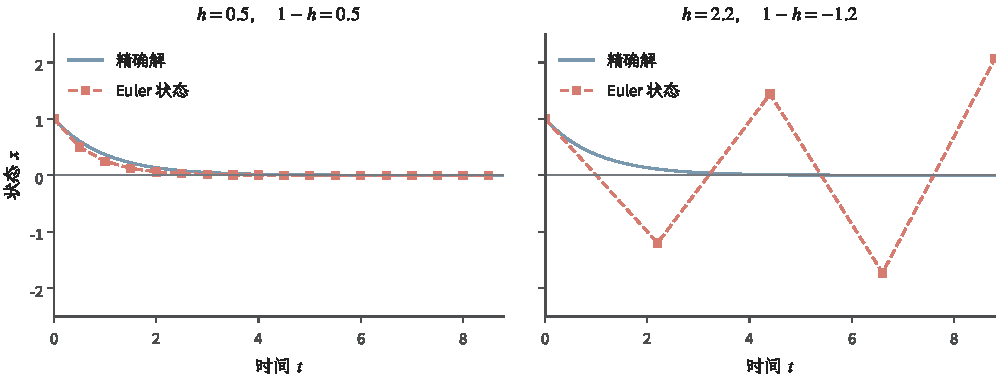
\includegraphics[width=\linewidth]{figures/01-mathematical-preliminaries/05-dynamical-systems-control-decision-and-games/matplotlib/dynamics/euler-stability.pdf}
  \caption{教学方程$\dot x=-x$、$x(0)=1$的精确解与Euler近似。蓝色实线为精确解，
  红色方点为数值状态；左图$h=0.5$衰减，右图$h=2.2$交替增长。两图采用相同坐标
  范围，连线只连接相邻数值状态。右图的发散来自步长，并非原连续系统不稳定。}
  \label{fig:dynamical-euler-stability}
\end{figure*}

\subsubsection{线性状态下的精确离散}

一般方法近似一步流，线性方程则可在规定的输入模型下直接积分。设
$[t_n,t_n+h)$内$\bm u(t)=\bm u_n$，对
式~\eqref{eq:dynamical-lti-variation-constants}取一个区间，得到
\begin{align}
  \bm x_{n+1}&=\bm A_h\bm x_n+\bm B_h\bm u_n,
    \label{eq:dynamical-zoh-discrete}\\
  \bm A_h&=\mathrm e^{h\bm A},\qquad
  \bm B_h=\int_0^h\mathrm e^{(h-s)\bm A}\bm B\,\mathrm ds.
    \label{eq:dynamical-zoh-matrices}
\end{align}
这称为\term{零阶保持}离散化。精确性针对区间内保持不变的输入，不表示真实输入
在区间内任意变化时也精确。若$\bm A$可逆，
$\bm B_h=\bm A^{-1}(\mathrm e^{h\bm A}-\bm I)\bm B$；$\bm A$奇异时继续使用积分
形式，不人为引入不存在的逆。输入保持误差与计算矩阵指数的数值误差仍可能存在，
只是没有Euler式的时间截断误差。

\subsubsection{保守状态下的几何离散}

对于可分Hamilton量，势能子系统保持位置、只改变动量；动能子系统保持动量、
只改变位置。两者各自可精确求解，因而可用对称分裂组成一步蛙跳：
\begin{align}
  \bm p_{n+1/2}&=\bm p_n-\frac h2\nabla U(\bm q_n),
    \label{eq:dynamical-leapfrog-half-momentum}\\
  \bm q_{n+1}&=\bm q_n+h\bm M^{-1}\bm p_{n+1/2},
    \label{eq:dynamical-leapfrog-position}\\
  \bm p_{n+1}&=\bm p_{n+1/2}-\frac h2\nabla U(\bm q_{n+1}).
    \label{eq:dynamical-leapfrog-final-momentum}
\end{align}
它是“动量半步、位置整步、动量半步”，不是把两条方程各做一次独立Euler更新。
令
$S_U^c(\bm q,\bm p)=(\bm q,\bm p-c\nabla U(\bm q))$、
$S_K^h(\bm q,\bm p)=(\bm q+h\bm M^{-1}\bm p,\bm p)$。
若$U\in C^2$，相应Jacobian为
\[
  \bm G_U=\begin{bmatrix}\bm I&\bm0\\-c\nabla^2U&\bm I\end{bmatrix},
  \qquad
  \bm G_K=\begin{bmatrix}\bm I&h\bm M^{-1}\\\bm0&\bm I\end{bmatrix}.
\]
三角结构使二者行列式均为$1$；$\nabla^2U$和$\bm M^{-1}$的对称性又给出
$\bm G_U^\top\bm J\bm G_U=\bm J$及
$\bm G_K^\top\bm J\bm G_K=\bm J$。故复合
$\Psi_h=S_U^{h/2}\circ S_K^h\circ S_U^{h/2}$保持体积且为辛映射。

每个子步换成负步长便是其逆，三步的对称排列使
$\Psi_h^{-1}=\Psi_{-h}$。若$R(\bm q,\bm p)=(\bm q,-\bm p)$是动量翻转，则还有
\[
  R\circ\Psi_h\circ R=\Psi_{-h}=\Psi_h^{-1}.
\]
因此这里的时间反演关系涉及动量翻转。把同一个映射连续应用两次便回到原态，
即$\Psi_h\circ\Psi_h=\operatorname{id}$，才称该映射为对合（involution）；
上面的逆映射关系不要求$\Psi_h$满足这个条件。
在足够光滑和固定有限时域下，蛙跳具有二阶全局精度。合适光滑性、轨迹有界及
小步长条件下的修正能量分析解释了常见的长时间有界能量振荡；辛性本身不保证
原Hamilton量每步完全相同。

\begin{example}[谐振子的精确与数值轨道]
  \label{ex:dynamical-harmonic-oscillator}
  取$U(q)=q^2/2,M=1$，精确解沿$q^2+p^2$的等值圆运动。蛙跳一步为
  \[
    \begin{bmatrix}q_{n+1}\\p_{n+1}\end{bmatrix}
    =
    \begin{bmatrix}1-h^2/2&h\\-h+h^3/4&1-h^2/2\end{bmatrix}
    \begin{bmatrix}q_n\\p_n\end{bmatrix}.
  \]
  更新矩阵的行列式为$1$、迹为$2-h^2$。当$0<h<2$时，其特征值是不同的
  单位模共轭数，并精确保持
  $(1-h^2/4)q_n^2+p_n^2$；这是一族椭圆，不是原来的能量圆。
  例如从$(1,0)$出发取$h=1$，一步得到$(1/2,-3/4)$，
  原能量从$1/2$变成$13/32$，却仍保持上述修正二次型。
  $h>2$时出现模大于$1$的特征值，$h=2$时还有退化导致的增长方向。
\end{example}
所以可逆、辛、体积保持与数值稳定分别需要检查。将这类轨迹用于随机采样时，
能量误差还需接受校正，不能把几何积分器直接当作精确采样器。

\subsection{仿射更新下的轨迹并行计算}

离散化选择数值规则，并行计算则重新安排同一规则的求值。对仿射递推
\begin{equation}
  \bm x_{t+1}=\bm A_t\bm x_t+\bm b_t,
  \label{eq:dynamical-affine-recurrence}
\end{equation}
用二元组$g_t=(\bm A_t,\bm b_t)$表示一步，定义较晚更新接在较早更新之后的复合为
\begin{equation}
  (\bm A_2,\bm b_2)\circ(\bm A_1,\bm b_1)
  =(\bm A_2\bm A_1,\bm A_2\bm b_1+\bm b_2).
  \label{eq:dynamical-affine-composition}
\end{equation}
复合结果仍是同维度仿射映射，这是能够紧凑表示整段更新的关键。三步直接核对得
\[
  \begin{aligned}
    g_3\circ(g_2\circ g_1)
    &=(\bm A_3\bm A_2\bm A_1,\,
       \bm A_3\bm A_2\bm b_1+\bm A_3\bm b_2+\bm b_3)\\
    &=(g_3\circ g_2)\circ g_1.
  \end{aligned}
\]
结合律允许用前缀扫描（prefix scan）同时求全部$g_{t-1}\circ\cdots\circ g_0$。
把更新按时间次序放在一棵平衡二叉树的叶子上，上行阶段合并相邻块，
每个内部节点保存自己整段的总复合。这个阶段只得到块的总映射，
全部中间状态还需要一次下传。

下传时，节点接收其区间之前已经完成的累计映射$p$。
左孩子继续接收$p$；若左块的总映射是$L$，右孩子就接收$L\circ p$。
根节点接收恒等映射$(\bm I,\bm0)$。例如四步$g_0,g_1,g_2,g_3$时，
左半块的总映射为$L=g_1\circ g_0$，四个叶子接收到的前缀分别是
\[
 \begin{aligned}
 p_0&=\operatorname{id},&p_1&=g_0,\\
 p_2&=L,&p_3&=g_2\circ L.
 \end{aligned}
\]
叶子$i$再形成$g_i\circ p_i$并作用于$\bm x_0$，便得到$\bm x_{i+1}$。
右块始终接在左块之后，所以这套下传规则也适用于不交换的复合。

总工作量统计所有节点执行的合并次数，计算深度统计最长依赖链上的合并次数。
$T$步形成的平衡树有$O(T)$个节点、$O(\log T)$层，
上下两阶段在每个节点只做常数次合并，同层互不依赖的节点可同时计算。
因此把一次固定维度合并视为一个操作时，总工作量为$O(T)$，深度为$O(\log T)$。
矩阵维度增长时，合并的实际算术成本仍需另算。

扫描保留时间次序。若$g_1(\bm x)=\operatorname{diag}(2,1)\bm x$、
$g_2(\bm x)=\bm x+(1,0)^\top$，则
\[
  (g_2\circ g_1)(\bm0)=(1,0)^\top,\qquad
  (g_1\circ g_2)(\bm0)=(2,0)^\top.
\]
这两个结果说明结合律不能换成交换律。浮点运算下，改变括号也可能改变舍入结果，
尤其是长乘积或条件数较大的传播；并行实现应按误差容限验证，而不是要求逐位相同。
若$\bm A_t,\bm b_t$只依赖事先给定的输入，仍可预先组成仿射扫描；若依赖尚未
算出的状态，或复合后不再有固定大小的封闭表示，就需要另行分析，不能直接套用。

\section{状态轨迹的极限与稳定}
\label{sec:dynamical-stability-sensitivity}

轨迹最终接近哪里，与小扰动会造成多大偏离，不是同一个问题。稳定方程可能在中途
放大误差，守恒轨迹也可能始终不接近任何一点。以下先统一这些性质的含义，再依据
线性或非线性结构选择判据。数值递推若另有步长误差，应把它作为另一个系统分析。

\subsection{状态轨迹的极限与稳定性质}

\begin{definition}[平衡点与稳定性]
  \label{def:dynamical-equilibrium-stability}
  考虑局部Lipschitz自治方程$\dot{\bm x}=\bm f(\bm x)$。
  满足$\bm f(\bm x^\star)=\bm0$的状态称为平衡点。以下性质均要求所涉及初值的
  解对全部$t\geq0$存在。

  平衡点在Lyapunov意义下\term{稳定}，是指对每个$\varepsilon>0$，存在
  $\delta>0$，使$\|\bm x(0)-\bm x^\star\|<\delta$蕴含
  $\|\bm x(t)-\bm x^\star\|<\varepsilon$对全部$t\geq0$成立。
  它具有局部吸引性，是指存在$r>0$，使所有
  $\|\bm x(0)-\bm x^\star\|<r$的解都趋于$\bm x^\star$。
  同时稳定且有局部吸引性称为\term{渐近稳定}。
  若存在$r,C,\alpha>0$，对上述$r$邻域内全部初值和$t\geq0$都有
  \[
    \|\bm x(t)-\bm x^\star\|_2
    \leq C\mathrm e^{-\alpha t}\|\bm x(0)-\bm x^\star\|_2,
  \]
  则称为局部指数稳定。若同一估计对全部初值成立，则称为全局指数稳定。
\end{definition}
离散时间把$t\geq0$换成非负整数，平衡条件换成
$F(\bm x^\star)=\bm x^\star$，指数因子可写成$q^t$，其中$0<q<1$。
“最终接近”与“始终不远离”分别对应吸引与稳定；不能只展示一条收敛轨迹，
便省去邻域内全部初值的量词。指数条件还要求$C,\alpha$在整个邻域统一。

\begin{table*}[htbp]
  \centering
  \begin{tabularx}{\linewidth}{lXXX}
    \toprule
    方程与原点 & 小初值始终小 & 轨迹趋于原点 & 统一指数衰减\\
    \midrule
    $\dot x=0$ & 是，状态保持初值 & 否，非零初值不动 & 否\\
    $\dot x=-x^3$ & 是，$|x(t)|$不增 & 是，代数衰减 & 否\\
    $\dot x=-x$ & 是 & 是 & 是，$|x(t)|=\mathrm e^{-t}|x(0)|$\\
    \bottomrule
  \end{tabularx}
  \caption{零输入下原点的稳定性质。第二行的解为
  $x(t)=x(0)/\sqrt{1+2x(0)^2t}$，它回到原点但不具有统一指数速度。
  三种方程均有全局解，比较不涉及数值离散。}
  \label{tab:dynamical-stability-types}
\end{table*}

有些轨迹不趋于一点，而是长期绕着一个集合运动。对此需要集合版本的描述。
\begin{definition}[不变集合与轨迹极限集]
  \label{def:dynamical-invariant-limit-sets}
  设$\Phi_t$是局部Lipschitz自治方程的流，并要求所述集合上的解正向全局存在。
  若$\Phi_t(\Omega)\subseteq\Omega$对全部$t\geq0$成立，则$\Omega$为
  \term{正向不变集}。若$\Phi_t(M)=M$对全部$t\geq0$成立，则$M$为
  \term{不变集}；这还要求集合内每一点有任意长时间以前的集合内前像，等价于
  每点都位于始终留在集合内的完整轨迹上。
  对正向有界轨迹，定义其\term{$\omega$极限集}为
  \[
    \omega(\bm x_0)=
    \{\bm z:\text{存在 }t_j\to\infty\text{ 使 }\bm x(t_j)\to\bm z\}.
  \]
\end{definition}
正向不变集限制一批初值的全部未来，极限集则记录一条轨迹在越来越晚的时刻反复
靠近的状态。趋于集合指到该集合的距离趋零，不要求在集合内部停止运动。

为了不逐条求解轨迹，常寻找一个能度量离开平衡点程度的标量。以原点为平衡，
$V\in C^1(D)$若满足$V(\bm0)=0$且非零点上$V>0$，称为正定的Lyapunov候选。
“候选”只说明它有合适的空间形状，还没有证明沿轨迹的变化方向。
\begin{definition}[Lyapunov函数]
  \label{def:dynamical-lyapunov-function}
  对$\dot{\bm x}=\bm f(\bm x)$，若上述正定候选还满足
  $\dot V(\bm x):=\nabla V(\bm x)^\top\bm f(\bm x)\leq0$，
  则称其为该邻域内的\term{Lyapunov函数}；若非零点处严格小于零，
  则称为严格Lyapunov函数。
\end{definition}
它不必等于物理能量。离散方程相应检查
$V(F(\bm x))-V(\bm x)$。正定性使“小能量”确实限制所有状态方向，
非增性才保证轨迹不能穿越更高的能量边界。下面的线性与非线性判据共同使用这两项。

\subsection{线性演化下的轨迹稳定性}

\subsubsection{长期演化的谱判据}

离散齐次系统为
\begin{equation}
  \bm x_{t+1}=\bm A\bm x_t,\qquad \bm x_t=\bm A^t\bm x_0.
  \label{eq:dynamical-discrete-linear-homogeneous}
\end{equation}
矩阵的幂、Jordan分解与指数已在第~\ref{chap:matrix-analysis}章建立。这里用它们
把长期轨迹问题化成谱的位置。
\begin{theorem}[离散线性系统的渐近稳定性]
  \label{thm:dynamical-discrete-spectral-stability}
  式~\eqref{eq:dynamical-discrete-linear-homogeneous}的原点全局渐近稳定，
  当且仅当$\rho(\bm A)=\max_{\lambda\in\operatorname{spec}(\bm A)}|\lambda|<1$。
  在此条件下，原点实际上全局指数稳定。
\end{theorem}
\begin{proof}
  在复数域写$\bm A=\bm V\bm J\bm V^{-1}$。大小为$r$的Jordan块
  $\bm J_\lambda=\lambda\bm I+\bm N$满足
  \[
    \bm J_\lambda^t
      =\sum_{j=0}^{\min(t,r-1)}\binom tj\lambda^{t-j}\bm N^j.
  \]
  $\lambda=0$的块在有限步后为零；$0<|\lambda|<1$时，多项式因子被几何衰减
  压过。取$\rho(\bm A)<q<1$，全部有限个块可统一控制为$Cq^t$，乘回换基矩阵
  得$\|\bm A^t\|\leq C' q^t$。它既给出趋零，也给出稳定性所需的统一有界增益。
  反之，若存在$|\lambda|\geq1$，沿其特征向量的复轨迹不趋零；分解成实部与虚部，
  至少一条实轨迹不趋零。单位模特征值的非平凡Jordan块还可能多项式增长。
  故渐近稳定要求全部特征值严格在单位圆内。
\end{proof}

\begin{theorem}[连续线性系统的指数稳定性]
  \label{thm:dynamical-continuous-spectral-stability}
  系统$\dot{\bm x}=\bm A\bm x$的原点全局指数稳定，当且仅当$\bm A$的全部
  特征值实部严格为负。这样的矩阵称为Hurwitz矩阵。
\end{theorem}
\begin{proof}
  对Jordan块，
  $\mathrm e^{t(\lambda\bm I+\bm N)}
   =\mathrm e^{\lambda t}\sum_{j=0}^{r-1}t^j\bm N^j/j!$。
  若全部实部为负，取$0<\alpha<-\max_\lambda\operatorname{Re}\lambda$，
  有限次多项式乘指数可统一控制为$C\mathrm e^{-\alpha t}$。乘回换基矩阵就得到
  $\|\mathrm e^{t\bm A}\|\leq C'\mathrm e^{-\alpha t}$。
  若某个特征值实部非负，则对应实不变子空间中存在增长、常值或不衰减振荡的轨迹，
  不可能满足该指数界。非平凡Jordan块不会消除这种障碍。
\end{proof}
连续系统检查左半平面，离散系统检查单位圆。边界上的谱需另查Jordan结构：
可能稳定而不吸引，也可能增长，不能把严格不等号改成非严格不等号。

谱给出长期方向，二次能量给出一个可逐时刻检查的证书。取
$V(\bm x)=\bm x^\top\bm P\bm x$，其中$\bm P\succ\bm0$，则
\begin{equation}
  \dot V=\bm x^\top(\bm A^\top\bm P+\bm P\bm A)\bm x.
  \label{eq:dynamical-continuous-lyapunov-derivative}
\end{equation}
\begin{theorem}[线性Lyapunov方程]
  \label{thm:dynamical-linear-lyapunov-equation}
  $\bm A$为Hurwitz矩阵，当且仅当对每个$\bm Q\succ\bm0$，存在唯一
  $\bm P\succ\bm0$满足
  \begin{equation}
    \bm A^\top\bm P+\bm P\bm A=-\bm Q.
    \label{eq:dynamical-continuous-lyapunov-equation}
  \end{equation}
\end{theorem}
\begin{proof}
  若$\bm A$为Hurwitz矩阵，定义
  $\bm P=\int_0^\infty\mathrm e^{t\bm A^\top}\bm Q\mathrm e^{t\bm A}\,\mathrm dt$。
  指数稳定保证积分收敛。任意非零$\bm x$对应的被积二次型非负，且在$t=0$
  严格为正，所以$\bm P\succ\bm0$。对被积矩阵求导并积分，得
  \[
    \bm A^\top\bm P+\bm P\bm A
    =[\mathrm e^{t\bm A^\top}\bm Q\mathrm e^{t\bm A}]_0^\infty=-\bm Q.
  \]
  两解之差$\bm D$满足$\bm A^\top\bm D+\bm D\bm A=\bm0$，故
  $\mathrm e^{t\bm A^\top}\bm D\mathrm e^{t\bm A}$恒为$\bm D$；
  令$t\to\infty$得$\bm D=\bm0$。

  反之，若存在正定的$\bm P,\bm Q$满足方程，记
  $p_-=\lambda_{\min}(\bm P)$、$p_+=\lambda_{\max}(\bm P)$、
  $q_-=\lambda_{\min}(\bm Q)$。则
  $p_-\|\bm x\|_2^2\leq V\leq p_+\|\bm x\|_2^2$，且
  $\dot V=-\bm x^\top\bm Q\bm x\leq-(q_-/p_+)V$。
  乘以积分因子得到
  \[
    \|\bm x(t)\|_2
    \leq\sqrt{p_+/p_-}\,
      \mathrm e^{-q_-t/(2p_+)}\|\bm x(0)\|_2.
  \]
  这直接证明指数稳定；由已证谱判据，$\bm A$为Hurwitz矩阵。
\end{proof}
反向证明只用二次型上下界与积分估计，不依赖尚未建立的非线性判据。

\begin{theorem}[离散时间Lyapunov方程]
  \label{thm:dynamical-discrete-lyapunov-equation}
  $\rho(\bm A)<1$，当且仅当对每个$\bm Q\succ\bm0$，存在唯一
  $\bm P\succ\bm0$满足$\bm A^\top\bm P\bm A-\bm P=-\bm Q$。
\end{theorem}
\begin{proof}
  正向取
  $\bm P=\sum_{j=0}^\infty(\bm A^\top)^j\bm Q\bm A^j$。
  上述离散指数界使级数绝对收敛；首项正定、其余项半正定，故$\bm P$正定。
  左乘$\bm A^\top$、右乘$\bm A$后相减即得方程。两解之差满足
  $\bm D=(\bm A^\top)^t\bm D\bm A^t$，令$t\to\infty$得唯一性。
  反向用$V(\bm x)=\bm x^\top\bm P\bm x$，有
  \[
    V(\bm A\bm x)-V(\bm x)=-\bm x^\top\bm Q\bm x<0
    \quad(\bm x\neq\bm0).
  \]
  比值$V(\bm A\bm x)/V(\bm x)$在单位球面上连续且严格小于$1$，
  因紧性有统一上界$c<1$，且$c\geq0$。于是$V(\bm x_t)\leq c^t V(\bm x_0)$
  （$c=0$时一步后即为零）。二次型界给出指数稳定，再由谱判据得到$\rho(\bm A)<1$。
\end{proof}
线性系统因此总能为稳定动力学找到某个二次能量，但这个能量一般不是欧氏范数平方。
下一项正说明更换度量为什么重要。

\subsubsection{有限时间的瞬态放大}

取
\[
  \bm A=\begin{bmatrix}1/2&K\\0&1/2\end{bmatrix},\qquad K>0.
\]
无论$K$多大，谱半径均为$1/2$，而
\[
  \bm A^t=
  \begin{bmatrix}
    2^{-t}&tK\,2^{-(t-1)}\\0&2^{-t}
  \end{bmatrix}.
\]
从$\bm x_0=(0,1)^\top$出发，第一步即为$(K,1/2)^\top$，欧氏范数可以大幅
增长；之后$t2^{-t}\to0$才使状态趋零。这里放大来自第二坐标向第一坐标的耦合，
没有任何输入或数值误差。

\begin{figure}[htbp]
  \centering
  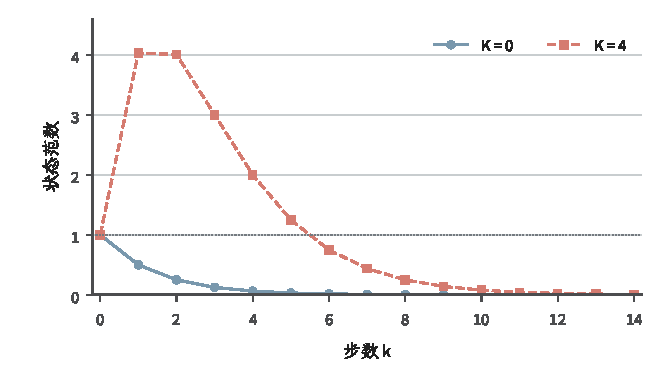
\includegraphics[width=\linewidth]{figures/01-mathematical-preliminaries/05-dynamical-systems-control-decision-and-games/matplotlib/concepts-dynamics/transient-growth.pdf}
  \caption{同谱系统的不同瞬态。初值均为$(0,1)^\top$，蓝色圆点取$K=0$，
  红色方点取$K=4$，谱半径均为$1/2$。后者前两步范数约为$4.03$、$4.01$，
  随后才趋零；灰线为初始范数$1$。长期衰减不等于每一步都收缩。}
  \label{fig:dynamical-transient-growth}
\end{figure}

$K\neq0$时，$\bm A^\top\bm A\neq\bm A\bm A^\top$，矩阵非正规。
本例只有一个独立特征向量，幂零耦合产生$t2^{-t}$项；可对角化但特征向量近乎
共线的非正规矩阵，也可能因模态先相消、后分离而放大。有限时间增益
$\|\bm A^t\|$、伪谱与合适的Lyapunov范数描述了谱半径以外的信息。
谱稳定没有许诺欧氏范数下逐步收缩，更没有许诺中间状态不越过任务边界。

\subsection{非线性演化下的轨迹稳定性}

\subsubsection{平衡邻域内的稳定判据}

非线性系统一般无法通过一个固定矩阵构造全局二次能量，因而需要寻找候选函数。
它可以来自物理能量、误差平方或模型特有的守恒与耗散关系。找到候选以后，
仍须检查正定性、沿轨迹导数以及适用区域。\scite{math-khalil2002nonlinear}
\begin{theorem}[连续时间Lyapunov判据]
  \label{thm:dynamical-nonlinear-lyapunov}
  设原点为$\dot{\bm x}=\bm f(\bm x)$的平衡点，$\bm f$在其邻域内局部Lipschitz。
  若该邻域存在$C^1$正定候选$V$且$\dot V\leq0$，则原点稳定；
  若非零点上$\dot V<0$，则原点局部渐近稳定。
  若这些条件在$\mathbb R^d$上成立，且$V(\bm x)\to\infty$当
  $\|\bm x\|\to\infty$，则所有解正向全局存在；非增情形给出稳定性，
  严格下降情形给出全局渐近稳定性。
\end{theorem}
\begin{proof}
  选足够小的$\varepsilon$使闭球位于适用邻域。球面上的连续正函数$V$有
  最小值$c_\varepsilon>0$。原点处连续性给出$\delta<\varepsilon$，
  使$\|\bm x_0\|<\delta$时$V(\bm x_0)<c_\varepsilon$。
  轨迹若首次触及球面，必须达到至少$c_\varepsilon$的能量，与$\dot V\leq0$
  矛盾。更具体地，可选$\bm x_0$所在的闭子水平集与闭球的交作为紧集$K$，
  且其能量水平严格低于球面最小值；轨迹不能穿出$K$，局部解可延拓到任意正时间。
  对全部足够小$\varepsilon$得到此结论即为稳定性。

  若$\dot V$在非零点严格为负，反设某条上述轨迹不趋零，则存在$\varepsilon_0>0$
  及$t_j\to\infty$，使$\|\bm x(t_j)\|\geq\varepsilon_0$。
  在紧集$K$上令$M=\sup_K\|\bm f\|$。非零轨迹下可取$M>0$；
  速度有界使每次达到该半径后至少在长度$\varepsilon_0/(2M)$内保持
  $\|\bm x\|\geq\varepsilon_0/2$。函数$-\dot V$在
  $K\cap\{\|\bm x\|\geq\varepsilon_0/2\}$上有严格正下界。
  选取互不相交的这些时间段，能量便减少无穷大量，与$V\geq0$矛盾。
  因而轨迹趋零。全局且径向无界时，每个初值的子水平集都紧；
  同样的延拓与下降论证适用于任意初值，得到全局结论。
\end{proof}
径向无界性控制的是远处状态，不能用“在原点附近正定”代替。
若还能找到$c_1,c_2,c_3>0$使
$c_1\|\bm x\|^2\leq V\leq c_2\|\bm x\|^2$、$\dot V\leq-c_3\|\bm x\|^2$，
则前述线性方程证明中的积分估计同样给出局部指数衰减。一般严格负导数未必有
这种二次型比较，所以渐近稳定未必指数稳定。

\subsubsection{不变区域内的极限集合}

机械能常只在某些方向上直接耗散，导致$\dot V=0$的集合远大于平衡点。
这时应问：轨迹能否一直留在这个集合中？LaSalle原理把这个问题转成极限集合判据。
\begin{theorem}[LaSalle不变性原理]
  \label{thm:dynamical-lasalle-invariance}
  设自治向量场$\bm f$局部Lipschitz，$\Omega$紧且正向不变，
  $V$在包含$\Omega$的开邻域上为$C^1$，并有$\dot V\leq0$。
  令$E=\{\bm x\in\Omega:\dot V(\bm x)=0\}$，$M$为$E$中最大不变集，
  则从$\Omega$出发的每条轨迹满足
  $\operatorname{dist}(\bm x(t),M)\to0$。
\end{theorem}
\begin{proof}
  紧性排除有限时间逃逸，也使$\omega(\bm x_0)$非空且紧。
  沿轨迹的$V$单调不增且有下界，故趋于$v_\infty$。
  对极限点$\bm z=\lim_j\bm x(t_j)$，连续性给出$V(\bm z)=v_\infty$。

  对固定$s\geq0$，流的初值连续性使
  $\bm x(t_j+s)\to\Phi_s(\bm z)$，故
  $\Phi_s(\omega(\bm x_0))\subseteq\omega(\bm x_0)$。
  反过来，充分大的$j$有$t_j>s$。紧性允许从$\bm x(t_j-s)$取收敛子列，
  其极限$\bm w$属于$\omega(\bm x_0)$，且$\Phi_s(\bm w)=\bm z$。
  因此$\Phi_s(\omega(\bm x_0))=\omega(\bm x_0)$，这里得到的是完整不变性，
  而非仅正向不变性。

  $V$在极限集上恒为$v_\infty$，从其中任一点出发的轨迹仍在该集合，
  所以沿轨迹导数为零。于是$\omega(\bm x_0)$是$E$内的不变集，必包含于$M$。
  若到$M$的距离不趋零，就有$\varepsilon>0$及$t_j\to\infty$使距离至少为
  $\varepsilon$。紧性再给出收敛子列，其极限属于$\omega(\bm x_0)\subseteq M$，
  与此距离下界矛盾。
\end{proof}

\begin{example}[阻尼振子的零导数集合]
  \label{ex:dynamical-damped-oscillator-lasalle}
  对$\dot q=p,\dot p=-q-cp$，其中$c>0$，取$V=(q^2+p^2)/2$，则
  $\dot V=q p+p(-q-cp)=-cp^2\leq0$。
  零导数集合为$p=0$；但其上$q\neq0$的点满足$\dot p=-q\neq0$，
  马上离开该直线。因此零导数集合中最大不变集只有原点。
  每个能量子水平集均紧且正向不变，LaSalle原理遂给出所有轨迹趋于原点。
\end{example}

\begin{figure}[htbp]
  \centering
  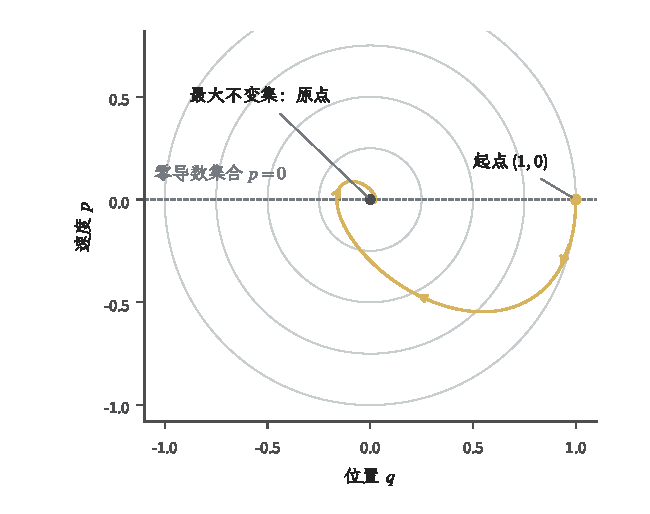
\includegraphics[width=\linewidth]{figures/01-mathematical-preliminaries/05-dynamical-systems-control-decision-and-games/matplotlib/teaching-dynamics/lasalle-zero-set.pdf}
  \caption{阻尼振子$\dot q=p,\dot p=-q-p$从$(1,0)$出发的精确轨迹。
  黄色轨迹覆盖$t=0$至$12$，箭头指示时间；灰色虚线为$\dot V=0$的直线$p=0$，
  浅灰圆为能量参考等值线。起点虽在零导数集合上，初始速度$(0,-1)$却将它带离
  该集合；能一直留在其中的完整轨迹只有原点。}
  \label{fig:reader-lasalle-zero-set}
\end{figure}
能量非增先限制活动区域，动力学再排除不能持续停留的零导数点。
把整个$E$直接称为“最终状态”，会丢掉LaSalle论证中最关键的一步。

\subsection{初值与输入扰动下的轨迹稳定性}

前述原点判据通常对应零输入，或把恒定输入下的平衡平移到原点。
温度例的恒定$u_t=0.4$对应平衡$2$，误差$e_t=x_t-2$才满足$e_{t+1}=0.8e_t$。
不能因为误差趋零，就说实际温度趋于环境温度。

对连续方程，若$\bm f$关于状态具有Lipschitz常数$L$，同一输入下两条解满足
\[
  \|\bm x(t)-\widetilde{\bm x}(t)\|
  \leq \mathrm e^{L(t-t_0)}\|\bm x_0-\widetilde{\bm x}_0\|.
\]
这是由积分方程与引理~\ref{lem:action-state-gronwall}得到的有限时间连续依赖，
在$L>0$时没有声称衰减。若输入也不同、$\bm f$关于输入的Lipschitz常数为$L_u$，
并且比较模型沿第二条轨迹还有大小至多$r(s)$的向量场误差，则同一引理给出
\[
  \|\bm x(t)-\widetilde{\bm x}(t)\|
  \leq \mathrm e^{L(t-t_0)}\|\bm x_0-\widetilde{\bm x}_0\|
  +\int_{t_0}^t\mathrm e^{L(t-s)}
     \bigl(L_u\|\bm u(s)-\widetilde{\bm u}(s)\|+r(s)\bigr)\,\mathrm ds.
\]
初态误差、输入误差、模型误差因此有不同来源，却都要经过后续动态传播。

对指数稳定线性系统，若
$\|\mathrm e^{t\bm A}\|\leq M\mathrm e^{-\alpha t}$，常数变易公式给出更强的界：
\[
  \|\bm x(t)\|
  \leq M\mathrm e^{-\alpha(t-t_0)}\|\bm x_0\|
  +M\|\bm B\|\int_{t_0}^t\mathrm e^{-\alpha(t-s)}\|\bm u(s)\|\,\mathrm ds.
\]
若$\|\bm u(s)\|\leq U$，第二项至多
$(M\|\bm B\|U/\alpha)(1-\mathrm e^{-\alpha(t-t_0)})$。
有界输入产生有界状态，但持续输入通常留下非零稳态。
离散温度例若输入固定偏多$\delta u$，稳态偏差就是
$\delta u/(1-0.8)=5\delta u$。稳定性消退初值记忆，不会自动消除持续施加的偏差。

\section{随机状态与随机轨迹}
\label{sec:dynamical-ito-fokker-planck}

给定相同初温与加热量，开门、风速等未显式建模的作用仍可能改变真实温度。
把这些作用表示成过程噪声后，更新公式不再只产生一条确定轨迹，而是把噪声的联合
规律转换为状态的联合规律。本节只研究这种生成机制，尚未用任何传感器读数条件化。
离散更新可以直接逐步随机生成；连续时间必须先说明随机增量怎样累计。

\subsection{随机状态的离散演化}

\subsubsection{随机递推与状态转移}

在同一概率空间上给定初始状态、输入及背景随机量，写
\[
  \bm x_{t+1}=F_t(\bm x_t,\bm u_t,\bm\varepsilon_{t+1}).
\]
若$\bm\varepsilon_{t+1}$独立于已有状态历史，分布为$\nu_{t+1}$，且$F_t$可测，
并将本节的输入$(\bm u_t)$固定为预先给定的确定序列，则由更新映射得到转移核
\[
  K_t(\bm x,A)=\int
    \mathbb I\{F_t(\bm x,\bm u_t,\bm e)\in A\}\,\nu_{t+1}(\mathrm d\bm e).
\]
对每个$\bm x$它是概率分布，对每个可测$A$它关于$\bm x$可测，符合
定义~\ref{def:probability-kernel}。独立性使
$\mathbb P(\bm x_{t+1}\in A\mid\bm x_{0:t})=K_t(\bm x_t,A)$，
这才得到当前状态的Markov性质。给定$\pi_0=\mathcal L(\bm x_0)$，整条有限轨迹满足
\[
  \mathbb P(\bm x_{0:T}\in\mathrm d\bm z_{0:T})
  =\pi_0(\mathrm d\bm z_0)
    \prod_{t=0}^{T-1}K_t(\bm z_t,\mathrm d\bm z_{t+1}),
\]
其中乘积表示逐次核积分。它同时规定跨时刻依赖，而不只是各个时刻的边缘分布。
若以后改用仅依赖当前状态的可测反馈$\bm u_t=\pi_t(\bm x_t)$，
把$\pi_t(\bm x)$代入核即可。若输入还依赖更早的状态或带噪观测，
仅有新噪声独立通常不足以使$\bm x_t$本身为Markov状态；
须保留相应历史或扩充状态。这一区别将在
第~\ref{chap:control-theory}章“策略的实现与轨迹控制”中用于规定可实施策略。

常用的线性加性模型为
\begin{equation}
  \bm x_{t+1}=\bm A_t\bm x_t+\bm B_t\bm u_t+\bm w_{t+1}.
  \label{eq:dynamical-linear-state-model}
\end{equation}
若$\bm w_{t+1}\sim\mathcal N(\bm0,\bm Q_{t+1})$且独立于初态与其他过程噪声，
$K_t(\bm x,\cdot)=\mathcal N(\bm A_t\bm x+\bm B_t\bm u_t,\bm Q_{t+1})$。
即便$\bm Q_{t+1}$奇异，它仍是合法概率核，只是不一定有全维Lebesgue密度。

相关噪声需要重新检查条件结构。例如
$x_{t+1}=a x_t+w_{t+1}$，而$w_{t+1}=\rho w_t+\varepsilon_{t+1}$，
其中新$\varepsilon$独立。代入$w_t=x_t-a x_{t-1}$得
$x_{t+1}=(a+\rho)x_t-\rho a x_{t-1}+\varepsilon_{t+1}$。
一般仅给$x_t$已不足够；可把$(x_t,w_t)$扩成状态，或保留对更长历史的条件依赖。
“递推里有噪声”不等于“当前状态是Markov的”。

温度模型现在恢复为
\[
  x_{t+1}=0.8x_t+u_t+w_{t+1},\qquad
  w_{t+1}\sim\mathcal N(0,0.04).
\]
取各$w_t$相互独立且独立于初态。若$x_0=0,u_t=0.4$，
则$\mathbb E x_t=2(1-0.8^t)$，过程方差为
$0.04\sum_{j=0}^{t-1}0.8^{2j}$。平均轨迹仍与无噪模型相同，一条实际轨迹却会
在其附近波动。图~\ref{fig:action-state-temperature-layers}再叠加
$y_t=x_t+v_t$、$v_t\sim\mathcal N(0,0.09)$的独立读数噪声，
先展示生成层次；怎样由读数推断状态留到观测部分。

\begin{figure*}[htbp]
  \centering
  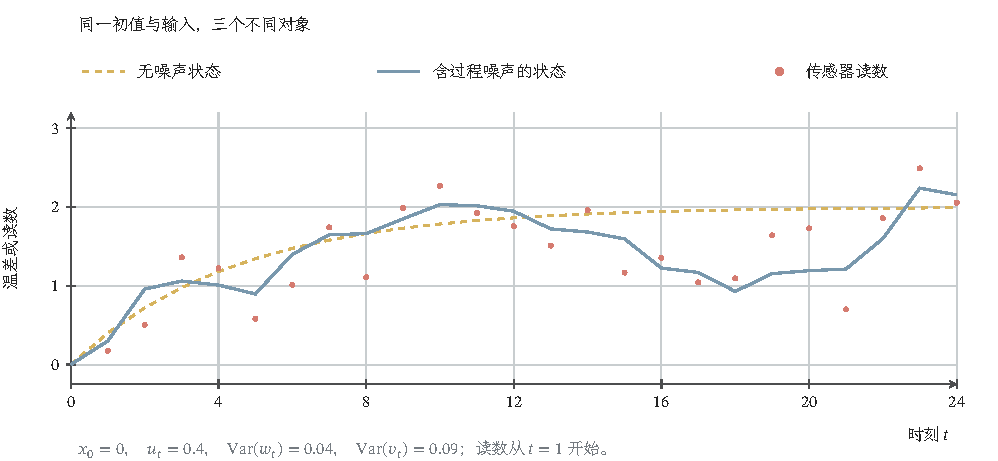
\includegraphics[width=\linewidth]{figures/01-mathematical-preliminaries/05-dynamical-systems-control-decision-and-games/tikz/dynamics/temperature-state-observation.pdf}
  \caption{同一温度模型的三个对象。初态$x_0=0$，输入始终为$0.4$；
  无噪声轨迹趋于$2$，过程噪声改变真实状态，独立观测噪声又把真实状态变成带噪读数。
  噪声方差分别为$0.04$和$0.09$。图中带噪曲线是固定种子的教学模拟，
  不是置信区间，也没有把读数用于反向校正状态。}
  \label{fig:action-state-temperature-layers}
\end{figure*}

\subsubsection{单时间尺度的随机逼近}
\label{sec:stoch-approximation-markov-noise}

有些递推状态不是房间温度，而是希望逐步求出的参数。设未知均值为$\mu$，
目标是解平均方程
\begin{equation}
  h(\theta)=\mathbb E[Y-\theta]=\mu-\theta=0.
  \label{eq:stoch-mean-root}
\end{equation}
每次只能得到一个含噪观测，仍可沿观测建议的方向作小步移动。这就是
\term{随机逼近}：用随机逐步更新寻找平均漂移的根，或其稳定不变对象。
算法轮次以括号上标标记，区别于物理状态的时间下标。
一般形式为
\begin{equation}
  \bm\theta^{(t+1)}=\bm\theta^{(t)}+\alpha_t
   [\overline{\bm h}(\bm\theta^{(t)})+\bm\xi_{t+1}+\bm r_{t+1}],
  \label{eq:stoch-general-stochastic-approximation}
\end{equation}
其中$\alpha_t>0$是步长，$\overline{\bm h}$是平均漂移，
$\mathbb E[\bm\xi_{t+1}\mid\mathcal F_t]=\bm0$是鞅差噪声，
$\bm r_{t+1}$记录近似、截断或尚未平衡所致的偏差。
Markov观测一般不能直接作为这个鞅差，稍后将分解其累计误差。

均值问题的Robbins--Monro递推为
\begin{equation}
  \theta^{(t+1)}=\theta^{(t)}
       +\alpha_t(Y_{t+1}-\theta^{(t)}).
  \label{eq:stoch-robbins-monro-mean}
\end{equation}
观测高于当前估计就上移，低于估计就下移。若
$\mathbb E[Y_{t+1}\mid\mathcal F_t]=\mu$，条件平均方向恰为$\mu-\theta^{(t)}$。
取$\alpha_t=1/(t+1)$时，第一步完全采用$Y_1$；归纳得
$\theta^{(t)}=t^{-1}\sum_{s=1}^tY_s$。一般步长对应不等权的递推，
所以随机逼近不限于样本平均。\scite{math-robbins1951stochastic}

经典递减步长条件是
\begin{equation}
  \sum_{t=0}^\infty\alpha_t=\infty,\qquad
  \sum_{t=0}^\infty\alpha_t^2<\infty.
  \label{eq:stoch-robbins-monro-stepsizes}
\end{equation}
前者保留无限的累计移动能力；若鞅差噪声的条件二阶矩有统一上界，
后者就能控制累计的加权方差。具体地，对此前信息$\mathcal F_t$和鞅差$\xi_{t+1}$，
若$\mathbb E[\xi_{t+1}^2\mid\mathcal F_t]\leq\sigma^2$，则
\[
 \sum_{t=0}^\infty\alpha_t^2
 \mathbb E[\xi_{t+1}^2\mid\mathcal F_t]
 \leq\sigma^2\sum_{t=0}^\infty\alpha_t^2<\infty.
\]
仅有每个时刻的方差有限还不够，因为这些方差可能随时间无界增长。
$\alpha_t=c/(t+t_0)^\gamma$在$c,t_0>0$、$1/2<\gamma\leq1$时满足两项。
若步长和有限，初始误差可能尚未消除就停止有效移动；若平方和无穷，
上述噪声控制不再适用，但这本身也不是任意模型必然发散的断言。

固定步长则保留持续响应新数据的能力。对独立同分布、均值$\mu$、方差$\sigma^2$
的观测，确定初值及$\alpha_t=\alpha\in(0,1)$给出
\[
  e_{t+1}=(1-\alpha)e_t+\alpha(Y_{t+1}-\mu),\qquad
  \mathbb E e_t=(1-\alpha)^t e_0.
\]
由独立性，方差$v_{t+1}=(1-\alpha)^2v_t+\alpha^2\sigma^2$，因而
\[
  v_t=\frac{\alpha\sigma^2}{2-\alpha}
       [1-(1-\alpha)^{2t}]
  \longrightarrow\frac{\alpha\sigma^2}{2-\alpha}.
\]
初始偏差消失，随机波动却留下正的稳态方差。小步长降低此误差，也延缓对初值或
目标变化的响应。这是固定均值模型的精确计算，不能替代一般非线性递推的稳定证明。

\begin{figure*}[htbp]
  \centering
  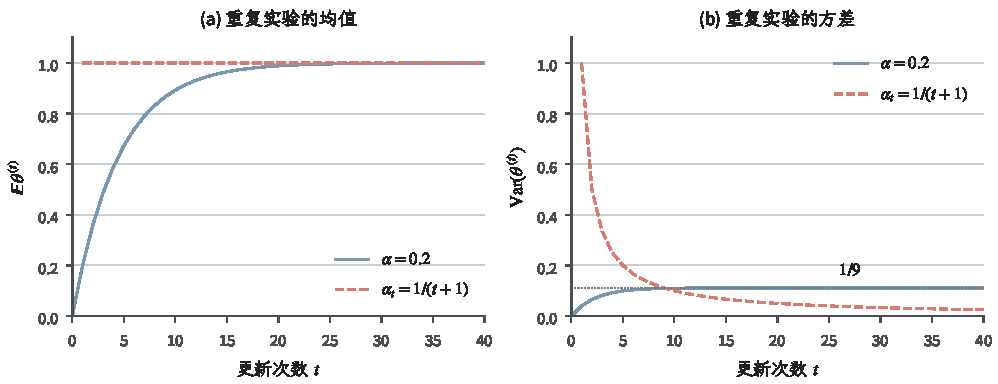
\includegraphics[width=\linewidth]{figures/01-mathematical-preliminaries/05-dynamical-systems-control-decision-and-games/matplotlib/concepts-probability/stochastic-stepsize-bias-variance.pdf}
  \caption{同一均值问题的重复实验均值与方差。取$\theta^{(0)}=0,\mu=1,\sigma^2=1$，
  观测独立同分布；蓝实线为固定$\alpha=0.2$，红虚线为$\alpha_t=1/(t+1)$。
  固定步长方差趋于$1/9$，样本平均方差为$1/t$。曲线由解析式得到，不是一条样本轨迹。}
  \label{fig:stochastic-stepsize-bias-variance}
\end{figure*}

要把“噪声越来越小”变成逐路径收敛，需要控制累计噪声，而不只计算单步均值。
下面保留一个可完整证明的代表性结论。
\begin{lemma}[带可求和误差的非负超鞅]
  \label{lem:stoch-almost-supermartingale}
  设$Z_t,A_t$为关于$\mathcal F_t$的非负可积适应过程，$b_t\geq0$为确定数，
  且$\mathbb E[Z_{t+1}\mid\mathcal F_t]\leq Z_t-A_t+b_t$。
  若$\sum_tb_t<\infty$，则$Z_t$几乎必然收敛到有限随机变量，
  且$\sum_tA_t<\infty$几乎必然成立。
\end{lemma}
\begin{proof}
  令$r_t=\sum_{s=t}^\infty b_s$、$U_t=Z_t+r_t$。因为$r_t=b_t+r_{t+1}$，
  有$\mathbb E[U_{t+1}\mid\mathcal F_t]\leq U_t-A_t$。
  $U_t$是非负超鞅，由非负超鞅收敛定理几乎必然收敛到有限值。
  取期望并累加得到
  $\mathbb E\sum_{t=0}^nA_t\leq\mathbb E U_0$。
  单调收敛给出$\mathbb E\sum_{t=0}^\infty A_t\leq\mathbb E U_0<\infty$，
  所以该非负级数几乎必然有限。又$r_t\to0$，故$Z_t=U_t-r_t$也收敛。
\end{proof}
其中的鞅与超鞅收敛工具见第~\ref{chap:stochastic-processes-and-approximation}章；
本引理把可求和误差吸收到一个真正的超鞅中。

\begin{theorem}[均值求根的几乎必然收敛]
  \label{thm:stoch-mean-root-convergence}
  设$\mathcal F_t$包含$\theta^{(0)},Y_1,\ldots,Y_t$，且
  $\mathbb E[(\theta^{(0)}-\mu)^2]<\infty$。若
  \[
    \mathbb E[Y_{t+1}\mid\mathcal F_t]=\mu,\qquad
    \mathbb E[(Y_{t+1}-\mu)^2\mid\mathcal F_t]\leq\sigma^2,
  \]
  步长满足式~\eqref{eq:stoch-robbins-monro-stepsizes}并最终有$0<\alpha_t\leq1$，
  则式~\eqref{eq:stoch-robbins-monro-mean}的$\theta^{(t)}\to\mu$几乎必然成立。
\end{theorem}
\begin{proof}
  记$e_t=\theta^{(t)}-\mu$、$\xi_{t+1}=Y_{t+1}-\mu$，则
  $e_{t+1}=(1-\alpha_t)e_t+\alpha_t\xi_{t+1}$。
  初值与条件二阶矩假设递归保证每个有限时刻的$\mathbb E e_t^2$有限。
  舍去有限前缀，令$0<\alpha_t\leq1$。条件展开平方，交叉项为零，得到
  \[
    \mathbb E[e_{t+1}^2\mid\mathcal F_t]
    =(1-\alpha_t)^2e_t^2
      +\alpha_t^2\mathbb E[\xi_{t+1}^2\mid\mathcal F_t]
    \leq e_t^2-\alpha_te_t^2+\alpha_t^2\sigma^2.
  \]
  对移位序列应用前一引理，取$Z_t=e_t^2,A_t=\alpha_te_t^2$、
  $b_t=\alpha_t^2\sigma^2$。可积性与可求和条件均已核对，故$e_t^2$几乎必然
  收敛，且$\sum_t\alpha_te_t^2<\infty$。
  若某条样本路径的极限为$L>0$，最终就有$e_t^2\geq L/2$，
  从而$\sum_t\alpha_te_t^2\geq(L/2)\sum_t\alpha_t=\infty$，矛盾。
  所以$L=0$，得到结论。
\end{proof}
平方可和控制噪声，步长和发散排除残留误差。若条件均值有不可忽略偏差，
或条件方差失控，证明中的递推不等式就失去依据。向量非线性情形还须控制迭代
有界性，不能把标量结论仅通过换粗体符号推广。

一般漂移适合在与步长匹配的时钟上观察。定义算法时间
\begin{equation}
  \tau_0=0,\qquad \tau_t=\sum_{s=0}^{t-1}\alpha_s,
  \label{eq:stoch-algorithmic-time}
\end{equation}
并在相邻$(\tau_t,\bm\theta^{(t)})$之间线性插值为$\widehat{\bm\theta}(\tau)$。
对应平均ODE是
\begin{equation}
  \dot{\bm\theta}(\tau)=\overline{\bm h}(\bm\theta(\tau)).
  \label{eq:stoch-mean-ode}
\end{equation}
\term{ODE方法}不是说每个随机增量都等于平均增量，而是要求任意固定算法时间窗
上的累计随机偏差最终消失。一个常用的接口是：$\alpha_t\to0$、
$\sum_t\alpha_t=\infty$，$\overline{\bm h}$局部Lipschitz，迭代几乎必然有界，
并对每个$H>0$有
\[
  \sup_{\substack{k\geq t\\\tau_k-\tau_t\leq H}}
  \left\|\sum_{s=t}^{k-1}\alpha_s(\bm\xi_{s+1}+\bm r_{s+1})\right\|
  \longrightarrow0\quad\text{几乎必然}.
\]
在这些条件下，插值的积分方程相对平均ODE只剩一个在有限窗上一致趋零的残差。
局部Lipschitz与有界性给出该窗口上的统一常数，应用
引理~\ref{lem:action-state-gronwall}，便得到插值与从同一晚期状态出发的ODE
轨迹在该窗上一致接近。这一步连接的是有限窗轨迹；再结合平均ODE的全局渐近
稳定平衡及紧集上的吸引性，才能得到迭代收敛到该平衡。\scite{math-borkar2008stochastic}

对均值根，平均方程及其解为
\begin{equation}
  \dot\theta=\mu-\theta,\qquad
  \theta(\tau)=\mu+(\theta(0)-\mu)\mathrm e^{-\tau}.
  \label{eq:stoch-mean-root-ode-solution}
\end{equation}
取$V=(\theta-\mu)^2/2$则$\dot V=-(\theta-\mu)^2$，与前述误差平方证明一致。
一般系统可能有多个吸引子；平均稳定不意味着全局最优。迭代有界性也须证明，
例如建立远处负漂移的径向无界函数。投影到紧凸集虽可强制有界，却改变了边界上的
平均动力学；不能把所得极限不加论证地叫作原方程的根，或原根的欧氏投影。

现在转向相关观测。固定核$P$、平稳分布$\pi$，随机更新为$H(\theta,Z_t)$时，
平均漂移是
\begin{equation}
  \overline h(\theta)=\int H(\theta,z)\,\pi(\mathrm dz).
  \label{eq:stoch-markov-mean-field}
\end{equation}
即使$Z_t$已平稳，$H(\theta,Z_t)-\overline h(\theta)$给定过去也未必均值为零。
需要把相关误差转成可控制的鞅和边界项。
\begin{definition}[Markov核的Poisson方程]
  \label{def:stoch-markov-poisson-equation}
  固定$P,\pi$与$\pi$可积的$H(\theta,\cdot)$。若可测函数$g_\theta$满足
  \begin{equation}
    g_\theta(z)-Pg_\theta(z)=H(\theta,z)-\overline h(\theta),
    \qquad Pg_\theta(z)=\int g_\theta(z')P(z,\mathrm dz'),
    \label{eq:stoch-poisson-equation}
  \end{equation}
  且所用积分有限，则称其为相应\term{Poisson方程}的解。
\end{definition}
这里的Poisson方程属于Markov算子，不是随后用于事件噪声的Poisson计数过程。
若链对历史满足$\mathcal L(Z_{t+1}\mid\mathcal F_t)=P(Z_t,\cdot)$，相关变量可积，
则
\begin{align}
  H(\theta,Z_t)-\overline h(\theta)
    &=g_\theta(Z_t)-g_\theta(Z_{t+1})+\Delta M_{t+1}(\theta),
       \label{eq:stoch-poisson-decomposition}\\
  \Delta M_{t+1}(\theta)&=g_\theta(Z_{t+1})-Pg_\theta(Z_t).\notag
\end{align}
最后一项给定$\mathcal F_t$均值为零；前两项固定参数时会望远镜消去。
参数与步长变化时还剩余项，不能直接把它们删掉。

\begin{lemma}[固定有限链的加权Poisson分解]
  \label{lem:stoch-finite-chain-poisson-sum}
  设$P$为固定的有限不可约非周期核，参数递推
  $\theta^{(t+1)}=\theta^{(t)}+\alpha_tH(\theta^{(t)},Z_t)$始终位于紧集$K$，
  $H$在$K$上一致有界且关于参数一致Lipschitz。若正步长单调递减并满足
  式~\eqref{eq:stoch-robbins-monro-stepsizes}，且链对所用历史具有上述条件转移核，
  则
  $\sum_{t=0}^n\alpha_t[H(\theta^{(t)},Z_t)-\overline h(\theta^{(t)})]$
  几乎必然收敛。特别地，任意向晚期移动的有限算法时间窗上的尾和趋零。
\end{lemma}
\begin{proof}
  记$q_\theta=H(\theta,\cdot)-\overline h(\theta)$。
  有限不可约非周期链几何收敛，且$\pi q_\theta=0$，所以
  $g_\theta=\sum_{j=0}^\infty P^jq_\theta$绝对一致收敛，并满足
  $g_\theta-Pg_\theta=q_\theta$。
  对$q_\theta-q_{\theta'}$应用相同几何界，得到有限常数$G,L_g$使
  $|g_\theta(z)|\leq G$、
  $|g_\theta(z)-g_{\theta'}(z)|\leq L_g|\theta-\theta'|$。

  加权鞅和$\sum_{t=0}^n\alpha_t\Delta M_{t+1}(\theta^{(t)})$的条件方差和被
  $4G^2\sum_t\alpha_t^2$控制，因而在$L^2$中有界并几乎必然收敛。
  剩余项从$m$到$n$作分部求和，得到
  \begin{align*}
    &\sum_{t=m}^n\alpha_t
       [g_{\theta^{(t)}}(Z_t)-g_{\theta^{(t)}}(Z_{t+1})]\\
    &\quad=\alpha_mg_{\theta^{(m)}}(Z_m)
       -\alpha_ng_{\theta^{(n)}}(Z_{n+1})\\
    &\qquad+\sum_{t=m+1}^n
       [\alpha_tg_{\theta^{(t)}}(Z_t)
        -\alpha_{t-1}g_{\theta^{(t-1)}}(Z_t)].
  \end{align*}
  中间每项绝对值至多
  $G(\alpha_{t-1}-\alpha_t)
    +\alpha_{t-1}L_g|\theta^{(t)}-\theta^{(t-1)}|$。
  有界更新给出$|\theta^{(t)}-\theta^{(t-1)}|\leq C\alpha_{t-1}$。
  第一部分由单调性望远镜求和，第二部分由平方可和控制，端点因$\alpha_t\to0$
  而消失。故剩余级数也收敛，与鞅和相加即得结论。收敛级数的任意尾区间和一致
  趋零，自然包含固定算法时间长度对应的索引窗。
\end{proof}

例~\ref{ex:stoch-two-state-chain}中的链取值$0,2$，平稳均值$\mu=2/3$，
且$P(z-\mu)=0.7(z-\mu)$。对$H(\theta,z)=z-\theta$，可取
$g_\theta(z)=(z-\mu)/(1-0.7)=\frac{10}{3}(z-\mu)$。
它恰好不依赖参数，因此参数变化余项也消失。Poisson分解没有把相关样本变成独立
样本，而是重新组织累计误差。

一般状态空间要另外证明Poisson解存在、具有所需矩界且随参数规则变化。
若$Z_{t+1}\sim P_{\bm\theta^{(t)}}(Z_t,\cdot)$，则平均漂移也变成
$\overline{\bm h}(\bm\theta)=\int\bm H(\bm\theta,z)\pi_{\bm\theta}(\mathrm dz)$，
相应方程为$g_{\bm\theta}-P_{\bm\theta}g_{\bm\theta}
=H(\bm\theta,\cdot)-\overline h(\bm\theta)$。
每个固定参数下分别遍历并不够：算法不断改变参数，需要在访问区域上统一控制
混合速度、Poisson解的矩及参数Lipschitz界，再控制参数变化造成的加权余项。
统一几何遍历、适当的矩界与联合有界性是常见充分条件。
它们使相关波动在算法时间上可忽略，不能把不稳定的平均根变成稳定根。

\subsubsection{双时间尺度的随机逼近}
\label{sec:action-state-two-timescale}

一个参数可能负责快速跟踪另一个参数尚未解释的误差，另一个参数则慢慢改变目标。
此时采用两个更新时钟：
\begin{align*}
  \bm u^{(t+1)}
    &=\bm u^{(t)}+\beta_t[
        \bm g(\bm u^{(t)},\bm v^{(t)})+\bm\eta_{t+1}+\bm r^u_{t+1}],\\
  \bm v^{(t+1)}
    &=\bm v^{(t)}+\alpha_t[
        \bm f(\bm u^{(t)},\bm v^{(t)})+\bm\xi_{t+1}+\bm r^v_{t+1}].
\end{align*}
这里$\bm u^{(t)},\bm v^{(t)}$是算法变量，不是贯穿温度模型的行动与读数。
两组步长都满足Robbins--Monro条件，且$\alpha_t/\beta_t\to0$时，
$\bm u$相对较快，$\bm v$相对较慢。例如
$\beta_t=(t+1)^{-0.6}$、$\alpha_t=(t+1)^{-0.9}$满足尺度分离。

快时间上把$\bm v$暂时固定，得到
$\dot{\bm u}=\bm g(\bm u,\bm v)$；若其稳定平衡为$\bm u^\star(\bm v)$，
慢时间上再使用
$\dot{\bm v}=\bm f(\bm u^\star(\bm v),\bm v)$。
一组常用的充分条件是：漂移局部Lipschitz；快平衡对每个慢状态全局渐近稳定，
其吸引性在所访问的紧参数区域上一致，且平衡映射局部Lipschitz；约化慢ODE有
全局渐近稳定平衡$\bm v^\star$；联合迭代几乎必然有界；两组鞅差的条件二阶矩
在访问区域有统一界，残差在各自有限算法时间窗上可忽略。在这些条件与步长条件下，
标准双时间尺度结论给出
$(\bm u^{(t)},\bm v^{(t)})\to
(\bm u^\star(\bm v^\star),\bm v^\star)$。\scite{math-borkar2008stochastic}
Markov背景则需在两个时钟上分别验证相应的Poisson与统一混合条件。

\begin{example}[分解同一个未知均值的快慢更新]
  \label{ex:stoch-two-timescale-mean-splitting}
  若$\mathbb E[Y_{t+1}\mid\mathcal F_t]=\mu$，取
  \[
    u^{(t+1)}=u^{(t)}+\beta_t(Y_{t+1}-u^{(t)}-v^{(t)}),\qquad
    v^{(t+1)}=v^{(t)}+\alpha_t(u^{(t)}-v^{(t)}).
  \]
  冻结$v$后，快方程$\dot u=\mu-v-u$的唯一稳定平衡为$u^\star(v)=\mu-v$。
  代入慢方程得$\dot v=\mu-2v$，于是$v^\star=\mu/2$，
  $u^\star(v^\star)=\mu/2$。快变量估计尚未被$v$解释的部分，慢变量调整两部分
  的分配。若再满足两组步长条件、统一有界的条件噪声方差、有限二阶矩初值以及
  联合迭代几乎必然有界，则上述条件给出联合收敛。
\end{example}
尺度分离没有保证快平衡存在，也没有保证其稳定或全局最优。两组步长同阶时，
该线性例仍可用联合系统分析，却不能继续使用冻结慢变量的论证。
此外，这里的噪声增量是$\alpha_t\xi_{t+1}$，方差尺度为$\alpha_t^2$；
后面扩散模拟的增量为$\sqrt h\,\xi$，方差尺度为$h$。
平均ODE中噪声在有限算法时间窗消失，SDE中噪声则保留有限二次变差，两者不能互换。

\subsubsection{平均动力学的稳定判据}
\label{sec:dynamical-mean-dynamics-linear-recursion}

现在只检查前两项中的平均方向，步长与噪声条件继续使用已建立的接口。线性平均漂移
常写为
\begin{equation}
  \overline{\bm h}(\bm\theta)=\bm b-\bm A\bm\theta.
  \label{eq:dynamical-linear-mean-drift}
\end{equation}
若$\bm A$可逆，平衡为$\bm\theta^\star=\bm A^{-1}\bm b$，误差满足
\begin{equation}
  \dot{\bm e}=-\bm A\bm e.
  \label{eq:dynamical-linear-mean-error-ode}
\end{equation}
稳定性检查$-\bm A$是否Hurwitz，即$\bm A$的特征值实部是否为正。
负号不可漏掉。$\bm A$也未必是某个损失的Hessian，不能仅凭更新外形套用凸性。

对一般实矩阵，反对称部分的二次型为零，因而
$\bm e^\top\bm A\bm e=\bm e^\top(\bm A+\bm A^\top)\bm e/2$。
若
\begin{equation}
  \frac{\bm A+\bm A^\top}{2}\succ\bm0,
  \label{eq:dynamical-positive-symmetric-part}
\end{equation}
则欧氏能量$V=\|\bm e\|_2^2/2$严格下降，给出方便的充分条件。
它不是必要条件：$\bm A=\left[\begin{smallmatrix}1&10\\0&1\end{smallmatrix}\right]$
的特征值均为$1$，而对称部分
$\left[\begin{smallmatrix}1&5\\5&1\end{smallmatrix}\right]$有负特征值。
平均误差仍指数稳定，只是欧氏范数可能暂时增大。只要$-\bm A$为Hurwitz矩阵，
线性Lyapunov方程便为任意$\bm Q\succ\bm0$给出$\bm P\succ\bm0$满足
\begin{equation}
  \bm A^\top\bm P+\bm P\bm A=\bm Q.
  \label{eq:dynamical-mean-drift-lyapunov}
\end{equation}
此时$V=\bm e^\top\bm P\bm e$的导数为$-\bm e^\top\bm Q\bm e$，
加权几何吸收了非对称耦合。

时序差分（temporal difference, TD）更新提供了一个具体来源。
固定只依赖当前状态的行动规则$\pi$后，设有限状态$S_t$按转移矩阵$\bm P_\pi$演化，
每步收益$R_{t+1}$按当前转移产生，其规律不随时间改变且绝对值有界。
取$0\leq\gamma<1$，从状态$i$出发的收益价值定义为
\[
 v_\pi(i)=\mathbb E_i^\pi
 \left[\sum_{k=0}^\infty\gamma^kR_{k+1}\right].
\]
这里近似的是累计收益的期望，不是某一次随机实现；
下标$i$表示把初态固定为$i$，几何级数保证这个期望有限。
拆出第一步，并按下一状态作条件平均，便有
\[
 v_\pi(i)=\mathbb E_i^\pi[R_1+\gamma v_\pi(S_1)].
\]
用特征$\bm\phi(i)\in\mathbb R^q$的线性组合$\bm\phi(i)^\top\bm\theta$近似$v_\pi(i)$，
再以样本转移$i\to j$及收益$R$替代这个条件平均，便得到更新方向
$\bm\phi(i)[R+\gamma\bm\phi(j)^\top\bm\theta-\bm\phi(i)^\top\bm\theta]$。
它用当前值与“一步收益加下一状态值”的差纠正参数。
令平稳访问概率为$\bm d$、$\bm D=\operatorname{diag}(\bm d)$，
$\bm\Phi$的第$i$行为$\bm\phi(i)^\top$，
在同一策略的平稳访问下平均得到
\begin{equation}
  \overline{\bm h}(\bm\theta)=\bm b-\bm A_{\mathrm{TD}}\bm\theta,\qquad
  \bm A_{\mathrm{TD}}=\bm\Phi^\top\bm D
                    (\bm I-\gamma\bm P_\pi)\bm\Phi.
  \label{eq:dynamical-td-mean-matrix}
\end{equation}
若$r_i=\mathbb E[R\mid i]$，则$\bm b=\bm\Phi^\top\bm D\bm r$。
固定策略的求值关系在这里解释非对称平均矩阵的来源，策略的选择则留给
第~\ref{chap:policy-value-and-optimization}章。该章主要按成本计价，
把本例收益取负即可转换到相应的成本价值约定。

先设所考虑状态的$d_i>0$，以便
$\|\bm z\|_{\bm D}=(\bm z^\top\bm D\bm z)^{1/2}$为范数。
Jensen不等式给出$(\bm P_\pi\bm z)_i^2\leq\sum_j(P_\pi)_{i,j}z_j^2$；
乘$d_i$求和，并用平稳性$\sum_id_i(P_\pi)_{i,j}=d_j$，得到
\begin{equation}
  \|\bm P_\pi\bm z\|_{\bm D}\leq\|\bm z\|_{\bm D}.
  \label{eq:dynamical-markov-contraction-weighted}
\end{equation}
再由Cauchy--Schwarz，
$\langle\bm z,\bm P_\pi\bm z\rangle_{\bm D}\leq\|\bm z\|_{\bm D}^2$。
取$\bm z=\bm\Phi\bm c$，便有
\begin{align}
  \bm c^\top\bm A_{\mathrm{TD}}\bm c
    &=\|\bm\Phi\bm c\|_{\bm D}^2
       -\gamma\langle\bm\Phi\bm c,\bm P_\pi\bm\Phi\bm c\rangle_{\bm D}\notag\\
    &\geq(1-\gamma)\|\bm\Phi\bm c\|_{\bm D}^2.
    \label{eq:dynamical-td-positive-drift}
\end{align}
若$\bm\Phi^\top\bm D\bm\Phi\succ\bm0$，右侧对$\bm c\neq\bm0$严格为正，
所以平均矩阵的对称部分正定，具有唯一全局指数稳定平衡。
若允许$d_i=0$，加权量在全空间只是半范数，但上面的求和不等式仍成立；
严格结论仍须直接要求加权特征协方差正定，普通满列秩未必足够。
离策略采样改变访问权重而不同时改变目标转移，非扩张不等式可能失败，
故不能由此推出离策略稳定。

再用标量递推核对平均稳定与噪声条件怎样配合。设
$\theta^{(t+1)}=\theta^{(t)}+\alpha_t[b-a\theta^{(t)}+\xi_{t+1}]$，
$a>0$，噪声为条件均值零且条件二阶矩不超过$\sigma^2$，初值二阶矩有限。
令$e_t=\theta^{(t)}-b/a$，则
\[
  \mathbb E[e_{t+1}^2\mid\mathcal F_t]
  =(1-a\alpha_t)^2e_t^2+
       \alpha_t^2\mathbb E[\xi_{t+1}^2\mid\mathcal F_t].
\]
当$0<a\alpha_t\leq1$，右侧至多
$e_t^2-a\alpha_te_t^2+\alpha_t^2\sigma^2$。
应用已证几乎超鞅引理与两组步长级数，即得$e_t\to0$几乎必然；
在这个标量例中，论证本身给出路径有界性，无需额外假设。
固定步长则除要求$|1-a\alpha|<1$外，还会保留非零噪声方差。

快慢平均场也可逐个核对。考虑
\[
  y^{(t+1)}=y^{(t)}+\beta_t[x^{(t)}-y^{(t)}+\eta_{t+1}],\qquad
  x^{(t+1)}=x^{(t)}+\alpha_t[c-x^{(t)}-y^{(t)}+\xi_{t+1}].
\]
当$\alpha_t/\beta_t\to0$，冻结$x$得到快稳定根$y^\star(x)=x$；
代入慢场得到$\dot x=c-2x$，故候选联合极限为$(c/2,c/2)$。
它与前一个均值拆分例共享快慢逻辑，但更新方程不同。
上述代入仅核对了两个平均场；随机收敛仍须满足两组步长、噪声或Markov混合、
残差和联合有界性条件，不能由候选根直接替代整套论证。

\subsection{随机增量的积分累计}

离散更新只需说明每一步使用哪些已知量。把更新间隔缩到连续时间后，还须说明
被积系数在时间与随机结果的联合空间中是否可测。以下滤过
$(\mathcal F_t)_{t\geq0}$满足通常条件：$\mathcal F_0$包含概率零集的全部子集，
且$\mathcal F_t=\bigcap_{s>t}\mathcal F_s$。过程、滤过和停时的基础回见
第~\ref{chap:stochastic-processes-and-approximation}章。

一个过程$H$适应，表示每个$H_t$对$\mathcal F_t$可测。若对每个$T$，
$(t,\omega)\mapsto H_t(\omega)$在$[0,T]\times\Omega$上对
$\mathcal B([0,T])\otimes\mathcal F_T$可测，则称它渐进可测。
可预测过程则对由全部左连续适应过程生成的可预测$\sigma$代数可测。
这两项都包含时间方向的联合可测要求；逐时刻适应本身不够。
连续适应过程可预测；若$X$适应且路径右连续、有左极限，
则$X_{t-}$可预测，而跳跃后的$X_t$一般不能作为当次跳跃前已知的系数。

连续时间中也可以根据已经观察到的信息决定何时停止。
连续停时是取值于$[0,\infty]$的随机变量$\tau$，满足
$\{\tau\leq t\}\in\mathcal F_t$对每个实数$t\geq0$成立；
停止过程$M^\tau_t=M_{t\wedge\tau}$在到达$\tau$后保持当时的值。
若适应且右连续、有左极限的过程$M$存在递增停时$\rho_n\to\infty$几乎必然，
使每个$M^{\rho_n}$都是真鞅，就称$M$为局部鞅（local martingale）。
这里的“局部”是由随机停止限定的范围：每条路径最终能覆盖任意给定的有限时段，
却未保证去掉停止后仍能交换期望与极限。用这样的停止过程先证明结论、再逐步放开停止范围，称为局部化（localization）。

普通漂移的累计仍是逐路径的Lebesgue积分$\int_0^t b_s\,\mathrm ds$，
要求相应联合可测性及$\int_0^T|b_s|\,\mathrm ds<\infty$几乎必然。
噪声的累计规则则取决于增量类型：有限次跳跃可以逐事件相加，连续Brownian噪声
不能这样处理，也不能当作普通可积的时间导数。

\subsubsection{跳跃增量的积分}
\label{sec:action-state-poisson-integral}

令$N_t$为速率$\lambda>0$的Poisson计数过程，相对于共同滤过，
$N_t-N_s$独立于$\mathcal F_s$且服从$\operatorname{Pois}(\lambda(t-s))$。
记跳时为$\tau_1,\tau_2,\ldots$。有限活动指每个有界时间区间内几乎必然只有
有限个事件；它不要求整个无穷时间轴上事件总数有限。
对有限实值的可预测过程$H$，定义
\begin{equation}
  \int_0^t H_s\,\mathrm dN_s
    =\sum_{\tau_j\leq t}H_{\tau_j}.
  \label{eq:action-state-poisson-integral}
\end{equation}
若$H_s=g(s,X_{s-})$，第$j$个事件的贡献为$g(\tau_j,X_{\tau_j-})$。
事件已经发生后才知道的状态，不能反过来决定同一事件的可预测幅度。
上述和逐路径有定义；若还要交换期望与求和，需增加可积性。

对非负可预测$H$，Poisson补偿恒等式为
\[
  \mathbb E\int_0^T H_s\,\mathrm dN_s
       =\lambda\mathbb E\int_0^T H_s\,\mathrm ds.
\]
对简单过程$H_s=\sum_iH_i\mathbb I_{(t_i,t_{i+1}]}(s)$，
$H_i$对$\mathcal F_{t_i}$可测，等式由
$\mathbb E[H_i\Delta N_i]=\lambda\Delta t_i\mathbb E H_i$逐项相加得到。
非负简单可预测函数逼近与单调收敛把它推广到非负$H$；正负部均可积时推广到
有符号$H$。因此$\lambda\mathbb E\int_0^T|H_s|\,\mathrm ds<\infty$
保证跳跃和可积。

原计数同时包含平均增长与随机起伏。扣除平均增长，得到补偿计数
$\widetilde N_t=N_t-\lambda t$及积分
\begin{equation}
  \int_0^t H_s\,\mathrm d\widetilde N_s
    =\sum_{\tau_j\leq t}H_{\tau_j}
      -\lambda\int_0^t H_s\,\mathrm ds.
  \label{eq:action-state-compensated-poisson}
\end{equation}
若$\lambda\mathbb E\int_0^T H_s^2\,\mathrm ds<\infty$，
该过程为平方可积鞅，并满足
\begin{equation}
  \mathbb E\left|\int_0^T H_s\,\mathrm d\widetilde N_s\right|^2
       =\lambda\mathbb E\int_0^T H_s^2\,\mathrm ds.
  \label{eq:action-state-poisson-isometry}
\end{equation}
为核对这点，先取上述简单过程。每个$\Delta\widetilde N_i$在
$\mathcal F_{t_i}$条件下均值为零、方差为$\lambda\Delta t_i$。
对$i<j$，先在$\mathcal F_{t_j}$条件下求期望，便使
$H_i\Delta\widetilde N_iH_j\Delta\widetilde N_j$的期望为零。
平方展开只剩$\sum_i\lambda\Delta t_i\mathbb E H_i^2$。
同样的条件期望计算给出任意$s<t$间的鞅等式。
简单过程的二阶逼近、上述等距和条件期望的$L^2$连续性完成延拓；
补偿恒等式保证延拓与有限跳跃和表示一致。
若每个有限$T$上只有$\int_0^T H_s^2\,\mathrm ds<\infty$几乎必然，
可取
\[
 \rho_n=\inf\left\{t:\lambda\int_0^tH_s^2\,\mathrm ds\geq n\right\}\wedge n.
\]
累计平方是连续适应的非减过程，所以首次达到阈值可由当前历史判断，$\rho_n$为停时。
停止后的累计量不超过$n$，已证等距便保证相应补偿积分为平方可积鞅。
各有界区间的累计量有限又使$\rho_n\uparrow\infty$几乎必然，因此未停止的积分是局部鞅。
去掉停止时，逐路径收敛并不自动保留期望；还需例如固定时刻上停止变量族的一致可积性，才能据此得到零均值。

左极限不是无关紧要的记号。例如单位幅度事件有
\[
  \int_0^t N_{s-}\,\mathrm dN_s=\frac{N_t(N_t-1)}2,\qquad
  \sum_{\tau_j\leq t}N_{\tau_j}=\frac{N_t(N_t+1)}2.
\]
右侧第二个和使用了事件后的计数，两者相差$N_t$。
若错误地把$N_s$当作可预测系数，则
\[
  \mathbb E\left[\sum_{\tau_j\leq t}N_{\tau_j}
       -\lambda\int_0^t N_s\,\mathrm ds\right]=\lambda t\neq0.
\]
它不是声称的零均值补偿积分。用$N_{s-}$时，多出来的这一项恰好消失。

\subsubsection{连续增量的积分}

以下$\bm W$是在同一滤过下的$m$维标准Brownian运动，分量独立，
其增量独立于过去且协方差为时间长度乘$\bm I_m$。定义、路径性质以及
$[W^{(i)},W^{(j)}]_t=\delta_{i,j}t$回见
第~\ref{sec:dynamical-brownian-motion}节；本处只构造如何累计这些增量。
先用标量驱动，把可预测简单过程写为
$H_t=\sum_{i=0}^{n-1}H_i\mathbb I_{(t_i,t_{i+1}]}(t)$，
其中$0=t_0<\cdots<t_n=T$，$H_i\in L^2(\mathcal F_{t_i})$。
定义
\begin{equation}
  \int_0^T H_t\,\mathrm dW_t
       :=\sum_{i=0}^{n-1}H_i(W_{t_{i+1}}-W_{t_i}).
  \label{eq:dynamical-simple-ito-integral}
\end{equation}
系数可以依赖已发生的全部历史，但不能借用下一段增量。

记
$M_t=\sum_iH_i(W_{t\wedge t_{i+1}}-W_{t\wedge t_i})$。
对$s<t$，包含$s$的区间使用已知系数和$s$之后的零均值增量；
对起点$t_i\geq s$的后续区间，塔式性质给出
\[
  \mathbb E[H_i\Delta W_i\mid\mathcal F_s]
   =\mathbb E\{\mathbb E[H_i\Delta W_i\mid\mathcal F_{t_i}]
                  \mid\mathcal F_s\}=0.
\]
截断到$t$的最后一段同理。因此$\mathbb E[M_t\mid\mathcal F_s]=M_s$，
$M$是平方可积鞅，特别地$\mathbb E M_T=0$。
再核对平方：对$i<j$，$H_iH_j\Delta W_i$对$\mathcal F_{t_j}$可测，
故
\[
  \mathbb E[H_iH_j\Delta W_i\Delta W_j]=0,\qquad
  \mathbb E[H_i^2(\Delta W_i)^2]=\Delta t_i\,\mathbb E H_i^2.
\]
无界系数时可先截断再用$L^2$极限；交叉乘积由Cauchy--Schwarz保证可积。
逐项相加得到\term{Itô等距}：
\begin{equation}
  \mathbb E\left(\int_0^T H_t\,\mathrm dW_t\right)^2
       =\mathbb E\int_0^T H_t^2\,\mathrm dt.
  \label{eq:dynamical-ito-isometry}
\end{equation}
这与Poisson等距的推导结构相同，但此处尚没有逐路径的有限事件和。

对可预测$H$，若$\mathbb E\int_0^T H_t^2\,\mathrm dt<\infty$，
用简单可预测过程在该范数下逼近，等距关系使积分序列在$L^2$中为Cauchy序列，
从而定义与逼近选择无关的积分。条件期望是$L^2$压缩映射，故鞅性质保留；
所得鞅可取连续版本。渐进可测且平方可积的系数可在
$\mathbb P\otimes\mathrm dt$意义下取等价可预测版本，得到同一积分。
若每个有限$T$上只有$\int_0^T H_t^2\,\mathrm dt<\infty$几乎必然，则取
\[
 \rho_n=\inf\left\{t:\int_0^tH_s^2\,\mathrm ds\geq n\right\}\wedge n.
\]
这与Poisson积分的停止构造相同，只是不再乘速率$\lambda$。
停止后平方积分至多为$n$，所以可用Itô等距构造真鞅；
这些积分在共同的停止区间上一致，随$\rho_n\uparrow\infty$拼接成连续局部鞅。
矩阵系数逐分量积分时，等距右端改为Frobenius范数平方。

普通积分与Brownian积分的路径粗糙程度不同。路径$A$在$[0,T]$上有限变差
（finite variation），是指全部分割$\pi$上的绝对增量和有共同有限上界：
\[
 \operatorname{Var}_{[0,T]}(A)
 =\sup_\pi\sum_i|A_{t_{i+1}}-A_{t_i}|<\infty.
\]
这里求和的是绝对增量；二次变差则累计增量的平方，两者不是同一性质。
对$A_t=\int_0^t b_s\,\mathrm ds$，三角不等式给出
$\operatorname{Var}_{[0,T]}(A)\leq\int_0^T|b_s|\,\mathrm ds$，
因此漂移累计具有有限变差。向量情形可逐分量使用同一判断。
把漂移与Brownian累计合起来，就得到后面换元公式的对象。
\begin{definition}[连续Itô过程]
  \label{def:action-state-ito-process}
  设$\bm X_0$对$\mathcal F_0$可测，$\bm b_t$渐进可测，
  $\bm\sigma_t$可预测，且每个有限$T$上
  $\int_0^T(\|\bm b_t\|+\|\bm\sigma_t\|_{\mathrm F}^2)\,\mathrm dt<\infty$
  几乎必然。过程
  \[
    \bm X_t=\bm X_0+\int_0^t\bm b_s\,\mathrm ds
                         +\int_0^t\bm\sigma_s\,\mathrm d\bm W_s
  \]
  称为连续Itô过程。漂移积分有有限变差，随机积分是连续局部鞅。
\end{definition}
这里系数已经给定；若系数反过来依赖未知的$\bm X_t$，才形成待求解的方程。

积分约定可以由Brownian平方直接辨认：
\[
 W_{t_{i+1}}^2-W_{t_i}^2
     =2W_{t_i}\Delta W_i+(\Delta W_i)^2.
\]
求和并回用二次变差，左端点和趋于$(W_T^2-T)/2$，右端点和趋于
$(W_T^2+T)/2$。两者差$T$，不是随着网格变细就消失的误差。
连续半鞅是可分解为连续局部鞅与连续适应有限变差过程之和的过程；
前述Itô过程属于这一类。其二次协变差$[H,X]_t$由分割上
$\sum_i\Delta H_i\Delta X_i$的概率极限定义。
若$A$有限变差且$X$连续，交叉增量和满足
\[
 \left|\sum_i\Delta A_i\Delta X_i\right|
 \leq\max_i|\Delta X_i|\operatorname{Var}_{[0,T]}(A)
 \longrightarrow0.
\]
最后一步来自连续路径在紧区间上一致连续。因此这类因子与连续随机项的二次协变差为零，稍后线性方程的积分因子将使用这个性质。
对于连续半鞅$H,X$，
Stratonovich积分可定义为
\[
  \int_0^t H_s\circ\mathrm dX_s
       =\int_0^t H_s\,\mathrm dX_s+\tfrac12[H,X]_t.
\]
对本章的Itô过程，右侧积分按漂移与Brownian部分分别计算；
一般半鞅积分使用相应延拓。该定义对应对称端点和的概率极限。
在系数足够光滑的标量模型中，
$\mathrm dX=b_{\mathrm S}(X)\,\mathrm dt+\sigma(X)\circ\mathrm dW$
等价于Itô漂移$b_{\mathrm I}=b_{\mathrm S}+\sigma\sigma'/2$。
多维时修正为$\frac12\sum_j(D\bm\sigma_{\cdot j})\bm\sigma_{\cdot j}$。
Stratonovich形式保留普通链式法则，但不能只更换积分符号而不改漂移。
上述规则限定连续半鞅；跳跃换元要另外保留有限差。

\subsection{随机状态变换的Itô公式}

读数、能量和损失通常是状态的函数。已知状态怎样累计，怎样求这些函数的变化？
普通链式法则只保留一阶增量；连续随机增量的平方会累计为有限量，
一次跳跃又不能视为无穷小位移。这两种情形分别需要二阶修正与完整有限差。

\subsubsection{连续变化下的Itô公式}

\begin{theorem}[Itô公式]
  \label{thm:dynamical-ito-formula}
  设$\bm X$为定义~\ref{def:action-state-ito-process}中的过程，
  $f\in C^{1,2}([0,T]\times\mathbb R^d)$，即时间一阶、空间二阶偏导连续。
  则经局部化后，以概率$1$对所有$t$有下列积分等式；其微分记号为
  \begin{align}
    \mathrm df(t,\bm X_t)
      &=[\partial_t f+\nabla f^\top\bm b_t
         +\tfrac12\operatorname{tr}
               (\bm\sigma_t\bm\sigma_t^\top\nabla^2 f)]\,\mathrm dt\notag\\
      &\quad+\nabla f^\top\bm\sigma_t\,\mathrm d\bm W_t.
    \label{eq:dynamical-ito-formula}
  \end{align}
  各导数在$(t,\bm X_t)$取值。若要对等式直接取期望，还须漂移项可积，
  且随机被积项满足例如
  $\mathbb E\int_0^T\|\nabla f^\top\bm\sigma_t\|^2\,\mathrm dt<\infty$；
  局部鞅本身不保证期望为零。
\end{theorem}

先说明关键估计，以免把二阶项当作形式记忆规则。对有界连续适应系数，
局部化后的Taylor展开中，漂移平方和的期望为$O(|\pi|)$，
漂移与随机项乘积和的$L^1$范数为$O(|\pi|^{1/2})$；
这里$|\pi|$为分割的最大间距。这些项均消失。相反，对有界的
$\mathcal F_{t_i}$可测权重$c_i$，独立增量与正态四阶矩给出
\[
 \mathbb E\left|\sum_i c_i[(\Delta W_i)^2-\Delta t_i]\right|^2
   =2\sum_i\mathbb E[c_i^2](\Delta t_i)^2
   \leq2\sup_i\|c_i\|_\infty^2T|\pi|.
\]
不同Brownian分量的交叉乘积也以同样方式趋零。故加权平方项留下
时间积分，而不是零；矩阵写法恰为
$\operatorname{tr}(\bm\sigma\bm\sigma^\top\nabla^2f)/2$。

把$\Delta\bm X_i$中的系数冻结在左端点，也要控制误差。连续有界系数满足
\[
 \mathbb E\sum_i
 \left\|\int_{t_i}^{t_{i+1}}
    (\bm\sigma_s-\bm\sigma_{t_i})\,\mathrm d\bm W_s\right\|^2
 =\mathbb E\int_0^T
       \|\bm\sigma_s-\bm\sigma_{\lfloor s\rfloor_\pi}\|_{\mathrm F}^2\,\mathrm ds
 \longrightarrow0.
\]
漂移差用普通积分估计；一阶随机项用Itô等距控制。
在紧区域内，Hessian一致连续，空间Taylor余项的绝对值和至多为
$\omega(\max_i\|\Delta\bm X_i\|)\sum_i\|\Delta\bm X_i\|^2$，
其中$\omega(r)\to0$。路径连续使第一个因子趋零，第二个因子依上述估计
在概率上有界；余项因而依概率趋零。时间一阶项由$\partial_t f$的一致连续性处理。
这解释了光滑且系数连续有界时每类项的去向。

一般可测系数不能擅自用左端取样逼近。完整结果先按状态大小及累计可积量停时，
再以简单可预测过程逼近随机系数，并用连续局部鞅的二次协变差处理上述加权项，
最后令停时递增。这一一般化及$C^{1,2}$版本的完整证明见
Øksendal的随机微分方程教材第4章；上面的关键估计说明机制，不替代该一般证明。
\scite{math-oksendal2003sde}

例如$f(x)=x^2$给出
\[
  W_T^2=2\int_0^T W_s\,\mathrm dW_s+T,\qquad
  \int_0^T W_s\,\mathrm dW_s=(W_T^2-T)/2.
\]
常数系数则有$\int_0^T c\,\mathrm dW_s=cW_T$。
形式规则$(\mathrm dW)^2=\mathrm dt$、$\mathrm dt\,\mathrm dW=0$
总结了上述累计量级；它们不能替代可预测性与极限论证。

\subsubsection{跳跃变化下的Itô公式}
\label{sec:action-state-jump-ito}

考虑连续Itô部分加有限活动跳跃的右连续过程
\[
  \bm X_t=\bm X_0+\int_0^t\bm b_s\,\mathrm ds
        +\int_0^t\bm\sigma_s\,\mathrm d\bm W_s
        +\int_0^t\bm\gamma_s\,\mathrm dN_s,
\]
其中$\bm\gamma$可预测、在各事件处有限，$\bm b,\bm\sigma$满足前述局部
可积条件。对同样的$f\in C^{1,2}$，换元公式为
\begin{align}
 f(t,\bm X_t)-f(0,\bm X_0)
  ={}&\int_0^t[\partial_s f+\nabla f^\top\bm b_s
       +\tfrac12\operatorname{tr}(\bm\sigma_s\bm\sigma_s^\top\nabla^2f)]
                           (s,\bm X_{s-})\,\mathrm ds\notag\\
   &+\int_0^t\nabla f(s,\bm X_{s-})^\top\bm\sigma_s\,\mathrm d\bm W_s\notag\\
   &+\int_0^t[f(s,\bm X_{s-}+\bm\gamma_s)-f(s,\bm X_{s-})]\,\mathrm dN_s.
 \label{eq:action-state-jump-ito}
\end{align}
第一行中$\bm b_s,\bm\sigma_s$是过程系数，只把$f$的导数在所示点取值。
当跳跃次数与状态先被停时截断后，在相邻事件之间应用连续Itô公式，
到事件$\tau_j$处再加上精确增量
$f(\tau_j,\bm X_{\tau_j})-f(\tau_j,\bm X_{\tau_j-})$。
有限次相加，端点望远镜消去，即得此式。再去除截断，因有限活动与局部可积性，
得到每个有限时域上的结论。这一推导不需要把跳幅假设为很小。

若把$\nabla f^\top\mathrm d\bm X$统一写在前面，则还须显式加上
\[
 \sum_{\tau_j\leq t}
 [f(\tau_j,\bm X_{\tau_j})-f(\tau_j,\bm X_{\tau_j-})
          -\nabla f(\tau_j,\bm X_{\tau_j-})^\top\Delta\bm X_{\tau_j}].
\]
它不是只有二阶的近似，而是扣掉已计入一阶项后的全部有限差。
对补偿形式
$\mathrm d\bm X=\bm\beta_s\,\mathrm ds+\bm\sigma_s\,\mathrm d\bm W
                      +\bm\gamma_s\,\mathrm d\widetilde N$，
记$\Delta_\gamma f=f(s,\bm X_{s-}+\bm\gamma_s)-f(s,\bm X_{s-})$，
则$f$的漂移为
\[
 \partial_s f+\nabla f^\top\bm\beta_s
 +\tfrac12\operatorname{tr}(\bm\sigma_s\bm\sigma_s^\top\nabla^2f)
 +\lambda(\Delta_\gamma f-\nabla f^\top\bm\gamma_s),
\]
跳跃鞅项为$\Delta_\gamma f\,\mathrm d\widetilde N_s$。
由$\bm b=\bm\beta-\lambda\bm\gamma$及
$\mathrm dN=\mathrm d\widetilde N+\lambda\,\mathrm ds$代入即可核对；
取期望仍须检查该新被积项的可积性。

令$X=N$、$f(x)=x^2$，每次事件使平方增加$2N_{s-}+1$，所以
\[
  N_t^2=\int_0^t(2N_{s-}+1)\,\mathrm dN_s
       =2\int_0^tN_{s-}\,\mathrm d\widetilde N_s
         +\widetilde N_t+2\lambda\int_0^tN_s\,\mathrm ds+\lambda t.
\]
于是$\mathbb E N_t^2=(\lambda t)^2+\lambda t$。
Brownian平方的修正为连续的$t$，Poisson平方的修正为事件计数$N_t$；
后者再补偿才分成鞅与平均漂移。把两者都写成“噪声平方等于时间”会丢失事件信息。

\subsection{随机状态的连续演化}

至此我们能累计一个给定系数过程，也能计算其函数变化。状态模型还多一步：
下一段漂移和噪声幅度由当前未知状态决定，积分式因而成为关于整条轨迹的方程。
先明确方程与解，再检查成立条件，最后用线性结构实际求解。

\subsubsection{随机微分方程与积分表示}

\begin{definition}[Itô随机微分方程与强解]
  \label{def:dynamical-ito-sde-strong-solution}
  在给定的通常滤过概率空间上，设$\bm W$为$m$维Brownian运动，
  $\bm X_0$为$\mathcal F_0$可测初值。给定联合Borel可测系数
  $\bm b:[0,T]\times\mathbb R^d\to\mathbb R^d$、
  $\bm\sigma:[0,T]\times\mathbb R^d\to\mathbb R^{d\times m}$，
  Itô\term{随机微分方程}的扩散形式为
  \begin{equation}
    \mathrm d\bm X_t=\bm b(t,\bm X_t)\,\mathrm dt
                  +\bm\sigma(t,\bm X_t)\,\mathrm d\bm W_t.
    \label{eq:dynamical-ito-sde}
  \end{equation}
  解是满足局部可积条件的连续适应过程，使
  \[
    \bm X_t=\bm X_0+\int_0^t\bm b(s,\bm X_s)\,\mathrm ds
                  +\int_0^t\bm\sigma(s,\bm X_s)\,\mathrm d\bm W_s
  \]
  以概率$1$对所有$t$同时成立。若解适应于初值和给定驱动的历史所生成、
  完成并取右连续版本的滤过，则称为\term{强解}；它不另外使用随机信息。
\end{definition}

再给定速率$\lambda$的Poisson过程$N$，并规定$\bm W,N,\bm X_0$相互独立，
以其共同历史生成滤过；更一般的模型必须显式保证两类驱动在共同滤过下仍有
前述增量与补偿性质。有限活动跳跃扩展为
\begin{equation}
 \bm X_t=\bm X_0+\int_0^t\bm b(s,\bm X_{s-})\,\mathrm ds
      +\int_0^t\bm\sigma(s,\bm X_{s-})\,\mathrm d\bm W_s
      +\int_0^t\bm\gamma(s,\bm X_{s-})\,\mathrm dN_s.
 \label{eq:action-state-jump-sde}
\end{equation}
此时要求解右连续且有左极限。若采用补偿积分，须把漂移改为
$\bm b+\lambda\bm\gamma$才能表示同一个模型。
强解的定义相应包含$N$的历史。

例如
$\mathrm dX_t=-\lambda_0X_{t-}\,\mathrm dt+\sigma\,\mathrm dW_t
                         +c\,\mathrm dN_t$
描述连续泄漏、连续扰动以及每个事件带来的$c$单位突变，其中$\lambda_0>0$
为泄漏率，$\lambda$仍为事件速率。连续时间只是时间参数连续，
不意味着路径可微或没有跳跃。

弱解允许概率空间、驱动和过程一起作为待求对象，但它们必须满足同样的驱动联合
条件、初值分布及积分方程。路径唯一性比较同一空间、同一初值和同一驱动上的
两个解，要求它们不可区分，即几乎必然在所有时刻相同。
分布唯一性则只要求任意弱解的状态路径分布相同：扩散情形在连续路径空间上比较，
跳跃情形在右连续有左极限的路径空间上比较。
因此“弱”不是数值精度较低，“强”也不是稳定性更强。
给定噪声后能否逐路径确定状态，与只确定状态的概率规律，是不同要求。

\subsubsection{随机微分方程的存在与唯一条件}

随机Picard迭代要同时控制整个时间区间的误差，而Itô等距只直接控制某个终点。
下面的最大不等式补上这一点。
\begin{lemma}[二阶鞅最大不等式]
 \label{lem:action-state-doob-l2}
 若$\bm M$是右连续平方可积鞅，则
 \[
   \mathbb E\sup_{t\leq T}\|\bm M_t\|^2
      \leq4\mathbb E\|\bm M_T\|^2.
 \]
\end{lemma}
\begin{proof}
 $\|\bm M_t\|$由条件Jensen不等式为非负次鞅。记
 $S=\sup_{t\leq T}\|\bm M_t\|$。在有限网格首次越过$a$的时刻条件化，
 得$a\mathbb P(S_{\rm grid}>a)
 \leq\mathbb E[\|\bm M_T\|\mathbb I_{\{S_{\rm grid}>a\}}]$。
 取越来越密且包含$T$的网格，由右连续性得到同样的$S$不等式。
 对$a\in[0,R]$积分并用尾积分公式，
 \[
  \mathbb E(S\wedge R)^2
    \leq2\mathbb E[\|\bm M_T\|(S\wedge R)]
    \leq2\|\bm M_T\|_{L^2}\|S\wedge R\|_{L^2}.
 \]
 若右端第二因子为零结论显然；否则除去它再平方，令$R\uparrow\infty$即可。
\end{proof}

\begin{theorem}[SDE强解的存在唯一性]
 \label{thm:dynamical-sde-strong-existence}
 设$\bm W$在通常滤过下为标准Brownian运动，
 $\bm X_0\in L^2(\mathcal F_0)$。联合Borel可测的$\bm b,\bm\sigma$
 在$[0,T]$上满足统一全局Lipschitz与线性增长条件
 \begin{align*}
 \|\bm b(t,\bm x)-\bm b(t,\bm y)\|
 +\|\bm\sigma(t,\bm x)-\bm\sigma(t,\bm y)\|_{\mathrm F}
    &\leq L\|\bm x-\bm y\|,\\
 \|\bm b(t,\bm x)\|^2+\|\bm\sigma(t,\bm x)\|_{\mathrm F}^2
    &\leq C(1+\|\bm x\|^2).
 \end{align*}
 则式~\eqref{eq:dynamical-ito-sde}存在唯一强解，具有路径唯一性，且
 $\mathbb E\sup_{t\leq T}\|\bm X_t\|^2<\infty$。
\end{theorem}
\begin{proof}
 在短区间$[a,a+h]$固定平方可积初值$\bm\xi$，取连续适应过程的空间，
 范数为$\|\bm Z\|_{\mathcal S^2}^2
 =\mathbb E\sup_{a\leq t\leq a+h}\|\bm Z_t\|^2$，过程按不可区分等价。
 这是完备空间：Cauchy列可选子列几乎必然一致收敛，极限连续且适应，
 再用范数Cauchy性质得到$\mathcal S^2$收敛。
 定义
 \[
  (\mathcal T\bm Z)_t=\bm\xi+\int_a^t\bm b(s,\bm Z_s)\,\mathrm ds
                         +\int_a^t\bm\sigma(s,\bm Z_s)\,\mathrm d\bm W_s.
 \]
 Borel系数与连续适应过程的复合渐进可测；增长界、Cauchy--Schwarz、
 Itô等距和最大不等式使$\mathcal T$映回该空间。
 对两过程作差，同样的估计给出
 \[
 \|\mathcal T\bm Z-\mathcal T\bm Y\|_{\mathcal S^2}^2
 \leq(2hL^2+8L^2)\int_a^{a+h}
                   \mathbb E\|\bm Z_s-\bm Y_s\|^2\,\mathrm ds
 \leq2L^2h(h+4)\|\bm Z-\bm Y\|_{\mathcal S^2}^2.
 \]
 取$h$使最后系数小于$1$，压缩映射定理给出唯一不动点。
 从常值过程开始的Picard迭代只用$\bm\xi$和驱动历史，极限为强解。
 用区间末状态作为下一段初值，在同样长度的有限多个区间上接续得到$[0,T]$解。

 为核对矩与无爆炸，记$S(t)=\mathbb E\sup_{r\leq t}\|\bm X_r\|^2$。
 三项平方界与前述估计给出
 \[
  S(t)\leq3\mathbb E\|\bm X_0\|^2
       +3C(T+4)\int_0^t[1+S(s)]\,\mathrm ds.
 \]
 引理~\ref{lem:action-state-gronwall}给出有限上界。
 对同初值同驱动的两个$\mathcal S^2$解，记
 \[
  D(t)=\mathbb E\sup_{r\leq t}\|\bm X_r-\bm Y_r\|^2.
 \]
 同样的估计给出
 \[
  D(t)\leq2L^2(T+4)\int_0^tD(s)\,\mathrm ds.
 \]
 再用该引理便有$D=0$。
 对一般连续局部解，先在两者离开半径$R$的球之前使用同一估计；
 再令$R\uparrow\infty$，由增长界及连续性去掉停时，得到路径唯一性。
\end{proof}

上述构造的每次迭代都是初值与驱动的同一个可测函数，极限的分布因此由它们的
联合分布确定，也给出这里的分布唯一性。只有局部Lipschitz时，截断系数先给出
离开任意有界区域前的解；线性增长或合适Lyapunov矩界还需用来排除爆炸。
光滑系数本身不够，零扩散下的$\dot X=X^2$已经是反例。

对式~\eqref{eq:action-state-jump-sde}，有限速率$N$在$[0,T]$上只有有限跳时。
在两次事件间解扩散方程，在$\tau_j$处设
$\bm X_{\tau_j}=\bm X_{\tau_j-}
                    +\bm\gamma(\tau_j,\bm X_{\tau_j-})$。
若扩散部分满足上述无爆炸条件，且$\bm\gamma$为有限值可测映射，
这一有限次拼接给出路径上的存在与唯一性。
若还要求二阶矩统一有界，可用统一线性增长的跳幅以及补偿积分的最大不等式
得到同类Grönwall界；全局Lipschitz跳幅是常用的进一步充分条件。
状态依赖且可爆炸的事件速率不在此固定有限速率论证之内；
不能在有限时间允许无穷次事件后仍沿用有限拼接。

\subsubsection{线性随机方程的解析求解}
\label{sec:action-state-linear-sde-solution}

线性结构把“系数依赖解”的难点拆开。考虑
\[
 \mathrm d\bm X_t=(\bm A_t\bm X_t+\bm c_t)\,\mathrm dt
                       +\bm G_t\,\mathrm d\bm W_t,
\]
其中$\bm A,\bm c,\bm G$均为确定性函数，$\bm A,\bm c$局部可积，
$\|\bm G_t\|_{\mathrm F}^2$局部可积，$\bm X_0\in L^2$且与Brownian驱动独立。
绝对连续的状态转移矩阵$\bm\Phi(t,s)$依旧满足组合律。
对$\bm\Phi(0,t)\bm X_t$使用乘积公式：确定性因子有有限变差，
与随机项的二次协变差为零，且
$\partial_t\bm\Phi(0,t)=-\bm\Phi(0,t)\bm A_t$几乎处处成立。
两项漂移相消，积分并乘回$\bm\Phi(t,0)$得
\begin{equation}
 \bm X_t=\bm\Phi(t,0)\bm X_0+
       \int_0^t\bm\Phi(t,s)\bm c_s\,\mathrm ds+
       \int_0^t\bm\Phi(t,s)\bm G_s\,\mathrm d\bm W_s.
 \label{eq:action-state-linear-sde-solution}
\end{equation}
有限区间上$\bm\Phi$有界，故各积分有定义；反向使用乘积公式可直接验证方程。
相减后的齐次线性ODE又给出唯一性。这里不要求$\bm A$在不同时刻交换。

标量Ornstein--Uhlenbeck（OU）过程把泄漏记忆与持续噪声放在一起：
\begin{equation}
 \mathrm dX_t=-\lambda X_t\,\mathrm dt+\sigma\,\mathrm dW_t,\qquad\lambda>0.
 \label{eq:dynamical-ou-sde}
\end{equation}
由$\mathrm d(\mathrm e^{\lambda t}X_t)=
\sigma\mathrm e^{\lambda t}\,\mathrm dW_t$得
\[
 X_t=\mathrm e^{-\lambda t}X_0+
                  \sigma\int_0^t\mathrm e^{-\lambda(t-s)}\,\mathrm dW_s.
\]
若$X_0=x_0$为常数，第二项为零均值高斯，因而
$X_t\sim\mathcal N(\mathrm e^{-\lambda t}x_0,
\sigma^2(1-\mathrm e^{-2\lambda t})/(2\lambda))$。
同一个积分还决定不同时刻的关联：对$s\leq t$，
\[
 X_t=\mathrm e^{-\lambda(t-s)}X_s+
          \sigma\int_s^t\mathrm e^{-\lambda(t-r)}\,\mathrm dW_r,
 \qquad
 \operatorname{Cov}(X_s,X_t)=
          \mathrm e^{-\lambda(t-s)}\operatorname{Var}(X_s).
\]
后段积分独立于$\mathcal F_s$。把每个时刻的上述高斯边缘独立抽一次，
虽能复现截面分布，却不能复现这条轨迹的联合规律。

\begin{figure*}[htbp]
 \centering
 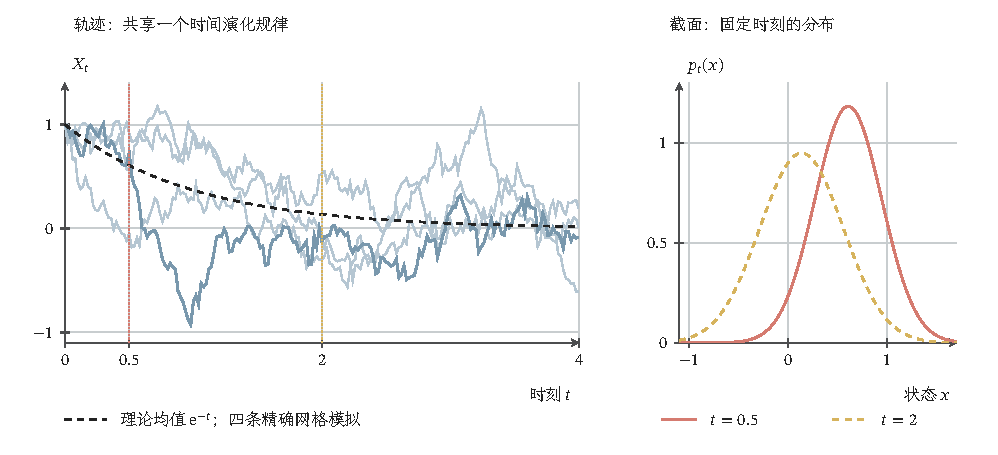
\includegraphics[width=\linewidth]{figures/01-mathematical-preliminaries/05-dynamical-systems-control-decision-and-games/tikz/dynamics/ou-paths-sections.pdf}
 \caption{OU模型的路径与截面。取$\lambda=1,\sigma=0.6,X_0=1$，
 左侧为按精确高斯转移生成的四条网格轨迹与理论均值，右侧为$t=0.5,2$
 的解析边缘密度。折线只连接模拟网格点，不是可微的连续样本路径。
 截面给出单时刻概率，时间间的相关性还由共同噪声与转移决定。}
 \label{fig:action-state-ou-paths}
\end{figure*}

\subsection{随机状态的分布演化}

逐路径的积分式不一定最适合回答“某时刻落在何处”的概率问题。
线性模型可传播少量矩，一般模型则要传播分布对测试函数的作用。
两者都来自同一演化规律，但矩摘要只有在附加分布条件下才是完整描述。

\subsubsection{线性演化下的均值与协方差}

对式~\eqref{eq:action-state-linear-sde-solution}，记
$\bm m_t=\mathbb E\bm X_t,\bm P_t=\operatorname{Cov}(\bm X_t)$。
随机积分为零均值、与初值独立，故
\begin{align*}
 \bm m_t&=\bm\Phi(t,0)\bm m_0+\int_0^t\bm\Phi(t,s)\bm c_s\,\mathrm ds,\\
 \bm P_t&=\bm\Phi(t,0)\bm P_0\bm\Phi(t,0)^\top
       +\int_0^t\bm\Phi(t,s)\bm G_s\bm G_s^\top\bm\Phi(t,s)^\top\,\mathrm ds.
\end{align*}
这里积分中的$\bm G_s\bm G_s^\top$是确定性矩阵。若扩散系数也随机，
就不能直接沿用这组确定性协方差公式；即使均方可积，取期望时也须保留
扩散系数的随机性及其与状态的关系。
两式绝对连续，对几乎处处的$t$有
\begin{align}
 \dot{\bm m}_t&=\bm A_t\bm m_t+\bm c_t,
       \label{eq:dynamical-linear-sde-mean}\\
 \dot{\bm P}_t&=\bm A_t\bm P_t+\bm P_t\bm A_t^\top+\bm G_t\bm G_t^\top.
       \label{eq:dynamical-linear-sde-covariance}
\end{align}
也可令$\widetilde{\bm X}=\bm X-\bm m$，直接用乘积Itô公式得到
\[
 \begin{split}
 \mathrm d(\widetilde{\bm X}\widetilde{\bm X}^{\top})
  ={}&(\bm A\widetilde{\bm X}\widetilde{\bm X}^{\top}
      +\widetilde{\bm X}\widetilde{\bm X}^{\top}\bm A^\top
      +\bm G\bm G^\top)\,\mathrm dt\\
    &+\bm G\,\mathrm d\bm W\,\widetilde{\bm X}^\top
      +\widetilde{\bm X}\,\mathrm d\bm W^\top\bm G^\top .
 \end{split}
\]
二阶矩界使随机积分取期望后消失，得到相同结论。
漂移传播已有不确定性，$\bm G\bm G^\top$持续注入新的不确定性；
后面的离散预测也有同样两项。

OU过程的初值只需平方可积并独立于驱动，就有
\begin{align}
 \mathbb E X_t&=\mathrm e^{-\lambda t}\mathbb E X_0,
       \label{eq:dynamical-ou-mean}\\
 \operatorname{Var}(X_t)&=\mathrm e^{-2\lambda t}\operatorname{Var}(X_0)
       +\frac{\sigma^2}{2\lambda}(1-\mathrm e^{-2\lambda t}).
       \label{eq:dynamical-ou-variance}
\end{align}
均值衰减而方差不消失。对$f(x)=x^2$换元可再次核对：
$\mathrm d(X_t^2)=(-2\lambda X_t^2+\sigma^2)\,\mathrm dt
                 +2\sigma X_t\,\mathrm dW_t$。
若漏掉$\sigma^2\,\mathrm dt$，便会错误地认为持续噪声不留下方差。
当初始分布取$\mathcal N(0,\sigma^2/(2\lambda))$时，OU过程平稳；
一般初态只是在长期趋于该分布，而非每条路径趋于零。
$\sigma=0$时稳态退化为$\delta_0$。非高斯初值的有限时刻分布通常仍非高斯，
上面两个矩不能单独确定它。

\subsubsection{一般演化下的分布与密度}

设确定性系数与适当的解唯一性使$\bm X$成为Markov过程。
要知道分布怎样变化，可先观察任意光滑“读数”$\varphi(\bm X_t)$的短时期望。
\begin{definition}[Itô扩散的生成元]
 \label{def:dynamical-diffusion-generator}
 记$\mathbb E_{t,\bm x}$为从时刻$t$的状态$\bm x$出发的期望。
 对属于算子定义域的测试函数，生成元定义为
 \[
  (\mathcal L_t\varphi)(\bm x)
    =\lim_{h\downarrow0}
       \frac{\mathbb E_{t,\bm x}\varphi(\bm X_{t+h})-\varphi(\bm x)}h.
 \]
 对连续系数的扩散，令$\bm a=\bm\sigma\bm\sigma^\top$；
 在极限与期望可交换时，Itô公式给出
 \[
  \mathcal L_t\varphi=\bm b^\top\nabla\varphi+
                      \tfrac12\operatorname{tr}(\bm a\nabla^2\varphi).
 \]
\end{definition}
从积分Itô公式取条件期望，除以$h$再令$h\downarrow0$，即得最后一式。
例如取光滑紧支撑$\varphi$，并使系数在相关区域有界，可以先局部化来核对该极限。
若时间系数仅可测，则优先使用下面的积分弱式，不强求每个时刻的点态极限。

写$\mu_t$为状态分布。在鞅项可积且均值为零时，
\[
 \int\varphi\,\mathrm d\mu_t-\int\varphi\,\mathrm d\mu_0
     =\int_0^t\int\mathcal L_s\varphi\,\mathrm d\mu_s\,\mathrm ds.
\]
这是不要求密度存在的弱演化式。对有限活动的原计数驱动，还须加上
$\lambda[\varphi(\bm x+\bm\gamma(t,\bm x))-\varphi(\bm x)]$；
若方程用补偿驱动，则漂移算子相应增加
$\lambda[\varphi(\bm x+\bm\gamma)-\varphi(\bm x)
                          -\nabla\varphi^\top\bm\gamma]$。
离散跳跃由有限差算子表达，不是无条件多加一个扩散Hessian项。

若$\mu_t$有密度$p(t,\bm x)$，代入扩散弱式，漂移项分部积分一次，
扩散项分部积分两次，得到
\begin{align*}
 \int\varphi\,\partial_t p\,\mathrm d\bm x
  &=\int\left[\sum_i b_i\partial_i\varphi
            +\tfrac12\sum_{i,j}a_{i,j}\partial_{i,j}\varphi\right]p\,\mathrm d\bm x\\
  &=\int\varphi\left[-\sum_i\partial_i(b_ip)
           +\tfrac12\sum_{i,j}\partial_i\partial_j(a_{i,j}p)\right]\,\mathrm d\bm x .
\end{align*}
测试函数紧支撑时无无穷远边界项；有界区域还需与模型匹配的边界条件。
因此得到\term{Fokker--Planck方程}
\begin{equation}
 \partial_t p=-\sum_i\partial_i(b_ip)
                  +\tfrac12\sum_{i,j}\partial_i\partial_j(a_{i,j}p).
 \label{eq:dynamical-fokker-planck}
\end{equation}
弱等式先成立；经典逐点形式另需$p$和系数的时间、空间正则性。
例如全空间光滑有界系数与一致椭圆扩散是获得正时间光滑密度的一组常用充分条件。
这里一致椭圆（uniformly elliptic）指存在固定$c>0$，使所讨论的时间与状态范围内，
\[
 \bm v^\top\bm a(t,\bm x)\bm v\geq c\|\bm v\|_2^2
 \quad\text{对所有 }\bm v\in\mathbb R^d\text{成立}.
\]
也就是每个方向的噪声强度都有同一个正下界。这比每个$(t,\bm x)$处分别正定更强：后者仍允许最小特征值随状态或时间趋于零。
退化扩散可能把概率留在低维集合，不能预先假定全维光滑密度。

把密度方程写成$\partial_t p=-\nabla\cdot\bm J$，其中
$J_i=b_ip-\frac12\sum_j\partial_j(a_{i,j}p)$。
在$p>0$处，令$\bm v=\bm J/p$，便得到概率流速度
\begin{equation}
 \bm v(t,\bm x)=\bm b(t,\bm x)
   -\tfrac12[\operatorname{div}\bm a(t,\bm x)
                         +\bm a(t,\bm x)\nabla_{\bm x}\log p(t,\bm x)],
 \quad
 (\operatorname{div}\bm a)_i=\sum_j\partial_j a_{i,j}.
 \label{eq:action-state-probability-flow}
\end{equation}
式中的$\bm s_t(\bm x)=\nabla_{\bm x}\log p(t,\bm x)$称为状态密度分数
（state score），表示在状态空间中对数密度上升最快的局部方向。
它对状态$\bm x$求导；前面统计几何中的参数得分对模型参数求导，两者的自变量及向量维数通常不同。
例如OU过程某个时刻的边缘为$\mathcal N(m_t,v_t)$且$v_t>0$时，
$s_t(x)=-(x-m_t)/v_t$，直接指向密度中心，距中心越远时幅度越大。
若此速度的ODE流存在、连续性方程适定，并具有同样初始密度及边界通量，
它便传播同样的边缘密度。只有$\bm a$不依赖状态时，散度项才消失。
流匹配不是路径匹配：ODE在给定初态后无新的噪声，而扩散不断注入随机增量。

时间反演也不是把$b$单独取负。固定终点$T$，用正向反演时钟$s$定义
$\widehat{\bm X}_s=\bm X_{T-s}$。在正密度、系数和密度足够光滑、
扩散非退化及相应可积条件下，其反演滤过中的扩散矩阵为$\bm a(T-s,\bm x)$，
漂移为
\[
 \widehat{\bm b}(s,\bm x)
    =-\bm b(T-s,\bm x)+\operatorname{div}\bm a(T-s,\bm x)
                  +\bm a(T-s,\bm x)\nabla_{\bm x}\log p(T-s,\bm x).
\]
例如可先在远离奇异端点的紧时间区间上取光滑有界系数、一致椭圆矩阵、
正的光滑密度及局部可积的分数，并另保证反演方程无爆炸。
反演Brownian运动相对于反演历史定义，不能当作原Brownian路径简单反号。
这一结果还用到正反向转移的Bayes关系；前向密度方程本身不确定时间间联合规律。
在生成模型中用估计分数替换真实分数，会再引入模型误差。

\subsection{随机轨迹的模拟与采样}

有限时域模拟问数值状态是否接近给定随机模型；长期采样问所构造的链是否按目标
分布取样。前一问题可以比较耦合路径或测试函数，后一问题还要检查不变性、遍历性
和混合速度。两者都使用随机数，但保证的对象不同。

\subsubsection{有限时域的轨迹模拟}

固定$T$，取$t_k=kh$、$n=T/h$为整数，初值
$\widehat{\bm X}_0=\bm X_0$。Euler--Maruyama方法冻结每段左端的系数：
\begin{equation}
 \widehat{\bm X}_{k+1}=\widehat{\bm X}_k+
    h\bm b(t_k,\widehat{\bm X}_k)
    +\bm\sigma(t_k,\widehat{\bm X}_k)\sqrt h\,\bm\varepsilon_k,
 \qquad \bm\varepsilon_k\overset{\mathrm{iid}}{\sim}\mathcal N(\bm0,\bm I_m).
 \label{eq:dynamical-euler-maruyama}
\end{equation}
新噪声与初值、先前噪声独立。扩散项乘$\sqrt h$，才能每单位时间累计有限方差；
随机逼近中的步长乘观测误差通常是$h\xi_k$，方差尺度为$h^2$，两者不是同一极限。

Poisson驱动须另生成$\Delta N_k\sim\operatorname{Pois}(\lambda h)$，
并按驱动假设与Brownian增量独立。网格法用
$\bm\gamma(t_k,\widehat{\bm X}_k)\Delta N_k$冻结该段跳幅；
补偿版本改用$\Delta N_k-\lambda h$。当一段内有多个事件且跳幅依赖状态时，
这种冻结不同于逐事件更新。
事件适配法则依次采样独立$\operatorname{Exp}(\lambda)$等待时间，
把跳时插入网格，在事件间模拟扩散、在事件处用跳前状态更新。
这里Brownian增量仍按各段实际长度采样，不能用高斯增量冒充跳跃计数。

\paragraph{同一噪声下的状态误差}

强误差必须把算法和真解放在同一个驱动上，即令
$\sqrt h\,\bm\varepsilon_k=\bm W_{t_{k+1}}-\bm W_{t_k}$。
对自治系数，在全局Lipschitz、线性增长和$\bm X_0\in L^2$条件下，
固定有限时域有
\[
 \max_{0\leq k\leq n}
   \bigl(\mathbb E\|\bm X_{t_k}-\widehat{\bm X}_k\|^2\bigr)^{1/2}
     \leq C_T h^{1/2}.
\]
显式时间依赖时，一组充分条件是统一状态Lipschitz，并有
$\|\bm b(t,\bm x)-\bm b(s,\bm x)\|
 +\|\bm\sigma(t,\bm x)-\bm\sigma(s,\bm x)\|_{\mathrm F}
 \leq K(1+\|\bm x\|)|t-s|^{1/2}$。
常数依赖$T$和系数界，不是无限时域的统一保证。

估计机制与存在性证明相连。定义连续插值
\[
 \begin{split}
 \widehat{\bm X}_t={}&\bm X_0+
    \int_0^t\bm b(\eta(s),\widehat{\bm X}_{\eta(s)})\,\mathrm ds\\
 &+\int_0^t\bm\sigma(\eta(s),\widehat{\bm X}_{\eta(s)})\,\mathrm d\bm W_s,
 \end{split}
\]
其中$\eta(s)=t_{\lfloor s/h\rfloor}$，插值在网格上等于算法值。
增长界先给出统一二阶矩，并由等距得到
$\sup_{s\leq T}\mathbb E\|\widehat{\bm X}_s-\widehat{\bm X}_{\eta(s)}\|^2
\leq C_T h$。相减积分方程，用Lipschitz、最大不等式和时间正则性得
\[
 E(t):=\mathbb E\sup_{r\leq t}\|\bm X_r-\widehat{\bm X}_r\|^2
       \leq C_T\int_0^tE(s)\,\mathrm ds+C_T h.
\]
Grönwall给出$E(T)\leq C'_T h$，开方即得强半阶。
加性噪声等结构可能提高阶数，但不是一般乘性噪声的保证；
跳跃扩展还需另核对跳幅、驱动耦合与事件处理。

\paragraph{测试函数下的期望误差}

弱误差不逐路径相减，而是比较读数的期望。一组方便的自治充分条件是漂移、
扩散与测试函数$\varphi$具有至四阶连续有界导数，并满足增长和所需矩条件；
更保守地可取它们本身及至四阶导数均有界。此时
\[
  |\mathbb E\varphi(\bm X_T)-\mathbb E\varphi(\widehat{\bm X}_n)|
        \leq C_{\varphi,T}h.
\]
其机制是对剩余期望函数
$u(t,\bm x)=\mathbb E_{t,\bm x}\varphi(\bm X_T)$作局部展开。
在其相应导数有界的条件下，精确转移与一次Euler转移都给出
$u+h\mathcal L u+O(h^2)$。把每步的期望差望远镜相加，
$n=T/h$个局部$O(h^2)$误差累计为$O(h)$。
这里引用标准弱收敛结果，导数与矩条件用于保证展开余项统一可积；
不能仅凭二阶矩和状态Lipschitz就断言弱一阶。\scite{math-kloeden1992numerical-sde}

弱阶较高不说明两条样本轨迹更接近。例如独立生成的两个同分布终点对所有可积
测试函数期望完全相同，彼此状态距离却不为零。有限时间弱误差还不能直接交换
$h\downarrow0$与$T\uparrow\infty$，长期步长偏差必须单独分析。

\subsubsection{目标分布下的长期采样}

设目标密度$\pi>0$光滑且可归一化。过阻尼Langevin模型为
\begin{equation}
 \mathrm d\bm X_t=\tfrac12\nabla\log\pi(\bm X_t)\,\mathrm dt+\mathrm d\bm W_t.
 \label{eq:dynamical-langevin-sde}
\end{equation}
代入Fokker--Planck通量，$\bm b\pi-\nabla\pi/2=\bm0$。
在方程无爆炸、边界通量为零及密度方程适定等条件下，这证明$\pi$不变。
从其他初态收敛还需遍历条件；例如$\pi\propto\mathrm e^{-U}$，
$U$光滑强凸且梯度全局Lipschitz时，噪声非退化与向内漂移提供常用保证。
多峰势能可能保持同一目标却混合很慢。

即使连续模型正确，离散化也会改变稳态。取$\pi=\mathcal N(0,1)$，
则$X_{k+1}=(1-h/2)X_k+\sqrt h\,\varepsilon_k$。
只有$0<h<4$时这一递推稳定，其稳态方差为
\[
  \frac{h}{1-(1-h/2)^2}=\frac1{1-h/4},
\]
并非$1$。减小步长减小偏差，但在相同计算步数下也缩短模拟时间；
有限预算须同时考虑初态遗留、相关性和离散误差。

Hamilton蒙特卡洛（HMC）使用另一种构造。若
$\pi(\bm q)\propto\exp[-U(\bm q)]$，引入独立
$\bm p\sim\mathcal N(\bm0,\bm M)$，联合密度为
$\rho(\bm q,\bm p)\propto\exp[-H(\bm q,\bm p)]$。
精确Hamilton流保持能量和体积，因此保持$\rho$；
蛙跳只保持体积与可逆结构，需要接受校正补偿能量误差。
固定步长$h$与步数$L$，记$T=R\circ\Psi_h^L$，
其中$R(\bm q,\bm p)=(\bm q,-\bm p)$。
前面已证明$R\Psi_hR=\Psi_h^{-1}$，故$T^2=I$，且$|\det DT|=1$。
对$\bm z' =T\bm z$，接受概率取
\begin{equation}
 \alpha(\bm z)=\min\{1,\exp[-H(\bm z')+H(\bm z)]\}.
 \label{eq:dynamical-hmc-acceptance}
\end{equation}

\begin{theorem}[HMC提议的详细平衡]
 \label{thm:action-state-hmc-balance}
 若$T$是可微、体积保持的对合，则以概率$\alpha(\bm z)$移至$T\bm z$，
 否则留在$\bm z$的核，对密度$\rho$满足详细平衡。
\end{theorem}
\begin{proof}
 接受部分的密度权重为
 $\rho(\bm z)\alpha(\bm z)=\min\{\rho(\bm z),\rho(T\bm z)\}$。
 对任意有界可测函数$g(\bm z,\bm z')$，作变量替换$\bm y=T\bm z$，
 由$T^2=I$和单位绝对Jacobian，
 \[
 \begin{split}
 &\int g(\bm z,T\bm z)\min\{\rho(\bm z),\rho(T\bm z)\}\,\mathrm d\bm z\\
 &\quad=\int g(T\bm y,\bm y)
                   \min\{\rho(T\bm y),\rho(\bm y)\}\,\mathrm d\bm y .
 \end{split}
 \]
 这证明接受部分在交换出发与到达状态后不变。
 拒绝部分集中在对角线$\bm z'=\bm z$，本身对称，两者相加即为详细平衡。
\end{proof}

一轮算法因而是：保留当前位置并重新抽取高斯动量；按三子步蛙跳执行$L$次；
翻转末端动量并计算$\Delta H$；抽取独立均匀数，按
$\min(1,\mathrm e^{-\Delta H})$接受，否则保留原位置。
动量刷新是联合目标的条件抽样，保持$\rho$；再接上述核仍保持$\rho$，
边缘化动量得到位置目标$\pi$。两个保持核的复合不必在联合空间仍可逆，
此处不把复合的不变性误说成自动详细平衡。

若提议不保持体积，接受比还需Jacobian因子；状态依赖地改变步数或步长，
也须重新核对反向提议。实现中的有限精度可逆误差不是上述精确算术证明的一部分。
接受校正不保证独立样本或快速混合：步长过大导致拒绝，轨迹过短导致高相关，
质量矩阵失配使不同方向移动不均衡。采样以保持分布为目标，不要求能量一路下降，
所以不能将Hamilton轨迹解释为更快的梯度下降。

\begin{table*}[htbp]
 \centering
 \begin{tabularx}{\linewidth}{lXX}
 \toprule
 结论 & 所比较的对象 & 尚未得到的保证\\
 \midrule
 强数值误差小 & 同一驱动下数值状态与真状态 & 长期抽样偏差小\\
 弱数值误差小 & 两种状态分布的测试函数期望 & 单条路径距离小\\
 密度$\pi$不变 & 从$\pi$出发仍保持$\pi$ & 其他初态快速趋于$\pi$\\
 概率流匹配边缘 & 每个时刻的状态分布 & 相同时间间联合规律\\
 \bottomrule
 \end{tabularx}
 \caption{随机演化中几种保证的对象。每一项均依赖当地给出的正则、边界或数值条件，
 不能用一个对象上的结论替代另一个对象上的结论。}
 \label{tab:dynamical-path-distribution}
\end{table*}

\section{随机状态的观测与推断}
\label{sec:dynamical-state-space-filtering}
\label{sec:dynamical-stochastic-state-observation}

过程噪声规定真实状态如何随机移动；传感器读数则提供关于这条未知轨迹的证据。
因此推断不是再次生成一条任意轨迹，而是在已给定的生成模型中，保留与读数相容的
状态并重新分配概率。先明确可见数据与查询目标，再把预测、滤波和平滑化为可计算公式。

\subsection{状态观测与推断目标}

在前面的状态转移$K_t$之外增加观测核
$G_t(\bm x,B)=\mathbb P(\bm y_t\in B\mid\bm x_t=\bm x)$。
它表示状态为$\bm x$时传感器返回哪些读数。线性加性例为
\begin{equation}
  \bm y_t=\bm C_t\bm x_t+\bm v_t.
  \label{eq:dynamical-linear-observation-model}
\end{equation}
先假设初值、所有过程噪声与所有观测噪声相互独立，输入与矩阵给定。
于是给定$\bm x_t$后，$\bm y_t$不再依赖旧状态和旧观测；
给定当前状态后，下一状态由$K_t$生成。联合规律在
式~\eqref{eq:dynamical-linear-state-model}的基础上分解为
\[
 \pi_0(\mathrm d\bm x_0)
       \prod_{t=0}^{T-1}K_t(\bm x_t,\mathrm d\bm x_{t+1})
       \prod_{t=1}^T G_t(\bm x_t,\mathrm d\bm y_t).
\]
这里从$y_1$开始观察，$\pi_0$不含一个未声明的$y_0$。
若噪声相关、传感器依赖旧状态或有内部滞后，须扩充联合状态或显式改写这些
条件关系。观测序列通常不满足自身的Markov性，因为一次带噪读数未必概括隐藏状态。

记$\mathcal Y_t=\sigma(\bm y_1,\ldots,\bm y_t)$，
$\mathcal Y_0$为无观测信息。欧氏状态与观测具有正则条件分布，
使“给定这段读数的状态概率”能作为概率核处理。
即使观测无噪，也不一定足够：$y_t=x_{1,t}+x_{2,t}$不能区分
$(1,0)^\top$与$(0,1)^\top$。能否借后续动力学区分这些方向，需要
第~\ref{chap:control-theory}章的可观测性与可检测性条件。

\begin{example}[带泄漏温度的间接观测]
 \label{ex:dynamical-noisy-temperature}
 回到同一模型
 $x_{t+1}=0.8x_t+u_t+w_{t+1}$、$y_t=x_t+v_t$，
 其中$w_t\sim\mathcal N(0,0.04)$、$v_t\sim\mathcal N(0,0.09)$，
 与初值及彼此独立。即使传感器完全精确，未来仍因$w_{t+1}$不确定；
 即使过程无噪，当前状态也可能因读数噪声而不确定。
 图~\ref{fig:action-state-temperature-layers}的轨迹从已知$x_0=0$出发，
 使用给定$u_t=0.4$；后面的估计继续使用该初值与同一组读数，
 不另换一条更利于展示的状态轨迹。
\end{example}

得到条件分布后，还须规定输出什么估计。平方损失下，若$\bm X$二阶可积，
对信息$\mathcal G$可测的估计$\bm a$，
\[
 \mathbb E[\|\bm X-\bm a\|^2\mid\mathcal G]
 =\mathbb E[\|\bm X-\mathbb E(\bm X\mid\mathcal G)\|^2\mid\mathcal G]
       +\|\mathbb E(\bm X\mid\mathcal G)-\bm a\|^2.
\]
交叉项因条件均值为零而消失，所以条件均值最小化均方损失。
离散状态的零一损失选条件众数；连续密度的MAP是另一种点输出，
不能不说明损失就把所有“最优估计”视为同义。

\subsection{不同观测范围下的边缘状态推断}
\label{sec:dynamical-kalman-rts}

固定目标时刻$t$，改变可用观测的终点$j$。记
$\bm m_{t\mid j}=\mathbb E[\bm x_t\mid\mathcal Y_j]$、
$\bm P_{t\mid j}=\operatorname{Cov}(\bm x_t\mid\mathcal Y_j)$。
三种查询的区别先由信息范围决定，与使用哪一种算法无关。

\begin{table}[htbp]
 \centering
 \begin{tabularx}{\linewidth}{lXX}
 \toprule
 查询 & 目标条件分布 & 允许的观测\\
 \midrule
 一步预测 & $P(\bm x_t\mid\mathcal Y_{t-1})$ & 新读数以前\\
 当前滤波 & $P(\bm x_t\mid\mathcal Y_t)$ & 包括当前读数\\
 固定区间平滑 & $P(\bm x_t\mid\mathcal Y_T)$，$T>t$ & 包括事后未来读数\\
 \bottomrule
 \end{tabularx}
 \caption{同一目标状态的三种边缘查询。信息终点改变，物理状态并未改变；
 平滑使用的未来读数不能用于当时的在线行动。}
 \label{tab:dynamical-estimation-information}
\end{table}

下面的一般核公式只要求前述条件独立结构。需要解析闭合时，再采用有限时域
线性高斯条件：
\[
 \bm x_0\sim\mathcal N(\bm m_{0\mid0},\bm P_{0\mid0}),\quad
 \bm w_{t+1}\sim\mathcal N(\bm0,\bm Q_{t+1}),\quad
 \bm v_t\sim\mathcal N(\bm0,\bm R_t).
\]
三组随机量彼此独立，系统矩阵与输入确定，
$\bm P_{0\mid0},\bm Q_{t+1}\succeq\bm0$，先取$\bm R_t\succ\bm0$。
本章统一让$w_{t+1}$与它推动到达的状态时刻一致；
因此从$t-1$到$t$的过程协方差写为$\bm Q_t$。
这些条件在每个有限$T$内使用，不预设滤波增益已达稳态。

\subsubsection{过去观测下的状态预测}

若已有截至$t-1$的条件分布$\pi_{t-1}$，全概率公式给出
\begin{equation}
 \pi_{t\mid t-1}(A)
     =\int K_{t-1}(\bm x,A)\,\pi_{t-1}(\mathrm d\bm x).
 \label{eq:dynamical-general-prediction-kernel}
\end{equation}
这是把每个候选旧状态的下一步分布，按其当前可信程度混合。
多步预测重复施加转移核，中途没有新观测便没有似然校正。

例如隐藏状态为$\{0,1\}$，$\pi_0=(0.7,0.3)$，
按当前状态为行、下一状态为列的转移矩阵为
$\bm P=\left[\begin{smallmatrix}0.8&0.2\\0.1&0.9\end{smallmatrix}\right]$。
于是$\pi_{1\mid0}(1)=0.7(0.2)+0.3(0.9)=0.41$，
$\pi_{1\mid0}(0)=0.59$。这是尚未看$y_1$的结果；
下一小节再用同一预测做校正。

在线性高斯条件下，仿射变换与独立高斯相加保持高斯性，所以
\begin{align}
 \bm m_{t\mid t-1}
   &=\bm A_{t-1}\bm m_{t-1\mid t-1}+\bm B_{t-1}\bm u_{t-1},
       \label{eq:dynamical-kalman-predicted-mean}\\
 \bm P_{t\mid t-1}
   &=\bm A_{t-1}\bm P_{t-1\mid t-1}\bm A_{t-1}^\top+\bm Q_t.
       \label{eq:dynamical-kalman-predicted-covariance}
\end{align}
温度第一步为$m_{1\mid0}=0.4,P_{1\mid0}=0.04$：
初值已知并不等于未来状态已知。一般预测方差并非必然大于旧方差，
因为$\bm A$可能收缩；过程噪声是在已传播的协方差之上增加$\bm Q_t$。
若$w_t$与旧状态相关，须增加
$\bm A_{t-1}\operatorname{Cov}(\bm x_{t-1},\bm w_t\mid\mathcal Y_{t-1})$
及其转置，并使用噪声的条件均值和条件协方差。
未经核对独立性就删交叉项，会改变预测。

\subsubsection{当前及过去观测下的状态滤波}

\begin{definition}[滤波分布]
 \label{def:dynamical-filtering-distribution}
 当前状态在截至当前的观测信息下的条件概率核
 \begin{equation}
  \pi_t(A)=\mathbb P(\bm x_t\in A\mid\mathcal Y_t)
   \label{eq:dynamical-filtering-distribution}
 \end{equation}
 称为\term{滤波分布}。它与真实状态$\bm x_t$、实际读数$\bm y_t$分别是
 推断结果、潜在对象与数据。
\end{definition}

若观测核有相对于共同$\sigma$有限测度$\nu_t$的联合可测密度
$G_t(\bm x,\mathrm d\bm y)=g_t(\bm y\mid\bm x)\nu_t(\mathrm d\bm y)$，
则Bayes公式给出
\begin{equation}
 \pi_t(\mathrm d\bm x)=
 \frac{g_t(\bm y_t\mid\bm x)\pi_{t\mid t-1}(\mathrm d\bm x)}
      {\int g_t(\bm y_t\mid\bm z)\pi_{t\mid t-1}(\mathrm d\bm z)}.
 \label{eq:dynamical-general-bayes-filter}
\end{equation}
分母必须有限且严格为正。共同支配测度不依赖候选状态，才能把这些似然放在同一
尺度比较；没有这种密度表示时仍有正则条件分布，但不能生搬该比值。

\begin{example}[两状态模型的一次预测与校正]
 \label{ex:dynamical-two-state-bayes-filter}
 接续上一小节的预测结果。若
 $\mathbb P(y_1=1\mid x_1=0)=0.2$、
 $\mathbb P(y_1=1\mid x_1=1)=0.8$，实际看到$y_1=1$后，
 \[
  \pi_1(1)=\frac{0.8(0.41)}{0.2(0.59)+0.8(0.41)}
              =\frac{164}{223}\approx0.735.
 \]
 新证据使状态$1$的相对权重上升。只需$\pi_0$而不重新读取更早观测，
 是因为条件独立结构已经把过去对未来有用的信息压入该分布。
\end{example}

在线性高斯模型中，上面的密度乘积可以用一次联合高斯条件化完成。
给定$\mathcal Y_{t-1}$，
\begin{equation}
 \begin{bmatrix}\bm x_t\\\bm y_t\end{bmatrix}
 \sim\mathcal N\left(
 \begin{bmatrix}\bm m_{t\mid t-1}\\\bm C_t\bm m_{t\mid t-1}\end{bmatrix},
 \begin{bmatrix}
  \bm P_{t\mid t-1}&\bm P_{t\mid t-1}\bm C_t^\top\\
  \bm C_t\bm P_{t\mid t-1}&\bm S_t
 \end{bmatrix}\right),
 \label{eq:dynamical-kalman-joint-gaussian}
\end{equation}
其中\term{创新协方差}为
\begin{equation}
 \bm S_t=\bm C_t\bm P_{t\mid t-1}\bm C_t^\top+\bm R_t.
 \label{eq:dynamical-kalman-innovation-covariance}
\end{equation}
创新$\bm r_t=\bm y_t-\bm C_t\bm m_{t\mid t-1}$是读数超出预测观测的部分。
$\bm R_t\succ\bm0$保证$\bm S_t$可逆。由条件高斯公式，
\begin{align}
 \bm K_t&=\bm P_{t\mid t-1}\bm C_t^\top\bm S_t^{-1},
       \label{eq:dynamical-kalman-gain}\\
 \bm m_{t\mid t}&=\bm m_{t\mid t-1}+\bm K_t\bm r_t,
       \label{eq:dynamical-kalman-filtered-mean}\\
 \bm P_{t\mid t}&=\bm P_{t\mid t-1}-\bm K_t\bm S_t\bm K_t^\top.
       \label{eq:dynamical-kalman-filtered-covariance}
\end{align}
Kalman增益$\bm K_t$由两类误差协方差决定，不是自由设置的学习率。
减去的是半正定项，所以这次高斯校正不增加条件协方差。
一般非高斯模型中，“更多信息减少均方误差”是平均意义的结论，
不保证每个罕见读数对应的后验方差都比先验小。\scite{math-kalman1960filtering}

\begin{theorem}[有限时域Kalman滤波]
 \label{thm:dynamical-finite-horizon-kalman-filter}
 在上述独立线性高斯模型与创新协方差可逆条件下，预测与校正公式精确给出
 $\bm x_t\mid\mathcal Y_t\sim
       \mathcal N(\bm m_{t\mid t},\bm P_{t\mid t})$，对每个有限$t$成立。
\end{theorem}
\begin{proof}
 $t=0$时无观测，条件分布就是给定高斯初值。假设上一时刻结论成立，
 独立高斯过程噪声与线性状态更新得到式
 ~\eqref{eq:dynamical-kalman-predicted-mean}和
 ~\eqref{eq:dynamical-kalman-predicted-covariance}，并保持高斯性。
 独立高斯观测噪声又给出式~\eqref{eq:dynamical-kalman-joint-gaussian}。
 为核对条件化，令$\bm e=\bm x_t-\bm m_{t\mid t-1}-\bm K_t\bm r_t$。
 在$\mathcal Y_{t-1}$条件下，
 $\operatorname{Cov}(\bm e,\bm r_t)
   =\bm P_{t\mid t-1}\bm C_t^\top-\bm K_t\bm S_t=\bm0$。
 联合高斯中不相关即独立，所以给定新读数后$\bm e$仍为零均值高斯，
 协方差为$\bm P_{t\mid t-1}-\bm K_t\bm S_t\bm K_t^\top$。
 新条件均值与协方差正是上述校正式，归纳完成。
\end{proof}

把估计误差写成
$(\bm I-\bm K_t\bm C_t)(\bm x_t-\bm m_{t\mid t-1})-\bm K_t\bm v_t$，
利用两项误差独立，得到Joseph形式
\begin{equation}
 \bm P_{t\mid t}=(\bm I-\bm K_t\bm C_t)\bm P_{t\mid t-1}
                    (\bm I-\bm K_t\bm C_t)^\top+\bm K_t\bm R_t\bm K_t^\top.
 \label{eq:dynamical-kalman-joseph-form}
\end{equation}
展开并用$\bm K_t\bm S_t=\bm P_{t\mid t-1}\bm C_t^\top$，
即恢复简化校正式。半正定项相加的形式更利于有限精度下维持协方差性质；
实现应解线性方程求增益作用，不显式形成$\bm S_t^{-1}$。

\begin{example}[标量观测怎样权衡预测与读数]
 \label{ex:dynamical-scalar-kalman-update}
 对$y=x+v$、$v\sim\mathcal N(0,r)$，有
 $K=p^-/(p^-+r)$、$m^+=m^-+K(y-m^-)$、$p^+=p^-r/(p^-+r)$。
 独立任务例取$(m^-,p^-,r,y)=(0,4,1,2)$，得到
 $K=4/5,m^+=8/5,p^+=4/5$。
 温度模型则仍用$r=0.09$，第一步增益为$0.04/0.13=4/13$，
 $m_{1\mid1}=0.4+\frac4{13}(y_1-0.4)$、
 $P_{1\mid1}=0.036/1.3\approx0.02769$。
 两例用于比较同一公式，不能互换噪声参数。
\end{example}

观测越精确，直接观测方向的增益通常越大；未被$\bm C_t$区分的方向可能仍有
不确定性。图~\ref{fig:dynamical-kalman-density-update}显示标量分布如何重加权：
密度变高表示质量集中，不是单点概率大于$1$。
\begin{figure}[htbp]
 \centering
 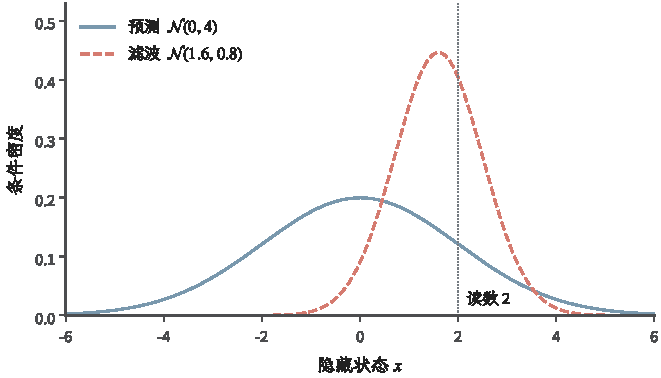
\includegraphics[width=\linewidth]{figures/01-mathematical-preliminaries/05-dynamical-systems-control-decision-and-games/matplotlib/dynamics/kalman-density-update.pdf}
 \caption{独立标量教学例的预测$\mathcal N(0,4)$与后验$\mathcal N(1.6,0.8)$，
 实际读数$y=2$、观测噪声方差$1$。第二个高斯参数是方差；
 本图不是贯穿温度模型的参数设定。}
 \label{fig:dynamical-kalman-density-update}
\end{figure}
\FloatBarrier

若状态更新为$\bm x_{t+1}=\bm f_t(\bm x_t)+\bm w_{t+1}$，
观测为$\bm y_t=\bm h_t(\bm x_t)+\bm v_t$，查询仍是同一个滤波分布，
只是高斯闭合一般失效。扩展Kalman滤波（EKF）在滤波均值附近以
$\bm F_t=D\bm f_t(\bm m_{t\mid t})$传播协方差，
预测均值取$\bm f_t(\bm m_{t\mid t})$；
在预测均值处以$\bm H_{t+1}=D\bm h_{t+1}(\bm m_{t+1\mid t})$
构造创新协方差和增益。它把局部函数替换为一阶线性函数，
所以通常既忽略曲率对均值的影响，也把后验压回单个高斯。

无迹Kalman滤波（UKF）用确定性sigma点近似非线性矩传播。
例如对$d$维均值$\bm m$与协方差$\bm P=\bm L\bm L^\top$，
取$\kappa\geq0$，点为$\bm m$及
$\bm m\pm\sqrt{d+\kappa}\bm L_{\cdot i}$，权重分别为
$\kappa/(d+\kappa)$与$1/[2(d+\kappa)]$。
它们精确匹配原均值与协方差。将点代入$\bm f$，以加权和、加权外积估计
新均值与协方差，再给协方差加上过程噪声$\bm Q$。
本处采用重新生成点的实现：依据加入$\bm Q$后的预测均值和协方差重新构造sigma点，
再把这组点送入$\bm h$，计算预测观测均值、观测协方差及状态观测交叉协方差。
观测协方差还须加上观测噪声$\bm R$，随后按Kalman的创新与增益公式校正。
重新生成点使观测预测也包含本步新增的过程不确定性。
例如标量线性系统$f(x)=h(x)=x$，旧状态方差$p=1$，过程与观测噪声方差
$q=r=1$，上述步骤给出预测方差$2$、创新方差$3$、交叉方差$2$，故增益为$2/3$，
与精确Kalman公式一致；直接复用未包含$q$的原传播点则无法得到这个结果。
这是简单的非负权重构造，实际UKF还可使用带缩放参数的不同权重。
其近似发生在矩积分和高斯投影，不是把非线性模型变成精确线性模型。

两种方法都可能遗漏多峰后验。例如零均值对称先验配上
$y=x^2+v$，一个明显正的读数可能支持正负两个状态区间。
EKF在$x=0$的观测导数为零；对称sigma点也有零状态观测交叉协方差，
单高斯校正不能表达分裂成两峰的证据。
粒子滤波改用加权经验分布$\sum_i\omega_t^{(i)}\delta_{x_t^{(i)}}$：
从已有粒子按转移核抽下一状态，将权重乘当前似然再归一化，
必要时按权重重采样。其近似对象是整个滤波概率测度，
并用有限样本替代核积分；权重集中、高维与重采样损失多样性仍是限制。
高斯混合则保留多个分量，分别传播和校正，再用似然更新分量权重；
分量合并或剪枝会引入另一种近似。

\subsubsection{有限时域完整观测下的状态平滑}

固定终点$T$后，未来读数也能帮助判断旧状态。关键不是再向前预测，
而是把新获得的下一状态分布通过反向条件关系传回去。
在线性高斯条件下，给定$\mathcal Y_t$，
\[
 \begin{bmatrix}\bm x_t\\\bm x_{t+1}\end{bmatrix}
 \sim\mathcal N\left(
 \begin{bmatrix}\bm m_{t\mid t}\\\bm m_{t+1\mid t}\end{bmatrix},
 \begin{bmatrix}
  \bm P_{t\mid t}&\bm P_{t\mid t}\bm A_t^\top\\
  \bm A_t\bm P_{t\mid t}&\bm P_{t+1\mid t}
 \end{bmatrix}\right).
\]
若$\bm P_{t+1\mid t}$可逆，条件高斯公式给出
\begin{align}
 \bm J_t&=\bm P_{t\mid t}\bm A_t^\top\bm P_{t+1\mid t}^{-1},
    \label{eq:dynamical-rts-gain}\\
 \mathbb E[\bm x_t\mid\bm x_{t+1},\mathcal Y_t]
   &=\bm m_{t\mid t}+\bm J_t(\bm x_{t+1}-\bm m_{t+1\mid t}),
    \label{eq:dynamical-rts-one-step-conditional-mean}\\
 \operatorname{Cov}(\bm x_t\mid\bm x_{t+1},\mathcal Y_t)
   &=\bm P_{t\mid t}-\bm J_t\bm P_{t+1\mid t}\bm J_t^\top.
    \label{eq:dynamical-rts-one-step-conditional-covariance}
\end{align}
这里的$\bm J_t$关联相邻状态，不是由当前传感器直接得到的Kalman增益。

\begin{theorem}[有限时域RTS平滑]
 \label{thm:dynamical-rts-smoother}
 在有限时域Kalman条件及每个$\bm P_{t+1\mid t}$可逆条件下，
 从终点$(\bm m_{T\mid T},\bm P_{T\mid T})$向后递推
 \begin{align}
  \bm m_{t\mid T}
   &=\bm m_{t\mid t}+\bm J_t(\bm m_{t+1\mid T}-\bm m_{t+1\mid t}),
       \label{eq:dynamical-rts-smoothed-mean}\\
  \bm P_{t\mid T}
   &=\bm P_{t\mid t}
         +\bm J_t(\bm P_{t+1\mid T}-\bm P_{t+1\mid t})\bm J_t^\top,
       \label{eq:dynamical-rts-smoothed-covariance}
 \end{align}
 精确给出$\bm x_t\mid\mathcal Y_T$的高斯均值与协方差。
\end{theorem}
\begin{proof}
 给定$\bm x_{t+1}$后，未来状态和观测与更早状态条件独立，因此
 $P(\mathrm d\bm x_t\mid\bm x_{t+1},\mathcal Y_T)
   =P(\mathrm d\bm x_t\mid\bm x_{t+1},\mathcal Y_t)$。
 全概率公式给出后向因子化
 \begin{equation}
  P(\mathrm d\bm x_t\mid\mathcal Y_T)
   =\int P(\mathrm d\bm x_t\mid\bm x_{t+1},\mathcal Y_t)
                   P(\mathrm d\bm x_{t+1}\mid\mathcal Y_T).
  \label{eq:dynamical-rts-backward-factorization}
 \end{equation}
 将一步条件均值对$\bm x_{t+1}\mid\mathcal Y_T$取期望，
 塔式性质得到平滑均值公式。全协方差公式分成两项：条件内协方差为
 $\bm P_{t\mid t}-\bm J_t\bm P_{t+1\mid t}\bm J_t^\top$，
 条件均值的协方差为$\bm J_t\bm P_{t+1\mid T}\bm J_t^\top$；
 相加即得平滑协方差。一步条件核的均值为仿射函数、协方差不依赖下一状态，
 与高斯下一状态混合仍为高斯。从$T$向后归纳，完成全部时刻的结论。
\end{proof}

前向保存每步滤波与预测的均值、协方差，后向依次计算$\bm J_t$及上述两式，
就是Rauch--Tung--Striebel（RTS）平滑算法。\scite{math-rauch1965smoothing}
未来观测影响过去的条件分布，不改变已经发生的物理状态。

\begin{example}[未来观测降低过去状态的不确定性]
 \label{ex:dynamical-scalar-rts-update}
 用独立随机游走例$x_1=x_0+w_1$、$y_1=x_1+v_1$，
 取$m_{0\mid0}=0,P_{0\mid0}=1,Q_1=1,R_1=2/3$且噪声独立。
 观察$y_1=2$后，$m_{1\mid0}=0,P_{1\mid0}=2$，
 $K_1=3/4,m_{1\mid1}=3/2,P_{1\mid1}=1/2$。
 于是$J_0=1/2$，$m_{0\mid1}=3/4$，
 $P_{0\mid1}=1+\frac14(\frac12-2)=5/8$。
 在时刻$0$尚不能使用这个结果；此时只有均值$0$、方差$1$的初始先验。
\end{example}

\begin{figure*}[htbp]
 \centering
 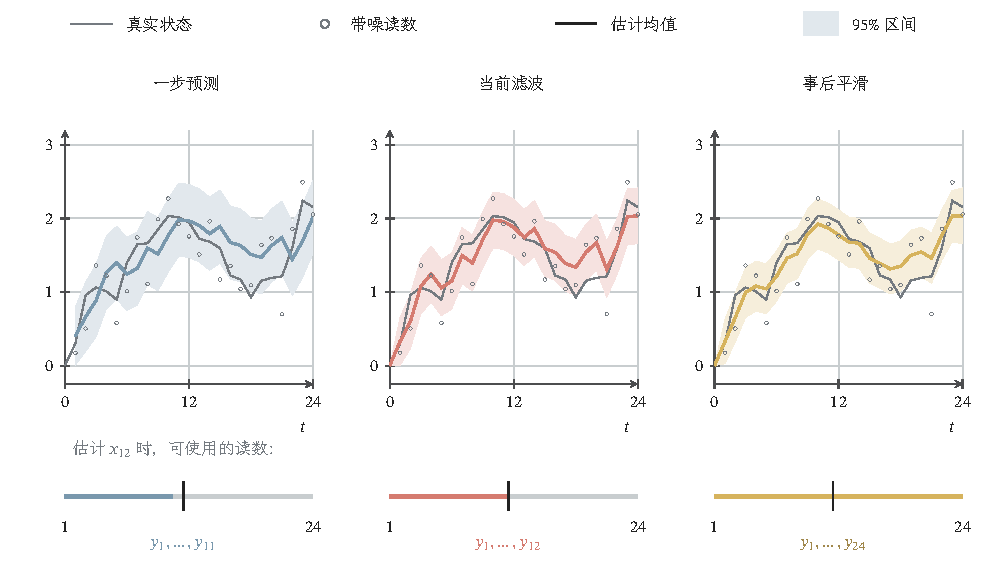
\includegraphics[width=\linewidth]{figures/01-mathematical-preliminaries/05-dynamical-systems-control-decision-and-games/tikz/dynamics/temperature-inference.pdf}
 \caption{与图~\ref{fig:action-state-temperature-layers}完全相同的温度轨迹及读数。
 三栏分别画一步预测、滤波与固定终点$T=24$的平滑均值和逐时刻$95\%$高斯区间，
 灰线为实际状态，圆点为读数；区间不是整条路径同时覆盖的置信带。
 下方以$t=12$为例标出可用观测范围。已知$x_0=0$，给定$u_t=0.4$，
 过程、观测方差仍为$0.04,0.09$。平滑的信息优势不是额外的在线能力。}
 \label{fig:action-state-temperature-inference}
\end{figure*}

图中的高斯平滑协方差不超过相应滤波协方差，但某一条实现上的均值误差不必
每个时刻都更小。条件均方误差的保证与某一次噪声实现上的误差是不同对象。
若预测协方差奇异，须在其仿射支持上条件化，广义逆只是计算工具，
还要检查条件状态是否属于支持，不能只替换逆号。
非线性近似平滑可沿相同后向关系用局部线性化或sigma点估计相邻状态的交叉矩；
粒子平滑则近似反向核或路径权重。无论采用哪种表示，使用$\mathcal Y_T$
这一信息条件都不改变。

\subsection{完整观测下的联合轨迹推断}

各时刻边缘分布回答“那一刻可能在哪里”，整条路径后验还要回答“这些状态如何
一起出现”。在共同观测密度条件下，
\begin{equation}
 P(\mathrm d\bm x_{0:T}\mid\bm y_{1:T})
   =\frac1{Z(\bm y_{1:T})}\,
      \pi_0(\mathrm d\bm x_0)
      \prod_{t=0}^{T-1}K_t(\bm x_t,\mathrm d\bm x_{t+1})
      \prod_{t=1}^Tg_t(\bm y_t\mid\bm x_t),
 \label{eq:action-state-trajectory-posterior}
\end{equation}
其中证据$Z$是分子对路径的积分，要求$0<Z<\infty$。
乘积记号按转移核的迭代积分理解，不预设状态本身有Lebesgue密度。
每个平滑边缘由这一个联合后验积分而来；反过来，只给全部边缘并不能恢复跨时刻关联。

若损失为$\sum_t\|\bm x_t-\bm a_t\|^2$，联合条件均值的各分量就是
$\bm m_{t\mid T}$，因此逐时刻平滑均值同时组成最小化该可加平方损失的路径输出。
在线性高斯模型中，把所有状态堆叠为$\bm X$后，后验仍为联合高斯。
协方差$\bm\Sigma\succ\bm0$时，其密度正比于
$\exp[-(\bm X-\bm m)^\top\bm\Sigma^{-1}(\bm X-\bm m)/2]$，
故联合众数为$\bm m$，也与各时刻的边缘众数一致。
这是一项高斯结构结论，不是所有后验的性质。

若$\bm\Sigma$奇异，后验集中在仿射支持
$\bm m+\operatorname{range}(\bm\Sigma)$，没有全维Lebesgue密度。
对$\bm\Sigma=\bm U_r\bm\Lambda_r\bm U_r^\top$，
在支持坐标$\bm z=\bm U_r^\top(\bm X-\bm m)$中才有非退化高斯密度；
其唯一众数为$\bm z=\bm0$，对应$\bm m$。
条件高斯使用广义逆时也须要求所给证据位于其支持内；
支持外的条件值属于零概率事件，公式不能赋予一个未经指定的后验意义。

非高斯下可直接看出区别。设两个时刻的联合后验为
\[
 \begin{aligned}
  P(x_0=0,x_1=0)&=0.40,\\
  P(x_0=0,x_1=1)&=0.25,\\
  P(x_0=1,x_1=1)&=0.35.
 \end{aligned}
\]
其他组合概率为零。它可由初始概率$(0.65,0.35)$和转移
$P_{00}=8/13,P_{01}=5/13,P_{11}=1$生成，再配无信息观测。
时刻$0$的边缘众数为$0$，时刻$1$的边缘众数为$1$；
拼接得到$(0,1)$，联合概率只有$0.25$，低于联合最优路径$(0,0)$的$0.40$。
逐点多数意见没有保留跨时刻相容性的全部权重。

有限状态的联合MAP可沿链做最大乘积或Viterbi递推，
而边缘查询沿链求和；其局部函数计算回见第~\ref{chap:graph-theory}章。
连续非高斯模型可能用路径优化求一个MAP，也可能用粒子或Monte Carlo方法
近似整个后验；前者不是后者的替代品。
例如由$\bm x_T\mid\mathcal Y_T$抽样，再逐步按反向条件核抽
$\bm x_t\mid\bm x_{t+1},\mathcal Y_t$，得到的是有关联的后验路径；
独立从每个平滑边缘抽样会丢掉这些关联。

本节的精确结论都在有限时域成立。稳态增益、极限协方差及估计误差的长期稳定性，
仍需可检测性、噪声作用方向等系统条件；这些问题交由
第~\ref{chap:control-theory}章处理。在那里输入才由反馈主动选择，
本章一直把$\bm u_t$当作已给定量。

\section{本章小结}
\label{sec:dynamical-systems-state-estimation-summary}

状态保存过去对未来仍有用的作用，输入规定外部行动，初值选定演化的起点。
离散更新通过有序复合得到轨迹；连续更新须先证明积分方程有解，
局部唯一性与无爆炸延拓各有条件。线性传播把初值与历史输入分开，
有限维投影则只保存选定的历史坐标，不天然保留全部信息。

计算轨迹还要选择近似对象。Euler与Runge--Kutta近似连续流，零阶保持精确对应
区间内恒定输入，蛙跳利用Hamilton几何；仿射扫描改变求值括号而不改变时间次序。
有限时域误差小、辛结构保持、长期稳定不是同一种保证。
谱和Lyapunov函数描述扰动的长期行为，非正规耦合则提醒我们：
最终衰减仍可能伴随显著的中间放大。

过程噪声把确定轨迹变为联合随机规律。随机逼近的平均ODE须配合步长、噪声与
有界性条件；连续Brownian积分保留二次变差，有限活动跳跃按事件前信息累计。
Itô公式据此计算函数变化，SDE再把系数与未知状态连接起来。
矩与Fokker--Planck方程分别描述摘要和边缘演化，不能单独取代联合路径规律。
有限轨迹模拟、Langevin不变性与HMC接受校正也各自回答不同的计算问题。

观测不改变过去真实状态，却改变我们对它的条件分布。预测、滤波和平滑依次使用
更长的观测范围；在线性高斯条件下，Kalman与RTS精确完成这些有限时域查询。
非线性近似须说明是在近似函数、矩还是整个概率测度，联合路径最优也不能用
一般的边缘众数拼接代替。这样，章首问题便有了分工明确的答案：
模型与噪声决定状态怎样生成，计算方法决定怎样近似，观测和损失决定能推断什么。
下一章再让输入依据当前信息选择，研究怎样主动改变轨迹。

\chapter{策略的实现与轨迹控制}
\label{chap:control-theory}
\label{chap:policy-realization-and-control}

给温度系统一个固定加热量，可以算出它以后有多热；要让温度保持在指定值，
却必须反过来选择加热量。第~\ref{chap:action-and-state}章已经建立给定行动下的
状态演化、稳定性和状态估计。本章把行动改为待设计的对象：控制器依据当前可用信息，
不断纠正状态与目标之间的偏差。这样的\term{反馈}（feedback）会改变系统的演化规律，
因而必须对新的闭环轨迹重新作出判断。

本章沿用温度教学模型
\begin{equation}
  x_{t+1}=0.8x_t+u_t+w_{t+1},
  \qquad y_t=x_t+v_t,
  \label{eq:control-temperature-model}
\end{equation}
其中$x_t$是相对于环境温度的温差，$u_t$是归一化加热量，$y_t$是传感器读数。
除明确讨论随机扰动的段落外，先取$w_{t+1}=v_t=0$，并允许任意实数输入。
需要随机例子时，采用相互独立的$w_t\sim\mathcal N(0,0.04)$、
$v_t\sim\mathcal N(0,0.09)$，两族噪声也相互独立并独立于初态；
需要硬安全约束时再明确改用无噪声或有界扰动，而不把高斯噪声当成有界扰动。
状态时间均以下标表示，策略学习若有更新轮次则用带括号上标，与系统时间区分。

让状态到达目标、逐渐接近目标、跟随运动参考，以及在全过程中不越界，是四种不同要求。
输入可能无法改变某些状态方向，传感器也可能无法辨认某些误差。结构能力决定哪些目标
有可能实现，稳定反馈决定偏差如何消退；目标改为非零设定值或运动轨迹时，还要补入
维持目标所需的输入。安全约束则进一步筛去可能越界的动作。
本章据此设计能够实际执行的策略，并判断它们能保证哪些轨迹性质；第~\ref{chap:decision-theory-and-dynamic-risk}章
再系统比较策略的累计价值。本章保留二次成本这一可以直接构造反馈的特例，但不把
“能实现目标”与“价值最优”混为一谈。

\section{策略的实现与可达轨迹}
\label{sec:control-feedback-structure}

选择反馈前，需要弄清控制器拿得到什么信息，以及输入实际能改变哪些方向。
例如，目标可能要求执行器无法提供的加热量；不同内部状态也可能产生相同的
传感器读数。下面分别检查动作的可实现性与状态的可区分性。

\subsection{开环策略与反馈策略}
考虑离散时间线性时不变系统
\begin{equation}
  \begin{aligned}
    \bm{x}_{t+1}&=\bm{A}\bm{x}_t+\bm{B}\bm{u}_t,\\
    \bm{y}_t&=\bm{C}\bm{x}_t,
  \end{aligned}
  \label{eq:control-state-space}
\end{equation}
其中$\bm{x}_t\in\mathbb R^n$、$\bm{u}_t\in\mathbb R^m$和$\bm{y}_t\in\mathbb R^p$
分别是状态、输入和输出；$\bm A,\bm B,\bm C$的维度依次为
$n\times n,n\times m,p\times n$。这里取直接传递矩阵为零：时刻$t$的状态先产生
读数，控制器再计算$\bm u_t$，输入随后推动系统到$t+1$。
若使用$\bm y_t=\bm C\bm x_t+\bm D\bm u_t$，又让当前动作依赖当前读数，
两式便形成代数环，必须证明联立方程有唯一解；只使用截至$t-1$的读数是另一种无环约定。

策略（policy）是一套从允许信息到动作的规则；预先给定动作的规则与随读数修正动作的规则，区别在于能否使用运行中
新获得的信息。
\begin{definition}[开环控制与反馈控制]
\label{def:control-open-loop-state-output-feedback}
若输入序列$\bm u_0,\bm u_1,\ldots$事先指定，不根据运行中实际出现的状态修正，
称为\term{开环控制}（open-loop control）。状态可直接取得时，规则
\[
  \bm u_t=\kappa_t(\bm x_t)
\]
称为状态反馈（state feedback）。仅有观测和已执行动作可用时，规则
\[
  \bm u_t=\mu_t(\bm y_0,\ldots,\bm y_t;\bm u_0,\ldots,\bm u_{t-1})
\]
称为输出反馈（output feedback），在初始时刻，尚未执行任何控制动作，控制历史为空。
随机系统中，动作必须对这些允许信息可测，不能使用尚未产生的噪声。
\end{definition}

在温度例中，始终取$u_t=0.4$是一条开环策略；若直接测得状态，则可以根据
$x_t-2$修正输入。若只有带噪声的$y_t$，把$x_t$写进控制公式并不会使真实状态
变得可用，必须说明怎样从读数构造估计。
本章的输出反馈会使用$y_0$。因此，初始先验描述看到$y_0$前的状态判断，
利用$y_0$校正后才得到后验；计算时需要区分这两者。

反馈与原动态合成新的闭环系统，还需核对适定性，即给定初态后能否唯一生成轨迹。
离散递推要求每一步反馈有定义并产生允许动作；连续系统通常要求闭环右端局部Lipschitz，
并另查解是否存在到所需时域。切换反馈若不连续，需要合适的不连续微分方程解概念，
不能只写闭环方程就断言唯一性。

\subsection{目标状态的可达与可控}
给定输入序列以后，连续展开式~\eqref{eq:control-state-space}的前$N$步得到
\begin{equation}
  \bm x_N=\bm A^N\bm x_0+
  \sum_{t=0}^{N-1}\bm A^{N-1-t}\bm B\bm u_t.
  \label{eq:control-reachability-unrolling}
\end{equation}
固定初态时，输入引起的终态变化属于
$\operatorname{col}[\bm B,\bm A\bm B,\ldots,\bm A^{N-1}\bm B]$。
这些列表示输入经过不同步数的传播后能够产生的状态方向；它们张成的空间就是相应
时域的可达子空间（reachable subspace）。

\begin{definition}[可控性]
\label{def:control-controllability}
对式~\eqref{eq:control-state-space}，若任意初态$\bm x_0$和任意目标$\bm x_{\mathrm f}$
之间都存在有限时刻$N$及无幅值限制的输入序列，使$\bm x_N=\bm x_{\mathrm f}$，
称$(\bm A,\bm B)$可控（controllable）。
\end{definition}

一次到达某个目标只要求式~\eqref{eq:control-reachability-unrolling}对该目标可解；
可控性要求任意初态和任意目标之间均可解。在线性时不变系统中，从零到任意终态与上述
定义等价，因为自由响应可以移到目标一侧。它们都蕴含任意初态可在有限时间驱动到零，
但这个较弱的\term{零可控性}（null controllability）一般不能反推可控性：
$A=B=0$会在一步后把任意初态变成零，却无法从零到达非零状态。
当$\bm A$可逆时，零可控性才能反推出这里的可控性。

\begin{theorem}[Kalman可控性秩判据]
\label{thm:control-controllability-rank}
定义可控性矩阵
\begin{equation}
  \mathcal C(\bm A,\bm B)
  =[\bm B\ \bm A\bm B\ \cdots\ \bm A^{n-1}\bm B].
  \label{eq:control-controllability-matrix}
\end{equation}
系统可控当且仅当$\operatorname{rank}\mathcal C(\bm A,\bm B)=n$。
\end{theorem}
\begin{proof}
取$N=n$，把输入按逆时间顺序堆叠，受控增量为
\[
  \mathcal C(\bm A,\bm B)
  \begin{bmatrix}\bm u_{n-1}\\ \bm u_{n-2}\\ \vdots\\ \bm u_0\end{bmatrix}.
\]
若矩阵满行秩，它的列张成$\mathbb R^n$，所以对任意
$\bm x_{\mathrm f}-\bm A^n\bm x_0$都能找到输入。
反之，若列空间是真子空间，Cayley--Hamilton定理使$\bm A^n$成为
$\bm I,\bm A,\ldots,\bm A^{n-1}$的线性组合。继续乘$\bm A$，每个
$\bm A^k\bm B$（$k\geq n$）仍在同一列空间中。延长时域无法增加可达方向，
从零出发便不能到达该空间之外的状态。
\end{proof}

标量积分系统$x_{t+1}=x_t+u_t$只需$u_0=x_{\mathrm f}-x_0$便能一步到达目标。
温度模型则取$u_0=x_{\mathrm f}-0.8x_0$；这里允许任意实数输入，
不能据此断言只能加热且功率有限的执行器也能一步实现任意目标。
标量例中，输入直接改变唯一的状态。若状态有多个坐标，输入也可能先改变一个
坐标，再通过系统运动影响另一个。下面的二维系统展示这种间接作用：
\[
  \bm A=\begin{bmatrix}1&1\\0&1\end{bmatrix},
  \qquad \bm B=\begin{bmatrix}0\\1\end{bmatrix},
  \qquad
  [\bm B\ \bm A\bm B]=\begin{bmatrix}0&1\\1&1\end{bmatrix}.
\]
当前输入先改变第二个坐标，再经传播影响第一个坐标；矩阵满秩，两坐标均可达。
若改为$\bm A=\bm I,\bm B=(1,0)^\top$，输入始终只能改变第一个坐标。

图~\ref{fig:control-reachable-directions}保留上述二维例，暂加
$|u_0|,|u_1|\leq1$以画出有限区域。从零出发，
$\bm x_2=(u_0,u_0+u_1)^\top$形成平行四边形；解除幅值限制后，
两个独立方向才张成整个平面。
\begin{figure}[htbp]
  \centering
  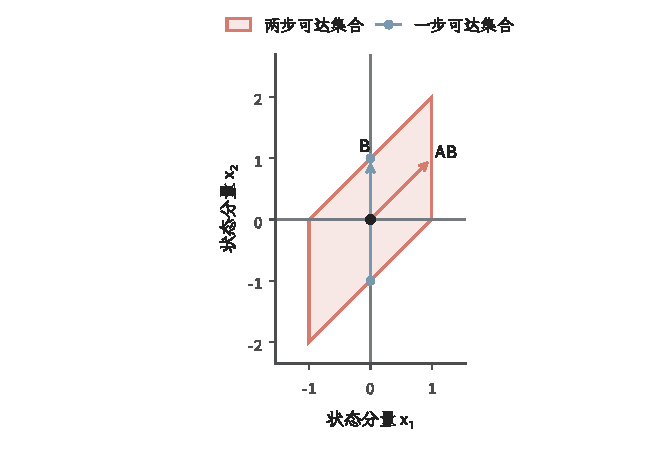
\includegraphics[width=\linewidth]{figures/01-mathematical-preliminaries/05-dynamical-systems-control-decision-and-games/matplotlib/concepts-dynamics/reachable-directions.pdf}
  \caption{教学系统$\bm A=\left[\begin{smallmatrix}1&1\\0&1\end{smallmatrix}\right]$、
  $\bm B=(0,1)^\top$从零出发。蓝色线段为$|u_0|\leq1$的一步可达集合，
  红色区域为$|u_0|,|u_1|\leq1$的两步可达集合；箭头为$\bm B$与$\bm A\bm B$。
  幅值限制用于显示可达区域，不属于无约束可控性秩判据的假设。}
  \label{fig:control-reachable-directions}
\end{figure}

连续时间系统$\dot{\bm x}_t=\bm A\bm x_t+\bm B\bm u_t$在固定$T>0$上的终态为
\[
  \bm x_T=e^{\bm A T}\bm x_0+
  \int_0^T e^{\bm A(T-s)}\bm B\bm u_s\,\mathrm ds.
\]
这里允许$\bm u\in L^2([0,T];\mathbb R^m)$，不加幅值限制。
输入通过积分累积，对应的\term{可控Gram矩阵}（controllability Gramian）为
\begin{equation}
  \bm W_{\mathrm c}(T)=
  \int_0^T e^{\bm A s}\bm B\bm B^\top e^{\bm A^\top s}\,\mathrm ds.
  \label{eq:control-controllability-gramian}
\end{equation}
系统在$[0,T]$可控当且仅当$\bm W_{\mathrm c}(T)\succ\bm0$。
证明先说明奇异矩阵为什么留下不可达方向，再为正定矩阵构造到达任意目标的输入。
为此计算
\[
  \bm q^\top\bm W_{\mathrm c}(T)\bm q
  =\int_0^T\|\bm B^\top e^{\bm A^\top s}\bm q\|_2^2\,\mathrm ds.
\]
若矩阵奇异，某个非零$\bm q$使连续的非负被积函数恒为零，于是该方向与全部受控
终态增量正交。若矩阵正定，对$\bm d=\bm x_{\mathrm f}-e^{\bm A T}\bm x_0$取
\[
  \bm u_s=\bm B^\top e^{\bm A^\top(T-s)}\bm W_{\mathrm c}(T)^{-1}\bm d,
\]
代回便得到终态增量$\bm d$。被积函数恒为零使
$\bm B^\top e^{\bm A^\top s}\bm q$恒为零；
对这个向量函数在$s=0$逐阶求导，得到$\bm q^\top\bm A^k\bm B=0$。
反向由矩阵指数级数成立；再结合Cayley--Hamilton定理，
可知连续系统同样由式~\eqref{eq:control-controllability-matrix}判定。
离散情形的对应Gram矩阵为
$\sum_{j=0}^{N-1}\bm A^j\bm B\bm B^\top(\bm A^\top)^j$。
这些结论依赖线性结构，不能用一点的线性化代替非线性系统的全局可控性。

若只想定位哪个模式不受输入影响，可以直接检查左特征向量。
\begin{theorem}[Popov--Belevitch--Hautus（PBH）可控性判据]
\label{thm:control-pbh-controllability}
矩阵对$(\bm A,\bm B)$可控，当且仅当对每个复特征值$\lambda\in\sigma(\bm A)$，
\begin{equation}
  \operatorname{rank}[\lambda\bm I-\bm A\ \bm B]=n.
  \label{eq:control-pbh-controllability}
\end{equation}
等价地，不存在非零左特征向量$\bm q^\ast$同时满足
$\bm q^\ast\bm A=\lambda\bm q^\ast$和$\bm q^\ast\bm B=\bm0$。
\end{theorem}
\begin{proof}
若存在这样的向量，则
$\bm q^\ast\bm A^k\bm B=\lambda^k\bm q^\ast\bm B=\bm0$对所有$k\geq0$成立，
所以可控性矩阵不可能满行秩。
反之，其列空间$\bm R_{\mathrm{reach}}$若不满维，便是一个真$\bm A$不变子空间。
正交补$\bm R_{\mathrm{reach}}^{\perp}$在$\bm A^\ast$下不变。在复数域上，
这个非零有限维不变子空间包含$\bm A^\ast$的一个特征向量$\bm q$。
它正交于$\bm B$的每一列，因此对应的左特征向量满足
$\bm q^\ast\bm B=\bm0$，PBH矩阵在相应特征值处不满秩。
\end{proof}

终点可控仍不保证任意指定的中间状态都能实现。给定整条参考$\bm r_t$，
离散系统要求每一步$\bm r_{t+1}-\bm A\bm r_t\in\operatorname{col}(\bm B)$，
并且解出的输入位于允许集合；连续系统则要求参考绝对连续且
$\dot{\bm r}_t-\bm A\bm r_t=\bm B\bm u_t^r$几乎处处成立。
终点可达回答“能否到那里”，而实现整条参考轨迹还要回答“能否按这条路走”。

\subsection{观测条件下的状态可区分性}
已知输入对输出的贡献可以计算并扣除。因此，比较同一输入下的两个初态时，
只需考虑自由响应。为简化记号，下式中的$\bm y_t$表示已经扣除已知输入贡献的输出，
于是前$n$次输出满足
\begin{equation}
  \begin{bmatrix}\bm y_0\\\bm y_1\\\vdots\\\bm y_{n-1}\end{bmatrix}
  =
  \underbrace{\begin{bmatrix}
    \bm C\\\bm C\bm A\\\vdots\\\bm C\bm A^{n-1}
  \end{bmatrix}}_{\mathcal O(\bm C,\bm A)}\bm x_0.
  \label{eq:control-observability-matrix}
\end{equation}
\begin{definition}[可观测性]
\label{def:control-observability-detectability}
若同一已知输入下的输出序列能够区分任意两个不同初态，称$(\bm C,\bm A)$
可观测（observable）。对上述线性时不变系统，这等价于
$\mathcal O(\bm C,\bm A)$满列秩。
\end{definition}

满列秩使式~\eqref{eq:control-observability-matrix}对初态至多有一个解。
反之，若秩不足，存在$\bm v\neq\bm0$满足$\mathcal O\bm v=\bm0$，
初态$\bm x_0$与$\bm x_0+\bm v$的前$n$次输出便相同。
Cayley--Hamilton定理使以后所有$\bm C\bm A^k\bm v$也是前$n$项的线性组合，
延长观测仍无法区分两者。这同时证明了定义中的等价关系。
对可控性PBH判据取转置，得到可观测性条件
\begin{equation}
  \operatorname{rank}\begin{bmatrix}\lambda\bm I-\bm A\\\bm C\end{bmatrix}=n
  \quad\text{对每个 }\lambda\in\sigma(\bm A).
  \label{eq:control-pbh-observability}
\end{equation}
连续时间在任意固定正时长、无噪声的完整输出上也有相同秩条件；
等价的观测Gram矩阵是
$\int_0^T e^{\bm A^\top s}\bm C^\top\bm C e^{\bm A s}\,\mathrm ds$。

温度模型的$C=1$使无噪声当前读数就能区分状态。有噪声时，同一个读数可能来自
多个状态，结构可观测性并不提供单次误差上界。
第~\ref{sec:dynamical-state-space-filtering}节建立的预测、滤波和平滑还需初态分布与
噪声规律才能计算估计精度。本章接下来使用较弱的可检测条件，判断哪些看不见的误差
仍能自行衰减，而不要求把所有状态都精确恢复。

\section{策略的轨迹收敛与稳定}
\label{sec:control-closed-loop-stability}

可控性判断输入的结构能力，稳定性判断所选反馈实际产生的长期行为。
第~\ref{sec:dynamical-stability-sensitivity}节已区分平衡点稳定、渐近稳定与指数稳定。
在线性定常系统中，以下“稳定矩阵”统一指离散时间特征值模小于$1$，
或连续时间特征值实部小于$0$；它们都给出齐次系统的指数衰减。
有持续噪声时，所讨论的是齐次初始误差衰减和受迫二阶矩有界，不能称为每条路径趋零。

\subsection{不可控与不可观测模式的稳定条件}
反馈$\bm u=-\bm K\bm x$把状态矩阵改为$\bm A-\bm B\bm K$。
这个矩阵的特征值称为闭环极点（closed-loop poles），它们决定线性齐次响应的衰减或增长。
为了使状态偏差最终消退，只需要通过反馈改变原先不衰减的模式；已经自行
衰减的方向可以保留。这个较弱的要求称为稳定化。
\begin{definition}[可稳定性]
\label{def:control-stabilizability}
若存在$\bm K$使$\bm A-\bm B\bm K$稳定，称矩阵对$(\bm A,\bm B)$
可稳定（stabilizable）。稳定区域按系统采用的离散或连续时间确定。
\end{definition}

从可控性走到固定反馈的存在性，还要用到极点配置定理：对实可控对
$(\bm A_{\mathrm c},\bm B_{\mathrm c})$，任给次数等于其状态维数的实首一多项式，
都存在实增益$\bm K_{\mathrm c}$，使该多项式成为
$\bm A_{\mathrm c}-\bm B_{\mathrm c}\bm K_{\mathrm c}$的特征多项式。
因此可以选择全部根位于单位圆内，或在连续时间选择全部根位于左半平面。
这里引用这一标准存在定理；它不是仅由“有限时间可以到达任意终点”一句话直接推出的结论\scite{math-khalil2002nonlinear}

在前面的二维传播例中，取
$\bm A=\left[\begin{smallmatrix}1&1\\0&1\end{smallmatrix}\right]$、
$\bm B=(0,1)^\top$和$\bm K=(k_1,k_2)$，可直接算得
\[
 \det(\lambda\bm I-\bm A+\bm B\bm K)
 =\lambda^2+(k_2-2)\lambda+1-k_2+k_1.
\]
希望闭环根为$0.2,0.5$时，将系数与
$(\lambda-0.2)(\lambda-0.5)=\lambda^2-0.7\lambda+0.1$比较，
得到$k_2=1.3,k_1=0.4$。这个例子展示怎样用固定增益安排谱，而不再逐时刻另选输入序列。

令$\bm R_{\mathrm{reach}}$为可控性矩阵的列空间，选取以其一组基为前若干列的可逆矩阵$\bm T$。
由于$\bm A\bm R_{\mathrm{reach}}\subseteq\bm R_{\mathrm{reach}}$且
$\operatorname{col}(\bm B)\subseteq\bm R_{\mathrm{reach}}$，坐标$\bm z_t=\bm T^{-1}\bm x_t$给出
\[
  \bm T^{-1}\bm A\bm T=
  \begin{bmatrix}\bm A_{\mathrm c}&\bm A_{1,2}\\
                  \bm0&\bm A_{\mathrm{uc}}\end{bmatrix},
  \qquad
  \bm T^{-1}\bm B=\begin{bmatrix}\bm B_{\mathrm c}\\\bm0\end{bmatrix},
\]
其中$(\bm A_{\mathrm c},\bm B_{\mathrm c})$可控。这是可控分解：上块接收输入，
下块只能自行演化。把$\bm K\bm T$写成$[\bm K_{\mathrm c}\ \bm K_{\mathrm{uc}}]$，
闭环矩阵成为
\[
  \begin{bmatrix}
    \bm A_{\mathrm c}-\bm B_{\mathrm c}\bm K_{\mathrm c}
      &\bm A_{1,2}-\bm B_{\mathrm c}\bm K_{\mathrm{uc}}\\
    \bm0&\bm A_{\mathrm{uc}}
  \end{bmatrix}.
\]
可控块可以用极点配置选择稳定特征值，不可控块的特征值却不受反馈影响。
因此可稳定当且仅当不可控块本身稳定，PBH形式为
\begin{equation}
  \operatorname{rank}[\lambda\bm I-\bm A\ \bm B]=n
  \quad\text{对每个 }|\lambda|\geq1.
  \label{eq:control-pbh-stabilizability}
\end{equation}
只需检查$\bm A$的特征值，其余$\lambda$自动满足秩条件；
连续时间把$|\lambda|\geq1$换成$\operatorname{Re}\lambda\geq0$。

\begin{example}[不可控但可稳定的系统]
\label{ex:control-stabilizable-not-controllable}
取
\[
  \bm A=\begin{bmatrix}1.2&0\\0&0.5\end{bmatrix},
  \qquad \bm B=\begin{bmatrix}1\\0\end{bmatrix}.
\]
可控性矩阵$[\bm B\ \bm A\bm B]
=\left[\begin{smallmatrix}1&1.2\\0&0\end{smallmatrix}\right]$仅有秩$1$。
第二个模式不可控，但其特征值$0.5$已经稳定。取$\bm K=(1,0)$，
闭环特征值为$0.2,0.5$，所以系统可稳定。若交换$\bm B$的两个分量，
输入只能作用到$0.5$模式，$1.2$模式不可控，系统便不可稳定。
\end{example}

传感器一侧有对应的问题：无法识别的初始误差，能否不经校正就逐渐消失？
\begin{definition}[可检测性]
\label{def:control-detectability}
若存在$\bm L$使$\bm A-\bm L\bm C$稳定，称$(\bm C,\bm A)$
可检测（detectable）。
\end{definition}
它不要求每个初态都可恢复，只要求不可观测的模式自行稳定。其离散PBH条件为
\begin{equation}
  \operatorname{rank}
  \begin{bmatrix}\lambda\bm I-\bm A\\\bm C\end{bmatrix}=n
  \quad\text{对每个 }|\lambda|\geq1.
  \label{eq:control-pbh-detectability}
\end{equation}
这一等价关系来自转置对偶：$(\bm A^\top,\bm C^\top)$的可控性矩阵的转置，
正是$(\bm C,\bm A)$的观测矩阵。对前者作可控分解，其不可控块对应原系统的
不可观测模式，又有
$\bm A^\top-\bm C^\top\bm L^\top=(\bm A-\bm L\bm C)^\top$。
因此，不可观测块稳定时可配置其余误差模式；存在不可观测的非衰减模式时，
任何$\bm L$都无法移动它。连续时间同样用闭右半平面替换单位圆外。

继续取示例~\ref{ex:control-stabilizable-not-controllable}的$\bm A$。
$\bm C=(1,0)$看得见$1.2$模式，看不见会自行衰减的$0.5$模式，所以不可观测却可检测。
改用$\bm C=(0,1)$便看不到危险模式，任何估计器的确定性初始误差都不能依靠输出
把该方向统一消除。表~\ref{tab:control-structural-properties}汇总四种条件；
输入或观测能否影响全部方向，与是否足以保证长期稳定，是不同的要求。
\begin{table*}[htbp]
  \centering
  \begin{tabularx}{\linewidth}{lXXX}
    \toprule
    性质 & 所比较的对象 & 哪些方向必须处理 & 二维例的判断\\
    \midrule
    可控 & 输入与终态 & 全部状态方向 & 否，输入无法改变第二坐标\\
    可稳定 & 反馈与闭环谱 & 不稳定及临界模式 & 是，$1.2$模式受控\\
    可观测 & 初态与输出序列 & 全部状态方向 & 否，输出不含第二坐标\\
    可检测 & 观测器与误差谱 & 不稳定及临界模式 & 是，$1.2$模式可见\\
    \bottomrule
  \end{tabularx}
  \caption{固定$\bm A=\operatorname{diag}(1.2,0.5)$、
  $\bm B=(1,0)^\top$、$\bm C=(1,0)$比较四种结构条件。
  第二模式虽不可控、不可观测，却自行衰减；若把其特征值改为$1.1$，
  可稳定与可检测也会失败。连续时间按实部判断危险模式。}
  \label{tab:control-structural-properties}
  \label{tab:control-structural-comparison}
\end{table*}

\subsection{状态反馈下的闭环稳定}
\label{sec:control-state-feedback-stability}
结构条件允许稳定化以后，仍需选定反馈并检查实际闭环。线性状态反馈给出
\begin{equation}
  \bm u_t=-\bm K\bm x_t,
  \qquad \bm x_{t+1}=(\bm A-\bm B\bm K)\bm x_t.
  \label{eq:control-state-feedback}
\end{equation}
负号只是增益约定。按定理~\ref{thm:dynamical-discrete-spectral-stability}，
闭环渐近稳定当且仅当$\rho(\bm A-\bm B\bm K)<1$。
也可以按定理~\ref{thm:dynamical-discrete-lyapunov-equation}找$\bm P\succ\bm0$，
使$\bm P-\bm F^\top\bm P\bm F\succ\bm0$，其中$\bm F=\bm A-\bm B\bm K$。
连续时间则检查$\bm F$的特征值实部或
$\bm F^\top\bm P+\bm P\bm F\prec\bm0$。

不同稳定增益并不产生同样的响应。在无约束、无噪声的温度模型中先以零为目标，
取$u_t=-kx_t$，有$x_t=(0.8-k)^t x_0$。增益$k=0.3$使系数为$0.5$，
$k=0.7$使系数为$0.1$；对相同初态，后者每步收缩更多，却把初始输入幅值
从$0.3|x_0|$提高到$0.7|x_0|$。取$k=1.4$则得到$-0.6$，
状态交替过零，收敛反而比$0.5$慢。稳定范围是$-0.2<k<1.8$，
不是增益越大越快；有饱和时这些线性计算也不再直接适用。

多维系统还要区分渐近速度与瞬态放大。比较
\[
  \bm F_1=0.5\bm I,\qquad
  \bm F_2=\begin{bmatrix}0.5&4\\0&0.5\end{bmatrix}.
\]
二者特征值均为$0.5$，但从$(0,1)^\top$出发，第一步的状态范数分别为
$0.5$和$\sqrt{16.25}>4$。事实上
\[
  \bm F_2^t=
  \begin{bmatrix}0.5^t&4t\,0.5^{t-1}\\0&0.5^t\end{bmatrix}
  \quad(t\geq1).
\]
非对角耦合先放大误差，随后才被指数衰减压低。两者都可以在$\bm A=\bm B=\bm I$
的系统中由$\bm K_i=\bm I-\bm F_i$实现，第二种增益也引入较强的交叉输入。
因此评价反馈时应共同看$\|\bm F^t\|_2$、输入$\|\bm K\bm x_t\|_2$与长期衰减，
而不是仅比较最大特征值。二次成本在下一小节把状态偏差与输入幅值纳入同一准则，
但“稳定”本身并没有选定这一偏好。

非线性系统无法靠一个常矩阵描述全部区域。此时可以先找一个衡量偏离程度的函数，
再选动作让它下降，这就是控制Lyapunov方法。
\begin{definition}[控制Lyapunov函数条件]
\label{def:control-clf}
考虑$\dot{\bm x}_t=\bm f(\bm x_t)+\bm G(\bm x_t)\bm u_t$，目标为原点，
输入属于$U$。若某邻域内的$C^1$函数$V$满足$V(\bm0)=0$、
$V(\bm x)>0$（$\bm x\neq\bm0$），且有正定连续函数$W$使
\[
  \inf_{\bm u\in U}
  \nabla V(\bm x)^\top(\bm f(\bm x)+\bm G(\bm x)\bm u)
  \leq-W(\bm x),
\]
称$V$提供一个\term{控制Lyapunov函数}（control Lyapunov function, CLF）条件：
每个非零状态至少应能选择一个使偏离量严格下降的动作。
调用反馈稳定性结论时，还要求下降动作确实可取到。
\end{definition}

点态存在动作不等于已经构造出适定反馈。若能选出局部Lipschitz反馈$\kappa$，
使原点为平衡、且沿闭环$\dot V\leq-W$，即可回用
定理~\ref{thm:dynamical-nonlinear-lyapunov}得到局部渐近稳定。
若进一步有$c_1\|\bm x\|_2^2\leq V\leq c_2\|\bm x\|_2^2$和
$W\geq c_3\|\bm x\|_2^2$，便有
$V_t\leq e^{-c_3t/c_2}V_0$；全局结论还需全域条件与解的延拓。
例如$\dot x_t=x_t^3+u_t$取$V(x)=x^2/2$、$u_t=-x_t^3-kx_t$（$k>0$），
得到$\dot V=-kx_t^2$和$x_t=e^{-kt}x_0$。这个反馈在无界输入下成立；
若$|u_t|\leq u_{\max}$，大状态处抵消$x_t^3$所需的动作可能不可行，
只能在经过核验的区域中声明稳定\scite{math-khalil2002nonlinear}

\subsection{二次反馈下的稳定化解}
\label{sec:control-lqr-riccati}
要在减小状态偏差与限制输入幅值之间作出具体选择，可以分别给两者加上二次代价。
这一特例能够通过逐步配方直接算出反馈，无须先掌握一般价值优化理论。
\begin{definition}[有限时域线性二次调节]
\label{def:control-finite-horizon-lqr}
考虑状态完全可见的系统
\begin{equation}
  \bm x_{t+1}=\bm A\bm x_t+\bm B\bm u_t+\bm w_{t+1},
  \qquad t=0,\ldots,T-1,
  \label{eq:control-lqr-dynamics}
\end{equation}
以及风险中性的期望成本
\begin{equation}
  J=\mathbb E\left[
  \bm x_T^\top\bm Q_T\bm x_T+
  \sum_{t=0}^{T-1}
  (\bm x_t^\top\bm Q\bm x_t+\bm u_t^\top\bm R\bm u_t)\right].
  \label{eq:control-lqr-cost}
\end{equation}
其中$\bm Q,\bm Q_T\succeq\bm0$为$n\times n$对称矩阵，
$\bm R\succ\bm0$为$m\times m$对称矩阵。输入无幅值限制。
在非预见的状态反馈策略中最小化$J$，称为\term{线性二次调节}
（linear-quadratic regulation, LQR）。
\end{definition}

本小节的$\bm w_t$服从固定但不必高斯的分布，均值为零，协方差为
$\bm\Sigma_{\mathrm w}$，各时刻独立并独立于初态；初态二阶矩有限。
动作对截至$t$的状态历史$\mathcal F_t=\sigma(\bm x_0,\ldots,\bm x_t)$可测，
因而$\bm w_{t+1}$独立于当前状态和动作。状态代价半正定允许某些方向不直接计价，
控制代价正定保证每一步动作最小化严格凸。

用$\Pi_t$表示从$t$到$T-1$、适应上述状态信息的允许策略，
以$\mathbb E_{t,\bm x}$表示从时刻$t$的状态$\bm x$开始运行所得的期望。
最优剩余成本定义为
\[
  \begin{aligned}
  V_t(\bm x)=\inf_{\pi\in\Pi_t}\mathbb E_{t,\bm x}\biggl[
    &\bm x_T^\top\bm Q_T\bm x_T\\
    &+\sum_{\tau=t}^{T-1}
      (\bm x_\tau^\top\bm Q\bm x_\tau+
       \bm u_\tau^\top\bm R\bm u_\tau)\biggr].
  \end{aligned}
\]
这里的下确界取遍反馈策略而不是预先固定的动作序列；
终端为$V_T(\bm x)=\bm x^\top\bm Q_T\bm x$。
将当前阶段与未来分开，条件期望的迭代性质给出
\begin{equation}
  \begin{aligned}
  V_t(\bm x)=\min_{\bm u}\bigl\{&
    \bm x^\top\bm Q\bm x+\bm u^\top\bm R\bm u\\
    &+\mathbb E[V_{t+1}(\bm A\bm x+\bm B\bm u+\bm w_{t+1})]\bigr\}.
  \end{aligned}
  \label{eq:control-lqr-bellman}
\end{equation}
对任意策略，后续成本至少为下一状态的$V_{t+1}$；若下一步的下界可由反馈取得，
先选当前极小动作，再接上该反馈，就取得等号。下面的反向归纳同时构造这些可取到的
动作，因此这里不依赖尚未证明的一般最优策略存在性。这一递推的通用形式将在
第~\ref{chap:decision-theory-and-dynamic-risk}章展开\scite{math-anderson2007lqr}

\begin{theorem}[有限时域LQR与Riccati递推]
\label{thm:control-finite-horizon-lqr}
在上述条件下，
$V_t(\bm x)=\bm x^\top\bm P_t\bm x+c_t$，
其中$\bm P_T=\bm Q_T$、$c_T=0$。令
\begin{equation}
  \begin{aligned}
    \bm S_t&=\bm R+\bm B^\top\bm P_{t+1}\bm B,\\
    \bm K_t&=\bm S_t^{-1}\bm B^\top\bm P_{t+1}\bm A,
  \end{aligned}
  \label{eq:control-lqr-gain}
\end{equation}
则最优动作是$\bm u_t^\ast=-\bm K_t\bm x_t$，矩阵满足
\begin{equation}
  \begin{aligned}
  \bm P_t={}&\bm Q+\bm A^\top\bm P_{t+1}\bm A\\
       &-\bm A^\top\bm P_{t+1}\bm B\bm S_t^{-1}
                    \bm B^\top\bm P_{t+1}\bm A,
  \end{aligned}
  \label{eq:control-discrete-riccati-recursion}
\end{equation}
噪声只进入常数项
\begin{equation}
  c_t=c_{t+1}+\operatorname{tr}(\bm P_{t+1}\bm\Sigma_{\mathrm w}).
  \label{eq:control-lqr-noise-constant}
\end{equation}
\end{theorem}
\begin{proof}
在终端结论成立。假设$t+1$时刻的表达和最优反馈已构造，
记$\bm z=\bm A\bm x+\bm B\bm u$。噪声的零均值、协方差与独立性给出
\[
  \mathbb E[V_{t+1}(\bm z+\bm w_{t+1})]
  =\bm z^\top\bm P_{t+1}\bm z+
    \operatorname{tr}(\bm P_{t+1}\bm\Sigma_{\mathrm w})+c_{t+1}.
\]
交叉项条件期望为零。将$\bm z$展开，当前目标为
\begin{align*}
  &\bm x^\top(\bm Q+\bm A^\top\bm P_{t+1}\bm A)\bm x
   +2\bm u^\top\bm B^\top\bm P_{t+1}\bm A\bm x
   +\bm u^\top\bm S_t\bm u\\
  &\qquad+\operatorname{tr}(\bm P_{t+1}\bm\Sigma_{\mathrm w})+c_{t+1}.
\end{align*}
由$\bm P_{t+1}\succeq\bm0$、$\bm R\succ\bm0$得$\bm S_t\succ\bm0$。
动作相关项可以完整配方：
\begin{align*}
  &\bm u^\top\bm S_t\bm u+
       2\bm u^\top\bm B^\top\bm P_{t+1}\bm A\bm x\\
  &\quad=(\bm u+\bm K_t\bm x)^\top\bm S_t(\bm u+\bm K_t\bm x)
       -\bm x^\top\bm K_t^\top\bm S_t\bm K_t\bm x.
\end{align*}
平方项非负且仅在$\bm u=-\bm K_t\bm x$处为零。合并剩余二次项与常数项，
分别得到式~\eqref{eq:control-discrete-riccati-recursion}和
式~\eqref{eq:control-lqr-noise-constant}。所得二次型也是
\[
  \bm x^\top\bm P_t\bm x
  =\min_{\bm u}\{
   \bm x^\top\bm Q\bm x+\bm u^\top\bm R\bm u+
   (\bm A\bm x+\bm B\bm u)^\top\bm P_{t+1}(\bm A\bm x+\bm B\bm u)\},
\]
故$\bm P_t\succeq\bm0$，归纳可以继续。线性极小动作可测，并在有限时域保持二阶矩
有限；将这些动作依次拼接，取得每一步下界，证明最优值确实可达。
\end{proof}

线性动态把二次型变为状态与动作的联合二次型，动作配方后又留下状态二次型。
这解释了Riccati构造为何在本模型中闭合，也说明不能把非线性动态随意换成Jacobian
就声称得到了原问题的精确解。
噪声只影响常数项同样有边界：非零均值通常产生线性项和仿射偏置；
噪声分布随动作或状态变化时，增益也可能变化；若目标更加重视成本很大的
少数结果，即后文的尾部风险，原增益同样未必最优。
若权重和噪声协方差是预先给定的逐时量，只需在第$t$步分别用
$\bm Q_t,\bm R_t,\bm\Sigma_{\mathrm w,t+1}$替换对应矩阵，
保持$\bm Q_t\succeq\bm0,\bm R_t\succ\bm0$和独立零均值条件，同一反向归纳仍成立。

为了看清有限时域的成本最优为何未必保证长期稳定，下面把温度模型的衰减系数
$0.8$改为增长系数$1.2$，考察无输入时会放大状态的标量系统。
取$x_{t+1}=1.2x_t+u_t$、$Q=R=1$且无噪声。记下一步系数为$p=P_{t+1}$，
当前目标的配方为
\[
  \begin{aligned}
  x^2+u^2+p(1.2x+u)^2
   ={}&(1+p)\left(u+\frac{1.2p}{1+p}x\right)^2\\
     &+\left(1+1.44p-\frac{1.44p^2}{1+p}\right)x^2.
  \end{aligned}
\]
因此
\[
  S_t=1+P_{t+1},\qquad
  K_t=\frac{1.2P_{t+1}}{1+P_{t+1}},
  \qquad
  P_t=1+\frac{1.44P_{t+1}}{1+P_{t+1}}.
\]
若$P_T=0$，则$P_{T-1}=1,K_{T-1}=0$；
最后一个动作之后没有状态代价，故此时不用力。
再向前一步有$P_{T-2}=1.72,K_{T-2}=0.6$。
有限时域的最优反馈未必在每一步都使闭环矩阵稳定，$K_{T-1}=0$就是反例。
所以有限时域内能够通过配方求出最优动作，并不能证明无限时域内存在稳定的
最优反馈。

为处理长期稳定化，现切换到确定性、时不变、无折扣系统，即
$\bm w_{t+1}=\bm0$，目标为
\[
  J_\infty=\sum_{t=0}^\infty
  (\bm x_t^\top\bm Q\bm x_t+\bm u_t^\top\bm R\bm u_t).
\]
若反馈与二次系数不再随时间变化，递推给出
\term{离散代数Riccati方程}（discrete algebraic Riccati equation, DARE）：
\begin{equation}
  \begin{aligned}
  \bm P={}&\bm Q+\bm A^\top\bm P\bm A\\
     &-\bm A^\top\bm P\bm B
       (\bm R+\bm B^\top\bm P\bm B)^{-1}\bm B^\top\bm P\bm A.
  \end{aligned}
  \label{eq:control-dare}
\end{equation}
所需的\term{稳定化解}（stabilizing solution）不仅满足$\bm P\succeq\bm0$，
还要求其增益
$\bm K=(\bm R+\bm B^\top\bm P\bm B)^{-1}\bm B^\top\bm P\bm A$
使闭环稳定。

\begin{theorem}[无限时域LQR的稳定化解]
\label{thm:control-infinite-horizon-lqr}
设$\bm Q\succeq\bm0$、$\bm R\succ\bm0$，
$(\bm A,\bm B)$可稳定且$(\bm Q^{1/2},\bm A)$可检测。
则式~\eqref{eq:control-dare}存在唯一半正定稳定化解$\bm P$。
相应反馈使闭环渐近稳定，并在所有允许控制序列中给出无折扣二次总成本的
最优值$V(\bm x)=\bm x^\top\bm P\bm x$。
\end{theorem}
\begin{proof}
取长度$N$、终端代价为零的有限问题，记其初始价值矩阵为$\bm P^{(N)}$。
增加一个非负阶段成本不能降低最优成本，故
$\bm0\preceq\bm P^{(N)}\preceq\bm P^{(N+1)}$。
可稳定性提供$\overline{\bm K}$使
$\overline{\bm F}=\bm A-\bm B\overline{\bm K}$稳定。始终用此反馈的成本矩阵为
\[
  \overline{\bm P}=\sum_{j=0}^\infty
  (\overline{\bm F}^\top)^j
  (\bm Q+\overline{\bm K}^\top\bm R\overline{\bm K})
  \overline{\bm F}^j,
\]
级数由指数衰减收敛，且$\bm P^{(N)}\preceq\overline{\bm P}$。
每个二次型$\bm x^\top\bm P^{(N)}\bm x$单调有界，
再用极化恒等式恢复矩阵各元素，得到$\bm P^{(N)}\to\bm P\succeq\bm0$。
Riccati映射连续，因为待逆矩阵始终不小于$\bm R\succ\bm0$；
对$\bm P^{(N+1)}=\mathcal R(\bm P^{(N)})$取极限得到DARE。

令$\bm F=\bm A-\bm B\bm K$，DARE按增益改写为
\begin{equation}
  \bm P-\bm F^\top\bm P\bm F=\bm Q+\bm K^\top\bm R\bm K.
  \label{eq:control-dare-lyapunov}
\end{equation}
若$\bm F\bm z=\lambda\bm z$且$\bm z\neq\bm0,|\lambda|\geq1$，
在两侧乘$\bm z^\ast,\bm z$得到
\[
  (1-|\lambda|^2)\bm z^\ast\bm P\bm z
  =\|\bm Q^{1/2}\bm z\|_2^2+\|\bm R^{1/2}\bm K\bm z\|_2^2.
\]
左侧非正，右侧非负，所以均为零，特别有
$\bm Q^{1/2}\bm z=\bm0,\bm K\bm z=\bm0$。
于是$\bm A\bm z=(\bm F+\bm B\bm K)\bm z=\lambda\bm z$，
违反$(\bm Q^{1/2},\bm A)$的可检测性。因此$\bm F$稳定。

存在且稳定还不足以完成最优性证明。记$\bm S=\bm R+\bm B^\top\bm P\bm B$，
对任意控制沿前$N$步累加配方恒等式：
\begin{align*}
  &\sum_{t=0}^{N-1}
    (\bm x_t^\top\bm Q\bm x_t+\bm u_t^\top\bm R\bm u_t)
    +\bm x_N^\top\bm P\bm x_N\\
  &\quad=\bm x_0^\top\bm P\bm x_0+
    \sum_{t=0}^{N-1}
    (\bm u_t+\bm K\bm x_t)^\top\bm S(\bm u_t+\bm K\bm x_t).
\end{align*}
不能直接丢弃左侧终端项。若该控制的总成本有限，非负级数的项趋零，给出
$\bm Q^{1/2}\bm x_t\to\bm0$及$\bm u_t\to\bm0$，后者使用$\bm R\succ\bm0$。
可检测性提供$\bm L$使$\bm H=\bm A-\bm L\bm Q^{1/2}$稳定，于是
\[
  \bm x_{t+1}=\bm H\bm x_t+
       \underbrace{\bm B\bm u_t+\bm L\bm Q^{1/2}\bm x_t}_{\bm d_t\to\bm0}.
\]
展开为$\bm H^t\bm x_0+\sum_{j=0}^{t-1}\bm H^{t-1-j}\bm d_j$。
有限个早期输入的贡献随$t$衰减；晚期输入任意小，且
$\sum_{j\geq0}\|\bm H^j\|_2<\infty$，故卷积尾部也趋零。
因此$\bm x_t\to\bm0$，终端项趋零。

令$N\to\infty$，任何有限成本控制的成本都是
$\bm x_0^\top\bm P\bm x_0$加上一串非负平方项。
采用$\bm u_t=-\bm K\bm x_t$时平方项全为零，闭环稳定保证终端项趋零和总成本有限，
故达到下界；无限成本控制自然不能优于它。
若另有半正定稳定化解，同一配方和终端项论证也使它表示全部初态上的同一个最优成本。
两个对称矩阵的二次型处处相等，矩阵便相等，唯一性得证。
\end{proof}

在前述$A=1.2,B=1,Q=R=1$例中，
\[
  P=1+\frac{1.44P}{1+P},
  \qquad P^2-1.44P-1=0,
\]
半正定根与反馈为
\[
  P=\frac{1.44+\sqrt{6.0736}}2\approx1.952,
  \quad K=\frac{1.2P}{1+P}\approx0.794,
  \quad 1.2-K\approx0.406.
\]
另一个根为负，不表示非负总成本。
可检测条件中的“输出”是成本所见的$\bm Q^{1/2}\bm x$，不是传感器的$\bm C\bm x$；
两种可检测条件不能替换。

若$A=1.2,B=1,Q=0,R=1$，系统可控却不满足成本可检测性。
DARE有$P=0$与$P=0.44$两个半正定根。前者给$K=0$和不稳定闭环$1.2$，
后者给稳定闭环$5/6$。原目标只惩罚控制，$u_t=0$以零成本全局最优，
稳定化反馈反而支付正成本。这个反例说明稳定化与成本最优之间的联系确实依赖假设。
若恢复持续非零加性噪声，稳定闭环通常有非零稳态协方差，单步期望成本不趋零，
无折扣总期望成本通常发散；除噪声传播恰好不被成本计价等退化情形，
应改用有限、折扣或长期平均成本，而不是沿用本定理的确定性总成本。

连续时间也可以直接用代数方程构造稳定反馈，无须先推导有限时域价值。
对$\dot{\bm x}_t=\bm A\bm x_t+\bm B\bm u_t$，连续代数Riccati方程
（continuous algebraic Riccati equation, CARE）为
\begin{equation}
  \bm0=\bm Q+\bm A^\top\bm P+\bm P\bm A
       -\bm P\bm B\bm R^{-1}\bm B^\top\bm P.
  \label{eq:control-care}
\end{equation}
当$\bm Q\succeq\bm0,\bm R\succ\bm0$，且连续时间意义下
$(\bm A,\bm B)$可稳定、$(\bm Q^{1/2},\bm A)$可检测时，CARE有唯一半正定
稳定化解；这是连续线性二次控制的标准代数结论\scite{math-anderson2007lqr}
本处使用其存在性，具体闭环性质还可直接核验。
令$\bm K=\bm R^{-1}\bm B^\top\bm P$、$\bm F=\bm A-\bm B\bm K$，则
\[
  \bm F^\top\bm P+\bm P\bm F=-(\bm Q+\bm K^\top\bm R\bm K).
\]
若$\bm F\bm z=\lambda\bm z$且$\operatorname{Re}\lambda\geq0$，
两侧二次型给出
$2\operatorname{Re}\lambda\,\bm z^\ast\bm P\bm z
=-\|\bm Q^{1/2}\bm z\|_2^2-\|\bm R^{1/2}\bm K\bm z\|_2^2$。
同样推出$\bm Q^{1/2}\bm z=\bm K\bm z=\bm0$，与可检测性矛盾。
所以闭环谱位于左半平面；即使$\bm P$仅半正定，仍可由谱结论另解正定Lyapunov方程。
连续有限时域微分Riccati及价值最优性在
第~\ref{chap:decision-theory-and-dynamic-risk}章主讲；本处的稳定核验不以它们为前提。

\subsection{输出反馈下的估计与闭环稳定}
\label{sec:control-output-feedback-stability}
前面的反馈把真实状态直接写入动作公式。若控制器只有传感器读数，就需要说明
怎样结合模型与读数形成状态估计，以及使用哪一时刻的估计计算动作。
\term{Luenberger观测器}（Luenberger observer）采用
\begin{equation}
  \widehat{\bm x}_{t+1}
  =\bm A\widehat{\bm x}_t+\bm B\bm u_t+
    \bm L(\bm y_t-\bm C\widehat{\bm x}_t).
  \label{eq:control-luenberger-observer}
\end{equation}
无噪声时，误差$\bm e_t^{\mathrm o}=\bm x_t-\widehat{\bm x}_t$满足
$\bm e_{t+1}^{\mathrm o}=(\bm A-\bm L\bm C)\bm e_t^{\mathrm o}$。
可检测性恰好允许选出误差衰减的$\bm L$。
若使用$\bm u_t=-\bm K\widehat{\bm x}_t$，联合系统为
\begin{equation}
  \begin{bmatrix}\bm x_{t+1}\\\bm e_{t+1}^{\mathrm o}\end{bmatrix}
  =
  \begin{bmatrix}
    \bm A-\bm B\bm K&\bm B\bm K\\
    \bm0&\bm A-\bm L\bm C
  \end{bmatrix}
  \begin{bmatrix}\bm x_t\\\bm e_t^{\mathrm o}\end{bmatrix}.
  \label{eq:control-separation-block}
\end{equation}
这个\term{分离原理}（separation principle）说的是闭环谱可以分开设计：
特征行列式等于两个对角块特征行列式之积，故联合谱恰为二者的并集。
当两块都稳定时，联合矩阵稳定；反过来，任一块的危险特征值也保留在联合谱中。
因而确定性观测器与状态反馈可以分别作稳定设计；这一论证并未涉及成本最优。

有噪声时，还需区分预测协方差与观测更新后的协方差。
在式~\eqref{eq:control-lqr-dynamics}及
$\bm y_t=\bm C\bm x_t+\bm v_t$中，令$\bm w_t,\bm v_t$分别为独立同分布零均值
噪声，协方差为$\bm\Sigma_{\mathrm w}\succeq\bm0,\bm\Sigma_{\mathrm v}\succ\bm0$，
两族与初态相互独立，初态二阶矩有限，估计器从先验均值及协方差初始化。
若要将Kalman估计解释为精确条件均值，再要求初态和噪声联合高斯；
非高斯时以下递推仍描述相应线性滤波器的误差矩，不自动描述完整后验。

以$\bm\Pi_t$记看到$\bm y_t$之前的预测误差协方差。高斯情形下，
$\widehat{\bm x}_{t|t-1}$是给定截至$t-1$的观测及已执行控制后的条件均值。
在初始时刻，$\bm\Pi_0$由尚未使用$y_0$的先验给出。
更新增益$\bm M_t$与合并预测增益$\bm L_t$分别为
\[
  \bm M_t=\bm\Pi_t\bm C^\top
       (\bm C\bm\Pi_t\bm C^\top+\bm\Sigma_{\mathrm v})^{-1},
  \qquad \bm L_t=\bm A\bm M_t.
\]
先更新再预测，可以写成
\[
  \widehat{\bm x}_{t+1|t}
  =\bm A\widehat{\bm x}_{t|t-1}+\bm B\bm u_t+
       \bm L_t(\bm y_t-\bm C\widehat{\bm x}_{t|t-1}).
\]
所以预测误差的齐次矩阵为$\bm A-\bm L_t\bm C$，不能遗漏增益中的$\bm A$。
稳态预测协方差满足
\begin{equation}
  \begin{aligned}
  \bm\Pi={}&\bm A\bm\Pi\bm A^\top+\bm\Sigma_{\mathrm w}\\
     &-\bm A\bm\Pi\bm C^\top
       (\bm C\bm\Pi\bm C^\top+\bm\Sigma_{\mathrm v})^{-1}
       \bm C\bm\Pi\bm A^\top.
  \end{aligned}
  \label{eq:control-filter-dare}
\end{equation}
控制DARE中作$\bm A\mapsto\bm A^\top,\bm B\mapsto\bm C^\top,
\bm Q\mapsto\bm\Sigma_{\mathrm w},\bm R\mapsto\bm\Sigma_{\mathrm v}$便得到此式。
公式的转置对偶联系的是两个矩阵计算问题，并不使状态成本与估计协方差具有相同含义。

\begin{theorem}[稳态预测滤波的充分条件]
\label{thm:control-steady-filter}
若$(\bm C,\bm A)$可检测、$(\bm A,\bm\Sigma_{\mathrm w}^{1/2})$可稳定，
且$\bm\Sigma_{\mathrm v}\succ\bm0$，则式~\eqref{eq:control-filter-dare}
有唯一半正定稳定化解$\bm\Pi$。从任意有限$\bm\Pi_0\succeq\bm0$出发的
预测协方差递推收敛到$\bm\Pi$，稳态$\bm L=\bm A\bm M$使
$\bm A-\bm L\bm C$稳定。
\end{theorem}
\begin{proof}
对偶代换把本定理的两个结构条件分别变为无限LQR定理的可稳定、可检测条件，
故解的存在、唯一与稳定性成立。为说明一般初始协方差的收敛，记滤波Riccati映射为
$\Phi$。固定任意合并增益$\bm L$，定义
\[
  \Psi_{\bm L}(\bm X)
  =(\bm A-\bm L\bm C)\bm X(\bm A-\bm L\bm C)^\top+
     \bm\Sigma_{\mathrm w}+\bm L\bm\Sigma_{\mathrm v}\bm L^\top.
\]
配方表明$\Phi(\bm X)\preceq\Psi_{\bm L}(\bm X)$，等号在对应Kalman增益处成立。
又若$\bm X\succeq\bm Y$，每个固定增益下
$\Psi_{\bm L}(\bm X)\succeq\Psi_{\bm L}(\bm Y)$；
取$\bm X$的极小增益便得$\Phi(\bm X)\succeq\Phi(\bm Y)$。
取稳态增益$\bm L$，有$\Psi_{\bm L}(\bm\Pi)=\bm\Pi$，并由单调性归纳得到
\[
  \Phi^t(\bm0)\preceq\Phi^t(\bm\Pi_0)
                     \preceq\Psi_{\bm L}^t(\bm\Pi_0).
\]
左端按对偶有限时域构造收敛到$\bm\Pi$；
右端与$\bm\Pi$之差为
$(\bm A-\bm L\bm C)^t(\bm\Pi_0-\bm\Pi)
 [(\bm A-\bm L\bm C)^\top]^t$，也趋零，夹逼得证。
\end{proof}

稳态滤波误差仍由新噪声持续驱动：
\[
  \bm e_{t+1}^{\mathrm p}
  =(\bm A-\bm L\bm C)\bm e_t^{\mathrm p}
     +\bm w_{t+1}-\bm L\bm v_t.
\]
稳定性使初始误差的影响衰减，协方差趋于有限的$\bm\Pi$，
并不使噪声消失。温度例取$\Sigma_{\mathrm w}=0.04,\Sigma_{\mathrm v}=0.09$，
稳态方程为
$\Pi=0.64\Pi+0.04-0.64\Pi^2/(\Pi+0.09)$，
即$\Pi^2-0.0076\Pi-0.0036=0$。正根约为$0.06392$，
$M\approx0.4153,L\approx0.3322$，预测齐次误差系数约为$0.4678$；
稳态预测误差方差为正：即使初始估计误差已消退，新噪声仍会不断造成偏差，
所以不能说每条估计误差路径都趋于零。

实际控制可使用当前观测更新后的$\widehat{\bm x}_{t|t}$。
取$\bm u_t=-\bm K\widehat{\bm x}_{t|t}$，并用预测误差
$\bm e_t^{\mathrm p}=\bm x_t-\widehat{\bm x}_{t|t-1}$，
齐次联合矩阵变为
\[
  \begin{bmatrix}
    \bm A-\bm B\bm K&\bm B\bm K(\bm I-\bm M\bm C)\\
    \bm0&\bm A(\bm I-\bm M\bm C)
  \end{bmatrix}.
\]
附加噪声为
$((\bm w_{t+1}-\bm B\bm K\bm M\bm v_t)^\top,
  (\bm w_{t+1}-\bm A\bm M\bm v_t)^\top)^\top$，
两分量相关，但联合协方差仍有限。
两个对角块稳定时，联合齐次系统稳定；
用幂级数展开协方差，便得有限初始二阶矩下的二阶矩有界和稳态协方差收敛。
非零持续噪声下，状态与预测误差的均值可以趋零，但每次运行仍会受到新噪声扰动，
其样本路径一般不会趋于零。
有限时域线性二次高斯控制的期望成本最优性由
第~\ref{chap:decision-theory-and-dynamic-risk}章另证。
受控观测、输入约束、非线性或模型错设可能改变信息与误差动态，
不能从这里的谱分离直接推出稳定，更不能直接推出最优。

\section{策略的调节与跟踪}
\label{sec:control-regulation-tracking}

前面的反馈围绕原点设计，但温度通常要维持在非零设定值，机械位置也可能要跟随
持续移动的目标。两类任务都能转化为误差系统的稳定问题，区别在于维持目标所需的
输入是常数还是随时间变化。转化前必须先核对目标本身是否符合系统规律。

\subsection{固定目标下的轨迹调节}
\subsubsection{目标平衡与可行输入}
设定值（setpoint）是希望状态或输出最终保持的常数。\term{调节}（regulation）要求偏离
该常数的误差趋于零；它不只要求在某一时刻经过目标。
\begin{definition}[目标平衡与调节误差]
\label{def:control-regulation-equilibrium}
对$\bm x_{t+1}=\bm A\bm x_t+\bm B\bm u_t$，
状态设定值$\bm r$与常值输入$\bm u^r$构成目标平衡，若
\begin{equation}
  (\bm I-\bm A)\bm r=\bm B\bm u^r.
  \label{eq:control-target-equilibrium}
\end{equation}
状态调节误差定义为$\bm e_t=\bm x_t-\bm r$。
若只指定输出设定值$\bm q$，还需寻找平衡状态$\bm r$使
$\bm C\bm r=\bm q$，输出误差为$\bm e_t^y=\bm C\bm x_t-\bm q$。
有输入、状态限制时，目标平衡还须满足$\bm u^r\in U,\bm r\in S$。
\end{definition}

对只指定输出的任务，可解联立方程
\[
  \begin{bmatrix}\bm I-\bm A&-\bm B\\\bm C&\bm0\end{bmatrix}
  \begin{bmatrix}\bm r\\\bm u^r\end{bmatrix}
  =\begin{bmatrix}\bm0\\\bm q\end{bmatrix}.
\]
方程可能无解或有多个解；输出达到设定值也不自动要求所有内部状态相同。
连续时间的平衡条件相应为$\bm A\bm r+\bm B\bm u^r=\bm0$。
这些平衡方程是任务可行性的检查，不是稳定性证明。

\begin{example}[非零温度需要维持输入]
\label{ex:control-temperature-equilibrium}
在无噪声温度模型中，设定值$r=2$要求
$2=0.8\times2+u^r$，所以$u^r=0.4$。
若直接使用$u_t=-0.3(x_t-2)$，在$x_t=2$处输入变成零，
下一步温差便降为$1.6$，因而$2$不是闭环平衡。
若执行器要求$0\leq u\leq1$，单从平衡输入看，
$u^r=0.2r$允许$0\leq r\leq5$；再加状态限制$0\leq x\leq3$，
则目标必须落在$[0,3]$。$r=2,u^r=0.4$满足这两项必要条件。
从某个初态走到目标期间是否也满足约束，还需检查整段闭环轨迹。
\end{example}

\subsubsection{基于误差反馈的轨迹调节}
平衡输入抵消目标位置的自然漂移，反馈只负责消除偏差。对已求得的平衡对取
\begin{equation}
  \bm u_t=\bm u^r-\bm K(\bm x_t-\bm r),
  \qquad
  \bm e_{t+1}=(\bm A-\bm B\bm K)\bm e_t.
  \label{eq:control-regulation-feedback}
\end{equation}
第二式由原动态减去平衡方程得到。只要闭环矩阵稳定，
$\bm e_t\to\bm0$，便有$\bm x_t\to\bm r$与
$\bm u_t\to\bm u^r$。如果输出目标通过$\bm C\bm r=\bm q$定义，
也有$\bm e_t^y=\bm C\bm e_t\to\bm0$。

温度反馈的完整计算为
\begin{equation}
  u_t=0.4-0.3(x_t-2),
  \qquad
  e_{t+1}=0.5e_t,\quad e_t=0.5^t(x_0-2).
  \label{eq:control-temperature-regulation}
\end{equation}
从$x_0=0$出发，状态依次为$0,1,1.5,1.75,\ldots$，
输入依次为$1,0.7,0.55,0.475,\ldots$。
状态趋于$2$而输入趋于$0.4$，不是输入也必须趋零。

若改用估计状态$\widehat{\bm x}_t$，令
$\bm e_t^{\mathrm o}=\bm x_t-\widehat{\bm x}_t$，
则调节误差成为
$\bm e_{t+1}=(\bm A-\bm B\bm K)\bm e_t+\bm B\bm K\bm e_t^{\mathrm o}$。
确定性估计误差趋零、调节闭环稳定时，卷积展开仍给出调节误差趋零；
估计噪声持续存在时，只能据噪声条件讨论均值、协方差或误差范围。
对$\bm e_t$与$\bm u_t-\bm u^r$使用LQR也是一种增益选择，
但权重表达的是任务偏好，怎样比较不同累计代价由
第~\ref{chap:decision-theory-and-dynamic-risk}章展开。
达到设定值这一任务本身并未指定哪组权重。

\subsubsection{持续扰动下的轨迹调节}
平衡偏移的计算依赖模型准确。若真实系统含持续加性项$\bm d_t$，
误差满足
\begin{equation}
  \bm e_{t+1}=\bm F\bm e_t+\bm d_t,
  \qquad \bm F=\bm A-\bm B\bm K.
  \label{eq:control-regulation-disturbance}
\end{equation}
这正是第~\ref{sec:dynamical-stability-sensitivity}节的受迫响应：
初始误差按$\bm F^t$衰减，新扰动却在每一步进入。
若$\|\bm F^j\|\leq M\rho^j$、$0<\rho<1$且$\|\bm d_t\|\leq\bar d$，
则
\[
  \|\bm e_t\|\leq M\rho^t\|\bm e_0\|
       +\frac{M(1-\rho^t)}{1-\rho}\bar d.
\]
常值扰动$\bm d$通常留下$\bm e_\infty=(\bm I-\bm F)^{-1}\bm d$，
不能靠初始误差衰减消除。温度例为$e_{t+1}=0.5e_t+d$，
稳态偏差是$2d$。若改为独立高斯$w_{t+1}\sim\mathcal N(0,0.04)$，
均值误差衰减，但
$\operatorname{Var}(e_t)\to0.04/(1-0.5^2)=0.053\overline3$；
二阶矩有界不是样本路径趋于零。

对未知常值偏差，可以让控制器累积过去的误差，并据此继续调整输入。
\term{积分调节}（integral regulation）正是把这段记忆作为额外状态。只要输出误差仍非零，积分状态就会继续变化，
控制器因而不会停留在原来的错误平衡上。对输出误差$\bm C\bm x_t-\bm q=\bm C\bm e_t$取
\begin{equation}
  \begin{aligned}
    \bm z_{t+1}&=\bm z_t+\bm C\bm e_t,\\
    \bm u_t&=\bm u^r-\bm K_x\bm e_t-\bm K_i\bm z_t.
  \end{aligned}
  \label{eq:control-integral-regulation}
\end{equation}
其中$\bm z_t\in\mathbb R^p$为积分状态；采样周期不为$1$时，可将周期因子并入积分增益。
增广误差系统为
\[
  \begin{bmatrix}\bm e_{t+1}\\\bm z_{t+1}\end{bmatrix}
  =
  \underbrace{\begin{bmatrix}
    \bm A-\bm B\bm K_x&-\bm B\bm K_i\\
    \bm C&\bm I
  \end{bmatrix}}_{\bm F_{\mathrm{aug}}}
  \begin{bmatrix}\bm e_t\\\bm z_t\end{bmatrix}
  +\begin{bmatrix}\bm d\\\bm0\end{bmatrix}.
\]
若$\bm F_{\mathrm{aug}}$稳定，则在常值$\bm d$下收敛到唯一平衡；
该平衡的积分方程强制$\bm C\bm e_\infty=\bm0$。
消除的是指定输出的常值误差，不一定是整个状态误差。

积分状态会保留累积误差，自身带有特征值$1$。加入它以后，原反馈稳定也不足以
保证整个系统稳定。因此，设计增益前应检查下面的增广矩阵对是否可稳定：
\[
  \left(
   \begin{bmatrix}\bm A&\bm0\\\bm C&\bm I\end{bmatrix},
   \begin{bmatrix}\bm B\\\bm0\end{bmatrix}\right)
\]
除原系统的危险模式必须可控外，新加入的$\lambda=1$模式要求
\[
  \operatorname{rank}
  \begin{bmatrix}\bm I-\bm A&-\bm B\\\bm C&\bm0\end{bmatrix}=n+p.
\]
这是增广PBH判据在$1$处的展开；对$\lambda\neq1$，积分状态块可消元，
便回到原系统的判据。受约束时还要检查真实扰动下是否存在允许的平衡输入。

\begin{example}[温度系统的积分增广]
\label{ex:control-temperature-integral}
取$e_t=x_t-2$、$z_{t+1}=z_t+e_t$与
$u_t=0.4-0.3e_t-0.1z_t$。常值扰动$d$下，
\[
  \begin{bmatrix}e_{t+1}\\z_{t+1}\end{bmatrix}
  =\begin{bmatrix}0.5&-0.1\\1&1\end{bmatrix}
   \begin{bmatrix}e_t\\z_t\end{bmatrix}
   +\begin{bmatrix}d\\0\end{bmatrix}.
\]
特征多项式为$\lambda^2-1.5\lambda+0.6$，两根
$0.75\pm0.19365\,\mathrm i$的模为$\sqrt{0.6}<1$。
因而$e_t\to0,z_t\to10d,u_t\to0.4-d$。
若$0\leq u\leq1$，平衡输入要求$-0.6\leq d\leq0.4$；
这个条件仍不保证任意初始积分状态的瞬态输入都不饱和。
\end{example}

输入饱和后，真实误差不再服从上述线性增广方程，积分状态却可能继续累积，
造成解除饱和后的大幅动作。限制或回退积分累积是常见的抗积分饱和处理，
但处理后的闭环仍需重新验证。积分器针对常值偏差的消除能力也不能推广为对任意
有界时变扰动的零误差保证。若增广系统稳定，时变有界扰动仍可通过其卷积获得有界误差；
若需保证安全，应进一步按第~\ref{sec:control-safety-cbf}节检查实际输入。

\subsection{运动参考下的轨迹跟踪}
\subsubsection{参考轨迹与可实现条件}
\term{跟踪}（tracking）以随时间变化的状态$\bm r_t$或输出$\bm q_t$为目标，
要求$\bm x_t-\bm r_t$或$\bm C\bm x_t-\bm q_t$趋零或保持在规定范围内。
参考本身可以持续运动，因此不能把跟踪收敛写成状态必须趋于某个固定点。
\begin{definition}[可实现参考]
\label{def:control-realizable-reference}
离散线性系统的参考状态、参考输入为$(\bm r_t,\bm u_t^r)$。
若每一步满足
\begin{equation}
  \bm r_{t+1}=\bm A\bm r_t+\bm B\bm u_t^r,
  \qquad \bm q_t=\bm C\bm r_t,
  \label{eq:control-realizable-reference}
\end{equation}
且参考状态、输入满足所声明的约束，称它为可实现参考。
精确从首时刻跟踪还要求$\bm x_0=\bm r_0$。
连续时间则要求$\bm r_t$绝对连续，并有
$\dot{\bm r}_t=\bm A\bm r_t+\bm B\bm u_t^r$几乎处处成立。
\end{definition}

若只给输出曲线，需要先找与其一致的内部状态和输入；不同实现可能具有不同内部行为。
有输入变化率、采样周期或执行器动态限制时，也必须把这些约束加入可实现性检查。
离散模型能在一步改变参考，并不表示连续执行器能瞬时跳跃。
有界参考也未必满足输入限制，例如温度从$r_t=0$要求下一步到$r_{t+1}=2$，
需$u_t^r=2$，违反$u\leq1$；从$3$要求一步降至$0$则需$u_t^r=-2.4$，
仅能加热的执行器无法实现。

温度参考的前馈输入由系统方程直接给出：
\begin{equation}
  u_t^r=r_{t+1}-0.8r_t.
  \label{eq:control-temperature-reference-input}
\end{equation}
\term{前馈}（feedforward）是由已知目标运动与模型预先计算的动作，
不靠当前误差产生。式中需要$r_{t+1}$，因而假设下一参考已由计划给出；
若只有当前目标而无预告，不能直接假装拥有这个信息。
对$r_t=2+0.4\sin(\pi t/8)$，前馈是
$0.4+0.4[\sin(\pi(t+1)/8)-0.8\sin(\pi t/8)]$。
其值位于约$[0.239,0.561]$，参考状态位于$[1.6,2.4]$，
所以参考本身满足$0\leq u\leq1,0\leq x\leq3$。
但从远离参考的初态出发，纠偏动作仍可能超限。

\subsubsection{基于前馈与反馈的轨迹跟踪}
单独执行前馈能维持准确的参考，却不会主动压低初始偏差。
对可实现参考，取
\begin{equation}
  \bm u_t=\bm u_t^r-\bm K\bm e_t,
  \qquad \bm e_t=\bm x_t-\bm r_t,
  \qquad \bm e_{t+1}=(\bm A-\bm B\bm K)\bm e_t.
  \label{eq:control-tracking-feedback}
\end{equation}
相减时参考运动被前馈精确抵消，留下与调节相同的误差动态。
闭环矩阵稳定便保证误差趋零，即使$\bm r_t$一直振荡。
连续时间取相同形式，则有
$\dot{\bm e}_t=(\bm A-\bm B\bm K)\bm e_t$。

温度例使用
$u_t=r_{t+1}-0.8r_t-0.3(x_t-r_t)$，得到$e_{t+1}=0.5e_t$。
图~\ref{fig:control-temperature-regulation-tracking}固定同一初态$x_0=0$、
同一增益$0.3$，比较$r_t=2$与上述正弦参考。
两者误差均为$-2(0.5)^t$，但跟踪输入随参考运动持续变化。
图中暂不施加输入约束：正弦参考的首个动作约为$1.153$，
后文将说明安全修正会怎样改变这段误差响应。
\begin{figure*}[htbp]
  \centering
  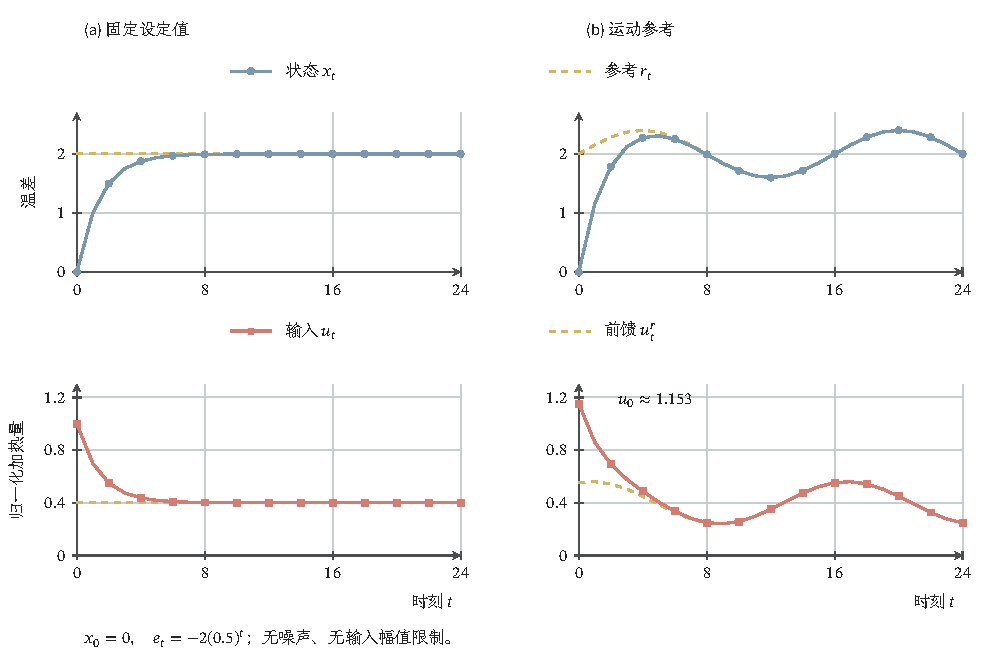
\includegraphics[width=\linewidth]{figures/01-mathematical-preliminaries/05-dynamical-systems-control-decision-and-games/tikz/control/temperature-regulation-tracking.pdf}
  \caption{同一无噪声温度模型、初态$x_0=0$与误差增益$0.3$下的调节和跟踪。
  左列固定$r_t=2$，右列取$r_t=2+0.4\sin(\pi t/8)$；上排比较参考与实际状态，
  下排比较维持参考的前馈与完整输入。两种任务的误差均为$e_t=-2(0.5)^t$，
  但运动参考需要持续变化的前馈。图中输入无幅值限制，右下首个动作超过$1$，
  因而此图不是受限执行器的安全证明。离散点之间连线仅便于阅读。}
  \label{fig:control-temperature-regulation-tracking}
\end{figure*}

误差趋零、误差有界与始终不超过某阈值仍有区别。
无扰动时，$|e_t|=0.5^t|e_0|$既给出收敛，也给出从首步起的范围；
一般多维稳定矩阵可能先放大误差，需要使用$M\rho^t$而不能省掉$M$。
只证明$\sup_t\|\bm e_t\|<\infty$不说明误差是否足够小。
参考位于安全集内也不保证实际状态安全，必须把参考与误差范围相加后再核对约束。

\subsubsection{扰动与模型偏差下的轨迹跟踪}
真实动态与参考规划常有偏差。设实际系统为
$\bm x_{t+1}=(\bm A+\Delta\bm A)\bm x_t+
(\bm B+\Delta\bm B)\bm u_t+\bm d_t$，
名义参考的实现残差为
$\bm\eta_t=\bm A\bm r_t+\bm B\bm u_t^r-\bm r_{t+1}$。
沿用名义前馈加反馈后，误差的完整方程为
\begin{equation}
  \begin{aligned}
  \bm e_{t+1}
  ={}&(\bm F+\Delta\bm A-\Delta\bm B\bm K)\bm e_t\\
     &+\Delta\bm A\bm r_t+\Delta\bm B\bm u_t^r+\bm\eta_t+\bm d_t,
  \qquad \bm F=\bm A-\bm B\bm K.
  \end{aligned}
  \label{eq:control-tracking-model-error}
\end{equation}
偏差既改变误差反馈矩阵，也使原先可实现的参考变成受迫误差来源。
因此只验证名义$\bm F$稳定，还不足以覆盖任意模型误差。

固定一种向量范数及相容矩阵范数，假设$\|\bm F\|\leq\rho<1$，
$\|\Delta\bm A-\Delta\bm B\bm K\|\leq\varepsilon$且
$q:=\rho+\varepsilon<1$。稳定矩阵可以在适当范数中取得收缩界，
但偏差界和以下所有大小必须在同一范数下计算，不能混用欧氏范数数值。
若$\|\bm r_t\|\leq R_0,\|\bm u_t^r\|\leq U_0$，
且$\|\bm\eta_t\|\leq\bar\eta,\|\bm d_t\|\leq\bar d$，令
$D=\|\Delta\bm A\|R_0+\|\Delta\bm B\|U_0+\bar\eta+\bar d$，则
\begin{equation}
  \|\bm e_t\|\leq q^t\|\bm e_0\|
         +\frac{1-q^t}{1-q}D.
  \label{eq:control-tracking-error-bound}
\end{equation}
证明只需由式~\eqref{eq:control-tracking-model-error}取范数，
再展开$\|\bm e_{t+1}\|\leq q\|\bm e_t\|+D$的几何级数。
若受迫项趋零且齐次误差仍稳定，误差也趋零；若受迫项仅有界，
一般只能保证$\limsup_t\|\bm e_t\|\leq D/(1-q)$。
积分器可消除合适模型下的常值输出偏差，不能无条件抵消任意运动参考产生的时变失配。

在精确温度模型中，若$|d_t|\leq0.1$，
则$|e_t|\leq0.5^t|e_0|+0.2(1-0.5^t)$。
若希望误差始终位于$[-\delta,\delta]$，应检查
$|e_0|\leq\delta$及$0.5\delta+0.1\leq\delta$，
而不只报告最终误差界。对前述正弦参考，选择$\delta=0.6$时，
实际状态落在$[1.0,3.0]$，输入落在约$[0.059,0.741]$；
在这个误差范围内，参考加上误差仍满足状态约束，前馈加上反馈也满足输入
约束。这就给出了跟踪与安全同时成立的一组局部条件。
图中的$e_0=-2$不在这个范围，不能套用这项保证。

如果安全控制器把名义动作改为
$\bm u_t=\bm u_t^r-\bm K\bm e_t+\Delta\bm u_t^{\mathrm s}$，
精确模型的误差方程还多出$\bm B\Delta\bm u_t^{\mathrm s}$。
修正有界时可并入误差界；修正逐渐消失时可恢复无扰动的渐近跟踪。
若目标与安全约束冲突，修正可能始终不消失，此时必须保留安全并承认跟踪目标不可实现，
不能同时宣称两项保证。

\section{策略的约束与安全}
\label{sec:control-safety-cbf}

即使控制器能使误差最终变小，纠偏过程中仍可能越界。现在固定允许状态与输入范围，
把每一步可行的动作连接到整段轨迹的安全性，再用这些条件修正调节或跟踪动作。
安全条件决定能选什么，性能准则决定在其中选哪个；二者须分别验证。

\subsection{状态约束下的安全区域}
一个制动系统最终停下，仍可能在停下之前越过位置边界；平均成本很小的随机系统，
也可能有不可接受的少数路径。安全集合（safe set）直接规定允许出现的状态。
对确定性离散闭环$\bm x_{t+1}=F_\kappa(\bm x_t)$，集合$S$安全保持的条件为
\begin{equation}
  F_\kappa(S)\subseteq S.
  \label{eq:control-discrete-invariance}
\end{equation}
从$\bm x_0\in S$出发，应用一步条件得到$\bm x_1\in S$，
归纳便有所有$\bm x_t\in S$。反之，若要求$S$内每个初态均不离开$S$，
特别考察其第一步，就得到上述包含关系。因此它对确定性离散闭环既充分又必要。

例如$x_{t+1}=x_t+u_t$的安全集合为$[0,\infty)$。
反馈$u_t=-1.5x_t$给$x_{t+1}=-0.5x_t$，虽然幅值趋零，
却使任意$x_0>0$在第一步越界；$u_t=-0.5x_t$给$x_{t+1}=0.5x_t$，
既稳定又保持非负。图~\ref{fig:control-stability-safety}保留这一对照，
应观察整段轨迹，而不只看最终状态。原系统能到达负半轴也只说明可达，
不说明所选闭环应当到达那里。
\begin{figure}[htbp]
  \centering
  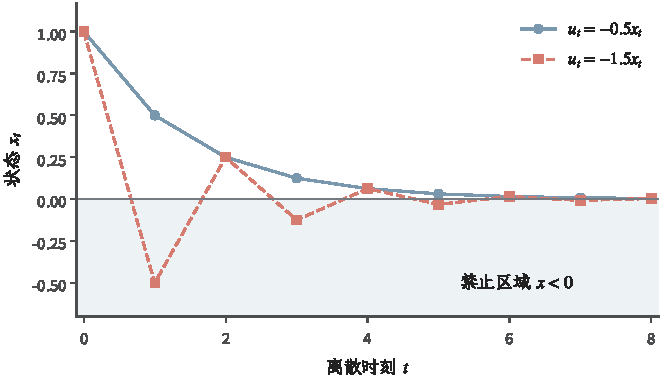
\includegraphics[width=\linewidth]{figures/01-mathematical-preliminaries/05-dynamical-systems-control-decision-and-games/matplotlib/dynamics/stability-safety.pdf}
  \caption{教学系统$x_{t+1}=x_t+u_t$从$x_0=1$出发。
  蓝色圆点采用$u_t=-0.5x_t$，保持$x_t\geq0$；
  红色方点采用$u_t=-1.5x_t$，第一步进入禁止的负半轴后交替衰减。
  两者都渐近稳定，只有前者保持安全集合。灰色区域表示禁止状态。}
  \label{fig:control-stability-safety}
\end{figure}

连续时间还需保证两个观测时刻之间也不越界。考虑控制仿射系统
\begin{equation}
  \dot{\bm x}_t=\bm f(\bm x_t)+\bm G(\bm x_t)\bm u_t,
  \qquad \bm u_t\in U,
  \label{eq:control-affine-system}
\end{equation}
其中$\bm x_t\in\mathbb R^n,\bm u_t\in\mathbb R^m$，
$\bm G(\bm x)\in\mathbb R^{n\times m}$。假设$\bm f,\bm G$局部Lipschitz，
且所选反馈给出存在且唯一的闭环解。以$C^1$函数$h$表示安全集合
\begin{equation}
  S=\{\bm x:h(\bm x)\geq0\}.
  \label{eq:control-safe-set}
\end{equation}
\begin{definition}[正向不变集]
\label{def:control-forward-invariance}
若任意$\bm x_0\in S$所产生的闭环解，在其存在的全部未来时刻均位于$S$，
称$S$对该闭环正向不变（forward invariant）。
\end{definition}
这是定义~\ref{def:dynamical-invariant-limit-sets}在可选择输入的系统中的应用：
本节需要设计使集合保持不变的反馈，而不是只分析已给定规律。
若要说“所有$t\geq0$”，还必须排除有限时间解爆破。

若边界$\partial S=\{h=0\}$光滑且其上$\nabla h\neq\bm0$，
内侧对应$h$增大的方向。Nagumo边界条件要求闭环速度指向内侧或与边界相切：
\begin{equation}
  \nabla h(\bm x)^\top
  [\bm f(\bm x)+\bm G(\bm x)\bm u]\geq0
  \quad\text{当 }h(\bm x)=0.
  \label{eq:control-nagumo-boundary}
\end{equation}
在闭集、正则边界和适定闭环等条件下，它给出正向不变判据。
边界梯度退化时不能机械沿用这条光滑表达，应检查真实切锥。
控制器还需要在接近边界时就限制动作，下面把边界条件扩展到集合附近。

\subsection{安全条件下的可行动作}
函数$h$只用符号区分安全与否，不必等于几何距离。
动作是否安全取决于$h$沿速度的变化，链式法则给出
\[
  L_{\bm f}h(\bm x)=\nabla h(\bm x)^\top\bm f(\bm x),
  \qquad
  L_{\bm G}h(\bm x)=\nabla h(\bm x)^\top\bm G(\bm x).
\]
它们称为\term{Lie导数}（Lie derivative），分别表示无控制漂移与控制方向对
安全函数变化率的贡献。本章的扩展类$\mathcal K$函数指连续、严格递增、
局部Lipschitz且$\alpha(0)=0$的$\alpha:\mathbb R\to\mathbb R$；
例如$\alpha(r)=\gamma r,\gamma>0$。局部Lipschitz条件用于标量比较系统的唯一性。

在安全区域内部，控制器可以允许$h$减小，使状态接近边界，但要限制减小速度；
到达边界$h=0$时，则必须禁止$h$继续减小。下式用$-\alpha(h)$同时表达这两项要求。
\begin{definition}[零化控制屏障函数]
\label{def:control-cbf}
若在包含$S$的开区域$D$中，每个状态都存在$\bm u\in U$使
$L_{\bm f}h(\bm x)+L_{\bm G}h(\bm x)\bm u\geq-\alpha(h(\bm x))$，
则称$h$为该区域上的零化控制屏障函数（control barrier function, CBF）。
其上确界表达为
\begin{equation}
  \sup_{\bm u\in U}
  \{L_{\bm f}h(\bm x)+L_{\bm G}h(\bm x)\bm u\}
  \geq-\alpha(h(\bm x)),
  \label{eq:control-cbf-existence}
\end{equation}
并要求有实际动作满足该阈值；特别是上确界恰等于阈值时，必须能够取到。
\end{definition}
CBF把“留在区域内”变成每个状态可检查的动作不等式。
当$U$紧且动作函数连续时，上确界可取到，数值不等式就足够；
对非紧$U$，若上确界严格大于阈值，也能选到满足阈值的动作，
不必要求无穷大的上确界被取到。真正需要的是以下集合非空：
\begin{equation}
  K_{\mathrm{cbf}}(\bm x)=
  \{\bm u\in U:L_{\bm f}h(\bm x)+L_{\bm G}h(\bm x)\bm u
                      \geq-\alpha(h(\bm x))\}.
  \label{eq:control-cbf-action-set}
\end{equation}
执行器约束已经通过$\bm u\in U$取交集，不能先忽略输入上限设计动作，
再默认饱和后的动作仍符合屏障条件\scite{math-ames2017cbf}

\begin{theorem}[CBF条件保证正向不变]
\label{thm:control-cbf-invariance}
设式~\eqref{eq:control-affine-system}及安全函数满足上述正则条件。
若反馈$\bm u=\kappa(\bm x)$局部Lipschitz，并在包含$S$的开区域$D$中始终满足
$\kappa(\bm x)\in K_{\mathrm{cbf}}(\bm x)$，
则$S$在相应闭环解存在的时间区间内正向不变。
\end{theorem}
\begin{proof}
沿任意闭环解记$r_t=h(\bm x_t)$，链式法则和CBF约束给出
$\dot r_t\geq-\alpha(r_t)$。考虑比较系统
\[
  \dot z_t=-\alpha(z_t),\qquad z_0=r_0\geq0.
\]
$\alpha$局部Lipschitz，比较系统局部解唯一，且$z=0$是平衡解；
从非负初值出发的解不能穿过零点。又因$\alpha$严格递增且$\alpha(0)=0$，
$z_t$留在$[0,z_0]$内，所以比较解在任意有限时间存在。
为验证微分不等式中的$r_t$也不低于$z_t$，在轨迹位于$D$的任一紧时间区间上，
取$\alpha$在两条标量轨迹值域所在紧区间的Lipschitz常数$L$，并令
$q_t=\max\{z_t-r_t,0\}$。在$z_t>r_t$处，
\[
 \dot q_t=\dot z_t-\dot r_t
 \leq-\alpha(z_t)+\alpha(r_t)\leq Lq_t.
\]
正部函数绝对连续，且在其零集上导数几乎处处为零，故这个不等式几乎处处成立。
由$q_0=0$可得$q_t\leq L\int_0^tq_s\,\mathrm ds$；
引理~\ref{lem:action-state-gronwall}遂给出$q_t=0$，即$r_t\geq z_t\geq0$。
因为$D$是包含$S$的开区域，若轨迹离开$S$，必先在$D$中穿过$h=0$进入$h<0$，
与比较不等式矛盾。故在闭环解存在的全部时间内，$\bm x_t\in S$。

对$\alpha(r)=\gamma r$还可以直接验证：
\[
  \frac{\mathrm d}{\mathrm dt}(e^{\gamma t}r_t)
  =e^{\gamma t}(\dot r_t+\gamma r_t)\geq0.
\]
所以$r_t\geq e^{-\gamma t}r_0\geq0$。
当$r=0$时约束退化为$\dot r\geq0$，与边界条件一致。
\end{proof}
这项证明依赖动作约束始终可行、反馈与动态足够规则，以及动作按连续时间模型实际施加。
某一个采样点的动作朝内，不能代替这些沿轨迹的条件。

回到离散温度系统，令$S=[0,3],U=[0,1]$且无噪声。
下一步安全要求$0\leq0.8x+u\leq3$，因此精确的一步安全动作集合为
\begin{equation}
  K_{\mathrm{safe}}(x)
  =[\,\max\{0,-0.8x\},\ \min\{1,3-0.8x\}\,].
  \label{eq:control-temperature-safe-actions}
\end{equation}
对$x\in[0,3]$，下端为$0$，上端至少为$0.6$，所以每个安全状态都有可行动作。
固定目标反馈$u=0.4-0.3(x-2)=1-0.3x$在该区间取值于$[0.1,1]$，
下一状态为$1+0.5x\in[1,2.5]$。它不需要修正就同时实现输入可行、状态安全与趋于$2$。
这个显式包含关系比“反馈稳定”多证明了整个区间的安全保持。

\subsection{可行约束下的反馈修正}
若调节或跟踪给出的名义动作$\bm u_{\mathrm{nom}}$不可行，
可以在每个状态寻找对它修改最小的安全动作：
\begin{equation}
  \begin{aligned}
  \bm u^\ast(\bm x)\in\argmin_{\bm u\in U}\quad&
    \tfrac12(\bm u-\bm u_{\mathrm{nom}})^\top
              \bm H(\bm u-\bm u_{\mathrm{nom}})\\
  \text{s.t.}\quad&
    L_{\bm f}h(\bm x)+L_{\bm G}h(\bm x)\bm u
       \geq-\alpha(h(\bm x)),
  \end{aligned}
  \label{eq:control-cbf-qp}
\end{equation}
其中$\bm H\succ\bm0$规定修改各输入分量的代价。
CBF约束对输入线性；$U$为多面体时这是二次规划（quadratic program, QP），
一般非空闭凸$U$则给出闭凸约束下的二次优化问题。
第~\ref{chap:optimization}章的约束优化工具可用于计算它。
目标只比较当前动作的距离，并不使修正后的整条轨迹保持原LQR成本最优。

\begin{example}[一维积分器上的安全投影]
\label{ex:control-cbf-scalar-projection}
考虑$\dot x_t=u_t$、$S=[0,\infty)$、$h(x)=x$及$\alpha(h)=\gamma h$。
CBF条件为$u\geq-\gamma x$。若$U=\mathbb R,H=1$，解为
\begin{equation}
  u^\ast(x)=\max\{u_{\mathrm{nom}}(x),-\gamma x\}.
  \label{eq:control-cbf-scalar-projection}
\end{equation}
在$x=0.2,\gamma=1$且名义动作恒为$u_{\mathrm{nom}}=-1$时，动作修正为$-0.2$。
持续应用该反馈，状态按$x_t=0.2e^{-t}$接近零而不穿过边界。
若执行器另要求$u\leq-0.5$，此处与$u\geq-0.2$冲突，QP不可行；
安全函数的形式本身不能保证执行器能够提供所需动作。
\end{example}

在上述凸约束下，若可行域非空且闭，正定二次目标在动作范数增大时趋于无穷，
所以极小点存在；严格凸性保证动作唯一。没有闭性时，严格凸只说明已有极小点至多一个，
不能保证下确界取到。即使每个状态上的优化问题都有唯一解，从状态到动作的映射$\bm x\mapsto\bm u^\ast(\bm x)$
也未必局部Lipschitz：约束梯度退化、活跃约束切换或可行域突变可能破坏正则性。
应用不变性定理前，还需按约束资格条件与参数化优化结果核验反馈的规则性。

\begin{example}[圆形障碍外的安全修正]
\label{ex:control-cbf-obstacle}
对平面单积分器$\dot{\bm p}_t=\bm u_t$，
障碍中心为$\bm c$、半径为$r>0$。取
$h(\bm p)=\|\bm p-\bm c\|_2^2-r^2$，安全区域是圆外。
$\alpha(h)=\gamma h$给出
\begin{equation}
  2(\bm p-\bm c)^\top\bm u
  \geq-\gamma(\|\bm p-\bm c\|_2^2-r^2).
  \label{eq:control-cbf-obstacle-constraint}
\end{equation}
在边界$\bm p-\bm c=(r,0)^\top$，名义动作$(-v,0)^\top,v>0$指向障碍内部，
左侧为$-2rv<0$。无其他输入约束且$\bm H=\bm I$时，
QP将动作投影到半空间$2(\bm p-\bm c)^\top\bm u\geq0$，
此处修正为$\bm u^\ast=\bm0$。
若名义动作含有切向分量，投影保留切向分量，只移除向内的法向分量。
停在边界是安全的，却未必能够完成绕行任务。
\end{example}

多个$h_i(\bm x)\geq0$会产生多条动作约束。
每条单独可行，不代表它们与执行器限制联合可行；障碍、制动能力或转向限制可能相互冲突。
加入松弛变量使优化器返回数值解，同时也允许原安全条件被违反，
因而不能再声明原来的硬不变性保证。此时应说明约束冲突后怎样处理、在哪些区域还能恢复安全，或改为保证多大的
越界概率；不能继续使用原先的硬安全结论。
图~\ref{fig:control-barrier-projection}用$(x,u)$平面显示一维投影：
每个固定状态的安全动作是一条竖直半直线，修正沿这条半直线寻找最近点。
\begin{figure}[htbp]
  \centering
  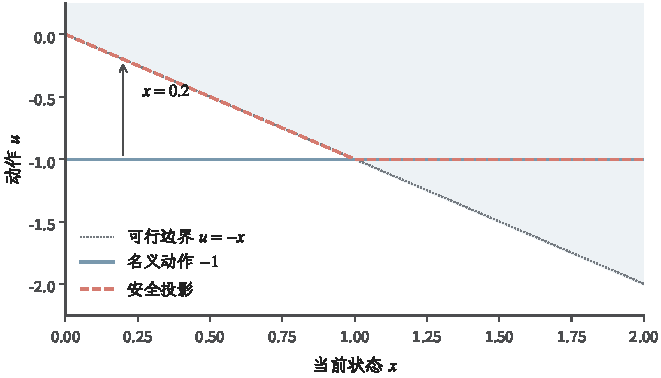
\includegraphics[width=\linewidth]{figures/01-mathematical-preliminaries/05-dynamical-systems-control-decision-and-games/matplotlib/dynamics/barrier-projection.pdf}
  \caption{教学积分器$\dot x_t=u_t$、安全集合$x\geq0$及$\alpha(h)=h$。
  灰色虚线$u=-x$上方为允许动作；蓝色实线为名义动作$u=-1$，
  红色虚线为投影$u^\ast=\max\{-1,-x\}$。
  $x\geq1$处无需修正，$x=0.2$处修正为$-0.2$。
  图中没有额外执行器限制，不能据此判断有限输入范围下的联合可行性。}
  \label{fig:control-barrier-projection}
\end{figure}
\FloatBarrier

对温度模型，使用式~\eqref{eq:control-temperature-safe-actions}的闭区间投影：
\[
  u_t=\min\{u_{\max}(x_t),\max\{u_{\min}(x_t),u_{\mathrm{nom},t}\}\}.
\]
前述正弦跟踪从$x_0=0$出发，名义首个动作为
$0.4+0.4\sin(\pi/8)+0.6\approx1.153$，投影改为$u_0=1$。
于是$x_1=1$，而不是无约束的$1.153$；此时
$e_1=1-[2+0.4\sin(\pi/8)]\approx-1.153$，不再等于$0.5e_0=-1$。
由于每步安全动作集合非空，重复投影仍保持$0\leq x_t\leq3$及$0\leq u_t\leq1$，
但跟踪误差须按增加了修正项的方程重新分析。
目标参考持续要求超出能力的输入时，不能同时保持精确跟踪；
安全投影的“最近”也不等于全时域最优。

\subsection{扰动与离散执行下的安全保证}
若真实连续动态含$\|\bm d_t\|_2\leq\delta$的加性扰动，
最坏方向使安全函数的导数减少至多$\|\nabla h(\bm x)\|_2\delta$。
因此鲁棒充分条件为
\begin{equation}
  L_{\bm f}h+L_{\bm G}h\,\bm u
  \geq-\alpha(h)+\|\nabla h\|_2\delta.
  \label{eq:control-robust-cbf}
\end{equation}
有有效上界的模型误差可并入同一裕量。没有经过验证的误差界时，
任意加一个“安全系数”只是经验缓冲，不能推出鲁棒正向不变性。

离散温度系统若$|w_{t+1}|\leq\delta$，最坏扰动下的安全动作集合为
\begin{equation}
  K_{\mathrm{safe}}^\delta(x)
  =[\,\max\{0,\delta-0.8x\},\
       \min\{1,3-\delta-0.8x\}\,].
  \label{eq:control-temperature-robust-actions}
\end{equation}
当$0\leq\delta\leq0.6$，该集合对所有$x\in[0,3]$非空：
下端不超过$1$，未截断区间宽度$3-2\delta$非负，且上端在$x=3$也不小于零。
若$\delta>0.6$，从$x=3$面对正向最大扰动，即使取最小输入$u=0$也会越界，
所以整个$[0,3]$不能在这类扰动下保持不变。
固定目标的名义反馈产生$1+0.5x+w_{t+1}$，对$\delta\leq0.5$已经落在$[0,3]$，
因而无需修正。高斯噪声没有有限的确定幅值界，不能套用这个逐路径保证；
概率风险要按第~\ref{chap:decision-theory-and-dynamic-risk}章的风险口径另行定义。

数字控制器每隔$\Delta$更新动作，并在区间内保持不变。
采样点满足连续CBF约束，不自动保证区间内部满足，因为状态和安全导数仍在变化。
例如对固定保持动作，若
$g(\bm x,\bm u)=L_{\bm f}h+L_{\bm G}h\,\bm u+\alpha(h)$
在已核验区域内对状态的Lipschitz常数为$L_g$，且速度有界$\|\dot{\bm x}\|\leq M$，
则区间内$g$最多降低$L_gM\Delta$。
采样时预留这一裕量才可保证区间内$g\geq0$；区域与速度界本身也须有效，
不能假定在尚未证明安全的区域外仍成立。

也可以直接构造离散屏障条件
\[
  h(\bm x_{t+1})-h(\bm x_t)\geq-\alpha_{\mathrm d}(h(\bm x_t)),
\]
并要求每个$r\geq0$都有$0\leq\alpha_{\mathrm d}(r)\leq r$。
这样$h(\bm x_t)\geq0$便推出
$h(\bm x_{t+1})\geq h(\bm x_t)-\alpha_{\mathrm d}(h(\bm x_t))\geq0$，
可逐步归纳安全性。常用$\alpha_{\mathrm d}(r)=\gamma r$取$0<\gamma\leq1$。
若离散模型只是连续系统的采样映射，采样点安全仍不等于区间安全，
还需检查采样间轨迹；在预测时域中直接验证整段连续轨迹是另一种办法。

还有一种限制来自\term{相对阶}（relative degree），即对某个输出求导多少次，
当前输入才第一次显式出现。若$L_{\bm G}h=\bm0$，一阶CBF约束不含动作。
例如双积分器$\dot p_t=v_t,\dot v_t=u_t$用
$h(p)=p-p_{\min}$保护位置下界，有$\dot h=v$、$\ddot h=u$，
因此相对阶为$2$。此时需要递归控制更高导数，或把速度与制动距离纳入安全函数。
取$\psi_1=v+k_1h$（$k_1>0$），若再约束
\[
  u+k_1v+k_2\psi_1\geq0,\qquad k_2>0,
\]
则$\dot\psi_1\geq-k_2\psi_1$。在初态同时满足$h\geq0,\psi_1\geq0$、
约束始终可行且闭环适定时，比较原理先保证$\psi_1\geq0$，
再由$\dot h\geq-k_1h$保证$h\geq0$。
新增的速度条件不可省略，执行器幅值也可能使这条高阶约束不可行。

例如$p-p_{\min}=0.1,v=-1$，最大制动加速度为$2$，
最快停止距离$v^2/(2u_{\max})=0.25$已超过剩余距离。
此时位置虽在允许区间，任何允许动作也不能避免后续越界。
安全初态应同时考虑位置与速度；把一阶公式套到$L_{\bm G}h=0$处，
只会得到与输入无关的条件。

CBF还要求用于计算约束的状态信息可靠。
若只有估计值，应先给估计误差集合界或概率模型，再收紧安全集合或构造输出反馈屏障。
把估计均值直接当作真实状态代入，只能验证估计轨迹，
不能从有界误差协方差自动推出真实轨迹的硬安全。

\section{本章小结}
\label{sec:control-theory-summary}

一个可实施策略既要遵守信息时序，也要符合执行器能够改变的方向。
可控、可观测要求处理全部状态方向；可稳定要求输入无法影响的模式已经稳定，可检测要求观测无法区分的误差
模式能够自行衰减。
它们为设计提供结构条件，真正的轨迹行为仍由闭环矩阵、误差动态或Lyapunov不等式决定。
增益还会改变输入幅值和中间阶段的响应，所以不同稳定反馈并非可以不加区别地互换。

在同一温度模型中，固定目标$2$需要平衡输入$0.4$，
再加本章选取的误差反馈，才得到$e_{t+1}=0.5e_t$。
运动参考改用$u_t^r=r_{t+1}-0.8r_t$抵消参考变化，
同一个稳定误差系统便能服务于跟踪。常值扰动、时变扰动和模型偏差改变这一结论：
合适的积分增广可以消除常值输出偏差，对一般的持续扰动，通常只能给出误差范围，
非零随机噪声则应区分均值收敛、协方差有界与路径收敛。

Riccati方法在特定二次成本下选择反馈。有限时域的逐步配方保持二次形式；
确定性无折扣无限时域还需可稳定、成本可检测及权重条件，
才能同时得到稳定化与成本最优性。输出反馈通过估计连接实际信息，
确定性系统中分开设计反馈与观测器的谱结论，以及随机系统中的稳态误差
结论，各有适用条件，
不能把它们推广成任意观测、约束或模型失配下的保证。

安全性约束全过程。对无噪声温度系统，固定目标反馈已经保持
$0\leq u\leq1,0\leq x\leq3$；同一增益的运动参考却可能在初始纠偏时要求过大输入。
一步安全集合或连续屏障约束可以修正动作，但修正后的调节、跟踪与价值必须重新核验。
约束不可行、扰动无有效上界、采样间行为未检查或状态估计不可靠时，
都不能沿用名义安全结论。
第~\ref{chap:decision-theory-and-dynamic-risk}章将进一步比较这些策略的
累计成本、收益与风险；目标可达、误差收敛、轨迹安全和价值最优仍是需要分别回答的问题。

\chapter{策略的价值与优化}
\label{chap:decision-theory-and-dynamic-risk}
\label{chap:policy-value-and-optimization}

把室温调到目标附近，并没有唯一确定怎样加热。快速升温需要较大的输入，缓慢升温则让
人在较长时间内承受温度偏差；有随机扰动时，两项平均成本接近的策略还可能产生不同的
严重后果。第~\ref{chap:control-theory}章已经讨论策略能否实现目标、使误差收敛并保持
安全，本章进一步问：怎样给这些策略的后果计价，怎样算出给定策略的价值，又怎样选择
成本更低的策略？

评价的对象是策略诱导的状态与行动轨迹。确定性模型中，初态和策略可以确定一条轨迹；
随机模型中，它们通常只确定轨迹的分布。因此，要分清一次执行付出的成本、同一策略
多次执行的平均成本，以及对坏尾部的评价。先确定对象和评价准则，才能计算价值；
计算时固定行动规则，优化时才允许改变规则。这个区别也决定了递推中该对行动概率求和，
还是在可选行动中取最小值。

本章以成本最小化为主要约定。若任务使用收益，只需把收益定义为成本的负值，并将
最小化与最大化成套转换。路线选择保留一个可以逐项枚举的轨迹分布，温度模型连接前章
的反馈设计；信息获取和探索例子则说明行动不仅改变物理状态，也会改变以后知道什么。
这些例子最终都要回答同一个问题：在给定信息、模型和评价口径下，哪项可实施策略更合适？

\section{策略的表示与价值}
\label{sec:policy-representation-and-value}

\subsection{策略的行动与信息}
\label{sec:policy-actions-and-information}

加热器每次收到的是一个输入值，控制器需要规定的却是整套选择规则：温度偏低时怎样选，
下一次读数改变后又怎样选。策略（policy）就是按当时已经知道的信息持续选择行动的规则。
它与一条已经执行的行动序列不同；同一策略遇到不同观测，可以产生不同序列。

先用离散时间和有限状态说明信息次序。状态记为$S_t\in\mathcal S$，行动记为
$A_t\in\mathcal A(S_t)$，每个$\mathcal A(s)$均非空。在行动$A_t$发生之前，完整
状态历史为
\[
  H_t=(S_0,A_0,S_1,\ldots,A_{t-1},S_t).
\]
历史依赖随机策略用概率$\pi_t(a\mid h_t)$指定下一行动，满足
$\pi_t(a\mid h_t)\geq0$及$\sum_a\pi_t(a\mid h_t)=1$，并仅支持当前允许行动。
确定性策略将全部质量放在某个行动上。连续行动时使用可测概率核
$\pi_t(\mathrm da\mid h_t)$，而不是对单个实数行动指定密度而忘记可能的原子质量。
策略的随机数在使用时产生，不得包含未来环境噪声的信息。

若策略只读取当前状态，写作$\pi_t(a\mid s)$，称为Markov策略；若规则还不随时间
改变，写作$\pi(a\mid s)$，称为平稳Markov策略。只去掉历史依赖不等于去掉时间依赖：
距离截止时间还有多久，常会改变合理的动作。前章的开环序列、状态反馈和输出反馈，
分别规定了这些规则怎样接入实际系统，见定义
~\ref{def:control-open-loop-state-output-feedback}。

若只能观察$Y_t$，允许信息是
$\mathcal I_t=\sigma(Y_0,A_0,\ldots,A_{t-1},Y_t)$，策略不能直接读取$S_t$。
即使观测与状态同维，也不能把带噪声读数当作真实状态。
第~\ref{chap:dynamical-systems-and-state-estimation}章状态推断给出的条件分布
$b_t(\mathrm ds)=\mathbb P(S_t\in\mathrm ds\mid\mathcal I_t)$汇集了观测历史对当前
状态的认识。在模型已知、该分布连同时间足以预测后续观测和成本时，可以用$b_t$作为
决策的状态；这不是说一次观测$Y_t$本身满足同样条件。

共同温度模型仍为
\begin{equation}
  x_{t+1}=0.8x_t+u_t+w_{t+1},
  \qquad y_t=x_t+v_t.
  \label{eq:policy-temperature-model}
\end{equation}
$x_t$是相对于环境温度的温差，$u_t$是加热量。本章先取
$w_{t+1}=v_t=0$，默认$u_t\in\mathbb R$，不暗加输入限制。目标$r=2$需要平衡输入
$u^r=2-0.8\times2=0.4$。前章的示例状态反馈
\begin{equation}
  u_t=0.4-0.3(x_t-2)
  \label{eq:policy-temperature-feedback}
\end{equation}
使误差$e_t=x_t-2$满足$e_{t+1}=0.5e_t$。这说明无噪声时误差收敛，却还没有给出
这项策略的成本。若恢复观测噪声，式中的$x_t$须可见，或另行设计基于估计的策略；
直接把$y_t$代入得到的是另一项策略。

\subsection{策略诱导的轨迹}
\label{sec:policy-induced-trajectories}

只有策略还不能预测结果：同一“走捷径”的规则，在不同路况模型下产生的终点概率不同。
因此需要把初态、行动选择和环境转移连接起来。取有限时域$t=0,\ldots,H$，
初始分布为$\mu_0$，阶段成本为$c_t(s,a)$，终端成本为$c_H(s)$。
在每段末状态为$s$的历史$h_t$下，要求受控转移满足
\[
  \mathbb P(S_{t+1}=s'\mid H_t=h_t,A_t=a)=P_t(s'\mid s,a).
\]
这个Markov条件说的是给定当前状态和行动后，过去不再提供预测下一状态的额外信息；
成本也已按同样的状态和行动表示。

\begin{definition}[有限Markov决策过程与策略]
\label{def:decision-finite-mdp-policy}
有限状态集$\mathcal S$、各状态的非空有限行动集$\mathcal A(s)$、初始分布$\mu_0$、
受控转移概率$P_t$、阶段成本$c_t$和终端成本$c_H$组成有限时域
\term{Markov决策过程}（Markov decision process, MDP）。
允许策略可以根据全部已有历史随机选择行动$\pi_t(a\mid H_t)$；
只依赖当前状态时为Markov策略，确定选择时记作$a=\pi_t(s)$。
\end{definition}

这里$S_t,A_t$分别承担前章状态和输入的角色，有限MDP是便于求和计算的版本；
温度模型的连续状态不属于有限集合。若真实转移或成本还依赖未记录的过去，
必须补充状态信息，不能只靠给观测改名来获得Markov性质\scite{math-puterman1994mdp}

现在固定策略$\pi$。对一条状态与行动轨迹
$\tau=(s_0,a_0,s_1,\ldots,a_{H-1},s_H)$，链式法则给出
\begin{equation}
  \mathbb P^\pi(\tau)
  =\mu_0(s_0)\prod_{t=0}^{H-1}
    \pi_t(a_t\mid h_t)P_t(s_{t+1}\mid s_t,a_t).
  \label{eq:policy-trajectory-probability}
\end{equation}
每个因子都对应实际生成的一步：先抽初态，再按当前历史选行动，再由环境生成下一状态。
连续状态时用概率核的逐次积分表达同一构造。输出反馈还要插入观测核，并让行动核仅依赖
已经产生的观测历史；边缘化看不见的状态后，才得到控制器所见的数据分布。

沿用两阶段路线任务。起点$s_0$选择“稳妥”会确定到达终端损失$2$的状态；
选择“捷径”以概率$0.8$到达损失$0$的状态，以概率$0.2$到达损失$6$的状态。
起点行动的阶段成本为零。这里两个阶段指起点选择和终点结算，即$H=1$；
终点没有第二次选择。若策略以概率$p$选择捷径，三条轨迹的概率分别为
\[
  1-p,\qquad 0.8p,\qquad 0.2p.
\]
例如$p=1/2$时为$(0.5,0.4,0.1)$。改变$p$改变行动和终点的联合分布，
但没有改变给定行动后的路况概率。策略随机化与环境随机性因此是两个不同来源。

\subsection{轨迹收益与策略价值}
\label{sec:policy-trajectory-return}

轨迹生成后，可以给实际经过的状态和行动逐项计价。令阶段收益
$r_t(s,a)=-c_t(s,a)$、终端收益$r_H(s)=-c_H(s)$。一条实现轨迹的累计成本和收益为
\begin{equation}
  L(\tau)=\sum_{t=0}^{H-1}c_t(s_t,a_t)+c_H(s_H),
  \qquad G(\tau)=-L(\tau).
  \label{eq:policy-trajectory-cost-return}
\end{equation}
二者是轨迹上的数值，不是策略的平均表现。期望准则下，策略成本为
$J^\pi=\mathbb E^\pi[L]$，策略收益为$\mathbb E^\pi[G]=-J^\pi$；
有限空间可用式~\eqref{eq:policy-trajectory-probability}逐条求和。
后文把成本方向的继续价值记为$V$，因此$V$越小越好。

运行到中途，已经支付的成本不再改变，但后续行动仍可比较。对一段末状态为$s$的历史
$h_t$，一般历史策略的继续成本定义为
\begin{equation}
  J_t^\pi(h_t)=
  \mathbb E^\pi_{h_t}
  \left[\sum_{k=t}^{H-1}c_k(S_k,A_k)+c_H(S_H)\right].
  \label{eq:decision-finite-policy-value}
\end{equation}
下标$h_t$表示固定已知历史，再用策略和转移核重新生成后续过程。
即使该历史在某个初始分布下概率为零，也可以通过这些核定义继续过程，
不必对零概率事件直接作比值条件化。Markov策略下，继续过程只依赖时间与末状态，
于是记作$V_t^\pi(s)$；一般历史策略可能在同一状态记住不同经历，不能无条件这样缩写。
过去累计成本加上$J_t^\pi(h_t)$，才是该历史下整条轨迹总成本的条件期望。

无限时域中，若阶段成本时不变且$|c(s,a)|\leq C$，取$0\leq\gamma<1$，定义
\begin{equation}
  V^\pi(s)=
  \mathbb E_s^\pi\left[\sum_{t=0}^{\infty}\gamma^t c(S_t,A_t)\right].
  \label{eq:decision-discounted-value}
\end{equation}
这里$\pi$仍可依赖全部历史，$s$指定起点。几何级数给出
$|V^\pi(s)|\leq C/(1-\gamma)$，保证累计和与期望有意义。
连续状态的二次成本通常无界，需要另证可积性或矩界；不能只因写了折扣就套用该上界。
无折扣的无限累计也可能发散，尤其是系统持续支付维持目标所需的能耗时。

为共同温度模型定义具体成本，取教学权重$\lambda=1$：
\begin{equation}
  c(x,u)=(x-2)^2+\lambda u^2,\qquad c_H(x)=(x-2)^2.
  \label{eq:policy-temperature-cost}
\end{equation}
第一项惩罚舒适偏差，第二项是按加热幅值平方计价的能耗代理，不声称等于未经标定的
实际电费。这里计的是总输入$u$，不是偏移输入$u-0.4$；两种计价会产生不同的最优策略。
阶段收益始终是$-c(x,u)$。从$x_0=0$执行
式~\eqref{eq:policy-temperature-feedback}两次得到
$(u_0,u_1)=(1,0.7)$和$(x_1,x_2)=(1,1.5)$，
这给出了可逐项评价的一条轨迹。固定规则的计算将在
第~\ref{sec:policy-finite-evaluation}节完成，届时才与其他规则比较。

只有一次行动时，$L$退化为损失$\ell(a,Y)$，收益为$-\ell(a,Y)$。
例如同一阳性概率$0.3$，在对称分类损失与高漏诊损失下会对应不同的行动。
概率只描述结果的可能性，还没有包括后果的代价，更不是多步任务中已经累计未来后果的
继续价值。条件风险和Bayes行动的正式求解留在
第~\ref{sec:decision-bayes-rules}节；先固定策略，下一节比较如何汇总它产生的随机成本。

\section{策略的轨迹价值与风险}
\label{sec:decision-risk-criteria-robustness}

\subsection{平均收益与价值波动}

路线策略已经确定，仍有不止一种评价它的办法。固定走稳妥路线的期望损失为$2$；
固定走捷径的期望损失为$0.8\times0+0.2\times6=1.2$。后者的平均收益较高，
却有$20\%$的概率付出损失$6$。比较策略以前，需要明确任务在意平均成本，还是不能
承受某些严重后果。本节先不改变策略，只比较这些评价口径。

设随机轨迹损失$L$可积。期望$\mathbb E[L]$按发生概率线性汇总所有后果；
对应的期望收益为$-\mathbb E[L]$。为了看清均值遗漏的信息，再考虑两个教学方案
\[
  L_{\mathrm{safe}}=1,\qquad
  L_{\mathrm{tail}}=
  \begin{cases}
    0,&\text{概率 }0.95,\\
    20,&\text{概率 }0.05.
  \end{cases}
\]
二者的期望均为$1$，但第二个方案把全部平均损失集中在最差$5\%$的结果中。
这可以理解为两项已经固定的策略所诱导的终端损失，不能用“平均相同”代替“后果相同”。

有二阶矩时，方差$\operatorname{Var}(L)$衡量围绕均值的二次波动。
均值--方差准则为
\[
  \mathbb E[L]+\lambda\operatorname{Var}(L),\qquad \lambda\geq0.
\]
其中$\lambda$表达波动的权重，与温度成本中的输入权重并无必然关系。该准则同时惩罚
高于和低于均值的偏离，意外变好也会增加方差。更重要的是，它未必尊重逐场景的损失
大小：令$L_1$等概率取$0,2$，令$L_2=2$，则$L_1\leq L_2$，但$\lambda>1$时
\[
  \mathbb E[L_1]+\lambda\operatorname{Var}(L_1)=1+\lambda>2
  =\mathbb E[L_2]+\lambda\operatorname{Var}(L_2).
\]
因此，“厌恶波动”和“避免坏尾部”不是同一个要求。

\begin{definition}[相干风险]
\label{def:decision-coherent-risk}
设风险泛函$\rho:L^1(P)\to\mathbb R$按损失越小越好的方向评价。单调性要求
$L\leq L'$几乎处处时$\rho(L)\leq\rho(L')$；平移等变性要求
$\rho(L+m)=\rho(L)+m$，其中$m$为确定常数。凸性要求
\[
  \rho(\tau L+(1-\tau)L')
  \leq\tau\rho(L)+(1-\tau)\rho(L'),\qquad 0\leq\tau\leq1.
\]
若具有单调性、平移等变性、正齐次性
$\rho(\lambda L)=\lambda\rho(L)$（$\lambda\geq0$）和次可加性
$\rho(L+L')\leq\rho(L)+\rho(L')$，称为\term{相干风险}（coherent risk measure）。
\end{definition}

正齐次性和次可加性已经蕴含凸性；单列凸性是为了与后文一般凸风险比较。
这里的$\tau L+(1-\tau)L'$是在同一场景下按比例承担两份损失，不是先掷硬币选一个
方案，再完整承担该方案的损失。策略随机化通常对应后者，不能直接套用这个凸性公式。
期望满足相干风险的各项性质；均值--方差一般不单调，且需要比可积更强的二阶矩条件。

\subsection{尾部损失与风险评价}

\subsubsection{基于分位数的风险价值}

若任务问“至少$95\%$的执行，损失能否控制在某一水平内”，需要的量是损失分位数，
不是方差。
\begin{definition}[风险价值]
\label{def:decision-value-at-risk}
对实值随机损失$L$与$\alpha\in(0,1)$，左$\alpha$分位数为
\begin{equation}
  q_\alpha(L)=\inf\{z\in\mathbb R:\mathbb P(L\leq z)\geq\alpha\}.
  \label{eq:decision-loss-quantile}
\end{equation}
同一量在风险管理中称为\term{风险价值}（value at risk, VaR），记为
$\operatorname{VaR}_\alpha(L)=q_\alpha(L)$。
\end{definition}
它给出一个损失阈值，不说明阈值以上的后果有多严重。在前面的等均值例中，
\[
  \operatorname{VaR}_{0.95}(L_{\mathrm{safe}})=1,\qquad
  \operatorname{VaR}_{0.95}(L_{\mathrm{tail}})=0.
\]
第二式来自$\mathbb P(L_{\mathrm{tail}}\leq0)=0.95$。分位点恰落在零损失的原子上，
不是说损失$20$已经消失。必须说明左分位数约定，否则离散分布的边界容易产生歧义。

VaR单调且平移等变，但一般不次可加。设互斥事件$E_1,E_2$各有概率$0.04$，
令$L_i=\mathbb I\{E_i\}$。在$\alpha=0.95$时，两项VaR均为零，而合计损失以
概率$0.08$取$1$，所以
\[
  \operatorname{VaR}_{0.95}(L_1+L_2)=1
  >\operatorname{VaR}_{0.95}(L_1)+\operatorname{VaR}_{0.95}(L_2)=0.
\]
单独未超过分位概率预算的两项事件，合并后超过了预算。这个反例否定的是一般次可加性，
不排除特定分布族下可以得到更强的结论。

\subsubsection{基于尾部平均的条件风险价值}

知道尾部从哪里开始，还不足以区分“稍微超标”和“严重损失”。
\term{条件风险价值}（conditional value at risk, CVaR）平均最坏的$1-\alpha$
概率质量\scite{math-rockafellar2000cvar}
\begin{definition}[条件风险价值]
\label{def:decision-conditional-value-at-risk}
对$L\in L^1(P)$和$\alpha\in(0,1)$，定义
\begin{equation}
  \operatorname{CVaR}_\alpha(L)
  =\inf_{\eta\in\mathbb R}
    \left\{\eta+\frac{1}{1-\alpha}\mathbb E[(L-\eta)_+]\right\},
  \qquad (z)_+=\max\{z,0\}.
  \label{eq:decision-cvar-optimization}
\end{equation}
\end{definition}
候选阈值$\eta$提高时，第一项直接增加，超过阈值的剩余损失却会减少。
记花括号中的函数为$\phi(\eta)$。正部函数关于$\eta$凸且为$1$-Lipschitz，
因而可以用有界差商交换单侧极限与期望，得到
\[
  \phi'_+(\eta)=1-\frac{\mathbb P(L>\eta)}{1-\alpha},\qquad
  \phi'_-(\eta)=1-\frac{\mathbb P(L\geq\eta)}{1-\alpha}.
\]
凸函数在$\eta$处最小当且仅当$\phi'_-(\eta)\leq0\leq\phi'_+(\eta)$，即
\begin{equation}
  \mathbb P(L<\eta)\leq\alpha\leq\mathbb P(L\leq\eta).
  \label{eq:decision-cvar-quantile-condition}
\end{equation}
所以满足该条件的分位阈值达到最小值。连续分布中两侧导数通常相同；
阈值处有原子时，左右导数不同恰好记录了这部分概率质量。

令$q=q_\alpha(L)$。由$\mathbb P(L>q)\leq1-\alpha\leq\mathbb P(L\geq q)$，
将$\eta=q$代入阈值式并展开，得到
\begin{equation}
  \operatorname{CVaR}_\alpha(L)=
  \frac{\mathbb E[L\mathbb I\{L>q\}]
    +q\bigl((1-\alpha)-\mathbb P(L>q)\bigr)}{1-\alpha}.
  \label{eq:decision-cvar-atomic-tail}
\end{equation}
第一项收入严格超过$q$的全部损失，第二项从$L=q$的原子补足最坏$1-\alpha$质量。
若$\mathbb P(L\geq q)=1-\alpha$，便可写成$\mathbb E[L\mid L\geq q]$；
分布在分位点处连续是保证该质量相等的常见充分条件。未经检查就对整个事件
$\{L\geq q\}$平均，可能纳入过多概率。质量相等不是两个数值相等的必要条件：
例如常数损失的任意尾部平均都等于该常数。

前面的$L_{\mathrm{safe}}$具有$\operatorname{CVaR}_{0.95}=1$，
$L_{\mathrm{tail}}$最坏$5\%$恰是损失$20$，故其
$\operatorname{CVaR}_{0.95}=20$。期望相同、VaR较小都没有否定这一严重尾部。

\begin{example}[分位点原子中的部分尾部]
\label{ex:decision-cvar-partial-atom}
设$L$以概率$0.6,0.3,0.1$分别取$0,2,10$，取$\alpha=0.75$。
由于$\mathbb P(L<2)=0.6<0.75\leq\mathbb P(L\leq2)=0.9$，分位点为$2$。
最坏$25\%$由损失$10$的全部$10\%$质量和损失$2$的部分$15\%$质量组成：
\[
  \operatorname{CVaR}_{0.75}(L)
  =\frac{0.1\times10+0.15\times2}{0.25}=5.2.
\]
若直接对$L\geq2$条件化，得到
$(0.3\times2+0.1\times10)/0.4=4$，平均了$40\%$质量，不是该CVaR。
\end{example}

图~\ref{fig:decision-cvar-threshold}给出同一例子的阈值目标。横轴最优点$2$
是VaR，纵轴最小值$5.2$才是CVaR；两个数在计算中承担不同角色。
\begin{figure}[htbp]
  \centering
  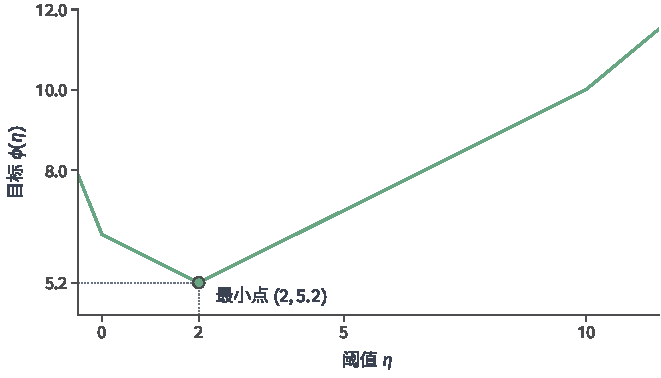
\includegraphics[width=\linewidth]{figures/01-mathematical-preliminaries/05-dynamical-systems-control-decision-and-games/matplotlib/decision-cvar-threshold/figure.pdf}
  \caption{教学分布$P(L=0)=0.6$、$P(L=2)=0.3$、$P(L=10)=0.1$在
  $\alpha=0.75$下的阈值目标$\phi(\eta)=\eta+4\mathbb E[(L-\eta)_+]$。
  绿色折线的最小点为$(2,5.2)$；阈值$2$与尾部平均$5.2$不能混用。}
  \label{fig:decision-cvar-threshold}
\end{figure}

\subsubsection{基于风险包络的尾部评价}

同一个CVaR也可以不用移动阈值，而改成对坏结果增加评价权重。对$L\in L^1(P)$，
\begin{equation}
  \operatorname{CVaR}_\alpha(L)
  =\sup_\zeta\left\{\mathbb E_P[\zeta L]:
    0\leq\zeta\leq\frac{1}{1-\alpha},\quad\mathbb E_P[\zeta]=1\right\}.
  \label{eq:decision-cvar-risk-envelope}
\end{equation}
$\zeta$是相对于原分布的密度比；这些允许密度组成风险包络。
上界$1/(1-\alpha)$阻止全部评价质量压到概率小于$1-\alpha$的事件上。

有限分布中，令结果$i$的原概率为$p_i$、重加权概率为$q_i=p_i\zeta_i$，
右侧变为线性规划
\[
  \max_{\bm q}\sum_iq_iL_i
  \quad\text{s.t.}\quad
  0\leq q_i\leq\frac{p_i}{1-\alpha},\qquad \sum_iq_i=1.
\]
若较小损失仍有质量而较大损失尚未达到上界，将一小部分质量转移到较大损失不会降低
目标。反复转移便得到从最大损失开始填充的解；最后一个损失只取部分质量时，
正是式~\eqref{eq:decision-cvar-atomic-tail}的边界补足。

一般可积分布也能直接证明等式，不必只诉诸形式对偶。对任意可行$\zeta$和$\eta$，
\[
  \mathbb E[\zeta L]
  =\eta+\mathbb E[\zeta(L-\eta)]
  \leq\eta+\frac{\mathbb E[(L-\eta)_+]}{1-\alpha}.
\]
对$\eta$取下确界，说明任意可行密度的加权期望都不超过CVaR。
反向令$q=q_\alpha(L)$，
$b=(1-\alpha)-\mathbb P(L>q)$。若$\mathbb P(L=q)>0$，取
\[
  \zeta^\star=
  \frac{\mathbb I\{L>q\}}{1-\alpha}
  +\frac{b\,\mathbb I\{L=q\}}{(1-\alpha)\mathbb P(L=q)}.
\]
分位条件保证$0\leq b\leq\mathbb P(L=q)$，故密度满足上界且期望为$1$。
若$\mathbb P(L=q)=0$，则$b=0$，只保留第一项。计算
$\mathbb E[\zeta^\star L]$得到原子尾部公式，所以上确界达到CVaR。

例~\ref{ex:decision-cvar-partial-atom}中，损失$10$的原质量$0.1$至多放大为$0.4$，
剩余$0.6$放到损失$2$，重加权为$(0,0.6,0.4)$。
\begin{figure}[htbp]
  \centering
  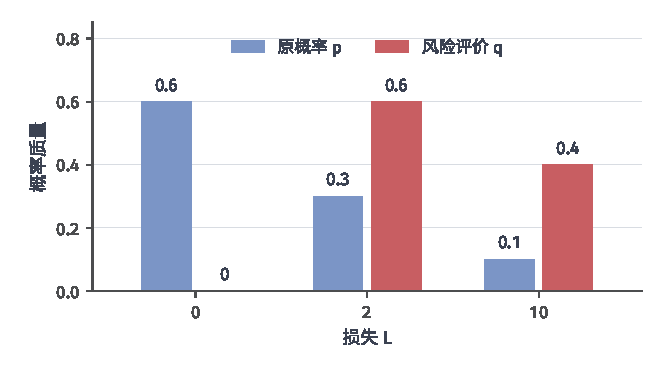
\includegraphics[width=\linewidth]{figures/01-mathematical-preliminaries/05-dynamical-systems-control-decision-and-games/matplotlib/decision-cvar-reweighting/figure.pdf}
  \caption{损失$0,2,10$的名义概率为$(0.6,0.3,0.1)$，CVaR$_{0.75}$的约束为
  $q_i\leq4p_i$和$\sum_iq_i=1$。最优重加权$(0,0.6,0.4)$的期望为$5.2$。
  蓝色为名义质量，红色为对偶最优质量；真实发生概率并未因评价重加权而改变。}
  \label{fig:decision-cvar-reweighting}
\end{figure}

CVaR的相干性质也可从阈值式逐项核对。$L\leq L'$使每个阈值下的正部期望不增，
取下确界得到单调性。将$L+m$的阈值写成$\eta=\bar\eta+m$，便得
$\operatorname{CVaR}_\alpha(L+m)=\operatorname{CVaR}_\alpha(L)+m$。
对$t>0$令$\eta=t\bar\eta$得到正齐次性，$t=0$直接由零损失验证。
又由于
\[
  (L_1+L_2-\eta_1-\eta_2)_+
  \leq(L_1-\eta_1)_++(L_2-\eta_2)_+,
\]
先以$\eta_1+\eta_2$评价合计损失，再分别对两个阈值取下确界，得到次可加性，
继而得到凸性。这些性质都不要求损失分布连续。

这个包络是由既定概率和尾部水平$\alpha$规定的评价权重集合。模型不确定性则问
真实生成机制可能是哪一个分布。二者都能写成最坏期望，但一般不是同一集合，
更不能把重加权结果当作重新估计出的真实事故概率。

\subsection{概率约束与模型不确定性}

有些要求不是把风险再加进目标，而是排除违规概率过大的策略。固定策略产生损失$L$，
给定阈值$b$和$\varepsilon\in(0,1)$，\term{机会约束}（chance constraint）为
\begin{equation}
  \mathbb P(L>b)\leq\varepsilon.
  \label{eq:decision-chance-constraint}
\end{equation}
它控制超标是否发生，不区分超标幅度。由于
$\operatorname{VaR}_{1-\varepsilon}(L)\leq
\operatorname{CVaR}_{1-\varepsilon}(L)$，
条件$\operatorname{CVaR}_{1-\varepsilon}(L)\leq b$蕴含此机会约束。
反向一般不成立，小概率违规的损失可以很大。

必须把违规事件写清楚。温度任务可以限制终端$\{x_H>3\}$、某时刻$\{x_t>3\}$，
也可以限制整段$\{\exists t\leq H:x_t\notin[0,3]\}$。若每个时刻违规概率至多为
$\varepsilon_t$，并集界只给出整段违规概率不超过$\sum_{t=0}^H\varepsilon_t$；
各时刻都不超过$\varepsilon$，不自动使整段也不超过$\varepsilon$。
期望舒适成本很小同样不能替代这些事件保证。

加入输入限制$0\leq u\leq1$和状态限制$0\leq x\leq3$时，先检查可行性。
无噪声下，任意$x\in[0,3]$取$u=0$即可留在区间内，但共同反馈
$u=1-0.3x$还需单独核验：它在区间上取$[0.1,1]$，且下一状态
$x'=0.5x+1\in[1,2.5]$，因此可行。为演示有界扰动下的逐路径安全，
这里将第~\ref{chap:control-theory}章“策略的实现与轨迹控制”中用于矩计算的高斯噪声
改为两点分布；动力学和反馈不变，但噪声假设不同。若$w_{t+1}$独立同分布、等概率取$\pm0.1$，
同一反馈有$x'\in[0.9,2.6]$，仍可保持该区间。这一例取状态完全可见，过程噪声
独立于初态及策略私有随机数。若另有观测噪声$v_t$独立同分布且等概率取$\pm0.05$，
并与过程噪声、初态和私有随机数相互独立，则必须重新检查具体输出反馈；
不能将状态反馈的保证照搬。无界高斯扰动则不能由这种有界输入保证逐路径不越界。

若转移机制由未知$\theta\in\Theta$决定，固定策略的最坏期望是
$\sup_{\theta\in\Theta}\mathbb E^\pi_{P_\theta}[L]$。
\term{分布鲁棒优化}（distributionally robust optimization, DRO）使用候选分布集
$\mathcal P$，相应的评价为$\sup_{Q\in\mathcal P}\mathbb E^\pi_Q[L]$。
距离、矩条件或散度可以规定$\mathcal P$，但集合如何构造和真实分布落入集合的置信保证
仍须分别论证；分布比较工具本身不会自动给出覆盖保证。优化阶段再对允许策略取下确界，
不能在固定策略评价中提前改变行动。

以$L_{\mathrm{safe}}$和$L_{\mathrm{tail}}$为例，$b=10,\varepsilon=0.05$时，
两者违规概率为$0$和$0.05$，都满足机会约束；CVaR$_{0.95}$却为$1$和$20$。
若第二项损失$20$的概率只知$p\in[0.02,0.08]$，最坏期望为
$\max_p20p=1.6$，逐路径最坏损失为$20$，而机会约束在整个集合上不成立，
因为$p=0.08$也被允许。这些数分别描述尾部平均、事故概率、最坏模型平均和路径上界。

有限样本空间中，非空闭候选集位于紧致概率单纯形内，线性期望必达到最大值。
若集合排除某些结果，保证也只覆盖其允许支持。交换策略的$\inf$与模型的$\sup$，
或把内层写成无间隙的对偶，还需凸性、紧致性、连续性或相应约束资格；
最坏分布存在并不够。随机波动、参数估计误差和模型歧义由此得到区分。

\subsection{逐时信息下的动态风险}
\label{sec:decision-dynamic-risk-time-consistency}

\subsubsection{静态尾部评价与偏好反转}

从起点评价整条轨迹，与到达某个分支后重新评价剩余损失，是两个不同操作。
期望有塔式性质把二者连接起来，静态CVaR一般没有同样的关系。
考虑一棵两阶段树：起点等概率进入$N$和$B$，$N$的损失固定为$2$；
在$B$可以预先承诺固定方案$F$或随机方案$R$，
\[
  L_F=3.5,\qquad
  L_R=
  \begin{cases}
    0,&\text{条件概率 }1/2,\\
    4,&\text{条件概率 }1/2.
  \end{cases}
\]
先分别评价这两项承诺策略。承诺$F$时，起点损失以相同概率取$2,3.5$，
所以$\operatorname{CVaR}_{0.5}(L^F)=3.5$。承诺$R$时，起点损失以概率
$1/4,1/2,1/4$取$0,2,4$，故
\[
  \operatorname{CVaR}_{0.5}(L^R)
  =\frac{(1/4)\times4+(1/4)\times2}{1/2}=3.
\]
静态评价因此偏好$R$。真正到达$B$后，只在该条件分布内重算同一水平的CVaR，
却有
\[
  \operatorname{CVaR}_{0.5}(L_F\mid B)=3.5,\qquad
  \operatorname{CVaR}_{0.5}(L_R\mid B)=4,
\]
排序反转。起点评价时，$N$的损失占用了静态尾部的一部分；条件化后，未到达的$N$
已经排除。反转不是算错，而是整条轨迹的尾部与当前分支的尾部并非同一批结果。

\begin{table*}[htbp]
  \centering
  \begin{tabularx}{\linewidth}{XccX}
    \toprule
    评价口径 & 承诺$F$ & 承诺$R$ & 比较依据\\
    \midrule
    初始静态$\operatorname{CVaR}_{0.5}$ & $3.5$ & $3$ & 整棵树最坏一半的损失\\
    到达$B$后的条件$\operatorname{CVaR}_{0.5}$ & $3.5$ & $4$ & $B$内最坏一半的损失\\
    两层嵌套$\operatorname{CVaR}_{0.5}$ & $3.5$ & $4$ & 先评价子节点，再评价节点风险\\
    \bottomrule
  \end{tabularx}
  \caption{同一两阶段分布的三种评价。根节点等概率到达$N$或$B$，$N$固定损失为$2$。
  前两行发生偏好反转；第三行使用下节定义的嵌套目标，其数值不等于静态总损失CVaR。}
  \label{tab:decision-static-conditional-nested}
\end{table*}

\subsubsection{条件风险与时间一致性}

要在每次增加信息后按同一规则评价剩余损失，可以明确规定：下一节点先给出风险值，
当前节点再汇总这些值。令$\mathcal F_0\subseteq\cdots\subseteq\mathcal F_H$
为逐时增长的信息；阈值等评价参数只能使用当时已知的信息。
\begin{definition}[一步条件风险映射]
\label{def:decision-conditional-risk-mapping}
在同一概率空间上，一步\term{条件风险映射}（conditional risk mapping）
\[
  \rho_t:L^\infty(\mathcal F_{t+1})\longrightarrow L^\infty(\mathcal F_t)
\]
把下一时刻可知的有界随机损失转成当前信息下的风险。输入与输出均按几乎处处相等的
等价类理解。
\end{definition}
常用条件为单调性、当前信息下的平移等变性和归一化：
\begin{align}
  Z\leq Z'&\ \Longrightarrow\ \rho_t(Z)\leq\rho_t(Z'),
  \label{eq:decision-conditional-risk-monotonicity}\\
  \rho_t(Z+M)&=\rho_t(Z)+M,\qquad M\in L^\infty(\mathcal F_t),
  \label{eq:decision-conditional-risk-translation}\\
  \rho_t(0)&=0.\notag
\end{align}
条件期望满足这些条件。有限树上逐节点评价的映射还具有局部性：若事件
$E\in\mathcal F_t$，只改变$E$之外的未来损失，不改变$E$内的评价。
一般条件模型使用节点解释时也须保持这种信息适应性。

条件CVaR为
\begin{equation}
  \operatorname{CVaR}_{\alpha,t}(Z)
  =\operatorname*{ess\,inf}_{\eta\in L^\infty(\mathcal F_t)}
    \left\{\eta+\frac{1}{1-\alpha}
      \mathbb E[(Z-\eta)_+\mid\mathcal F_t]\right\}.
  \label{eq:decision-conditional-cvar}
\end{equation}
$\eta$可随当前历史改变，不能偷看未来结果。
记花括号中的$\mathcal F_t$可测随机变量为$\Phi_\eta$。
这里的本质下确界（essential infimum）是在几乎处处大小关系下最大的共同下界：
它是$\mathcal F_t$可测的随机变量$U$，对每个$\eta$都有$U\leq\Phi_\eta$几乎处处；
任何同样对每个$\eta$满足$V\leq\Phi_\eta$的$\mathcal F_t$可测随机变量$V$，
都必须满足$V\leq U$几乎处处。
因此结果仍随当前历史变化，并不是对全部历史再取一个常数最小值。
这个定义直接在随机变量的几乎处处等价类之间比较，避免把不可数多个版本逐点取下确界时的可测性问题藏起来。
有限概率树上，就是在每个当前节点对其条件分布使用静态阈值公式。
例如固定前例的承诺$R$，在节点$N$与$B$得到的条件风险分别为$2$与$4$。

\begin{definition}[嵌套动态风险]
\label{def:decision-nested-dynamic-risk}
设$C_t\in L^\infty(\mathcal F_t)$为当前已知的有界损失，给定一步映射$(\rho_t)$，
由终端向前定义
\begin{align}
  \mathcal R_H(C_H)&=C_H,\notag\\
  \mathcal R_t(C_t,\ldots,C_H)
  &=C_t+\rho_t\bigl(\mathcal R_{t+1}(C_{t+1},\ldots,C_H)\bigr).
  \label{eq:decision-nested-dynamic-risk}
\end{align}
称为\term{嵌套动态风险}（nested dynamic risk）。
\end{definition}
这里当前成本在风险映射外，是因为它已经属于$\mathcal F_t$。
若成本$\widetilde C_{t+1}$到下一时刻才揭晓，则应写成
\[
  \widetilde{\mathcal R}_t
  =\rho_t(\widetilde C_{t+1}+\widetilde{\mathcal R}_{t+1}).
\]
随机行动尚未抽取时，依赖该行动的阶段成本也属于尚未揭晓的量，不能无条件提出。

\begin{definition}[递归意义下的时间一致性]
\label{def:decision-time-consistency}
动态风险族$(\mathcal R_t)$具有\term{时间一致性}（time consistency），是指对每个
$t<H$、任意两组从$t+1$开始的有界适应损失和同一当前损失$C_t$，只要
$\mathcal R_{t+1}(C_{t+1:H})\leq\mathcal R_{t+1}(C'_{t+1:H})$几乎处处成立，
就有$\mathcal R_t(C_t,C_{t+1:H})\leq\mathcal R_t(C_t,C'_{t+1:H})$几乎处处成立。
\end{definition}
它要求下一时刻每个可能历史上的共同排序在当前仍被保留，而不是要求某个单一实现
总能沿用起点的无条件排序。嵌套结构下，若每个$\rho_t$单调，则
\[
  C_t+\rho_t\bigl(\mathcal R_{t+1}(C_{t+1:H})\bigr)
  \leq
  C_t+\rho_t\bigl(\mathcal R_{t+1}(C'_{t+1:H})\bigr),
\]
正是所需结论。相同当前损失这个条件不可删除，否则当前多付的成本本身就可能逆转比较。

回到两节点例，先固定承诺$F$或$R$。在$B$分别得到风险值$3.5$或$4$，
在$N$均为$2$；根节点再对这两个等概率节点值计算CVaR$_{0.5}$，
得到$3.5$或$4$。所以嵌套评价偏好$F$，静态评价偏好$R$。
递归结构保证了上述时间一致性，但没有把两个不同目标变成同一目标的两种算法。

\section{策略的轨迹价值计算}
\label{sec:policy-value-evaluation}

\subsection{有限时域下的价值递推}
\label{sec:policy-finite-evaluation}

固定策略后，价值计算不再选择行动，而是把该规则可能产生的未来后果逐层汇总。
有限时域从终端开始最直接：$V_H^\pi(s)=c_H(s)$。对于给定Markov策略，
先对下一状态条件化，再按已经指定的行动概率平均，得到
\begin{equation}
  V_t^\pi(s)=\sum_a\pi_t(a\mid s)
  \left[c_t(s,a)+\sum_{s'}P_t(s'\mid s,a)V_{t+1}^\pi(s')\right].
  \label{eq:decision-policy-bellman}
\end{equation}
这就是固定策略的Bellman评价式。若下一时刻的价值已算出，一次矩阵求和即可把
时刻$t$的价值算出；没有任何$\min_a$。

其依据是塔式法则。把累计和拆成$c_t(S_t,A_t)$与后续和，在$S_t=s,A_t=a$
下对后续和条件化，其期望为
$\sum_{s'}P_t(s'\mid s,a)V_{t+1}^\pi(s')$；
再对$\pi_t(a\mid s)$求和，得到上式。归纳到$t=0$后，
$J^\pi=\sum_s\mu_0(s)V_0^\pi(s)$。对一般历史策略，同样的证明给出
\[
  J_t^\pi(h_t)=\sum_a\pi_t(a\mid h_t)
  \left[c_t(s,a)+\sum_{s'}P_t(s'\mid s,a)
    J_{t+1}^\pi(h_t,a,s')\right].
\]
只有当继续规则与所需预测信息都由当前状态概括时，才可把$J_t^\pi(h_t)$缩写为
$V_t^\pi(s)$。Markov环境不意味着任意历史策略本身自动变成Markov策略。

在路线例中，固定以概率$p$走捷径的策略有
\[
  V_0^\pi(s_0)=(1-p)\times2+p(0.8\times0+0.2\times6)=2-0.8p.
\]
$p=1/2$给出$1.6$。这与按三条轨迹概率$(0.5,0.4,0.1)$直接求和一致。
递推省去了枚举长轨迹的代价，却没有改变评价对象。

\begin{example}[温度策略的两步成本]
\label{ex:policy-temperature-evaluation}
取式~\eqref{eq:policy-temperature-model}无噪声、$x_0=0,H=2$，
并按式~\eqref{eq:policy-temperature-cost}计价。固定反馈
$u_t=0.4-0.3(x_t-2)$得到
$(x_0,x_1,x_2)=(0,1,1.5)$、$(u_0,u_1)=(1,0.7)$。
由终端向前，
\begin{align*}
  V_2^\pi(1.5)&=0.25,\\
  V_1^\pi(1)&=1+0.49+0.25=1.74,\\
  V_0^\pi(0)&=4+1+1.74=6.74.
\end{align*}
舒适偏差合计$4+1+0.25=5.25$，输入平方合计$1+0.49=1.49$。
另一项固定策略始终取$u_t=0.4$，产生$(0,0.4,0.72)$，其成本为
\[
  4+1.6^2+1.28^2+0.4^2+0.4^2=8.5184.
\]
其中舒适成本为$8.1984$，输入成本为$0.32$。所以在这个初态、两步时域和给定权重下，
反馈策略用更多输入换来更小的总成本；对应累计收益为$-6.74$和$-8.5184$。
这个比较只涉及两项指定策略，并没有证明第一项在所有策略中最优。
\end{example}

图~\ref{fig:policy-temperature-comparison}将上述评价并列展示：状态更快接近目标，
并不意味着每一项成本都较低。反馈增加了输入成本，但在这两步内节省了更多舒适成本。
\begin{figure*}[htbp]
  \centering
  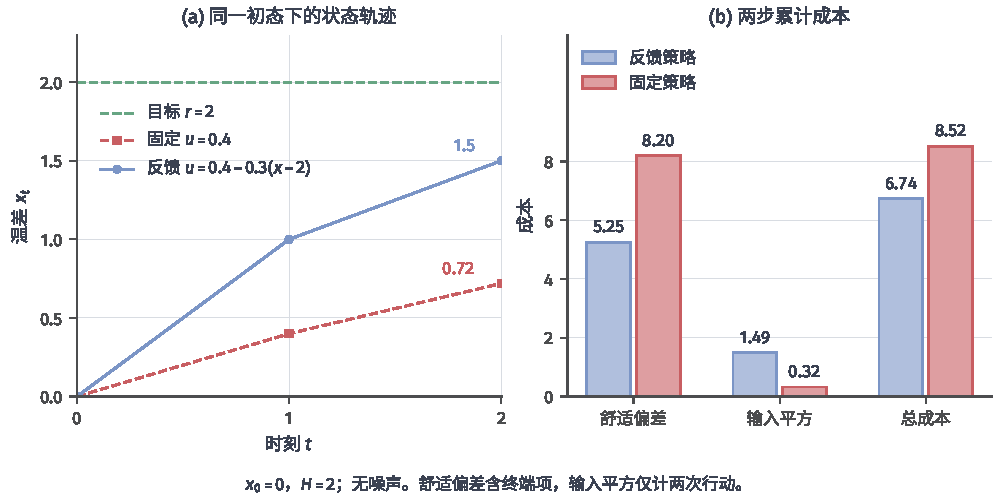
\includegraphics[width=\linewidth]{figures/01-mathematical-preliminaries/05-dynamical-systems-control-decision-and-games/matplotlib/policy-temperature-comparison/figure.pdf}
  \caption{共同温度模型下两项固定策略的比较。左图连接离散时刻的状态，绿色虚线为
  目标温差$2$；连线仅用于辨认轨迹，不表示额外的连续时间模型。右图按
  $c(x,u)=(x-2)^2+u^2$和终端成本$(x-2)^2$累计，柱顶数值保留两位小数。
  反馈的精确总成本为$6.74$，固定输入的总成本为$8.5184$。先分别求值再比较，
  并未在每一步重新选择最优行动。}
  \label{fig:policy-temperature-comparison}
\end{figure*}

恢复随机扰动后，同一反馈诱导轨迹分布而非上述单一路径。若成本可积，
可以沿条件分布求期望；不能只把噪声取均值零后代回非线性的平方成本。
例如$\mathbb E[(x-r)^2]=(\mathbb E[x]-r)^2+\operatorname{Var}(x)$，
漏掉方差项就低估了舒适成本。

\subsection{无限折扣时域下的价值计算}
\label{sec:policy-discounted-evaluation}

有限时域有一个可以启动反向计算的终端，无限时域则没有最后一步。
折扣和有界成本使远期影响可控，由此可把评价转化为固定点计算。
以下取有限状态行动、时不变转移、$|c(s,a)|\leq C$、
$0\leq\gamma<1$和给定的平稳Markov策略$\pi$。定义
\[
  c^\pi(s)=\sum_a\pi(a\mid s)c(s,a),\qquad
  P^\pi(s,s')=\sum_a\pi(a\mid s)P(s'\mid s,a),
\]
以及固定策略评价算子
\begin{equation}
  (T^\pi V)(s)=c^\pi(s)+\gamma\sum_{s'}P^\pi(s,s')V(s').
  \label{eq:policy-discounted-evaluation-operator}
\end{equation}
由$P^\pi(s,s')$组成的矩阵每行非负且和为$1$，所以对任意两个价值函数，
\[
  |(T^\pi V)(s)-(T^\pi W)(s)|
  \leq\gamma\sum_{s'}P^\pi(s,s')|V(s')-W(s')|
  \leq\gamma\lVert V-W\rVert_\infty.
\]
取状态最大值便得到$\gamma$-压缩。有限维最大范数空间完备，压缩映射定理给出
唯一固定点。另一方面，折扣成本的绝对和不超过$C/(1-\gamma)$，
可合法拆出第一项并条件化，得到$V^\pi=T^\pi V^\pi$。
因此这个唯一固定点正是指定策略的期望累计成本，不是最优成本。

从任意$V^{(0)}$出发令$V^{(k+1)}=T^\pi V^{(k)}$，有
\begin{equation}
  \lVert V^{(k)}-V^\pi\rVert_\infty
  \leq\gamma^k\lVert V^{(0)}-V^\pi\rVert_\infty.
  \label{eq:policy-evaluation-iteration-error}
\end{equation}
若取$V^{(0)}=0$，右侧可用$\gamma^kC/(1-\gamma)$替代。
不知$V^\pi$时，也可用可计算残差
\[
  \lVert V-V^\pi\rVert_\infty
  \leq\frac{\lVert T^\pi V-V\rVert_\infty}{1-\gamma},
\]
因为三角不等式和压缩性给出
$\lVert V-V^\pi\rVert_\infty\leq
\lVert V-T^\pi V\rVert_\infty+\gamma\lVert V-V^\pi\rVert_\infty$。
这提供停止评价迭代的误差证书。

将$c^\pi(s),V^\pi(s)$排列为列向量$\bm c^\pi,\bm V^\pi$，以
$P^\pi(s,s')$为元素组成矩阵$\bm P^\pi$，则
\[
  \bm V^\pi=(\bm I-\gamma\bm P^\pi)^{-1}\bm c^\pi
  =\sum_{j=0}^\infty\gamma^j(\bm P^\pi)^j\bm c^\pi.
\]
无穷级数在最大范数下收敛，故逆矩阵存在。单状态例中，
若策略每步以概率$1/4$选择成本$4$的行动，其余选择成本$0$的行动，
则$c^\pi=1$；$\gamma=0.9$时$V^\pi=10$，从零开始迭代得到
$V^{(k)}=10(1-0.9^k)$。这里平均的是固定行动分布；
若把每步成本改成两行动中较小的$0$，算出的已是另一个优化问题。

非平稳或一般历史策略仍有定义良好的有界折扣价值，但其继续规则可能随时间或历史变化，
不能直接使用这个单一平稳算子。可以保留时间、扩充状态，或对有限截断时域评价后
控制余项。连续状态无界二次成本也需要另行选择函数空间与矩条件。

\subsection{风险评价下的价值计算}

\subsubsection{嵌套风险下的递推计算}
\label{sec:policy-nested-risk-evaluation}

先固定确定性Markov策略$a=\pi_t(s)$。若当前状态确实包含风险评价所需的信息，
一步风险映射可写为$\rho_{t,s,a}$，它作用于按$P_t(\cdot\mid s,a)$分布的下一状态。
从终端开始计算
\[
  V_H^{\pi,\rho}(s)=c_H(s),\qquad
  V_t^{\pi,\rho}(s)
  =c_t(s,\pi_t(s))+
    \rho_{t,s,\pi_t(s)}\bigl(V_{t+1}^{\pi,\rho}(S_{t+1})\bigr).
\]
其含义与定义~\ref{def:decision-nested-dynamic-risk}完全一致：先接受后续节点的
评价，再按当前节点风险汇总。策略仍固定，不从其他行动中挑更小的一个。

随机策略需要多说明一层。采取行动之前，$A_t$尚未揭晓；
可在联合条件分布
$\pi_t(a\mid s)P_t(s'\mid s,a)$上，对行动和下一状态一起评价：
\begin{equation}
  V_t^{\pi,\rho}(s)=
  \rho^\pi_{t,s}\bigl(c_t(s,A_t)+V_{t+1}^{\pi,\rho}(S_{t+1})\bigr).
  \label{eq:policy-joint-action-risk-evaluation}
\end{equation}
这里$\rho^\pi_{t,s}$的输入是$(A_t,S_{t+1})$上的随机损失，连当前阶段成本也必须
放在映射内。另一种明确可定义的目标，是先对每个已选行动的环境后果计算风险，
再对行动随机化使用期望：
\[
  \overline V_t^{\pi,\rho}(s)=\sum_a\pi_t(a\mid s)
    \left[c_t(s,a)+\rho_{t,s,a}
      \bigl(\overline V_{t+1}^{\pi,\rho}(S_{t+1})\bigr)\right].
\]
这个公式不是从前式用线性性推出来的，而是改变了行动随机性的评价口径。
路线策略$p=1/2$时，联合损失概率为$0.4$取$0$、$0.5$取$2$、$0.1$取$6$，
联合CVaR$_{0.9}$为$6$；先分别算行动的CVaR再平均，得到
$\tfrac12\times2+\tfrac12\times6=4$。期望下两种次序相同，非线性风险下通常不同。

误差控制依靠单调性和平移等变性，而不依靠线性性。设有限状态上的
$\lVert V-W\rVert_\infty\leq\delta$，则
$W(S')-\delta\leq V(S')\leq W(S')+\delta$，因此
\[
  \rho_{s,a}(W(S'))-\delta
  \leq\rho_{s,a}(V(S'))
  \leq\rho_{s,a}(W(S'))+\delta.
\]
每个映射在最大范数下非扩张。有限时域中一次评价误差不会被单步放大；
若第$t$步另引入至多$\epsilon_t$的数值误差，则反向传播后的初始误差至多为
终端误差加$\sum_{t=0}^{H-1}\epsilon_t$。

无限时域可明确选用“折扣后续风险值”的递归目标。固定确定策略的算子为
\[
  (T^\pi_\rho V)(s)
  =c(s,\pi(s))+\gamma\rho_{s,\pi(s)}(V(S')).
\]
归一化、单调和平移等变保证它把有界向量映到有界向量，且为$\gamma$-压缩，
因而有唯一固定点，迭代误差与残差界分别为
$\gamma^k\lVert V^{(0)}-V^{\pi,\rho}\rVert_\infty$和
$\lVert T^\pi_\rho V-V\rVert_\infty/(1-\gamma)$。
后续风险乘$\gamma$是本目标的明确约定；对CVaR等正齐次风险，它也等于
$\rho_{s,\pi(s)}(\gamma V(S'))$。一般凸风险不一定允许把$\gamma$移入或移出。
若使用随机行动的联合目标
$\rho^\pi_s(c(s,A)+\gamma V(S'))$，相同非扩张论证仍给出$\gamma$-压缩，
但它是该联合目标自己的固定点，不能与前一个目标混称。

上述证明中的$V,W$是有限状态上的实际向量。推广到一般$L^\infty$等价类时，
还须保证转移核不会读取所选代表在零测集上的任意值；有限状态的最大范数论证
不能未经核对直接替换成本质上确界版本。

风险包络进一步解释这项计算何时等价于局部最坏模型。先在有$m$个结果的有限空间上
取相干风险$\rho:\mathbb R^m\to\mathbb R$，定义
\[
  \mathcal Q=\{\bm q\in\mathbb R^m:
    \langle\bm q,\bm z\rangle\leq\rho(\bm z)
    \text{ 对所有 }\bm z\in\mathbb R^m\}.
\]
正齐次与次可加使$\rho$为有限次线性函数。其凸共轭在$\mathcal Q$上为零，
在其外为无穷：若某个$\bm z$违反支撑不等式，将$\bm z$放大即使共轭发散。
有限凸函数连续，Fenchel--Moreau表示因而给出
$\rho(\bm z)=\sup_{\bm q\in\mathcal Q}\langle\bm q,\bm z\rangle$。
将$r\bm 1$代入支撑不等式，并令$r$取任意正负值，平移等变性迫使
$\langle\bm q,\bm1\rangle=1$；若$q_i<0$，取$\bm z=-r\bm e_i$且$r>0$，
单调性给出$\rho(\bm z)\leq\rho(0)=0$，却有
$\langle\bm q,\bm z\rangle>0$，矛盾。因此$q_i\geq0$。
支撑表示保证集合非空，且它是概率单纯形中的闭凸集，所以紧致，最大值达到。

一般归一化、单调、平移等变的凸风险未必正齐次，其对偶为
\[
  \rho(\bm z)=\sup_{\bm q\in\Delta_m}
  \{\langle\bm q,\bm z\rangle-\beta(\bm q)\},\qquad
  \Delta_m=\{\bm q\geq0:\langle\bm q,\bm1\rangle=1\}.
\]
$\beta$是可取无穷的凸罚函数，不能无条件删去。相干一步映射则有
\begin{equation}
  \rho_{s,a}(V(S'))
  =\sup_{q\in\mathcal Q(s,a)}
    \sum_{s'}q(s'\mid s,a)V(s').
  \label{eq:decision-one-step-risk-envelope}
\end{equation}
条件CVaR对应相对于名义转移的有界密度比。固定策略后逐步代入这些包络，
究竟是否等于原先声明的整条轨迹最坏期望，还取决于各节点的模型选择能否自由拼接。

\begin{definition}[条件分布集合的矩形性]
\label{def:decision-rectangular-uncertainty}
在有限概率树上，为每个历史行动节点给定非空下一步条件分布集合。若允许的路径分布
恰好包括从各节点集合任意选取条件核，再按路径相乘得到的全部分布，则称该不确定集合
具有\term{矩形性}（rectangularity）。
\end{definition}
Markov表达中可使用$\mathcal Q(s,a)$，但模型的局部选择仍可依赖已发生历史，
且不受“其他节点必须使用同一个未知参数”等跨节点约束。固定策略不变时，
逆向归纳说明矩形集合的最坏期望可逐节点求得：最末节点选其最坏条件分布；
前一节点对这些已取得的继续值取最坏期望；矩形性保证各节点的选择能拼成同一允许
路径模型。反过来，任一允许模型的局部期望不超过该局部上确界，逐步回代得到上界。
有限树和紧致局部包络保证所有最大值同时可达；没有达到性时可改用近似最坏选择。
这一证明没有改变策略，也没有加入行动最小化。

若一个未知参数全程固定，矩形性通常不成立。设$Y_1,Y_2\in\{0,1\}$在给定
$p\in\{0.2,0.8\}$后独立，两次共用该$p$。原模型下
\[
  \mathbb P_p(Y_1=1,Y_2=0)=p(1-p)=0.16.
\]
若每个节点可独立取最坏$p$，第一步选$0.8$，看到$Y_1=1$后第二步改选$0.2$，
则该事件概率为$0.8\times0.8=0.64$。这个概率不属于任何原来的固定参数模型。
局部递推实际扩大了候选机制，不能称为对原问题的精确求值。
可以保留共享参数约束，或在有先验的模型中更新其信念并扩充状态；
单纯把一个集合名称写进Bellman式不会消除跨时耦合。

\subsubsection{静态尾部风险下的增广计算}
\label{sec:policy-static-cvar-evaluation}

如果仍然要评价起点处的静态总损失CVaR，就不应更换成嵌套目标。
以有限时域折扣损失
$L=\sum_{t=0}^{H-1}\gamma^tc_t(S_t,A_t)+\gamma^Hc_H(S_H)$为例，
这里也允许$\gamma=1$。固定策略$\pi$和阈值$\eta$后，需要计算的是
$\mathbb E^\pi[(L-\eta)_+]$。同一物理状态可能由不同历史到达，已经累计的损失不同，
越过阈值的剩余空间也不同，因此原状态通常不够。

把已累计成本记为$B_0=0$、
$B_{t+1}=B_t+\gamma^tc_t(S_t,A_t)$。
若固定策略为$\pi_t(a\mid s,b)$，定义在增广状态上的终端与递推
\begin{align}
  W_H^{\pi,\eta}(s,b)&=(b+\gamma^Hc_H(s)-\eta)_+,\notag\\
  W_t^{\pi,\eta}(s,b)
  &=\sum_a\pi_t(a\mid s,b)\sum_{s'}P_t(s'\mid s,a)
    W_{t+1}^{\pi,\eta}\bigl(s',b+\gamma^tc_t(s,a)\bigr).
  \label{eq:policy-static-cvar-augmented-evaluation}
\end{align}
这仍是普通条件期望评价，正部非线性全部留在终端。原Markov策略是这里不依赖$b$
的特例；若给定策略还读取未被$(s,b)$保留的历史，就继续保留那部分历史，
不能因成本已增广而擅自改写原策略。

计算完每个阈值的期望以后，该固定策略的风险为
\[
  \operatorname{CVaR}_\alpha(L^\pi)
  =\inf_{\eta\in\mathbb R}
    \left\{\eta+\frac{1}{1-\alpha}
      \sum_s\mu_0(s)W_0^{\pi,\eta}(s,0)\right\}.
\]
这里优化$\eta$只是计算CVaR定义中的辅助参数，并没有优化策略。
例如在累计成本$b=0$或$b=5$时都到达同一零终端成本状态，阈值$\eta=3$对应
正部损失$0$和$2$，足见只记录物理状态无法作相同的终端结算。
增广状态可能连续，计算规模会增加；无界成本需要正部期望有限。
下一节才允许策略随增广状态改变，并说明这时阈值与策略如何联合优化。

\section{策略的轨迹价值优化}
\label{sec:policy-value-optimization}

前一节对指定行动规则求值，现在才把规则本身作为变量。最优性总是相对于允许信息、
可行行动和既定准则而言：降低期望成本不保证每条实现轨迹都更好，也不自动保证安全。
单步选择先展示“按后果比较行动”，多步问题再把后果换成当前成本加最优继续价值。

\subsection{单步价值下的行动选择}
\label{sec:decision-bayes-rules}

只有一次行动时，轨迹损失退化为$\ell(a,Y)$。设观测为$X$，未知结果
$Y\in\mathcal Y$，可选行动$a\in\mathcal A$，损失
$\ell:\mathcal A\times\mathcal Y\to\mathbb R$给出每种行动在每种结果下的代价。
结果未揭晓前不能逐列挑选最低损失，只能依据当前可用的条件分布选择一整项行动。

\begin{definition}[条件风险与Bayes决策]
\label{def:decision-conditional-risk-bayes-rule}
给定条件分布核$P(\mathrm dy\mid x)$，假设损失可测且下列期望有限。
行动$a$在观测$x$下的\term{条件风险}（conditional risk）为
\begin{equation}
  r(a\mid x)=\mathbb E[\ell(a,Y)\mid X=x]
  =\int_{\mathcal Y}\ell(a,y)P(\mathrm dy\mid x).
  \label{eq:decision-conditional-risk}
\end{equation}
若最小值达到，任取
\begin{equation}
  a^\star(x)\in\argmin_{a\in\mathcal A}r(a\mid x)
  \label{eq:decision-bayes-action}
\end{equation}
称为\term{Bayes行动}（Bayes action）。若该选择关于$x$可测，
映射$\delta^\star(x)=a^\star(x)$称为\term{Bayes决策规则}（Bayes decision rule）。
\end{definition}
有限类别时，积分就是$\sum_y\ell(a,y)p(y\mid x)$。这里“Bayes”指按照给定
条件分布最小化期望损失；该分布可以由先验和似然更新，也可以由其他概率模型给出。
Bayes公式更新信念，Bayes规则把信念转成行动，二者不是同一步。

可测规则$\delta$的总体风险为
\begin{equation}
  R(\delta)=\mathbb E[\ell(\delta(X),Y)].
  \label{eq:decision-rule-risk}
\end{equation}
塔式法则和逐点最小性给出完整的总体比较：
\[
  R(\delta^\star)
  =\mathbb E\!\left[\mathbb E[\ell(\delta^\star(X),Y)\mid X]\right]
  =\mathbb E[\min_a r(a\mid X)]
  \leq\mathbb E[r(\delta(X)\mid X)]
  =R(\delta).
\]
期望存在和可测选择不可省略。有限行动可以按固定次序处理并列；连续行动还要检查
成本的可测性、下半连续性及最小值达到条件，否则下确界未必对应一项可实施规则。

\begin{example}[有限损失表的逐项计算]
\label{ex:decision-finite-loss-table}
设$Y\in\{y_0,y_1\}$，损失表为
\[
  \begin{array}{c|cc}
    &y_0&y_1\\ \hline
    a_0&0&6\\
    a_1&2&1
  \end{array}
\]
若$\mathbb P(Y=y_1\mid X=x)=1/4$，则
\[
  r(a_0\mid x)=\frac34\times0+\frac14\times6=\frac32,\qquad
  r(a_1\mid x)=\frac34\times2+\frac14\times1=\frac74.
\]
Bayes行动是$a_0$。比较的是各整行的概率加权损失，不能先观察尚未知的结果，
再在每列选较小数字。一般有限结果$\{y_1,\ldots,y_m\}$使用
$r(a\mid x)=\sum_{j=1}^m\ell(a,y_j)\mathbb P(Y=y_j\mid X=x)$。
\end{example}

非对称错误代价会改变同一预测概率对应的行动。二分类中令
$p(x)=\mathbb P(Y=1\mid X=x)$，正确预测损失为零，假阳性和假阴性损失分别为
$c_{\mathrm{FP}}>0,c_{\mathrm{FN}}>0$。两行动风险为
\begin{align}
  r(1\mid x)&=c_{\mathrm{FP}}(1-p(x)),
  \label{eq:decision-binary-risk-positive}\\
  r(0\mid x)&=c_{\mathrm{FN}}p(x).
  \label{eq:decision-binary-risk-negative}
\end{align}
预测阳性当且仅当第一项不大于第二项，即
\begin{equation}
  p(x)\geq\frac{c_{\mathrm{FP}}}{c_{\mathrm{FP}}+c_{\mathrm{FN}}}.
  \label{eq:decision-cost-sensitive-threshold}
\end{equation}
等号处风险并列，可按约定处理。错误代价相同时阈值为$1/2$；漏诊代价增加使阈值下降。
概率模型并未变化，变化的是对后果的计价。概率校准良好不能替代正确损失设定。

\begin{example}[同一概率对应不同合理行动]
\label{ex:decision-same-probability-different-actions}
设$p(x)=0.3$。对称零一损失的阈值为$0.5$，应预测阴性。
若漏诊损失为$9$、误报损失为$1$，阈值变为$1/(1+9)=0.1$，应预测阳性。
这些教学数值只说明概率之外还需要价值判断，不为具体应用决定真实代价。
\end{example}

图~\ref{fig:decision-cost-thresholds}把行动比较画成两条风险曲线的下包络。
“更谨慎”必须说明针对哪一种错误，才能判断阈值往哪里移动。
\begin{figure*}[htbp]
  \centering
  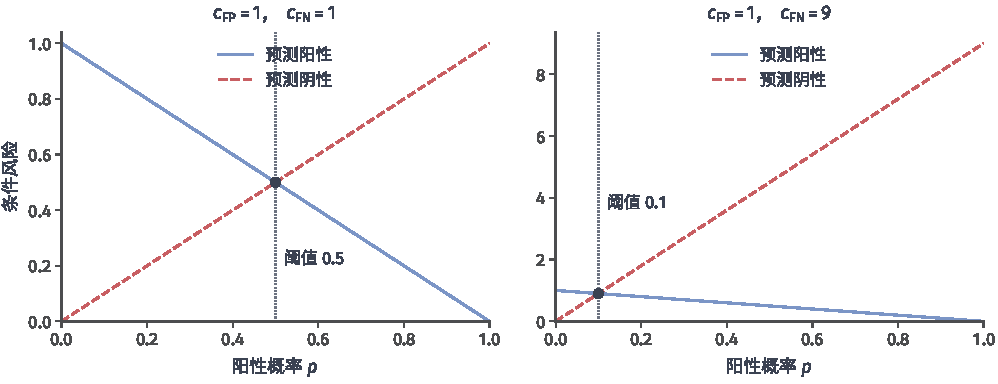
\includegraphics[width=\linewidth]{figures/01-mathematical-preliminaries/05-dynamical-systems-control-decision-and-games/matplotlib/decision-cost-thresholds/figure.pdf}
  \caption{二分类的条件风险。蓝色实线是预测阳性的$c_{\mathrm{FP}}(1-p)$，
  红色虚线是预测阴性的$c_{\mathrm{FN}}p$。左图两种错误成本均为$1$，阈值$0.5$；
  右图漏诊成本增至$9$，阈值降为$0.1$。横轴相同，纵轴分别显示各自损失范围。}
  \label{fig:decision-cost-thresholds}
\end{figure*}

允许拒答时，行动集合又发生改变。令类别为$\{1,\ldots,K\}$，分类采用零一损失，
增加拒答行动$\bot$，其成本为$c_{\mathrm R}\in(0,1)$。
最可能类别的条件错误风险为$1-p_{\max}(x)$，其中
$p_{\max}(x)=\max_k\mathbb P(Y=k\mid X=x)$。与拒答成本比较得
\begin{equation}
  \delta^\star(x)=
  \begin{cases}
    \argmax_k\mathbb P(Y=k\mid X=x),&p_{\max}(x)\geq1-c_{\mathrm R},\\
    \bot,&p_{\max}(x)<1-c_{\mathrm R}.
  \end{cases}
  \label{eq:decision-reject-rule}
\end{equation}
类别并列仍按固定次序选择。拒答是有自身代价的行动，不是结果分布中的新类别。
定义\term{覆盖率}（coverage）和正覆盖率下的接受风险
\[
  \operatorname{Coverage}(\delta)=\mathbb P\{\delta(X)\neq\bot\},\qquad
  R_{\mathrm{acc}}(\delta)
  =\mathbb E[\ell(\delta(X),Y)\mid\delta(X)\neq\bot].
\]
这里的覆盖率是接受行动的输入比例；第~\ref{sec:probability-exchangeability-conformal-ranks}节
预测集合的覆盖率$\mathbb P\{Y\in C(X)\}$则衡量集合包含真实响应的概率。
两者使用同一名称，但判断的事件不同。
多拒绝样本可以降低接受风险，所以必须同时报告覆盖率。
固定拒答成本最小化的是包含拒答损失的总体风险，不等于任意指定覆盖率下的
接受风险最小化。

人工复核预算会耦合不同观测点。若要求覆盖率至少为$\kappa$，问题为
\[
  \min_\delta R(\delta)
  \quad\text{s.t.}\quad\mathbb P\{\delta(X)\neq\bot\}\geq\kappa.
\]
在适当条件下，拉格朗日乘子可以把覆盖预算换成拒答的影子价格，仍产生阈值规则，
但阈值由整体分布和预算决定。\term{选择性预测}（selective prediction）选择在哪些
输入上行动，不等同于增大某类错误的代价。

\begin{example}[覆盖预算耦合两个观测点]
\label{ex:decision-two-point-coverage-budget}
设$X$等概率取$x_1,x_2$，两处最优分类错误风险为$0.2,0.4$，拒答损失均为$0.1$。
逐点无约束规则会全部拒答，覆盖率为零。要求覆盖率至少$1/2$且使用确定规则时，
至少接受一个点。接受$x_1$、拒答$x_2$的总体风险为
$\tfrac12\times0.2+\tfrac12\times0.1=0.15$；反向安排为
$\tfrac12\times0.1+\tfrac12\times0.4=0.25$；全部接受为$0.3$。
因此应把有限接受量安排在$x_1$。预算使两个观测点不能再独立执行原拒答规则。
\end{example}

若观测和行动有限，并允许按每个观测的行动概率优化，风险与覆盖约束都是线性的，
得到线性规划，强对偶提供影子价格。只允许确定规则时，选择变量带零一约束，
一般成为整数规划，不能套用普通LP强对偶。连续分布或非凸策略类还要检查可行性、
闭性与约束资格，不能仅写出乘子就宣称不存在对偶间隙。

最后核对随机化本身的作用。给定$x$，按概率核$q(\mathrm da\mid x)$选行动的风险为
\[
  \int_{\mathcal A}r(a\mid x)q(\mathrm da\mid x)\geq\inf_a r(a\mid x).
\]
有限或可数行动时就是加权和。没有额外耦合约束，随机化不能优于最佳纯行动；
最小值达到时，只有将概率放在最优行动上才保持最优。总体预算、公平或资源约束下，
随机化可实现确定规则达不到的平均比例，其作用来自可行域，不是期望损失偏好掷硬币。

\subsection{离散演化下的策略优化}
\label{sec:decision-dynamic-programming}

\subsubsection{有限时域下的最优策略递推}

多步任务中，行动的“损失表”要把后续机会也计入。先计算最后一步可以达到的最小成本，
再用它评价前一步行动，就得到
\begin{align}
  V_H^\star(s)&=c_H(s),
  \label{eq:decision-finite-bellman-terminal}\\
  V_t^\star(s)&=\min_{a\in\mathcal A(s)}
    \left\{c_t(s,a)+\sum_{s'}P_t(s'\mid s,a)V_{t+1}^\star(s')\right\}.
  \label{eq:decision-finite-bellman}
\end{align}
与固定评价式~\eqref{eq:decision-policy-bellman}相比，这里才出现行动最小化；
被最小化的是当前成本与继续价值之和，不只是当前成本。

图~\ref{fig:bellman-evaluation-versus-optimization}将固定策略评价与最优递推并列：两边都先对随机后继价值取期望，再分别按策略平均或在行动之间取最小值。

\begin{figure*}[htbp]
  \centering
  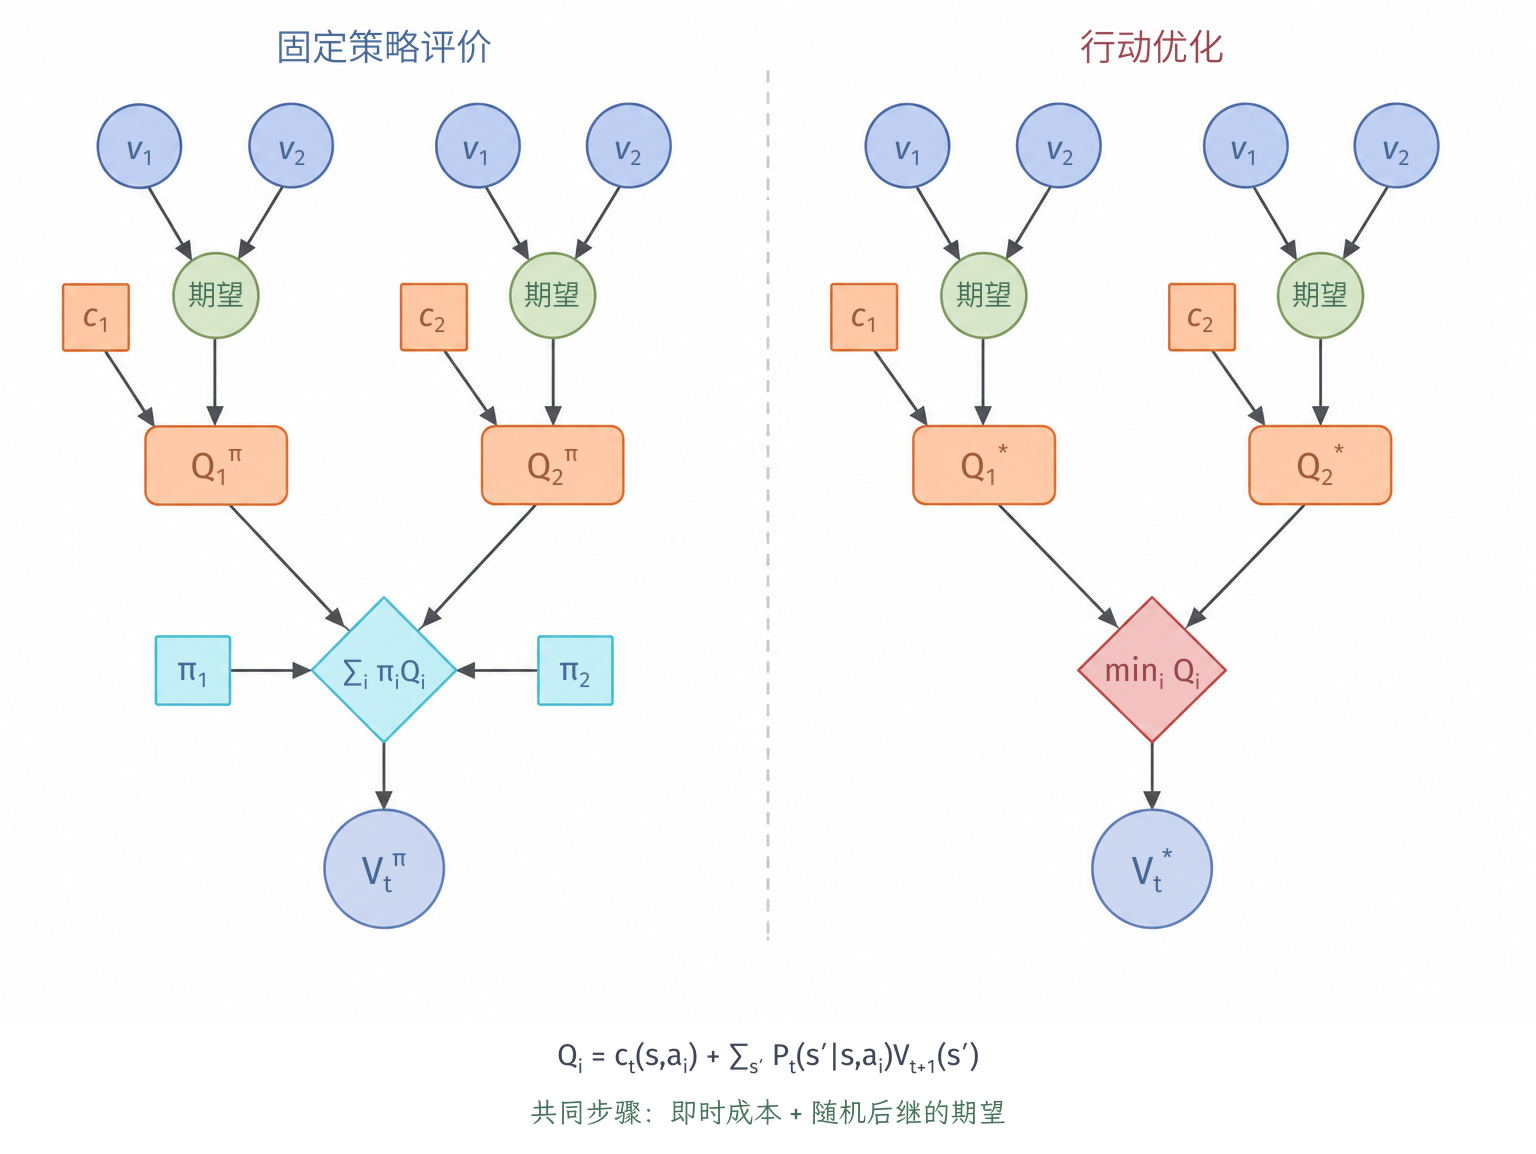
\includegraphics[width=\linewidth]{figures/01-mathematical-preliminaries/05-dynamical-systems-control-decision-and-games/generated/bellman-evaluation-versus-optimization/figure.png}
  \caption{成本口径下的两种Bellman递推。两边都先将即时成本与随机后继价值的期望相加；
  固定策略评价再按$\pi_t(a\mid s)$平均，最优递推则在允许行动之间取最小值，
  不能把行动最小化移到随机后继状态上。图中$c_i=c_t(s,a_i)$、$\pi_i=\pi_t(a_i\mid s)$；
  $v_1,v_2$是下一时刻两个后继状态的价值，左侧使用$V_{t+1}^\pi$，右侧使用$V_{t+1}^\star$，
  不暗示两边数值相同。有限时域边界为$V_H=c_H$，此处没有折扣系数。}
  \label{fig:bellman-evaluation-versus-optimization}
\end{figure*}


\begin{theorem}[有限时域最优性原理]
\label{thm:decision-finite-horizon-optimality}
在定义~\ref{def:decision-finite-mdp-policy}的有限MDP中，对每个末状态为$s$的历史
$h_t$，上述递推满足
$V_t^\star(s)=\inf_\pi J_t^\pi(h_t)$，其中下确界遍历全部允许的历史依赖随机继续策略。
各时刻各状态选择一个达到最小值的行动，构成达到该值的确定性Markov策略。
\end{theorem}
\begin{proof}
用逆向归纳。时刻$H$没有行动，终端成本就是最小继续成本。
假设每段末状态为$s'$的历史$h_{t+1}$的最小继续成本均为$V_{t+1}^\star(s')$。
固定末状态为$s$的$h_t$，任意策略先按$\pi_t(a\mid h_t)$选行动。
给定$a,s'$后，归纳假设说明其后续条件期望至少为$V_{t+1}^\star(s')$。
Markov转移保证下一状态分布是$P_t(\cdot\mid s,a)$，所以
\[
  J_t^\pi(h_t)\geq
  \sum_a\pi_t(a\mid h_t)
    \left[c_t(s,a)+\sum_{s'}P_t(s'\mid s,a)V_{t+1}^\star(s')\right]
  \geq V_t^\star(s).
\]
最后一步是有限个行动后果的凸组合不小于最小项。
反向在当前选择一个最小行动，并在每个下一状态采用归纳构造的最优Markov策略，
所有不等式均取等号。有限行动保证每次最小值达到，逆推到起点即得结论。
\end{proof}
证明比较了所有历史随机策略，不只比较Markov策略。Markov策略足够，是因为当前状态
概括了转移和期望累计目标所需信息；遗漏状态、整段轨迹的非加性指标或跨历史预算
都可能破坏这个前提。

\begin{example}[两阶段路线选择]
\label{ex:decision-two-stage-route}
回到前面固定的路线分布。终端价值就是终端损失，当前成本均为零，因而
\[
  Q_0(s_0,\text{稳妥})=2,\qquad
  Q_0(s_0,\text{捷径})=0.8\times0+0.2\times6=1.2.
\]
这里$Q_0$表示先指定当前行动、以后最优时的成本。期望准则应选择捷径，
而固定随机策略的成本$2-0.8p$也在$p=1$达到最小。
没有声称捷径每次都更好；它有概率$0.2$产生比稳妥更高的损失。
\end{example}

表~\ref{tab:decision-route-risk-criteria}保留同一轨迹模型，但改换评价口径。
风险偏好属于任务设定，不能在算完期望最优后将它解释成任意意义下的“最稳妥”。
\begin{table}[htbp]
  \centering
  \begin{tabular}{lcc}
    \toprule
    损失评价 & 稳妥 & 捷径\\
    \midrule
    $\mathbb E[L]$ & $2$ & $1.2$\\
    $P(L>3)$ & $0$ & $0.2$\\
    $\operatorname{VaR}_{0.9}(L)$ & $2$ & $6$\\
    $\operatorname{CVaR}_{0.9}(L)$ & $2$ & $6$\\
    \bottomrule
  \end{tabular}
  \caption{固定路线分布下的不同评价。捷径最坏$10\%$完全位于损失$6$的原子中，
  所以此处VaR与CVaR相同；这不是一般恒等式。增加违规概率预算后需重新选择策略。}
  \label{tab:decision-route-risk-criteria}
\end{table}

\subsubsection{无限折扣时域下的最优策略计算}

保留有限状态行动、时不变转移、有界成本及$0\leq\gamma<1$。与给定策略的
$T^\pi$不同，Bellman最优算子为
\begin{equation}
  (TV)(s)=\min_{a\in\mathcal A(s)}
    \left\{c(s,a)+\gamma\sum_{s'}P(s'\mid s,a)V(s')\right\}.
  \label{eq:decision-discounted-bellman-operator}
\end{equation}
对有限实数族$(u_a),(v_a)$，
$|\min_a u_a-\min_a v_a|\leq\max_a|u_a-v_a|$。
结合转移概率的非负性与归一化，得到
\begin{align}
  |(TV)(s)-(TW)(s)|
  &\leq\gamma\max_a
    \left|\sum_{s'}P(s'\mid s,a)(V(s')-W(s'))\right|\notag\\
  &\leq\gamma\lVert V-W\rVert_\infty,
  \label{eq:decision-bellman-contraction-pointwise}\\
  \lVert TV-TW\rVert_\infty&\leq\gamma\lVert V-W\rVert_\infty.
  \label{eq:decision-bellman-contraction}
\end{align}
有限维最大范数空间完备，定理~\ref{thm:analysis-banach-fixed-point}给出唯一固定点
$V^\star$。价值迭代$V^{(k+1)}=TV^{(k)}$从任意初值出发满足
\begin{equation}
  \lVert V^{(k)}-V^\star\rVert_\infty
  \leq\gamma^k\lVert V^{(0)}-V^\star\rVert_\infty.
  \label{eq:decision-value-iteration-error}
\end{equation}
固定点评价与最优性仍是两件事，必须证明该点由策略达到，并且不大于所有其他策略价值。

在每个状态选一个使$TV^\star(s)$取到最小值的行动，得到平稳确定策略$\pi^\star$。
此时$T^{\pi^\star}V^\star=TV^\star=V^\star$。固定策略评价算子的唯一固定点是
$V^{\pi^\star}$，由唯一性得$V^{\pi^\star}=V^\star$，所以候选值可实现。

再对任意历史依赖随机策略$\pi$比较。固定点满足每个状态行动的不等式
\[
  V^\star(s)\leq c(s,a)+\gamma\sum_{s'}P(s'\mid s,a)V^\star(s').
\]
沿策略实际选择的行动条件化，再把下一步的不等式代入，重复$n$步得到
\begin{equation}
  V^\star(s)\leq\mathbb E_s^\pi
  \left[\sum_{t=0}^{n-1}\gamma^tc(S_t,A_t)+\gamma^nV^\star(S_n)\right].
  \label{eq:decision-discounted-all-policy-comparison}
\end{equation}
该操作不要求$\pi$平稳，因为每一历史选择的行动都满足同一Bellman不等式。
余项绝对值至多$\gamma^n\lVert V^\star\rVert_\infty$，趋于零；
有界成本保证折扣级数可积。令$n\to\infty$得到$V^\star(s)\leq V^\pi(s)$。
与可达到性合起来，$\pi^\star$对全部允许历史随机策略最优。

若$\gamma=1$，严格压缩和尾项消失不再自动成立。长期平均成本
\[
  \limsup_{T\to\infty}\frac1T
    \mathbb E^\pi\left[\sum_{t=0}^{T-1}c(S_t,A_t)\right]
\]
采用了不同的目标：它衡量长期每步的成本，不是令折扣系数为$1$后直接累加全部成本。
要用同一个标量描述各初态的长期最优平均，需控制策略诱导链的常返结构。
有限模型的一种常见假设是：每项平稳确定性策略诱导的链都只有一个封闭常返类，
允许其余状态在进入该类之前被访问。这称为单链（unichain）假设；
它不要求只有一个状态，也不要求所有策略产生同一个转移矩阵。
在有限状态行动的单链模型中，平均成本最优性方程可写为
\[
  g+h(s)=\min_a\left\{c(s,a)+\sum_{s'}P(s'\mid s,a)h(s')\right\}.
\]
其中$g$是最优的长期每步平均成本，相对价值（relative value）$h(s)$记录从不同状态出发时，
相对于这个平均基线的成本偏移。对达到右侧最小值的平稳策略，逐步求和给出
\[
 \mathbb E_s\sum_{t=0}^{n-1}c(S_t,A_t)
 =ng+h(s)-\mathbb E_s h(S_n).
\]
这说明$ng$负责随时间增长的主项，$h$负责起点与终点的修正；有限状态下有界的修正除以$n$后消失。
方程的存在性属于平均成本理论，不能由前面的折扣压缩证明直接推出\scite{math-puterman1994mdp}

例如没有行动选择，两状态$s_0,s_1$确定性交替，阶段成本分别为$0,2$。
长期平均为$g=1$；取$h(s_0)=0,h(s_1)=1$，两状态的方程分别为
$1=0+1$与$2=2+0$。无折扣累计成本随时间发散，$h$却只记录状态之间的有限偏移。
给$h$加任意常数仍满足同一方程，可以约定参考状态$h(s_{\mathrm{ref}})=0$
消除这一自由度；这不等于已有折扣固定点的唯一性证明仍然适用。

连续状态或行动中，还需可测转移、适当的成本下半连续性、非空可行动作及紧致性或
强制性条件，再用可测选择将点态最小行动拼成策略。部分观测时只能使用允许信息；
信念状态只有在充分概括历史时才能承担这一角色。形式上写出$\inf$不等于它可达到。

\subsubsection{基于价值界与占用流量的最优性验证}

Bellman不等式给出一个有用的验证办法：提出一组状态价值下界，检查它对所有行动都成立。
与其对偶的是策略访问各状态行动对的折扣频率。给定初始分布$\mu_0$，价值端LP为
\begin{equation}
  \begin{aligned}
    \max_V\quad &(1-\gamma)\sum_s\mu_0(s)V(s)\\
    \text{s.t.}\quad&
      V(s)\leq c(s,a)+\gamma\sum_{s'}P(s'\mid s,a)V(s'),
      \quad s\in\mathcal S,\ a\in\mathcal A(s).
  \end{aligned}
  \label{eq:decision-value-lp}
\end{equation}
任意可行$V$满足$V\leq TV$，算子单调使
$V\leq TV\leq T^2V\leq\cdots$。令迭代收敛得到$V\leq V^\star$；
$V^\star$自身可行，因而达到最优值。
若$\mu_0$不在所有状态上为正，LP最优解未必唯一，但逐状态最大的可行向量仍是$V^\star$。

为每条不等式引入$d(s,a)\geq0$。最大化原问题的拉格朗日函数为
\[
  \begin{aligned}
    \mathcal L(V,d)&=(1-\gamma)\sum_s\mu_0(s)V(s)\\
    &\quad-\sum_{s,a}d(s,a)
      \left[V(s)-c(s,a)-\gamma\sum_{s'}P(s'\mid s,a)V(s')\right].
  \end{aligned}
\]
由于$V$自由取实值，$\sup_V\mathcal L(V,d)$有限当且仅当每个$V(s)$的系数为零，
即
\begin{equation}
  \sum_a d(s,a)=(1-\gamma)\mu_0(s)
    +\gamma\sum_{\bar s,\bar a}
      P(s\mid\bar s,\bar a)d(\bar s,\bar a).
  \label{eq:decision-discounted-flow-conservation}
\end{equation}
余下常数项为$\sum_{s,a}d(s,a)c(s,a)$，得到对偶
\begin{equation}
  \begin{aligned}
    \min_d\quad&\sum_{s,a}d(s,a)c(s,a)\\
    \text{s.t.}\quad&
      \text{式~\eqref{eq:decision-discounted-flow-conservation}},\qquad d(s,a)\geq0.
  \end{aligned}
  \label{eq:decision-occupancy-lp}
\end{equation}
原LP可行且有有限最优值，对偶也由下述任一策略产生可行点，
故有限LP强对偶定理~\ref{thm:opt-lp-strong-duality}给出两端最优值相等。

\begin{definition}[归一化折扣占用度量]
\label{def:decision-discounted-occupancy}
给定初始分布$\mu_0$、$0\leq\gamma<1$和允许策略$\pi$，归一化折扣
\term{占用度量}（occupancy measure）为
\begin{equation}
  d_\pi(s,a)=(1-\gamma)\mathbb E_{S_0\sim\mu_0}^\pi
    \left[\sum_{t=0}^\infty\gamma^t
      \mathbb I\{S_t=s,A_t=a\}\right].
  \label{eq:decision-discounted-occupancy}
\end{equation}
\end{definition}
它把同一状态行动在不同时刻的访问概率折扣相加，总质量为$1$，
通常不是Markov链的平稳分布。一般历史策略也有这样的占用。
分离$t=0$并将剩余时间索引前移，得到
\begin{align*}
  \sum_a d_\pi(s,a)
  &=(1-\gamma)\sum_{t=0}^\infty\gamma^t\mathbb P^\pi(S_t=s)\\
  &=(1-\gamma)\mu_0(s)
    +\gamma(1-\gamma)\sum_{t=0}^\infty\gamma^t
      \sum_{\bar s,\bar a}
      \mathbb P^\pi(S_t=\bar s,A_t=\bar a)P(s\mid\bar s,\bar a)\\
  &=(1-\gamma)\mu_0(s)+\gamma\sum_{\bar s,\bar a}
      P(s\mid\bar s,\bar a)d_\pi(\bar s,\bar a).
\end{align*}
所以流量方程的两项正是起点注入和后续转移注入。对状态求和得
$\sum_{s,a}d_\pi(s,a)=(1-\gamma)+\gamma\sum_{s,a}d_\pi(s,a)$，
从而总质量为$1$。成本对应关系为
\begin{equation}
  \sum_{s,a}d_\pi(s,a)c(s,a)
  =(1-\gamma)\mathbb E_{S_0\sim\mu_0}^\pi
    \left[\sum_{t=0}^\infty\gamma^tc(S_t,A_t)\right].
  \label{eq:decision-occupancy-cost}
\end{equation}

反过来，任一可行非负流量$d$也能实现。令$x_d(s)=\sum_a d(s,a)$，
在$x_d(s)>0$处定义$\pi_d(a\mid s)=d(s,a)/x_d(s)$，
零占用状态任意选行动。记相应转移矩阵为$\bm P_{\pi_d}$，状态占用列向量为$\bm x_d$，
则流量方程为
\[
  \bm x_d=(1-\gamma)\bm\mu_0+\gamma\bm P_{\pi_d}^{\top}\bm x_d.
\]
$\bm P_{\pi_d}$为行随机矩阵，$\bm I-\gamma\bm P_{\pi_d}^{\top}$的Neumann级数收敛，
因为$\lVert\gamma\bm P_{\pi_d}^{\top}\rVert_1=\gamma<1$。
所以此方程唯一可解。实际执行$\pi_d$所产生的状态占用满足同一方程，
必等于$\bm x_d$；再乘$\pi_d(a\mid s)$即恢复原来的$d(s,a)$。
因此对偶变量不是虚构的频率，而是可实施平稳随机策略的真实折扣访问分布。

互补松弛给出
\[
  d^\star(s,a)>0\ \Longrightarrow\
  V^\star(s)=c(s,a)+\gamma\sum_{s'}P(s'\mid s,a)V^\star(s').
\]
最优访问中实际使用的行动必须达到Bellman最小值。若不乘归一化因子$1-\gamma$，
流量方程起点项应为$\mu_0$，总质量为$1/(1-\gamma)$，目标也须同步改变。
连续状态下，占用成为测度、价值约束成为函数不等式；可测选择、紧致性和闭性等条件
仍需另证，不能只将求和改成积分便宣称强对偶成立。

\subsubsection{线性二次成本下的有限时域策略}

有限MDP通过逐行动枚举求最小值，线性二次模型则能利用代数结构直接求出最小行动。
前章定义~\ref{def:control-finite-horizon-lqr}已经给出有限时域LQR的问题，
定理~\ref{thm:control-finite-horizon-lqr}完整建立了Riccati递推及最优反馈。
本节只把这个结果接到本章的策略价值接口，不重复定义或配方证明。

该模型的最优继续价值具有
$V_t^\star(\bm x)=\bm x^\top\bm P_t\bm x+\beta_t$的形式。
式~\eqref{eq:control-lqr-bellman}是本节Bellman原理在连续线性状态上的具体版本：
线性动态代入下一步二次价值，仍得到关于当前状态和行动的二次函数；
前章通过严格正定的行动二次项求得
式~\eqref{eq:control-lqr-gain}的反馈增益，并由
式~\eqref{eq:control-discrete-riccati-recursion}反向计算$\bm P_t$。
零均值独立加性噪声的影响计入
式~\eqref{eq:control-lqr-noise-constant}的价值常数，不应在计算期望成本时丢弃。

给定反馈的评价只需代入该反馈；求最优反馈才需要对二次行动项最小化。
有限时域的最优性来自剩余成本的完整比较，不能推出无限时域闭环稳定；
后者使用前章定理~\ref{thm:control-infinite-horizon-lqr}的稳定化条件。
共同温度例的总输入成本也提醒我们，换成偏移输入$(u-0.4)^2$会改变目标。
若使用偏差坐标，应将原成本中的常数项和一次项一并变换，不能只套一个零目标LQR公式。

\subsection{连续演化下的策略优化}
\label{sec:control-hjb}

连续时间仍使用“当前一段成本加剩余最优价值”的原理，只是这一段可以任意短。
缩短时间间隔后，确定性速度产生价值的一阶导数，扩散噪声留下二阶导数。
方程给出局部关系，验证定理再把它与整段轨迹的最优性连接起来。

\subsubsection{确定性轨迹的价值方程}

考虑从$(\bm x,t)$出发的受控系统与成本
\begin{align}
  \dot{\bm x}(s)&=\bm f(\bm x(s),\bm u(s),s),\qquad \bm x(t)=\bm x,
  \label{eq:control-continuous-dynamics}\\
  J_{t,\bm x}(\bm u)
  &=\phi(\bm x(T))+\int_t^T\ell(\bm x(s),\bm u(s),s)\,\mathrm ds.
  \label{eq:control-continuous-cost}
\end{align}
状态属于$\mathbb R^n$，动作属于非空集合$U$。允许控制须可测、满足动作及状态约束，
并使轨迹在所考察时段存在、成本有限；反馈还须可由已有信息实现。
例如局部Lipschitz动态和适当增长界可用于保证常微分方程的适定性，
但写出一个不连续反馈后仍需重新核验。定义最优价值
$V(\bm x,t)=\inf_{\bm u}J_{t,\bm x}(\bm u)$。

若控制类对截断和前后拼接封闭，且具有所需近似最优选择，动态规划关系为
\begin{equation}
  V(\bm x,t)=\inf_{\bm u|_{[t,t+\Delta]}}
  \left\{\int_t^{t+\Delta}\ell(\bm x(s),\bm u(s),s)\,\mathrm ds
    +V(\bm x(t+\Delta),t+\Delta)\right\}.
  \label{eq:control-continuous-dpp}
\end{equation}
理由分为两边：任意全程控制的后半段成本不小于到达状态的最优继续价值，
所以全程下确界不小于右侧；反之将近似最优的短段与到达状态的近似最优继续控制拼接，
再使误差趋零，给出反向不等式。一般状态空间必须保证这些继续选择可测，
不能只对每条路径分别宣称存在一个后续控制。

经典方程的推导另假设$V\in C^1$、动态规划成立，且$\bm f,\ell$的连续性使短时
轨迹偏移为$O(\Delta)$。对参与逼近的控制还要求下面余项局部一致；
紧致动作集与相应局部有界连续系数是常见的充分条件。
以下在无状态约束的空间或约束不活跃的内部推导，保证所用常值动作在足够短的区间可行；
约束边界需另配边界条件。先用任意常值动作$\bm u$，
\begin{align*}
  V(\bm x(t+\Delta),t+\Delta)
  &=V(\bm x,t)+\Delta\,\partial_tV(\bm x,t)\\
  &\quad+\Delta\,\nabla_{\bm x}V(\bm x,t)^\top\bm f(\bm x,\bm u,t)
    +o(\Delta),\\
  \int_t^{t+\Delta}\ell(\bm x(s),\bm u,s)\,\mathrm ds
  &=\Delta\,\ell(\bm x,\bm u,t)+o(\Delta).
\end{align*}
用该控制代入下确界，只能先得到
\[
  -\partial_tV(\bm x,t)
  \leq\ell(\bm x,\bm u,t)+\nabla_{\bm x}V(\bm x,t)^\top\bm f(\bm x,\bm u,t).
\]
它对所有$\bm u\in U$成立，所以左侧不超过右侧的动作下确界。
要得到等式，还需要另一个方向，而不能把“任意动作”直接改写成“最优动作”。

固定$\eta>0$，取短段目标距下确界不超过$\eta\Delta$的允许控制。
沿轨迹使用链式法则，短段成本与价值增量等于
$\int_t^{t+\Delta}(\ell+\partial_sV+\nabla V^\top\bm f)\,\mathrm ds$。
一致余项允许把状态与时间冻结在$(\bm x,t)$；每个瞬时动作的Hamilton量均不低于
其动作下确界，于是
\[
  \partial_tV(\bm x,t)+
  \inf_{\bm u\in U}\{\ell(\bm x,\bm u,t)+
    \nabla_{\bm x}V(\bm x,t)^\top\bm f(\bm x,\bm u,t)\}
  \leq\eta+o(1).
\]
先令$\Delta\downarrow0$、再令$\eta\downarrow0$，与前一方向合并得到
\term{Hamilton--Jacobi--Bellman方程}（HJB）：
\begin{equation}
  -\partial_tV(\bm x,t)=
  \inf_{\bm u\in U}
    \{\ell(\bm x,\bm u,t)+
      \nabla_{\bm x}V(\bm x,t)^\top\bm f(\bm x,\bm u,t)\},
  \qquad V(\bm x,T)=\phi(\bm x).
  \label{eq:control-deterministic-hjb}
\end{equation}
花括号中的Hamilton量把瞬时成本和沿当前速度的价值变化率相加，
不是动力系统中沿轨迹守恒的Hamilton能量函数。
成本最小化对应这里的$\inf$和$-\partial_tV$；收益最大化须同步改换符号
\scite{math-bardi1997hjb}

\begin{theorem}[确定性HJB验证定理]
\label{thm:control-hjb-verification}
设候选$V\in C^1$满足式~\eqref{eq:control-deterministic-hjb}及终端条件。
假设每个允许控制都产生存在到$T$的轨迹，沿轨迹的链式法则和成本积分成立。
若有可实现反馈$\bm u^\star=\kappa(\bm x,t)$逐点达到HJB下确界，
且闭环轨迹存在到$T$并满足所有可行条件，则$V$为最优价值，$\kappa$为最优反馈。
\end{theorem}
\begin{proof}
任取允许控制，HJB的下确界不大于代入该动作的值，所以沿轨迹
\[
  \partial_sV(\bm x(s),s)+
  \nabla_{\bm x}V(\bm x(s),s)^\top
    \bm f(\bm x(s),\bm u(s),s)
  +\ell(\bm x(s),\bm u(s),s)\geq0.
\]
前两项由链式法则合为$\mathrm dV(\bm x(s),s)/\mathrm ds$。
从$t$积分到$T$，用终端条件得到$J_{t,\bm x}(\bm u)\geq V(\bm x,t)$。
因而候选值是所有允许成本的共同下界。
对$\kappa$，逐点达到下确界使不等式处处取等号，
积分后$J_{t,\bm x}(\kappa)=V(\bm x,t)$，所以它达到共同下界，完成验证。
\end{proof}
HJB是光滑最优价值满足的局部关系；验证定理则把一个候选解变成全程最优性的证书。
只在若干采样点降低方程残差还不够，还需终端或边界条件、极小动作的可实现性、
轨迹存在性及整个相关区域上的方程关系。

\subsubsection{随机轨迹的价值方程}

随机轨迹无法逐条预先选择，但可以优化允许策略的期望成本。设$\bm W_s$为
$d$维标准Brownian运动，状态满足
\begin{equation}
  \mathrm d\bm X_s=\bm f(\bm X_s,\bm u_s,s)\,\mathrm ds
    +\bm\Sigma(\bm X_s,\bm u_s,s)\,\mathrm d\bm W_s,
  \label{eq:control-stochastic-dynamics}
\end{equation}
其中$\bm\Sigma$为$n\times d$矩阵。允许控制对给定滤过渐进可测，
不得使用未来Brownian增量，并满足解存在、约束与成本可积的要求。
价值为
$\inf_{\bm u}\mathbb E_{t,\bm x}[
\phi(\bm X_T)+\int_t^T\ell(\bm X_s,\bm u_s,s)\,\mathrm ds]$；
下标表示从$(t,\bm x)$重启过程，避免对零概率初态事件直接作比值条件化。

对$V\in C^{2,1}$应用第~\ref{chap:dynamical-systems-and-state-estimation}章的
Itô公式，固定动作的受控生成元为
\[
  \mathcal L^{\bm u}V=
  \nabla_{\bm x}V^\top\bm f+
  \frac12\operatorname{tr}
    (\bm\Sigma\bm\Sigma^\top\nabla_{\bm x}^2V).
\]
随机积分在可积鞅条件下的条件均值为零，二次变差却留下了二阶项。
在动态规划、近似最优选择及局部一致的短时展开条件下，先代入常值动作得到一个方向，
再沿$\eta\Delta$-最优控制积分并令$\Delta,\eta$趋零，得到
\begin{equation}
  \begin{aligned}
  -\partial_tV(\bm x,t)=\inf_{\bm u\in U}\biggl\{&
    \ell(\bm x,\bm u,t)+
    \nabla_{\bm x}V(\bm x,t)^\top\bm f(\bm x,\bm u,t)\\
    &+\frac12\operatorname{tr}\!\left[
      \bm\Sigma(\bm x,\bm u,t)\bm\Sigma(\bm x,\bm u,t)^\top
      \nabla_{\bm x}^2V(\bm x,t)\right]\biggr\}.
  \end{aligned}
  \label{eq:control-stochastic-hjb}
\end{equation}
终端条件仍为$V(\bm x,T)=\phi(\bm x)$。这里对随机微分方程仅取均值后代入
确定性HJB，会遗漏扩散项。

\begin{theorem}[随机HJB验证]
\label{thm:control-stochastic-hjb-verification}
设$V$对状态二次、对时间一次连续可微，满足
式~\eqref{eq:control-stochastic-hjb}及终端条件。
假设每个允许控制都使受控过程存在到$T$，成本与Itô公式中的有限变差项可积，
且$\int_t^s\nabla_{\bm x}V^\top\bm\Sigma\,\mathrm d\bm W$为真鞅。
若可容许反馈$\bm u^\star=\kappa(\bm x,t)$逐点达到HJB下确界，
则$V$等于最优期望成本，$\kappa$达到该值。
\end{theorem}
\begin{proof}
对任意允许控制，HJB给出
$\partial_sV+\mathcal L^{\bm u_s}V+\ell(\bm X_s,\bm u_s,s)\geq0$。
沿轨迹应用Itô公式、积分并取从$(t,\bm x)$出发的期望，随机积分因真鞅条件消失，
得到
\[
  \mathbb E_{t,\bm x}\left[
    \phi(\bm X_T)+\int_t^T\ell(\bm X_s,\bm u_s,s)\,\mathrm ds\right]
  \geq V(\bm x,t).
\]
对$\kappa$，生成元不等式取等号，同一计算证明其期望成本等于共同下界$V$。
这验证的是期望最优，不是每条噪声实现上的路径最优。
\end{proof}

一个常用的充分鞅条件是
$\mathbb E\int_t^T\lVert\bm\Sigma^\top\nabla_{\bm x}V\rVert^2\,\mathrm ds<\infty$。
若只能得到局部鞅，应先在退出有界区域等停时$\tau_n$处停止，再证明成本积分、
$V(\bm X_{T\wedge\tau_n},T\wedge\tau_n)$等量能合法取极限，例如使用增长界、
矩估计与一致可积性。局部鞅不自动具有零期望，省略这一步会使验证结论失去依据。

若扩散矩阵与状态、动作都无关，二次价值的二阶项只增加状态无关的常数，
对应离散式~\eqref{eq:control-lqr-noise-constant}的现象。
若扩散依赖动作，它直接参与动作最小化；依赖状态时也可能改变价值形状。
因此噪声均值为零并不足以保证反馈不变。

\subsubsection{线性二次成本下的连续策略}

在线性动态$\dot{\bm x}=\bm A\bm x+\bm B\bm u$下，
取$\bm u\in\mathbb R^m$，阶段成本
$\ell(\bm x,\bm u)=\bm x^\top\bm Q\bm x+\bm u^\top\bm R\bm u$，
终端成本$\phi(\bm x)=\bm x^\top\bm Q_T\bm x$，其中
$\bm Q,\bm Q_T\succeq\bm0$、$\bm R\succ\bm0$。有限时域取平方可积控制，
固定有限矩阵保证线性轨迹存在。试取对称二次候选
\[
  V(\bm x,t)=\bm x^\top\bm P(t)\bm x,\qquad \bm P(T)=\bm Q_T.
\]
它是否确为价值要由HJB和验证定理确认，而不是由二次外形决定。
有
$\partial_tV=\bm x^\top\dot{\bm P}\bm x$、
$\nabla_{\bm x}V=2\bm P\bm x$。代入HJB后动作相关项为
$\bm u^\top\bm R\bm u+2\bm x^\top\bm P\bm B\bm u$，配方得
\begin{align*}
  \bm u^\top\bm R\bm u+2\bm x^\top\bm P\bm B\bm u
  ={}&
  (\bm u+\bm R^{-1}\bm B^\top\bm P\bm x)^\top
    \bm R(\bm u+\bm R^{-1}\bm B^\top\bm P\bm x)\\
  &-\bm x^\top\bm P\bm B\bm R^{-1}\bm B^\top\bm P\bm x.
\end{align*}
正定$\bm R$使第一项非负且仅在一个动作处为零，因此反馈为
\begin{equation}
  \bm u^\star(t)=-\bm R^{-1}\bm B^\top\bm P(t)\bm x(t).
  \label{eq:control-continuous-lqr-gain}
\end{equation}
把最小项代回，对所有$\bm x$比较二次型系数，得到
\begin{equation}
  -\dot{\bm P}
  =\bm Q+\bm A^\top\bm P+\bm P\bm A
    -\bm P\bm B\bm R^{-1}\bm B^\top\bm P,\qquad
  \bm P(T)=\bm Q_T.
  \label{eq:control-continuous-riccati}
\end{equation}
这是微分Riccati方程；价值边界给在终点，故从$T$向较早时刻反向积分。

有限时域上这些条件也保证不会在中途丢失所需解。矩阵常微分方程先在终端附近有唯一
局部对称解；在其存在区间，反馈连续，验证定理说明其二次型为非负最优成本，
并不大于零控制的有限成本。零控制在整个有限区间给出统一的二次上界，
于是$\bm0\preceq\bm P(t)\preceq M\bm I$，某个有限$M$适用于该区间。
局部Lipschitz的Riccati向量场因解有界而可继续延伸，直到起点。
因此该候选及反馈确实定义在整个有限时域。

还可以直接给出成本差证书。用Riccati方程化简沿任意允许轨迹的价值导数，得到
\[
  \ell(\bm x,\bm u)+\frac{\mathrm d}{\mathrm dt}
    [\bm x^\top\bm P(t)\bm x]
  =
  (\bm u+\bm R^{-1}\bm B^\top\bm P\bm x)^\top
    \bm R(\bm u+\bm R^{-1}\bm B^\top\bm P\bm x).
\]
积分后，任意策略的成本等于初始二次价值加右侧非负积分；
反馈使积分为零，最优性由此可以逐项核算。
例如$\dot x=u$、$Q=R=1,Q_T=0$时，
$P(t)=\tanh(T-t)$满足$-\dot P=1-P^2$，
反馈$u=-\tanh(T-t)x$，价值为$\tanh(T-t)x^2$。
越接近没有终端惩罚的截止时刻，控制增益越小，这也说明有限时域策略一般依赖时间。

无限时域的代数方程与稳定化条件由前章式~\eqref{eq:control-care}给出，
这里不把令$\dot{\bm P}=0$当作稳定性证明。
连续闭环需要特征值实部为负，离散闭环需要特征值位于单位圆内；
CARE与DARE分别服务于这两个问题，不能混用。

\subsubsection{非光滑与受限信息下的价值方程}

最优动作切换时，价值可能连续但没有处处存在的梯度。
经典HJB在折点不能直接代入，这不表示轨迹成本没有定义。
\term{黏性解}（viscosity solution）用光滑函数从上方或下方接触价值，
在接触点检验方程不等式；导数取自测试函数，价值本身可以不可微。

将确定性HJB写成
\[
  F(\bm x,t,a,\bm p)
  :=-a-\inf_{\bm u\in U}
      \{\ell(\bm x,\bm u,t)+\bm p^\top\bm f(\bm x,\bm u,t)\}=0,
\]
其中$a$代表时间导数，$\bm p$代表状态梯度。
\begin{definition}[连续价值函数的黏性解]
\label{def:control-viscosity-solution}
设$V$在方程作用域内连续。对任意光滑测试函数$\varphi$，
若$V-\varphi$在内点$(\bm x,t)$取局部最大值时均有
$F(\bm x,t,\partial_t\varphi,\nabla_{\bm x}\varphi)\leq0$，
称$V$为黏性次解。若局部最小值处均有相应的$F\geq0$，称为黏性上解。
同时满足两项，并按当前问题满足终端或边界条件的$V$称为黏性解。
\end{definition}
可将测试函数平移常数使接触时$V=\varphi$。
局部最大对应$\varphi$从上方接触，局部最小对应从下方接触；
不是任取一个斜率代入。随机二阶方程还需代入测试函数的Hessian。
光滑$V$取$\varphi=V$即恢复经典等式。适当的比较原理可由次解不高于上解推出唯一性，
但其方程结构、连续性、增长与边界条件仍需另证，定义本身不保证唯一或易于计算。

先看目标边界上的非光滑。令$\dot x=u,|u|\leq1$，每单位时间成本为$1$，
到达$\{0\}$即终止，则最短到达时间$V(x)=|x|$。在延续域$x\neq0$上，
\[
  0=1+\inf_{|u|\leq1}V'(x)u=1-|V'(x)|.
\]
正侧取$u=-1$、负侧取$u=1$，均推向原点。$x=0$是退出边界，
只需施加$V(0)=0$，不属于方程内部。这个例子不能单独证明内点必须使用黏性解；
要展示内点折角，需要一个不在原点提前退出的问题。

\begin{example}[延续域内部的价值折点]
\label{ex:control-viscosity-interior-kink}
仍取$\dot x=u,|u|\leq1$，改为固定终点$T$、零运行成本和终端成本$|x(T)|$。
剩余时间最多移动$T-t$，故
\[
  V(x,t)=\max\{|x|-(T-t),0\},\qquad
  -V_t+|V_x|=0,\qquad V(x,T)=|x|.
\]
内侧$|x|<T-t$可以到达原点并停留，价值为零；外侧只能减少$T-t$的距离。
折点$x=\pm(T-t)$位于$t<T$的延续域内部。例如$T-t=1$时，
$|x|\leq1$可完全纠正，$x=1.5$仍剩终端代价$0.5$。

正侧折点附近$V=\max\{x+t-T,0\}$。从下方接触的光滑函数的导数对
$(\varphi_x,\varphi_t)$为$(p,p)$、$0\leq p\leq1$，
即两侧斜率的凸组合，故$-\varphi_t+|\varphi_x|=-p+p=0$，满足上解条件。
向上折角不存在光滑上方接触函数，次解检验在该点无额外约束；
光滑区域满足经典等式。负侧接触导数为$(-p,p)$，同样满足等式。
这说明黏性条件能处理方程内部的切换折点，而不把切换面误当作退出边界。
\end{example}

有状态约束时，价值只在可行控制存在的区域定义。不可穿越边界需配合可行方向
或状态约束边界条件；允许触边退出则需退出成本。内部方程相同不能代替边界含义。
真实状态不可见时，也不能直接以$\bm x$作为反馈输入，一般须使用观测历史给出的
\term{信念状态}，通常是无限维分布。线性高斯二次模型的有限维分离是特殊结构，
将在下一节证明其成本最优性。

HJB比较累计成本，前章的屏障约束限定安全行动。将屏障二次规划用于修正一个性能反馈，
通常会改变原成本最优性；在HJB中直接加入约束则是另一个受约束优化问题。
稳定性证明使用的Lyapunov函数、最优价值和屏障函数分别服务于收敛、最优与不变性，
不能仅因它们都考察沿轨迹的标量变化而互换。

\subsection{受限信息下的策略选择}
\label{sec:decision-value-of-information}

\subsubsection{新增观测下的决策收益}

前面的最优规则都受到已有信息限制。如果先获得一次观测，后面的行动可能随观测改变，
这项改进能否抵偿获取成本？答案依赖任务损失，不只依赖观测减少了多少不确定性。
设未知环境参数为$\Theta$、当前信息为$\mathcal G$，信念为
$b(\mathrm d\theta)=\mathbb P(\Theta\in\mathrm d\theta\mid\mathcal G)$。
先取有限行动与可测可积损失；立即行动的最小风险为
\[
  \mathcal R(b)=\inf_a\mathbb E_{\theta\sim b}[\ell(a,\theta)].
\]
现在可先从给定核$K(\mathrm dz\mid\theta)$观察信号$Z$，得到后验$b_Z$，
再选适合该后验的行动。

\begin{definition}[期望样本信息价值]
\label{def:decision-expected-sample-information-value}
在上述有限行动、可积损失和信号核条件下，\term{期望样本信息价值}
（expected value of sample information, EVSI）为
\begin{equation}
  \operatorname{EVSI}(Z\mid b)
  =\mathcal R(b)-\mathbb E_{Z\mid b}[\mathcal R(b_Z)].
  \label{eq:decision-evsi}
\end{equation}
\end{definition}
观察后的$\inf_a$在对$Z$求期望之内：先见信号、再行动。
若把$\inf_a$放在外面，就强迫所有信号结果使用同一行动，丢失信息的用途。
这比较的是两种信息条件下的最优值，不是同一固定策略多观测一次后的数值变化。

EVSI非负，因为看到信号后总可忽略它。若原最优行动为$a^\star$，则
\[
  \mathcal R(b_z)\leq
  \mathbb E[\ell(a^\star,\Theta)\mid Z=z,\mathcal G].
\]
对$Z$平均并用塔式法则，得到
$\mathbb E_{Z\mid b}[\mathcal R(b_Z)]\leq
\mathbb E[\ell(a^\star,\Theta)\mid\mathcal G]=\mathcal R(b)$。
一般行动空间若下确界不达到，可用风险至多$\mathcal R(b)+\varepsilon$的行动，
作同样比较后令$\varepsilon\downarrow0$；但观察后的选择还须具有可测的
最优或近似最优规则。免费信息不降低最优收益，不意味着有成本的信息都值得购买：
获取成本为$k$时，净价值是$\operatorname{EVSI}-k$。

若直接知道$\Theta$，\term{完全信息价值}为
\begin{equation}
  \operatorname{EVPI}(b)
  =\inf_a\mathbb E_b[\ell(a,\Theta)]
    -\mathbb E_b[\inf_a\ell(a,\Theta)].
  \label{eq:decision-evpi}
\end{equation}
已知$\Theta$可模拟信号核，再执行任何基于信号的规则，
故$0\leq\operatorname{EVSI}\leq\operatorname{EVPI}$。
等号$\operatorname{EVSI}=\operatorname{EVPI}$表示信号已保留实现该任务最优行动所需的
信息，不要求重建参数的每个细节。

\begin{example}[辨别信号与无关信号]
\label{ex:decision-informative-and-irrelevant-signals}
阳性概率为$0.3$，假阳性损失为$1$、假阴性为$9$。
不取新信号时，两行动风险为$0.7$和$2.7$，所以$\mathcal R(b)=0.7$。
免费信号$Z_{\mathrm{perf}}$若完全揭示类别，观察后总能选对，
风险为零，EVSI为$0.7$。独立于类别的公平硬币$Z_{\mathrm{coin}}$不改变后验、
行动或风险，EVSI为零。若完全信号成本为$0.8$，其净价值为$-0.1$。
信息能否辨别类别、是否改善任务、是否抵偿获取成本，是三个不同判断。
\end{example}

互信息衡量关于$\Theta$的不确定性平均减少多少，EVSI衡量给定损失下最优决策改善多少。
信号可能精确揭示与行动无关的参数，互信息大而EVSI为零；另一个信号只在决策阈值附近
改变信念，却可能避免高代价行动。对数评分下，若行动本身是预测分布，最优期望对数损失
与条件熵对应，才得到信息增益与风险改善的直接联系。一般分类、分配和控制损失没有这种
自动等价；使用熵作为查询代理，需要额外论证它与任务成本的关系。

\subsubsection{未知收益下的探索价值}

信息不一定来自独立购买的信号，也可能来自行动自身的结果。
考虑两轮选择，每次成功奖励$1$、失败奖励$0$，本小节改用收益最大化，
对应成本为奖励的负值。已知臂的成功概率为$0.6$；
未知臂有一个两轮不变的参数$\Theta\in\{0.3,0.9\}$，先验各为$1/2$。
给定$\Theta$，各次奖励条件独立，已知臂结果不提供$\Theta$的信息。
每轮只看到所选臂结果，不看到未选臂的反事实结果。

两臂当前平均成功率均为$0.6$，只比第一轮即时收益会并列。
先选未知臂时，成功的边缘概率为$0.6$。看到成功后，
\[
  \mathbb P(\Theta=0.9\mid\text{成功})
  =\frac{0.9\times0.5}{0.9\times0.5+0.3\times0.5}=0.75,
\]
未知臂下一轮成功率为$0.75\times0.9+0.25\times0.3=0.75$，应继续选它。
若看到失败，
\[
  \mathbb P(\Theta=0.9\mid\text{失败})
  =\frac{0.1\times0.5}{0.1\times0.5+0.7\times0.5}=0.125,
\]
未知臂后验成功率为$0.125\times0.9+0.875\times0.3=0.375$，
下一轮应改选已知臂。因此两轮最优适应行动的期望收益为
\begin{equation}
  0.6+0.6\times0.75+0.4\times0.6=1.29.
  \label{eq:decision-two-arm-information-value}
\end{equation}
先选已知臂不会更新信念，第二轮仍并列，两轮收益为$1.2$。
多出的$0.09$来自第一轮观测改善第二轮选择，不来自未知臂的当前均值较高。

这就是\term{探索}（exploration）的决策作用：行动同时影响当前收益和未来信息。
只剩一轮时，信息没有使用机会，两臂又并列；试验成本、先验或剩余时域改变，
探索价值也会改变。若每轮同时看到所有臂，或$\Theta$随时间漂移，上述信息结构已不成立，
后验和$1.29$的计算也不再适用。一般多臂和强化学习算法还须处理长期规划、
未知参数与计算复杂度，这个两轮例子只定位信息价值从哪里进入策略。

自适应查询也改变统计证据的条件。因为过去观察决定下一次试验或停止时间，
不能把选中样本无条件视为固定设计下的独立同分布数据。
报告置信区间或最优行动识别保证时，应回用
第~\ref{sec:stoch-martingales-stopping-sequential-concentration}节的停时条件与
第~\ref{sec:stoch-self-normalized-adaptive-design}节的可预测设计，
检查行动是否在当前噪声揭晓前选定，以及误差保证是否对全部查看时刻同时成立。

遗憾使用另一个比较对象。令$Y_t$为第$t$轮奖励，
$\mathcal H_{t-1}$为行动前信息，行动$A_t$在$Y_t$揭晓前选定，
并假设对固定环境参数$\theta$，
\[
  \mathbb E[Y_t\mid\mathcal H_{t-1},A_t=a,\Theta=\theta]
  =\mu(a,\theta)\quad\text{几乎处处}.
\]
这里平均奖励不随轮次改变；条件均值假设使自适应选择后当前噪声仍正确中心化，
却不使访问次数或全部数据变成非自适应。令
$a^\star(\theta)\in\argmax_a\mu(a,\theta)$，累计伪遗憾为
\[
  \operatorname{Reg}_T(\theta)
  =\sum_{t=1}^T[\mu(a^\star(\theta),\theta)-\mu(A_t,\theta)].
\]
它比较同一环境下的平均奖励，而不是两条实现奖励轨迹之差。
算法和参数随机时还可再取期望；直接用实现奖励定义的遗憾含有奖励噪声。
一次信号的EVSI与长期伪遗憾相关，但前者不能替代后者的统计与序贯证明。

\subsubsection{线性高斯条件下的估计与行动分离}

一般情况下，行动改变未来信息，会像探索例那样同时影响估计和控制。
一个重要的例外是标准有限时域线性二次高斯控制（LQG）。
取
\[
  \bm x_{t+1}=\bm A\bm x_t+\bm B\bm u_t+\bm w_{t+1},
  \qquad \bm y_t=\bm C\bm x_t+\bm v_t,
\]
其中$\bm x_0$高斯，$\bm w_{t+1}\sim\mathcal N(\bm0,\bm W_t)$、
$\bm v_t\sim\mathcal N(\bm0,\bm N_t)$，$\bm W_t\succeq\bm0$、$\bm N_t\succ\bm0$，
初态与所有噪声相互独立，噪声跨时独立，协方差已知且不依赖控制。
先观察$\bm y_t$再行动，信息为
$\mathcal I_t=\sigma(\bm y_0,\bm u_0,\ldots,\bm u_{t-1},\bm y_t)$。
允许无输入或状态约束、具有有限二阶矩的$\mathcal I_t$-可测控制；
若使用私有随机数，也将独立于系统噪声的已用随机数计入可用信息。
目标为前章有限LQR的期望二次成本，状态和终端权重半正定、输入权重正定。

第~\ref{sec:dynamical-kalman-rts}节的有限时域Kalman递推给出
$\widehat{\bm x}_t=\mathbb E[\bm x_t\mid\mathcal I_t]$和更新后误差协方差
$\bm E_t=\mathbb E[(\bm x_t-\widehat{\bm x}_t)
(\bm x_t-\widehat{\bm x}_t)^\top\mid\mathcal I_t]$。
令$\bm e_t=\bm x_t-\widehat{\bm x}_t$，投影性质说明
$\mathbb E[\bm e_t\mid\mathcal I_t]=\bm0$，从而
\[
  \mathbb E[\bm x_t^\top\bm Q_t\bm x_t\mid\mathcal I_t]
  =\widehat{\bm x}_t^\top\bm Q_t\widehat{\bm x}_t
    +\operatorname{tr}(\bm Q_t\bm E_t).
\]
交叉项的条件期望为零，因而无条件也有
$\mathbb E[\widehat{\bm x}_t^\top\bm Q_t\bm e_t]=0$。
标准模型的关键在于$\bm E_t$由Kalman协方差递推确定，不依赖观测值或所选控制。
控制在预测均值中作为已知平移被扣除，不改变下一次观测的误差协方差。

只看这一项分解还不能证明全程最优，需要把所有未来动作的影响合在一起。
令$\bm P_t,\bm K_t$取前章有限LQR递推的结果，
$\bm M_t=\bm R_t+\bm B^\top\bm P_{t+1}\bm B\succ\bm0$。
回用前章逐步配方并对时间求和，任一允许输出策略$\mu$满足
\begin{align*}
  J^\mu={}&
    \mathbb E[\bm x_0^\top\bm P_0\bm x_0]
    +\sum_{t=0}^{H-1}\operatorname{tr}(\bm P_{t+1}\bm W_t)\\
    &+\sum_{t=0}^{H-1}\mathbb E[
      (\bm u_t+\bm K_t\bm x_t)^\top
      \bm M_t(\bm u_t+\bm K_t\bm x_t)].
\end{align*}
此式来自状态价值项的望远镜消去和独立零均值噪声的迹项，
不是假设输出策略已经最优。再对$\mathcal I_t$条件化，最后一项逐步分为
\begin{align*}
  &\mathbb E[
    (\bm u_t+\bm K_t\bm x_t)^\top\bm M_t
    (\bm u_t+\bm K_t\bm x_t)\mid\mathcal I_t]\\
  &\quad=
    (\bm u_t+\bm K_t\widehat{\bm x}_t)^\top\bm M_t
    (\bm u_t+\bm K_t\widehat{\bm x}_t)
    +\operatorname{tr}(\bm K_t^\top\bm M_t\bm K_t\bm E_t).
\end{align*}
所有迹项与初态项都不依赖策略。剩余各项非负，而可实施策略
\begin{equation}
  \bm u_t^\star=-\bm K_t\widehat{\bm x}_t
  \label{eq:policy-finite-lqg-feedback}
\end{equation}
使这些项同时为零，因而在全部允许输出策略中达到最小期望成本。
误差协方差产生的成本并未消失，只是不能通过该模型中的控制改变。

这就是\term{分离原则}：有限Kalman滤波按估计误差构造条件均值，
LQR增益按行动成本构造，再将二者连接。它比确定性观测器的谱分离多给出成本最优性，
却不要求有限时域滤波已经达到稳态；稳态滤波和输出反馈的稳定条件仍由前章负责。
受控观测、动作相关噪声、风险敏感目标、输入或状态约束会改变上述分解或可行性，
不能直接沿用这一结论。温度例中的有界两点噪声也不是这里的高斯假设；
若采用LQG模型，应显式另取独立高斯噪声，并放弃将有界安全区间视为逐路径必然保证。

\subsection{风险约束下的策略优化}
\label{sec:policy-risk-optimization}

现在把风险评价接口中的指定动作改成待选择动作。必须先固定目标：
嵌套条件风险可以按其定义逐步优化；静态总损失CVaR使用累计状态；
概率约束和候选模型又分别规定可行策略与最坏机制。它们并不是互换风险符号的同一个算法。

对有限状态行动、确定Markov策略和具有充分状态信息的嵌套风险，
单调性允许把每个下一状态的最优继续值用于当前比较：
\begin{align}
  V_H(s)&=c_H(s),\notag\\
  V_t(s)&=\min_{a\in\mathcal A(s)}
    \{c_t(s,a)+\rho_{t,s,a}(V_{t+1}(S_{t+1}))\}.
  \label{eq:decision-risk-bellman-finite}
\end{align}
有限时域的证明仍是逆向归纳，但将期望的保序性换成风险映射的单调性。
任一允许的历史依赖确定策略，其后续风险逐节点不低于$V_{t+1}$，
当前风险便不低于相应动作项；
取最小动作再接上各节点的最优继续策略达到此界。
这要求允许规则能逐历史拼接、风险模型在相同状态使用相同映射。
取条件期望恢复普通Bellman；取条件CVaR得到嵌套CVaR，而非静态CVaR
\scite{math-ruszczynski2010risk}

若允许随机行动并采用第~\ref{sec:policy-nested-risk-evaluation}节“先评价环境风险、
再平均行动风险”的口径，行动概率的目标为各动作项的线性组合，确定最小动作仍足够。
若声明风险作用于行动和下一状态的联合损失，则应优化概率分布$q\in\Delta(\mathcal A(s))$：
\[
  \inf_q\,\rho^q_{t,s}\bigl(c_t(s,A)+V_{t+1}(S')\bigr).
\]
不能无条件用期望的线性性把它写成动作风险的平均，再声称确定策略最优。
给定更具体的风险泛函可另证随机化是否有益；本节上式
~\eqref{eq:decision-risk-bellman-finite}的策略范围以已声明的口径为准。

无限折扣版本明确按“后续风险值再乘折扣”的目标定义算子
\begin{equation}
  (T_\rho V)(s)=\min_a
    \{c(s,a)+\gamma\rho_{s,a}(V(S'))\}.
  \label{eq:decision-risk-bellman-operator}
\end{equation}
成本有界、每个映射归一化、单调且平移等变时，
第~\ref{sec:policy-nested-risk-evaluation}节已证一步风险非扩张；
再用最小值差不等式得到
\begin{equation}
  \lVert T_\rho V-T_\rho W\rVert_\infty
  \leq\gamma\lVert V-W\rVert_\infty.
  \label{eq:decision-risk-bellman-contraction}
\end{equation}
因此$\gamma<1$时唯一固定点存在，价值迭代误差不超过
$\gamma^k\lVert V^{(0)}-V^\star_\rho\rVert_\infty$，
残差界为$\lVert T_\rho V-V\rVert_\infty/(1-\gamma)$。

最优解释还须补全。固定点的贪心策略使固定策略风险算子取同一个固定点，故达到该值。
有限截断问题用上述逆向归纳比较全部允许历史策略；若$|c|\leq C$，
归一化和非扩张使第$n$步以后的折扣风险影响至多为
$\gamma^nC/(1-\gamma)$，统一趋于零。因此截断最优值和各允许策略的截断值
可取极限，得到固定点不大于任何策略的无限嵌套风险。
如果原风险目标并非如此递归、状态遗漏历史信息或策略类不可拼接，
算子即使压缩，也只是稳定地计算另一个问题。

相干映射的包络把动作项改写成
\[
  c(s,a)+\gamma\sup_{q\in\mathcal Q(s,a)}
    \sum_{s'}q(s'\mid s,a)V(s').
\]
将它解释为逐时鲁棒最优，必须使用定义~\ref{def:decision-rectangular-uncertainty}
的矩形候选机制。共享未知参数的非矩形集合不能逐节点自由取最坏；
有限凸风险若有对偶罚项，也不能在优化时删去。

静态CVaR则回用第~\ref{sec:policy-static-cvar-evaluation}节的累计状态。
固定$\eta$，将式~\eqref{eq:policy-static-cvar-augmented-evaluation}中的行动概率汇总
改成行动最小化，得到
\[
  \begin{aligned}
    W_t^\eta(s,b)&=\min_a\sum_{s'}P_t(s'\mid s,a)
      W_{t+1}^\eta(s',b+\gamma^tc_t(s,a)),\\
    W_H^\eta(s,b)&=(b+\gamma^Hc_H(s)-\eta)_+.
  \end{aligned}
\]
随后计算
\[
  \inf_\pi\operatorname{CVaR}_\alpha(L^\pi)
  =\inf_{\eta\in\mathbb R}
    \left\{\eta+\frac{1}{1-\alpha}
      \sum_s\mu_0(s)W_0^\eta(s,0)\right\}.
\]
两层均为下确界，因此交换$\inf_\pi,\inf_\eta$不需要极小极大定理，
但须说明策略类：这里允许时间、物理状态和累计成本上的策略，
并假设可测选择与所需达到性。阈值是起点选定的常数，不能到未来看到损失后重新挑选。
若原问题只允许不读取累计成本的策略，这项动态规划可能扩大可行策略类；
若只存在下确界，可使用近似最优阈值和策略，不能宣称必有最优解。

概率约束问题例如
$\inf_{\pi:\,\mathbb P^\pi(E)\leq\varepsilon}\mathbb E^\pi[L]$
限制的是特定违规事件$E$。终端、逐时和全程事件须分别定义；
全程约束可能需要增广累计违规标记或剩余风险预算。
路线例要求$\mathbb P^\pi(L>3)\leq0.1$时，随机策略须满足$0.2p\leq0.1$，
即$p\leq1/2$。期望损失$2-0.8p$在$p=1/2$取$1.6$；
若只允许确定行动，则只有稳妥可行，成本$2$。随机化的作用来自概率约束的可行比例，
不能用无约束纯策略最优结论排除它。

最坏模型目标为
\[
  \inf_{\pi\in\Pi_{\mathrm{adm}}}
    \sup_{Q\in\mathcal P}\mathbb E_Q^\pi[L].
\]
单步时退化为$\inf_a\sup_Q\mathbb E_Q[\ell(a,Y)]$，参数模型用$Q=P_\theta$。
$\Pi_{\mathrm{adm}}$须规定信息和约束，$\mathcal P$须规定模型能否随历史改变。
对偶、极小极大交换和局部递推分别有自己的条件。
评价准则、时间一致性、可行性与计算收敛各回答一项问题，不能用其中一个替代其他检查。

\section{本章小结}
\label{sec:decision-theory-and-dynamic-risk-summary}

同一两阶段路线任务串起了本章四个步骤。策略先规定走捷径的概率$p$，
再与环境共同产生概率为$1-p,0.8p,0.2p$的三条轨迹；给每条轨迹计价后，
期望损失为$2-0.8p$，尾部指标和违规概率还描述它的其他后果。
固定$p$计算这些量是评价，允许改变$p$才是优化。期望准则选$p=1$，
概率预算可能要求$p\leq1/2$，因此“最优”离不开准则和可行域。

平均收益、一次实现收益和尾部损失不是同一个对象。VaR给出分位阈值，
CVaR平均最坏尾部，并在分位原子上按需要补足概率质量。
风险包络重加权既定分布，模型不确定集改变候选机制，机会约束限制违规事件。
逐时获得信息后，静态总损失CVaR可能发生条件偏好反转；
嵌套风险以单调递归保持时间一致性，却定义了不同目标。
固定策略的风险计算必须说明行动随机性是否也进入风险映射；
逐节点最坏模型还必须与矩形候选集合一致。

期望评价以指定策略的行动概率汇总，Bellman优化才把它换成行动最小值。
有限时域由逆向归纳证明最优性，有限折扣问题由压缩性、可达到性和全历史策略比较
共同完成证明。占用流量把价值下界与可实现访问频率连接起来。
连续时间则用HJB描述局部最优关系，并用终端条件、光滑性、轨迹可行性与可积条件
验证全程成本；非光滑内点和状态边界不能省略相应的解概念与边界要求。

新增信息只有通过改变后续行动才产生决策价值。EVSI比较观察前后的最优风险，
探索把即时收益和未来信息放在同一策略中；标准有限LQG的特殊结构才允许估计与行动
分开设计并保持期望成本最优。温度例同样显示，误差收敛后仍要比较舒适偏差与能耗成本，
且总输入计价不能偷换为偏移输入计价。

价值迭代收敛描述的是计算序列$V^{(k)}$，闭环状态收敛描述的是执行轨迹$x_t$，
二者不是同一个时间轴上的同一结论。稳定与安全条件回到前章核验；
后续多方策略问题还要研究其他参与者同时选择行动时的响应，以及策略更新序列如何演化。

\chapter{多方策略的响应与演化}
\label{chap:game-theory-and-multi-agent-decision}

两个人共用一个房间，却分别控制一台加热器。一人增加供热，不仅改变自己的舒适程度，
也改变另一人的温度和下一步选择。第~\ref{chap:control-theory}章研究给定反馈怎样
控制状态，第~\ref{chap:decision-theory-and-dynamic-risk}章在既定环境中比较策略价值；
现在环境中还有会选择、会调整的参与者。一个人算出的最优策略依赖对方，而对方也在
作同样的计算。怎样定义这种相互依赖的选择？双方都愿意维持的策略组合是否存在，
实际调整又是否会走到那里？

回答这些问题，须分开三种对象：一局内的行动与状态、给定信息下的完整策略、
多局学习形成的策略序列。先确定策略能够依赖什么信息，才能计算其价值和允许的偏离；
排除有利偏离得到均衡条件，给出更新规则才得到动态系统。即使策略持续变化，也可以
比较整个序列与一个固定替代策略的累计表现。温度模型用于区分这几层判断，匹配硬币
用于展示随机化与循环，三张牌质询博弈则保留私人信息、完整计划和局部学习之间的联系。
合作时还要另问共同收益怎样分配，以及成员是否愿意接受分配。

\section{策略的多方行动与信息}
\label{sec:game-actions-information}

\subsection{参与者与联合行动}
\label{sec:game-joint-actions}

只写一人的行动还不足以确定房间温度或对局结果，需要把同一时刻所有人的选择放在一起。
战略式博弈用参与者、可选行动和各自收益描述这种依赖；它是一张完整的比较规则，
尚未规定各人怎样找到行动。

% Baseline B:333-341
\begin{definition}[有限战略式博弈]
\label{def:game-finite-strategic-game}
有限\(n\)人\term{战略式博弈}（strategic-form game）由参与者集合
\(N=\{1,\ldots,n\}\)、每人的有限行动集\(A_i\)和收益函数
\[
  u_i:A_1\times\cdots\times A_n\to\mathbb{R}
\]
组成，各$A_i$均非空。
\end{definition}

联合行动记为\(\bm a=(a_1,\ldots,a_n)\in\prod_i A_i\)。双人有限行动时，可以把
各人的收益列成一张表，从而得到矩阵表示。
% Baseline B:23-35
\begin{definition}[有限矩阵博弈]
\label{def:game-finite-matrix-game}
有限双人\term{矩阵博弈}（matrix game）由两组非空有限行动
\(A_1=\{1,\ldots,m\}\)、\(A_2=\{1,\ldots,n\}\)和两张收益矩阵
\(\bm{U}_1,\bm{U}_2\in\mathbb{R}^{m\times n}\)给出。第1位参与者选择行，第2位
参与者选择列，落在\((i,j)\)时，两人的收益分别为
\(\bigl((\bm{U}_1)_{i,j},(\bm{U}_2)_{i,j}\bigr)\)。若存在矩阵\(\bm{M}\)使
\(\bm{U}_1=\bm{M}\)、\(\bm{U}_2=-\bm{M}\)，双方收益之和恒为零，就得到
\term{零和博弈}（zero-sum game）。
\end{definition}
一个人增加的收益正好是另一个人的损失，因此
零和情形只需记录第1位参与者的收益矩阵\(\bm{M}\)；一般和情形则不能省略第二张矩阵。

温度与能耗通常不满足零和关系。
以下温度扩展也使用联合行动，但行动连续，不属于刚才的有限博弈定理的适用范围。

\begin{example}[两方共同加热的状态与成本]
\label{ex:game-two-heaters}
沿用温差状态\(x_t\)，把原单方加热量明确扩为两个输入之和：
\begin{equation}
  x_{t+1}=0.8x_t+u_{1,t}+u_{2,t}+w_{t+1},
  \qquad y_t=x_t+v_t.
  \label{eq:game-two-heater-dynamics}
\end{equation}
本章计算先取\(w_{t+1}=v_t=0\)。每个局内时刻，双方先观察\(x_t=y_t\)，
再同时选择各自的\(u_{i,t}\)，两项输入共同推动下一状态；本次选择不预先看到
对方的本次行动。后面的交替响应描述跨轮策略更新，不改变这项局内信息约定。默认
\(u_{i,t}\in\mathbb R\)，这是允许正负调温的无约束教学模型；若只允许加热或增加安全
约束，必须重新求解约束响应。给定局内时域\(H\)，第\(i\)方的成本可写成
\[
  J_i(\pi_1,\pi_2;x_0)
  =\sum_{t=0}^{H-1}
  \bigl[(x_{t+1}-r_i)^2+\lambda_i u_{i,t}^2\bigr],
  \qquad \lambda_i>0,
\]
其中\(\pi_i\)把本人可用历史映射为行动，\(r_i\)是舒适目标，
\(\lambda_i\)是本人能源代价权重。用于最大化的收益为\(-J_i\)，不是\(J_i\)。
\end{example}

若双方目标同为\(2\)，维持\(x_t=2\)要求总输入为\(0.4\)，并非每人都输入
\(0.4\)。对固定反馈
\(u_{i,t}=a_i-k_i(x_t-2)\)，只有\(a_1+a_2=0.4\)时，误差才满足
\[
  x_{t+1}-2=(0.8-k_1-k_2)(x_t-2).
\]
因此总增益为\(0.3\)时才复现前章的误差系数\(0.5\)。这只是给定联合反馈后的状态
计算，不证明该反馈对任一方最优。两方反馈的选择及更新须另行分析。

\subsection{纯策略与混合策略}
\label{sec:game-pure-mixed}

在匹配硬币中，双方同时选正面\(H\)或反面\(T\)，相同则第1方得\(1\)，不同则得
\(-1\)，第2方收益相反。固定选择某一面会给对方留下针对它的机会，于是需要随机化：
用一个概率分布选择行动，而不是在一局里把两个行动各执行一半。
% Baseline B:37-52
\begin{definition}[纯策略与混合策略]
\label{def:game-pure-mixed-strategy}
直接选择某一行或某一列称为\term{纯策略}（pure strategy）。在行动上选择概率分布
称为\term{混合策略}（mixed strategy）。记
\[
  \Delta_m
  =
  \left\{
    \bm{x}\in\mathbb{R}^m:
    \bm{x}\geq\bm{0},\
    \bm{1}^{\top}\bm{x}=1
  \right\}
\]
为\(m\)个行动上的概率单纯形。双方以各自的混合策略独立抽取行动。
\end{definition}

对一般有限行动集写作\(\bm\sigma_i\in\Delta(A_i)\)，联合策略为
\(\bm\sigma=(\bm\sigma_1,\ldots,\bm\sigma_n)\)，其余人的策略组合记为
\(\bm\sigma_{-i}\)。这里“联合策略”是各人的规则集合；若各人独立抽样，联合行动
服从乘积分布。如果共同装置抽取一个行动组合，再私下向各人发建议，联合分布可以相关。
两种方式即便具有同样的边缘概率，也可能产生不同收益；具体计算见
第~\ref{sec:game-payoff-relations}节。

单纯形\(\Delta_m\)嵌在\(\mathbb R^m\)中，维数为\(m-1\)，顶点对应纯行动。
匹配硬币只需一个数\(p\in[0,1]\)表示第1方选\(H\)的概率，另一个数\(q\)表示
第2方的同类概率。此时的策略空间是正方形，而不是四个纯行动组合。

\subsection{行动历史与可用信息}
\label{sec:game-extensive-information}

矩阵中的一个“行动”有时其实是一整份计划。要判断计划能否执行，需要还原每一步
发生的时间与行动者所见的信息。
% Baseline B:122-128
考虑高牌\(H\)、中牌\(M\)和低牌\(L\)。庄家从\(H\)与\(L\)中等概率发给参与者1
一张隐藏牌，\(M\)留作公共比较基准。参与者1看到自己的牌后选择质询\(B\)或放弃
\(P\)。放弃时收益为\(0\)。质询后，参与者2只知道发生了质询，不知道隐藏牌，并选择
应对\(C\)或退让\(F\)。退让时参与者1得到\(1\)；应对时，高牌使参与者1得到\(2\)，
低牌使其得到\(-2\)。参与者2得到相反收益。

这就是本章的三张牌教学任务：只随机发出高、低牌，中牌是公开比较基准，并非第三种
可能的私有牌。质询和应对发生在同一局的不同节点；学习算法在下一局改变概率，是另一个
时间尺度。
% Baseline B:797-856
\begin{definition}[有限扩展式博弈的历史树]
\label{def:game-finite-extensive-history}
\term{扩展式博弈}（extensive-form game）用历史树保留这些信息。记\(H\)为非空有限历史
集合，空历史为\(\varnothing\)。它满足前缀封闭：若一串行动属于\(H\)，删去末尾
若干行动所得的前缀仍属于\(H\)。不能再延长的历史组成终止集合\(Z\subset H\)。
若\(h\notin Z\)，可选行动集合\(A(h)\)规定合法后继\(ha\)，参与者函数\(P(h)\)
指出下一步由哪位参与者行动；机会节点记为\(P(h)=c\)，其行动概率
\(\sigma_c(a\mid h)\)已给定、非负且在\(A(h)\)上和为\(1\)。终止历史\(z\)为每位
参与者给出收益\(u_i(z)\)。对各参与者，还需指定下面的信息集划分，才能完整确定博弈。
\end{definition}

三张牌质询博弈的机会节点先选择\(H\)或\(L\)，概率各为\(1/2\)。参与者1看到牌面，
所以“拿到\(H\)”与“拿到\(L\)”属于两个不同决策位置。若他选择\(P\)，历史立即
终止；若选择\(B\)，参与者2行动。参与者2只看到“发生了质询”，无法区分历史
\((H,B)\)与\((L,B)\)。

对参与者\(i\)，记全部由其行动的非终止历史为
\[
  H_i=\{h\in H\setminus Z:P(h)=i\}.
\]
\begin{definition}[信息集]
\label{def:game-information-set}
参与者\(i\)的\term{信息集}（information set）族\(\mathcal{I}_i\)是\(H_i\)
的一个划分，每个信息集\(I\in\mathcal{I}_i\)收集参与者当时无法区分的决策历史。
同一信息集中的历史必须具有相同的合法行动集，记这个共同集合为
\(A(I)=A(h)\)，其中\(h\in I\)。
\end{definition}
否则参与者连“现在能做什么”都无法由观察确定。
牌面例子中，参与者2的信息集为
\[
  I_2=\{(H,B),(L,B)\},
\]
可选行动都是\(\{C,F\}\)。信息集不是状态的另一名称。第
~\ref{sec:decision-dynamic-programming}节中的Markov状态用于预测给定行动后的未来
分布；信息集描述当前参与者无法区分哪些历史。两个节点可以有相同物理状态，却因参与者
记得不同过去而属于不同信息集，也可以物理状态不同却因观察受限而位于同一信息集。
参与者\(i\)的纯策略必须为每个\(I\in\mathcal{I}_i\)指定一个
\(A(I)\)中的行动，包括均衡路径上不会到达的信息集；因此它是一份完整的应急计划，
而不只是实际走过路径上的动作序列。

表~\ref{tab:game-card-information}将同一个小博弈中“真实发生了什么”和“行动者
能区分什么”并列写出。参与者2在两条质询历史上必须用同一个$c$，因为他看到的数据
相同。若直接为高牌和低牌分别设置$c_H,c_L$，便改变了可用信息，得到另一个博弈，
即使收益函数没有改动也不能复用当前的均衡。

\begin{table*}[htbp]
  \centering
  \begin{tabularx}{\linewidth}{lXXX}
    \toprule
    行动者 & 真实决策历史 & 当时可区分的信息 & 合法行动规则\\
    \midrule
    参与者1 & 拿到$H$或拿到$L$ & 私人牌面可见，属于两个信息集 & 可分别选$b_H,b_L$\\
    参与者2 & $(H,B)$或$(L,B)$ & 只看到质询，属于同一信息集 & 两条历史共用应对概率$c$\\
    机会 & 初始发牌 & 已给定的环境随机化 & $P(H)=P(L)=1/2$，参与者不能选择\\
    \bottomrule
  \end{tabularx}
  \caption{三张牌教学博弈的信息约束。$b_H,b_L$为对应牌面上的质询概率，$c$为
  参与者2看到质询后的应对概率。这些行为策略记号将在下一小节正式使用。}
  \label{tab:game-card-information}
\end{table*}

参与者2不能规定“高牌质询就应对，低牌质询就退让”，因为他无法区分这两个节点。
若公开牌面，信息集就拆成两个单点集合，可实施的策略集合已经改变；不能继续使用隐藏牌
博弈的解。对零概率历史，也须预先规定行动，才能比较完整策略偏离。
但Nash条件不唯一规定零概率信息集上的信念；讨论每处的序贯理性还需额外条件。

\subsection{完整策略与行为策略}
\label{sec:game-complete-behavior}

三张牌中，第1方的完整纯计划按“高牌时行动、低牌时行动”有
\((P,P),(B,P),(P,B),(B,B)\)四种，第2方有\(F,C\)两种。
开局随机抽一份完整计划是一种实现方式；另一种是在真正到达信息集时才抽行动，
称为行为策略，也就是把随机选择写在每个可辨认的决策位置上。
% Baseline B:860-871
\begin{definition}[行为策略]
\label{def:game-behavior-strategy}
参与者\(i\)的\term{行为策略}（behavior strategy）
\(\sigma_i(a\mid I)\)在每个信息集\(I\in\mathcal{I}_i\)上分别给出$A(I)$上的概率分布；
同一信息集中的所有历史必须使用同一分布。
\end{definition}
三张牌例子可写成三个数：
\[
  b_H=\sigma_1(B\mid I_H),\qquad
  b_L=\sigma_1(B\mid I_L),\qquad
  c=\sigma_2(C\mid I_2).
\]
% Baseline B:877-944
战略式中的混合策略是在游戏开始时随机抽取一个完整纯计划；行为策略则在每个信息集
到达时随机选择。二者在一般情形下并不等价。若参与者会忘记自己早先知道的牌或采取的
行动，开局抽取的同一个随机计划可以在多个时刻制造相关性，而独立的局部随机化未必能
复制这种相关性。

\begin{definition}[完全回忆]
\label{def:game-perfect-recall}
\term{完全回忆}（perfect recall）要求参与者在同一信息集内不能混淆自己过去获得的
信息和采取的行动。更具体地说，任意两个属于同一信息集的历史，沿途经过的该参与者
信息集序列及其本人行动序列必须相同；这里的过去序列只记录当前节点之前的本人决策。
\end{definition}

\begin{theorem}[Kuhn实现等价]
\label{thm:game-kuhn-equivalence}
在有限完全回忆扩展式博弈中，对任一参与者，任意混合策略都存在一个行为策略，使二者
面对任意固定的对手与机会策略时诱导相同的终止历史分布；任意行为策略也存在具有同样
性质的混合策略。
\end{theorem}

\begin{proof}
先从混合策略构造行为策略。设\(\mu_i\)是在有限纯策略集合上的分布。完全回忆保证
每个信息集\(I\)都有唯一的本人前缀
\[
  \rho_i(I)
  =
  \bigl((I_1,a_1),\ldots,(I_k,a_k)\bigr),
\]
即到达\(I\)以前本人依次经过的信息集和采取的行动；同一\(I\)中的所有历史共享这条
前缀。记\(E_I\)为纯策略与这条前缀一致的事件。若
\(\mu_i(E_I)>0\)，定义
\[
  \sigma_i(a\mid I)
  =
  \frac{
    \mu_i\bigl(E_I\cap\{s_i:s_i(I)=a\}\bigr)
  }{
    \mu_i(E_I)
  },
\]
其中\(s_i\)表示一项完整纯策略，事件\(s_i(I)=a\)表示它在当前信息集指定行动
\(a\)；若分母为零，
就在\(A(I)\)上任取一个分布。

沿任意终止历史依次考察参与者\(i\)的行动。链式法则表明，\(\mu_i\)抽取的完整计划
与这条本人行动序列一致的概率，等于上述各条件概率的乘积，也就是行为策略
\(\sigma_i\)沿该历史贡献的到达概率。对手与机会的路径概率在两种表示下相同，所以
每个终止历史的总概率相同。分母为零的信息集只位于\(\mu_i\)赋予零概率的本人前缀
之后，任意补全都不改变这一结论。

反过来，给定行为策略\(\sigma_i\)，在游戏开始前为每个信息集独立抽取一个行动，并
把全部抽取结果组成纯策略\(s_i\)。令
\[
  \mu_i(s_i)
  =
  \prod_{I\in\mathcal{I}_i}
  \sigma_i\bigl(s_i(I)\mid I\bigr).
\]
对任意终止历史，把未出现在该历史上的信息集行动求和后都得到因子\(1\)，剩余因子
恰是行为策略沿该历史的行动概率乘积。因此该混合策略面对任意对手与机会策略，也诱导
与原行为策略相同的终止历史分布。
\end{proof}

完全回忆不能省略。考虑一位参与者先在\(I_1\)选择\(L\)或\(R\)，随后到达同一个
信息集\(I_2\)，却忘记了刚才的选择，并在\(I_2\)选择\(l\)或\(r\)。混合策略可以
各以\(1/2\)抽取完整计划\((L,l)\)与\((R,r)\)，只产生\(Ll\)和\(Rr\)两条历史。
任何行为策略若让第一步的\(L,R\)都以正概率出现，且让第二步的\(l,r\)也都以正概率
出现，就还会以正概率产生\(Lr\)和\(Rl\)；若把某个概率设为零，又无法同时保留前两条
历史各\(1/2\)的概率。因此局部独立随机化不能复现混合计划中的跨时相关性。

牌面例满足完全回忆，因为每人只行动一次。比如以概率\(2/3\)抽取\((B,P)\)、
以概率\(1/3\)抽取\((B,B)\)，等价于\(b_H=1,b_L=1/3\)的行为策略；
此处只验证表示等价，其价值及最优性将在收益计算和响应条件中分别核对。
Kuhn定理等同的是面对任意固定对手时的终局分布，不是说两种随机装置内部完全相同。

\section{策略的多方价值}
\label{sec:game-multiparty-value}

策略已经给定时，计算的是这些规则实际产生什么收益，不需要猜测参与者以后怎样改进。
有限行动表按联合概率加权，历史树按终局概率加权，两者都使用各方自己的收益。
合作分配还需先定义联盟能共同取得的价值；这个额外模型不能从一人的收益自动推出。

\subsection{给定策略下的收益计算}
\label{sec:game-fixed-policy-payoffs}

\subsubsection{联合行动下的期望收益}
\label{sec:game-joint-expected-payoff}

各人独立随机化时，联合行动\(\bm a\)的概率为\(\prod_j\sigma_j(a_j)\)，所以
% Baseline B:349-358
\begin{equation}
  u_i(\bm{\sigma})
  =
  \sum_{\bm{a}\in A_1\times\cdots\times A_n}
  \left(
    \prod_{j=1}^{n}\sigma_j(a_j)
  \right)
  u_i(\bm{a}).
  \label{eq:game-mixed-payoff-extension}
\end{equation}
后文仍用\(u_i\)表示纯行动收益及其混合延拓，参数能区分二者。双人矩阵中，
\(u_i(\bm x,\bm y)=\bm x^\top\bm U_i\bm y\)；零和时只需记录行方的收益：
% Baseline B:55-60
\begin{equation}
  u(\bm{x},\bm{y})
  =
  \bm{x}^{\top}\bm{M}\bm{y}.
  \label{eq:game-matrix-expected-payoff}
\end{equation}

若改用相关联合分布\(\mu\)，应计算
\[
  u_i(\mu)=\sum_{\bm a}\mu(\bm a)u_i(\bm a),
\]
不能把\(\mu\)擅自换成边缘概率的乘积。

匹配硬币的行方收益矩阵为
\[
  \bm M_{\mathrm{mp}}=
  \begin{pmatrix}1&-1\\-1&1\end{pmatrix}.
\]
按四个联合行动的概率加权，得到混合收益
\[
  \begin{aligned}
    u_1(p,q)&=pq+(1-p)(1-q)\\
      &\quad-p(1-q)-(1-p)q\\
      &=(2p-1)(2q-1).
  \end{aligned}
\]
给定\(q\)，纯行动\(H,T\)的收益分别为\(2q-1,1-2q\)。
例如\(p=3/4,q=1/4\)时，第1方期望收益为\(-1/4\)，第2方为\(1/4\)；
双方均匀随机时，两人的期望收益都是\(0\)。这些数是给定策略的评价，
尚未检查任何人愿不愿意改变。

\subsubsection{行动历史下的整局价值}
\label{sec:game-history-value}

历史树中，一条终局路径可能包含多次行动。要算整局收益，先把沿途概率相乘，
再按各终局收益求和。这里的路径概率与条件续局概率即使在当前不会到达的节点，
也可由策略本身计算，不必对零概率事件作除法。
% Baseline B:953-971
给定联合行为策略\(\bm{\sigma}\)，历史
\[
  h=(a_1,\ldots,a_k)
\]
的\term{到达概率}（reach probability）是沿路径各次行动概率之积。把机会也看作
固定策略，可以写成
\begin{equation}
  \pi^{\bm{\sigma}}(h)
  =
  \pi_i^{\bm{\sigma}}(h)
  \pi_{-i}^{\bm{\sigma}}(h),
  \label{eq:game-reach-factorization}
\end{equation}
其中\(\pi_i^{\bm{\sigma}}(h)\)只乘参与者\(i\)在路径上的行动概率，
\(\pi_{-i}^{\bm{\sigma}}(h)\)则乘其他参与者与机会的概率。这个分解不会声称两部分
随机变量独立；它只是把同一条路径上的乘积按行动者归组。

从历史\(h\)继续到终止历史\(z\)的条件路径概率记为
\(\pi^{\bm{\sigma}}(h,z)\)。

更明确地，若\(h_t\)是第\(t\)步前的历史，机会贡献为
\(\pi_c(h)=\prod_{t:P(h_t)=c}\sigma_c(a_t\mid h_t)\)，本人贡献为
\(\pi_i^{\bm\sigma}(h)=\prod_{t:P(h_t)=i}\sigma_i(a_t\mid I(h_t))\)；
空积为\(1\)，而\(\pi_{-i}^{\bm\sigma}(h)=\pi_c(h)\prod_{j\ne i}\pi_j^{\bm\sigma}(h)\)。
因此整局价值为
\begin{equation}
  u_i(\bm\sigma)=\sum_{z\in Z}\pi^{\bm\sigma}(z)u_i(z).
  \label{eq:game-terminal-payoff}
\end{equation}
若收益由局内阶段收益累计而来，可先对每条路径求累计收益再取期望；这与
第~\ref{sec:decision-dynamic-programming}节的续局价值使用同一求和原则，
只是现在路径概率由多方共同决定。

三张牌的六类终局概率可以直接核对：
\[
\begin{array}{c@{\quad}c@{\quad}r}
 z&\pi^{\bm\sigma}(z)&u_1(z)\\ \hline
 (H,P)&(1-b_H)/2&0\\
 (L,P)&(1-b_L)/2&0\\
 (H,B,F)&b_H(1-c)/2&1\\
 (L,B,F)&b_L(1-c)/2&1\\
 (H,B,C)&b_Hc/2&2\\
 (L,B,C)&b_Lc/2&-2
\end{array}
\]
它们的概率之和为\(1\)，从而
\begin{equation}
  u_1(b_H,b_L,c)
  =\frac12 b_H(1+c)+\frac12 b_L(1-3c),
  \qquad u_2=-u_1.
  \label{eq:game-card-behavior-payoff}
\end{equation}
例如全部取\(1/2\)时，两项分别为\(3/8\)与\(-1/8\)，整局收益为\(1/4\)。
在\((b_H,b_L,c)=(1,1/3,1/3)\)下，整局收益为\(2/3\)，发生质询的概率为
\((b_H+b_L)/2=2/3\)。给定已经质询，Bayes公式给出高、低牌概率为\(3/4,1/4\)；
因此此条件下第2方应对或退让的收益均为\(-1\)。条件收益不是事前收益：
后者还需乘上质询概率，放弃路径则贡献零。

把第1方四个完整计划分别代入式~\eqref{eq:game-card-behavior-payoff}，
并按\(F,C\)排列列方行动，就得到同一个扩展式博弈的战略式收益矩阵：
% Baseline B:131-143
\begin{equation}
  \bm{M}
  =
  \begin{pmatrix}
    0 & 0\\
    1/2 & 1\\
    1/2 & -1\\
    1 & 0
  \end{pmatrix}.
  \label{eq:game-card-normal-form}
\end{equation}
例如，计划\((B,P)\)只在拿到高牌时质询。对方退让时，收益以一半概率为\(1\)、一半
概率为\(0\)，故矩阵元素为\(1/2\)；对方应对时，相应期望为\(1\)。

该矩阵已经对机会发牌取过期望，不能在后续矩阵运算中再乘一次\(1/2\)。
在信息集上比较局部学习信号时，还会有意去掉本人的到达概率；
第~\ref{sec:game-counterfactual-comparison}节将说明这为何不同于条件期望。

\subsection{对抗与共同收益的价值关系}
\label{sec:game-payoff-relations}

同一行动空间上可以有不同的利益关系。\term{一般和博弈}（general-sum game）
允许各人收益独立规定；共同收益模型则让所有人使用同一个收益函数。
下表固定双方行动\(L,R\)，只改变收益规则，各格均按第1方、第2方排列。
\begin{table*}[htbp]
  \centering
  \begin{tabularx}{\linewidth}{lXXXX}
    \toprule
    收益关系 & $(L,L)$ & $(L,R)$ & $(R,L)$ & $(R,R)$\\
    \midrule
    零和匹配 & $(1,-1)$ & $(-1,1)$ & $(-1,1)$ & $(1,-1)$\\
    一般和选择 & $(2,2)$ & $(0,3)$ & $(3,0)$ & $(1,1)$\\
    共同协调 & $(2,2)$ & $(0,0)$ & $(0,0)$ & $(2,2)$\\
    \bottomrule
  \end{tabularx}
  \caption{同一联合行动集合上的三种教学收益。零和行中一人的增加必伴随另一人的减少；
  一般和行同时包含共同改善与利益冲突；共同协调行的两人收益逐格相同。
  表中收益仅用于说明模型关系，不表示参与者已经选定了某种行动。}
  \label{tab:game-payoff-structures}
\end{table*}

一般和行从\((R,R)\)换成\((L,L)\)能使双方收益由\(1\)增至\(2\)，称为
Pareto改进：所有人都不变差且至少一人变好。\term{Pareto最优}（Pareto optimal）
表示在所声明的可行方案集合内，不存在这样的改进。它比较共同改变后的收益，
不是固定对方时一人的改动；下一节的均衡条件将体现这一区别。
在共同协调行，双方独立均匀抽样各得期望收益\(1\)，共同建议只抽取
\((L,L),(R,R)\)且各占一半时各得\(2\)。边缘概率相同，收益却不相同。

温度模型也需要保留这项区别。只看一步并固定当前状态\(x\)，令
\[
  J_i(u_1,u_2;x)
  =(0.8x+u_1+u_2-r_i)^2+\lambda_i u_i^2.
\]
这是例~\ref{ex:game-two-heaters}在\(H=1\)时的成本。取\(x=0,r_1=r_2=2\)、
\(\lambda_1=\lambda_2=1\)，若\((u_1,u_2)=(1,0)\)，两人成本分别为\(2,1\)。
改成\((0.8,0.8)\)时，下一时刻温差为\(1.6\)，两人成本均为
\(0.4^2+0.8^2=0.8\)。共同改善确实可能，但每人是否愿意维持该行动，
还要检查固定另一人之后的响应。

\subsection{合作价值的贡献与分配}
\label{sec:game-credit-allocation-multiparty-payoffs}

\subsubsection{联盟价值与边际贡献}
\label{sec:game-coalition-value}

若参与者决定共享信息或资源，问题转为合作能产生多少额外价值，以及如何分给成员。
这里的\term{多方信用分配}（multi-party credit allocation）指按联盟贡献确定各人
份额\(\psi_i(v)\)；预算平衡要求\(\sum_i\psi_i(v)=v(N)\)。
这与把延迟奖励传回同一参与者的不同时刻不同，后者是强化学习中的时序信用分配。
% Baseline B:1682-1703
\begin{definition}[可转移效用博弈]
\label{def:game-transferable-utility-cooperation}
\term{可转移效用合作博弈}
（transferable-utility cooperative game）由参与者集合\(N\)和联盟价值函数
\[
  v:2^N\to\mathbb{R},\qquad v(\varnothing)=0
\]
组成，$N$为非空有限集合。\(v(S)\)表示联盟\(S\)独立合作时可取得并能在成员之间转移的总收益。
\end{definition}

联盟价值不是从单个模型输出自动得到的。对牌面判断任务，可以把\(v(S)\)定义为联盟
\(S\)共享信号后，相对于无信号基线减少的最优期望损失；也可以定义为收入、正确判断数
或节省的核验成本。不同定义会产生不同分配。若参与者的收益不能用同一尺度转移，例如
一方关心隐私、另一方关心延迟，就需要非可转移效用模型，不能先相加再假装总量可任意
拆分。

参与者\(i\)加入已有联盟\(S\subseteq N\setminus\{i\}\)的边际贡献为
\[
  v(S\cup\{i\})-v(S).
\]
它依赖先到者集合\(S\)。两位牌面观察者可能各自只能提供模糊线索，合在一起却能确定
牌面；此时任何一人的“独立贡献”都不能由单独使用他的信号一次决定。

\subsubsection{基于参与顺序的贡献分配}
\label{sec:game-shapley-order}

一个人先加入时贡献小，后加入时可能因已有信息互补而贡献大。对所有加入次序一视同仁，
就得到下面的排列平均规则。
% Baseline B:1707-1788
\term{Shapley值}（Shapley value）把参与者在所有随机加入次序中的边际贡献取平均
\scite{math-shapley1953value}
\begin{definition}[Shapley值]
\label{def:game-shapley-value}
对上述可转移效用博弈、\(n=|N|\)及参与者$i\in N$，其Shapley分配为
\begin{equation}
  \phi_i(v)
  =
  \sum_{S\subseteq N\setminus\{i\}}
  \frac{|S|!(n-|S|-1)!}{n!}
  \bigl[
    v(S\cup\{i\})-v(S)
  \bigr].
  \label{eq:game-shapley-value}
\end{equation}
\end{definition}
系数是随机排列中恰好由\(S\)排在\(i\)之前的概率：\(S\)内部有\(|S|!\)种次序，
其余参与者在\(i\)之后有\((n-|S|-1)!\)种次序，总排列数为\(n!\)。

Shapley值满足四项要求。若两位参与者对所有不含二者的联盟产生相同边际贡献，
\term{对称性}要求二者分配相同；若参与者对任意联盟的边际贡献都为零，
\term{虚设参与者性质}要求其分配为零；\term{有效性}要求
\(\sum_i\phi_i(v)=v(N)\)；\term{可加性}要求对两个价值函数
\(v,w\)，有\(\phi_i(v+w)=\phi_i(v)+\phi_i(w)\)。

\begin{theorem}[Shapley值的公理刻画]
\label{thm:game-shapley-characterization}
在有限可转移效用合作博弈上，同时满足对称性、虚设参与者性质、有效性和可加性的分配
规则唯一，并由式~\eqref{eq:game-shapley-value}给出。
\end{theorem}

\begin{proof}
先验证式~\eqref{eq:game-shapley-value}满足四项性质。它是随机排列下边际贡献的期望。
每个排列中，所有参与者的边际贡献沿加入次序望远镜相加为
\[
  v(N)-v(\varnothing)=v(N),
\]
取期望得到有效性。交换两位对称参与者不会改变排列分布或边际贡献分布，得到对称性。
虚设参与者的每项边际贡献都为零。边际贡献关于价值函数线性，取期望后得到可加性。

再证唯一性。设\(\Phi\)是任意满足四项公理的分配规则。对每个非空集合
\(T\subseteq N\)，定义一致联盟博弈
\[
  u_T(S)
  =
  \begin{cases}
    1,&T\subseteq S,\\
    0,&T\nsubseteq S.
  \end{cases}
\]
任意满足\(v(\varnothing)=0\)的价值函数都能唯一写成
\begin{equation}
  v
  =
  \sum_{\varnothing\neq T\subseteq N}
  c_Tu_T,
  \qquad
  c_T
  =
  \sum_{R\subseteq T}
  (-1)^{|T|-|R|}v(R),
  \label{eq:game-unanimity-basis}
\end{equation}
这是子集格上的包含--排除展开。

还要处理展开式中的任意实系数，不能只由重复相加得到整数或有理数倍。对任意
\(c\in\mathbb{R}\)，在博弈\(c\,u_T\)中，\(T\)外的参与者都是虚设参与者，分配
必须为零；\(T\)内参与者彼此对称，有效性又要求他们的分配和为\(c\)，所以每人只能
得到\(c/|T|\)。这个结论直接覆盖正、负及无理的\(c\)，没有预先假设分配规则连续。

式~\eqref{eq:game-unanimity-basis}只有有限项。可加性因此给出
\[
  \Phi(v)
  =
  \sum_{\varnothing\neq T\subseteq N}
  \Phi(c_Tu_T),
\]
而每一项已经由上一段唯一确定，故任意\(v\)上的分配也唯一。特别地，对任意
\(\alpha\in\mathbb{R}\)，对\(\alpha v\)使用同一展开便得到
\(\Phi(\alpha v)=\alpha\Phi(v)\)，这补出了实齐次性。前半部分已经证明
式~\eqref{eq:game-shapley-value}满足这些公理，故它就是唯一规则。
\end{proof}
% Baseline B:1792-1834
把牌面任务扩展为三位信息提供者。参与者1观察牌背纹理，参与者2观察发牌动作，
参与者3提供一次较弱的设备校验。以“相对于无信息基线减少的期望损失”为统一收益单位，
假设教学构造的联盟价值为
\[
\begin{array}{c@{\quad}cccccccc}
  S
  &\varnothing&\{1\}&\{2\}&\{3\}
  &\{1,2\}&\{1,3\}&\{2,3\}&\{1,2,3\}\\ \hline
  v(S)
  &0&1&1&0&3&2&2&4
\end{array}
\]
这些数值只用于展示互补贡献：前两位各自有用，二者合并额外增益较大；第三位单独无用，
却能校验已有线索。

对参与者1，四类前驱联盟的贡献给出
\begin{align*}
  \phi_1(v)
  &=
  \frac13(1-0)
  +\frac16(3-1)
  +\frac16(2-0)
  +\frac13(4-2)\\
  &=\frac53.
\end{align*}
对称性给出\(\phi_2(v)=5/3\)。参与者3的分配为
\begin{align*}
  \phi_3(v)
  &=
  \frac13(0-0)
  +\frac16(2-1)
  +\frac16(2-1)
  +\frac13(4-3)\\
  &=\frac23.
\end{align*}
三者之和为\(4=v(N)\)，与有效性一致。参与者3虽然单独价值为零，却不是虚设参与者，
因为加入\(\{1\}\)、\(\{2\}\)或\(\{1,2\}\)都会增加联盟价值。只按单人表现分配会
漏掉这种互补性。

若把价值改成模型预测分数，Shapley公式仍可计算，但解释也随之改变。它分配的是所定义
价值函数相对于基线的差，不自动等于真实因果贡献。特征彼此相关时，“缺少某个特征”的
联盟输入怎样构造还需要条件分布、边缘分布或干预语义；这些选择分别回答预测归因与因果
效应问题，不能只用同一个Shapley名称消除差异。

这个计算只回答怎样按贡献分配已定义的共同价值。成员是否能另组联盟获得更多，
以及一项分配是否会被接受，属于第~\ref{sec:game-cooperative-deviation}节的偏离检验。

\section{策略的多方响应与均衡}
\label{sec:game-best-response-equilibrium}

评价一个策略组合之后，可以固定其他人，询问一人怎样改变才更好。若各人都已作出
这种响应，便没有单方改进空间。共同建议改变了偏离者掌握的信息，合作联盟改变了
允许共同偏离的人数；每种均衡都必须同时写清这两项条件。

\subsection{给定其他策略下的最佳响应}
\label{sec:game-best-response}

对手多质询、少应对，或多加热、少加热，都可能改变本人的最优选择。
\term{最佳响应}（best response）就是把对手规则当作给定条件，选择本人的最优策略。
\begin{definition}[最佳响应]
\label{def:game-best-response}
在有限战略式博弈中，给定\(\bm\sigma_{-i}\)，参与者\(i\)的最佳响应集合为
\[
  \operatorname{BR}_i(\bm\sigma_{-i})
  =\argmax_{\widetilde{\bm\sigma}_i\in\Delta(A_i)}
       u_i(\widetilde{\bm\sigma}_i,\bm\sigma_{-i}).
\]
\end{definition}
双人零和时，行方最大化\(\bm x^\top\bm M\bm y\)，列方最小化同一个式子。
一般和时则各自最大化\(\bm x^\top\bm U_i\bm y\)，不能再将另一方收益取负。
关于本人混合概率的目标是线性的，因此至少一个纯行动达到最大值。
若多个纯行动并列最优，其任意混合也最优；最佳响应通常是集合而非唯一行动。

匹配硬币中，两行收益之差为\(4q-2\)，所以
\[
 \operatorname{BR}_1(q)=
 \begin{cases}\{1\},&q>1/2,\\[1pt]
 [0,1],&q=1/2,\\[1pt]\{0\},&q<1/2.\end{cases}
 \qquad
 \operatorname{BR}_2(p)=
 \begin{cases}\{0\},&p>1/2,\\[1pt]
 [0,1],&p=1/2,\\[1pt]\{1\},&p<1/2.\end{cases}
\]
这里集合中的数是选\(H\)的概率，不是收益。若对手均匀随机，本人任意混合都是
最佳响应；这不等于双方可以同时任意混合。

图~\ref{fig:game-matching-best-responses}把两方响应放在同一概率平面。
中心横、纵整段保存了并列最优；只有两个响应集合相交，才同时满足两方条件。
\begin{figure}[htbp]
  \centering
  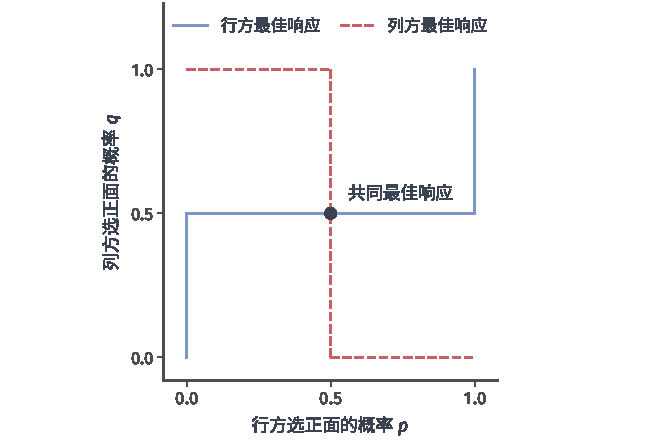
\includegraphics[width=\linewidth]{figures/01-mathematical-preliminaries/05-dynamical-systems-control-decision-and-games/matplotlib/game-matching-best-responses/figure.pdf}
  \caption{匹配硬币的最佳响应集合。横轴$p$、纵轴$q$分别是两方选$H$的概率。
  蓝色实线为行方响应，红色虚线为列方响应；在$q=1/2$处行方允许全部$p$，
  在$p=1/2$处列方允许全部$q$，唯一共同点为$(1/2,1/2)$。
  这些线段描述允许的响应，不是实际运行的学习轨迹。}
  \label{fig:game-matching-best-responses}
\end{figure}

三张牌中，固定应对概率\(c\)后，高牌质询的收益\(1+c\)总大于放弃的\(0\)，
故\(b_H=1\)是最佳选择。低牌质询收益为\(1-3c\)，所以\(c<1/3\)时选\(b_L=1\)，
\(c>1/3\)时选\(b_L=0\)，等于阈值时任意混合都可以。
反过来，由式~\eqref{eq:game-card-behavior-payoff}关于\(c\)的系数
\((b_H-3b_L)/2\)，列方在\(b_H>3b_L\)时选\(c=0\)，在\(b_H<3b_L\)时选\(c=1\)，
相等时任意\(c\)都最佳。这里比较的应对概率对两种隐藏牌必须相同，不能越过信息限制。

对温度一步成本，固定\(u_j\)后严格凸性给出唯一响应。求导并令导数为零：
\[
  \frac{\partial J_i}{\partial u_i}
  =2(0.8x+u_i+u_j-r_i)+2\lambda_i u_i=0.
\]
于是
\begin{equation}
  B_i(u_j;x)=\frac{r_i-0.8x-u_j}{1+\lambda_i}.
  \label{eq:game-heater-best-response}
\end{equation}
在\(x=0,r_i=2,\lambda_i=1\)时，对方取\(0.8\)，本人就愿意改为\(0.6\)。
即使\((0.8,0.8)\)使两人成本都低于某个其他方案，也不能据此称它为相互最佳响应。
若要求\(0\leq u_i\leq1\)，该二次成本的响应变为将右侧截到\([0,1]\)；
若还要求下一状态在\([0,3]\)，可行区间还依赖对方行动，须重新核对共同可行性。

\subsection{相互最佳响应下的Nash均衡}
\label{sec:game-nash}

\subsubsection{单方偏离与Nash条件}
\label{sec:game-nash-condition}

只求一人的响应仍没有决定联合结果。把每人的最佳响应条件同时写下，就得到
\term{Nash均衡}（Nash equilibrium）：只要其他人不变，没有谁能靠单独改策略提高收益。
\begin{definition}[Nash均衡]
\label{def:game-nash-equilibrium}
联合混合策略\(\bm\sigma^\star\)是Nash均衡，若对每个参与者\(i\)及每个可实施的
替代策略\(\widetilde{\bm\sigma}_i\)，
\begin{equation}
  u_i(\bm\sigma_i^\star,\bm\sigma_{-i}^\star)
  \geq u_i(\widetilde{\bm\sigma}_i,\bm\sigma_{-i}^\star).
  \label{eq:game-nash-no-unilateral-deviation}
\end{equation}
\end{definition}
等价地，各方最大单方改进
\(\max_{\widetilde{\bm\sigma}_i}u_i(\widetilde{\bm\sigma}_i,\bm\sigma_{-i}^\star)
-u_i(\bm\sigma^\star)\)均为零。每人都采用纯行动时称纯策略均衡，否则使用混合策略。
匹配硬币没有纯均衡：两面相同则第2方愿意改，不同则第1方愿意改；唯一混合均衡为
\(p=q=1/2\)，收益为零。

三张牌的同时响应要求\(b_H=1\)、\(b_L=1/3\)、\(c=1/3\)。
零和保证值的证书将在第~\ref{sec:game-matrix-zero-sum-duality}节独立核验。
温度一步例则解
\(2u_1+u_2=2,\ u_1+2u_2=2\)，得到唯一解
\[
  u_1^\star=u_2^\star=\frac23,\qquad x_1=\frac43,\qquad J_i^\star=\frac89.
\]
双方都不愿独改，但共同改成\((0.8,0.8)\)可把两人成本降为\(0.8<8/9\)。
事实上总成本\(2(u_1+u_2-2)^2+u_1^2+u_2^2\)严格凸，其梯度为零恰给出
\((0.8,0.8)\)。Nash条件不等于总成本最优或Pareto最优，也不比较不同均衡的公平性。
这里的\(x_1\)是从\(x_0=0\)开始的一步结果，不是闭环系统的稳态温度。

\subsubsection{响应映射与均衡存在}
\label{sec:game-equilibrium-existence}

% Baseline B:401-417
若每个最佳响应都是唯一且连续的，就可以把所有人的响应拼成映射
\[
  B(\bm{\sigma})
  =
  \bigl(
    \operatorname{BR}_1(\bm{\sigma}_{-1}),\ldots,
    \operatorname{BR}_n(\bm{\sigma}_{-n})
  \bigr),
\]
再寻找\(B(\bm{\sigma})=\bm{\sigma}\)。实际博弈常在收益并列处有多个最佳响应，
\(B\)因而不是单值连续函数。强行规定“并列时选编号最小的行动”会造成跳跃，不能直接
应用Brouwer不动点定理。

存在性论证需要两个不同层次的工具。连续单值映射先借助边界计数取得不动点；
最佳响应存在并列时，再用闭图和凸值保留整组选择。下面保留这两条工具的证明，
并在最后逐项核对有限博弈是否满足条件。
% Baseline B:420-500
\begin{lemma}[Sperner引理]
\label{lem:game-sperner}
把\(d\)维标准单纯形
\[
  \Delta^d
  =
  \left\{
    \bm{x}\in\mathbb{R}^{d+1}:
    \bm{x}\geq\bm{0},\
    \bm{1}^{\top}\bm{x}=1
  \right\}
\]
有限剖分成小单纯形。若每个剖分顶点的标签属于
\(\{0,\ldots,d\}\)，并且位于由顶点集合\(S\)张成的面上的点只能使用\(S\)中的
标签，则同时含有全部\(d+1\)种标签的小单纯形有奇数个，因而至少存在一个。
\end{lemma}

\begin{proof}
零维单纯形只有一个顶点，结论直接成立。对正维数\(d\)归纳。
\(d=1\)时，线段两个端点分别只能标\(0\)与\(1\)。沿剖分顶点
从左向右读取标签，每次改变对应一条含有两种标签的小线段；由于起点为\(0\)、终点为
\(1\)，改变次数为奇数。

先在\(d=2\)的三角形中看清高维计数。三条边上的剖分顶点只能使用相应两个端点的
标签。例如，顶点\(0\)与\(1\)之间的边只能标\(0\)或\(1\)，一维情形说明这条
边上含两种标签的小边有奇数条。计数所有带标签\(0,1\)的小边与小三角形的邻接：
内部小边被两个小三角形共享，贡献两次；大三角形边界上的小边只邻接一个小三角形，
而带齐\(0,1\)的边界小边只能出现在刚才的\(0,1\)边上。一个全标号小三角形恰有
一条\(0,1\)边，只含标签\(0,1\)且两种标签都出现的小三角形有两条这样的边，其余
小三角形没有。因此邻接总数为奇数迫使全标号小三角形的数量为奇数。一般维证明把
“小边”换成余维一的小面，把“小三角形”换成小单纯形。

假设结论对\(d-1\)维成立。在全部\(d\)维小单纯形中，计数标签集合恰为
\(\{0,\ldots,d-1\}\)的\((d-1)\)维面与小单纯形的邻接次数。内部面邻接两个
小单纯形，贡献偶数；边界面只邻接一个小单纯形。边界上只有大单纯形的
\(x_d=0\)面可能出现全部标签\(0,\ldots,d-1\)，因为其他边界面缺少其中某个允许
标签。该面继承Sperner标号，归纳假设说明其中这类小面有奇数个。因此总邻接次数为
奇数。

一个\(d\)维小单纯形若含有全部标签\(0,\ldots,d\)，恰有一个面带齐
\(0,\ldots,d-1\)，即去掉标签\(d\)顶点所得的面。若它没有标签\(d\)，却带齐
\(0,\ldots,d-1\)，则\(d+1\)个顶点中恰有一个标签重复，去掉任一重复标签顶点都会
得到这样的面，所以贡献两次；其余小单纯形贡献零次。总邻接次数的奇偶性因而等于全标号
小单纯形数目的奇偶性。前者为奇数，后者至少为一。
\end{proof}

\begin{theorem}[Brouwer不动点定理]
\label{thm:game-brouwer}
若\(K\subseteq\mathbb{R}^d\)非空、紧且凸，则每个连续映射
\(f:K\to K\)至少有一个不动点。
\end{theorem}

\begin{proof}
先令\(K=\Delta^d\)。取网格直径趋于零的一列单纯形剖分。若某个剖分顶点
\(\bm{x}\)已经满足\(f(\bm{x})=\bm{x}\)，结论成立；否则因为
\(\sum_jx_j=\sum_jf_j(\bm{x})=1\)，至少存在一个坐标\(j\)满足
\(x_j>f_j(\bm{x})\)，任选这样的\(j\)作为标签。若\(x_j=0\)，这个严格不等式
不可能成立，所以边界标号满足引理~\ref{lem:game-sperner}的条件。

每个剖分因而都有一个全标号小单纯形。对第\(k\)次剖分，记其中标签为\(j\)的顶点为
\(\bm{x}_{k,j}\)。由紧性可取子列，使\(\bm{x}_{k,0}\to\bm{x}^\star\)；小单纯形
直径趋于零，所以每个\(\bm{x}_{k,j}\)都趋于同一个\(\bm{x}^\star\)。标签定义和
连续性给出
\[
  x_j^\star\geq f_j(\bm{x}^\star),
  \qquad j=0,\ldots,d.
\]
两边坐标和都为\(1\)，故所有不等式只能同时取等号，
\(f(\bm{x}^\star)=\bm{x}^\star\)。

对一般的非空紧凸集\(K\)，取一个包含\(K\)的有限维单纯形\(S\)，并记
\(\Pi_K:S\to K\)为到闭凸集\(K\)的欧氏投影。映射
\(g=f\circ\Pi_K:S\to K\subseteq S\)连续，前一部分给出
\(\bm{x}^\star=g(\bm{x}^\star)\)。右侧属于\(K\)，所以
\(\bm{x}^\star\in K\)且\(\Pi_K(\bm{x}^\star)=\bm{x}^\star\)，进而
\(f(\bm{x}^\star)=\bm{x}^\star\)。
\end{proof}

在区间上，这个结论退化为对\(f(x)-x\)使用介值性质；高维中没有统一的“左右端点”，
Sperner引理用边界相容标号和奇偶计数补上了这一步。Brouwer只保证不动点存在，不要求
映射压缩，因此既不保证不动点唯一，也不保证反复应用\(f\)会收敛。
% Baseline B:503-533
需要的替代对象保留全部并列响应，不强制挑选其中一个。与单值连续性相应的条件，
要求附近输入的响应不能突然出现远离当前响应集合的新值。
\begin{definition}[集合值映射与上半连续性]
\label{def:game-upper-hemicontinuous-correspondence}
设$K\subseteq\mathbb R^d$非空且紧。\term{集合值映射}（correspondence）
\(F:K\rightrightarrows K\)给每个$x\in K$指定集合$F(x)\subseteq K$；本节要求各值非空。
若对每个$x\in K$及包含$F(x)$的相对开集$O\subseteq K$，都有$x$的相对邻域$U$，
使$F(z)\subseteq O$对所有$z\in U$成立，则称$F$\term{上半连续}（upper hemicontinuous）。
\end{definition}
在当前紧域、紧值的情形，一个便于使用的等价判据是闭图性质：
\[
  x_k\to x,\quad y_k\to y,\quad y_k\in F(x_k)
  \quad\Longrightarrow\quad
  y\in F(x).
\]
闭图判据适用于后面的有限博弈，因为定义域和值域都位于有限维紧集。

这个等价关系也可以直接核对。若闭图成立而上半连续失败，就有包含\(F(x)\)的
相对开集\(O\)，以及\(x_k\to x\)、\(y_k\in F(x_k)\setminus O\)。
紧性给出\(y_k\)的收敛子列，其极限仍在闭集\(K\setminus O\)，闭图却要求极限在
\(F(x)\subset O\)，矛盾。反过来，设上半连续且各值紧，若图中的点
\((x_k,y_k)\to(x,y)\)而\(y\notin F(x)\)，紧值与\(y\)的距离为正。
可取包含\(F(x)\)且与\(y\)的某邻域不交的相对开集；上半连续迫使最终的\(y_k\)
留在前者，收敛却迫使它们进入后者，再次矛盾。

例如，对手以概率\(q\)选择左列，而某参与者的两个行动收益分别为\(q\)和\(1-q\)时，
其最佳响应对应为
\[
  \operatorname{BR}(q)
  =
  \begin{cases}
    \{\text{左}\},&q>1/2,\\
    \Delta(\{\text{左},\text{右}\}),&q=1/2,\\
    \{\text{右}\},&q<1/2.
  \end{cases}
\]
在\(q=1/2\)强行挑一个行动会造成单值选择跳跃；保留整段混合策略后，对应的值仍非空、
紧且凸，并且极限不会跳出图。这正是Kakutani定理保留并列响应的方式。
% Baseline B:536-629
闭图控制极限，凸值允许在网格上混合相邻选择。二者配合，才可以把连续映射的存在工具
扩展到集合值响应，而不是对某个不连续的并列选择直接迭代。
下面使用的多值映射不动点结论源于Kakutani定理\scite{math-kakutani1941fixed}
\begin{theorem}[Kakutani不动点定理]
\label{thm:game-kakutani}
设\(K\subseteq\mathbb{R}^d\)非空、紧且凸。若
\(F:K\rightrightarrows K\)上半连续，并且每个\(F(x)\)都非空、紧且凸，
则存在\(x^\star\in K\)满足\(x^\star\in F(x^\star)\)。
\end{theorem}

下面用单纯形细分和重心插值，把集合值映射转为Brouwer定理能够处理的连续映射。

\begin{lemma}[单纯形上的连续近似选择]
\label{lem:game-approximate-selection}
在定理~\ref{thm:game-kakutani}的条件下，取一个包含\(K\)的单纯形
\(S\subseteq\mathbb{R}^d\)，并记到\(K\)的欧氏投影为
\(\Pi_K:S\to K\)。对每个\(\varepsilon>0\)，存在连续映射
\(f_\varepsilon:S\to K\)，使每个\(x\in S\)都有\(x'\in S\)及
\(y\in F(\Pi_K(x'))\)满足
\[
  \lVert x-x'\rVert_2
  +
  \lVert f_\varepsilon(x)-y\rVert_2
  <\varepsilon.
\]
\end{lemma}

\begin{proof}
对\(S\)取一列网格直径趋于零的有限单纯形细分。固定第\(k\)次细分；对每个网格顶点
\(\bm{v}\)，从非空集合\(F(\Pi_K(\bm{v}))\)中任选一点
\(\bm{y}_{\bm{v}}\)。若\(\bm{x}\)位于顶点为
\(\bm{v}_0,\ldots,\bm{v}_d\)的一个小单纯形内，把它写成重心坐标
\[
  \bm{x}
  =
  \sum_{j=0}^{d}\lambda_j\bm{v}_j,
  \qquad
  \lambda_j\geq0,\quad
  \sum_{j=0}^{d}\lambda_j=1,
\]
并定义
\[
  f_k(\bm{x})
  =
  \sum_{j=0}^{d}\lambda_j\bm{y}_{\bm{v}_j}.
\]
相邻小单纯形在公共面上使用相同的顶点值，所以这些仿射片段拼成连续映射。又因
\(K\)凸，每个\(f_k(\bm{x})\)都属于\(K\)。

在乘积空间上使用
\(\lVert(\bm{x},\bm{y})\rVert
=\lVert\bm{x}\rVert_2+\lVert\bm{y}\rVert_2\)。
下面说明网格变细时，\((\bm{x},f_k(\bm{x}))\)会一致逼近对应
\[
  \widetilde F(\bm{x})
  =
  F(\Pi_K(\bm{x}))
\]
的图。否则存在\(\varepsilon_0>0\)和点\(\bm{x}_k\in S\)，使这些点到
\(\operatorname{graph}(\widetilde F)\)的距离始终至少为\(\varepsilon_0\)。
取包含\(\bm{x}_k\)的小单纯形及其顶点
\(\bm{v}_{k,0},\ldots,\bm{v}_{k,d}\)。由\(S\)与\(K\)的紧性，可沿一个子列令
\(\bm{x}_k\to\bm{x}\)、各重心系数收敛，并令所选的
\(\bm{y}_{k,j}\in F(\Pi_K(\bm{v}_{k,j}))\)逐项收敛到\(\bm{y}_j\)。
网格直径趋于零，所以每个\(\bm{v}_{k,j}\to\bm{x}\)；投影连续和\(F\)的闭图性质
于是给出
\[
  \bm{y}_j\in F(\Pi_K(\bm{x})).
\]
值集的凸性进一步说明重心极限
\(\bm{y}=\sum_j\lambda_j\bm{y}_j\)仍属于
\(F(\Pi_K(\bm{x}))\)。另一方面，
\(f_k(\bm{x}_k)\to\bm{y}\)，这与到图的距离保持在
\(\varepsilon_0\)以上矛盾。因此充分细的网格给出所需
\(f_\varepsilon\)。
\end{proof}

\begin{proof}[定理~\ref{thm:game-kakutani}的证明]
对\(\varepsilon_k\downarrow0\)，由引理~\ref{lem:game-approximate-selection}
得到连续映射\(f_k:S\to K\subseteq S\)。Brouwer不动点定理说明存在
\(x_k\in S\)使\(x_k=f_k(x_k)\)；由于右侧属于\(K\)，每个\(x_k\)其实都在
\(K\)中。\(K\)紧，所以某个子列收敛到\(x^\star\in K\)。

近似选择性质给出\(x_k'\in S\)与
\(y_k\in F(\Pi_K(x_k'))\)，使
\(\lVert x_k-x_k'\rVert_2+\lVert x_k-y_k\rVert_2\to0\)。因此同一子列上
\(\Pi_K(x_k')\to x^\star\)且\(y_k\to x^\star\)。\(F\)具有闭图，于是
\[
  x^\star\in F(x^\star).
\]
细分和重心插值把集合值问题变成连续单值问题，Brouwer提供近似不动点，紧性提供收敛
子列，闭图性质再把极限送回\(F\)。
\end{proof}
% Baseline B:632-686
Nash的不动点论证给出有限博弈的基本存在性结果\scite{math-nash1951noncooperative}
\begin{theorem}[有限博弈存在混合Nash均衡]
\label{thm:game-nash-existence}
每个参与者和每个行动集都有限的战略式博弈至少存在一个混合策略Nash均衡。
\end{theorem}

\begin{proof}
联合混合策略空间
\[
  K=\prod_{i=1}^{n}\Delta(A_i)
\]
是有限维非空紧凸集。定义联合最佳响应对应
\[
  F(\bm{\sigma})
  =
  \prod_{i=1}^{n}
  \operatorname{BR}_i(\bm{\sigma}_{-i}).
\]
对固定\(\bm{\sigma}_{-i}\)，收益关于
\(\bm{\sigma}_i\)连续，而概率单纯形紧，所以最大值达到，
\(\operatorname{BR}_i\)非空且紧。收益关于自身混合策略线性，两个最佳响应的
凸组合仍达到同一最大值，所以最佳响应值集是凸集。

还需核对闭图。设
\(\bm{\sigma}^{(k)}\to\bm{\sigma}\)，并且
\(\bm{\tau}_i^{(k)}\to\bm{\tau}_i\)，其中
\(\bm{\tau}_i^{(k)}
\in\operatorname{BR}_i(\bm{\sigma}_{-i}^{(k)})\)。对任意固定替代策略
\(\widetilde{\bm{\sigma}}_i\)，最佳响应性质给出
\[
  u_i(\bm{\tau}_i^{(k)},\bm{\sigma}_{-i}^{(k)})
  \geq
  u_i(\widetilde{\bm{\sigma}}_i,\bm{\sigma}_{-i}^{(k)}).
\]
有限博弈的期望收益是混合概率的多线性函数，因而连续。令\(k\to\infty\)，得到
\[
  u_i(\bm{\tau}_i,\bm{\sigma}_{-i})
  \geq
  u_i(\widetilde{\bm{\sigma}}_i,\bm{\sigma}_{-i}).
\]
这对所有替代策略成立，故
\(\bm{\tau}_i\in\operatorname{BR}_i(\bm{\sigma}_{-i})\)。
每个分量都具有闭图，有限乘积\(F\)也上半连续。

定理~\ref{thm:game-kakutani}给出
\(\bm{\sigma}^\star\in F(\bm{\sigma}^\star)\)。逐分量展开正是
\(\bm{\sigma}_i^\star
\in\operatorname{BR}_i(\bm{\sigma}_{-i}^\star)\)，也就是
式~\eqref{eq:game-nash-no-unilateral-deviation}。
\end{proof}

存在性没有给出唯一性、计算效率或学习动态收敛。即便收益矩阵很小，最佳响应也可能在
多个均衡之间切换；在“石头、剪刀、布”一类循环响应中，逐轮选择当前最佳纯行动甚至
不会收敛。第~\ref{chap:mathematical-analysis}章的压缩映射同时给出唯一不动点与
迭代收敛，而Kakutani只在更弱条件下给出至少一个不动点。这两种结论服务于不同问题。

\subsection{零和对抗下的保证与均衡}
\label{sec:game-matrix-zero-sum-duality}

均衡从双方同时响应出发；零和中还可以从一方防御所有对手策略出发。
三张牌矩阵的每行最小收益依次为\(0,1/2,-1,0\)，每列最大收益均为\(1\)。
所以只用纯计划，行方至多保证\(1/2\)，列方却只能将行方收益上界压至\(1\)；
不存在纯策略鞍点。允许混合以后，两种保证是否仍有缺口？
% Baseline B:152-274
第1位参与者在不知道对方将怎样响应时，希望最大化自己能够保证的最小收益：
\[
  \underline v
  =
  \max_{\bm{x}\in\Delta_m}
  \min_{\bm{y}\in\Delta_n}
  \bm{x}^{\top}\bm{M}\bm{y}.
\]
对固定\(\bm{x}\)，第2位参与者的目标关于\(\bm{y}\)线性，所以最小值在某个纯列
达到。因此
\[
  \min_{\bm{y}\in\Delta_n}
  \bm{x}^{\top}\bm{M}\bm{y}
  =
  \min_j(\bm{M}^{\top}\bm{x})_j.
\]
类似地，第2位参与者希望把第1位参与者的最大可得收益压低到
\[
  \overline v
  =
  \min_{\bm{y}\in\Delta_n}
  \max_{\bm{x}\in\Delta_m}
  \bm{x}^{\top}\bm{M}\bm{y}
  =
  \min_{\bm{y}\in\Delta_n}\max_i(\bm{M}\bm{y})_i.
\]

对任意\(\bm{x},\bm{y}\)，都有
\[
  \min_{\widetilde{\bm{y}}}
  u(\bm{x},\widetilde{\bm{y}})
  \leq
  u(\bm{x},\bm{y})
  \leq
  \max_{\widetilde{\bm{x}}}
  u(\widetilde{\bm{x}},\bm{y}).
\]
分别对左侧取最大、右侧取最小，得到
\(\underline v\leq\overline v\)。这只是弱极小极大关系。要证明有限零和博弈中
两者相等，还需要说明双方约束恰好构成一对线性规划。

\begin{theorem}[有限零和博弈的极小极大定理]
\label{thm:game-finite-minimax}
对任意有限收益矩阵\(\bm{M}\)，有
\begin{equation}
  \max_{\bm{x}\in\Delta_m}
  \min_{\bm{y}\in\Delta_n}
  \bm{x}^{\top}\bm{M}\bm{y}
  =
  \min_{\bm{y}\in\Delta_n}
  \max_{\bm{x}\in\Delta_m}
  \bm{x}^{\top}\bm{M}\bm{y}.
  \label{eq:game-minimax-equality}
\end{equation}
共同数值称为博弈值\(v^\star\)。等式两侧的最优解分别称为双方的极小极大策略。
\end{theorem}

\begin{proof}
引入第1位参与者要保证的收益下界\(v\)。条件
\((\bm{M}^{\top}\bm{x})_j\geq v\)对每一列成立，恰好表示任何纯列都不能把收益压到
\(v\)以下。第1位参与者的问题因此是
\begin{equation}
  \begin{aligned}
    \max_{\bm{x},v}\quad&v\\
    \text{s.t.}\quad&
      \bm{M}^{\top}\bm{x}\geq v\bm{1},\\
    &\bm{1}^{\top}\bm{x}=1,\qquad
      \bm{x}\geq\bm{0}.
  \end{aligned}
  \label{eq:game-row-player-lp}
\end{equation}
它的最优值正是\(\underline v\)。为第一组不等式引入非负乘子
\(\bm{y}\geq\bm{0}\)，为概率归一化引入自由乘子\(w\)。
把最大化问题写成上界形式后，其拉格朗日函数可整理为
\[
  \mathcal{L}(\bm{x},v;\bm{y},w)
  =
  v+\bm{y}^{\top}
  (\bm{M}^{\top}\bm{x}-v\bm{1})
  +w(1-\bm{1}^{\top}\bm{x}).
\]
若对自由变量\(v\)取上确界仍为有限值，必须有
\(\bm{1}^{\top}\bm{y}=1\)。若对\(\bm{x}\geq\bm{0}\)取上确界仍为有限值，
还必须有
\[
  \bm{M}\bm{y}\leq w\bm{1}.
\]
满足这些条件时，上确界等于\(w\)。于是对偶问题为
\begin{equation}
  \begin{aligned}
    \min_{\bm{y},w}\quad&w\\
    \text{s.t.}\quad&
      \bm{M}\bm{y}\leq w\bm{1},\\
    &\bm{1}^{\top}\bm{y}=1,\qquad
      \bm{y}\geq\bm{0}.
  \end{aligned}
  \label{eq:game-column-player-lp}
\end{equation}
它要求每个纯行的收益都不超过\(w\)，所以最优值正是\(\overline v\)。两个单纯形
都非空且紧，目标连续，因此式~\eqref{eq:game-row-player-lp}与
\eqref{eq:game-column-player-lp}都有有限最优解。第
\ref{thm:opt-lp-strong-duality}号定理给出原对偶最优值相等，即
\(\underline v=\overline v=v^\star\)。
\end{proof}

这个证明不只是交换了\(\max\)与\(\min\)。概率归一化把乘子变成对方的混合策略，
逐行动收益约束把对偶可行性变成“没有纯行动能突破当前上界”。强对偶才把两种单方
证书接成同一个博弈值。

若\(\bm{x}^\star\)与\(\bm{y}^\star\)分别是两侧最优策略，则对任意
\(\bm{x}\in\Delta_m\)、\(\bm{y}\in\Delta_n\)，
\begin{equation}
  u(\bm{x},\bm{y}^\star)
  \leq
  u(\bm{x}^\star,\bm{y}^\star)
  \leq
  u(\bm{x}^\star,\bm{y}).
  \label{eq:game-zero-sum-saddle}
\end{equation}
左侧来自\(\bm{y}^\star\)把所有行收益限制在\(v^\star\)以下，右侧来自
\(\bm{x}^\star\)对所有列保证至少\(v^\star\)。这就是混合策略上的鞍点条件。
博弈值由式~\eqref{eq:game-minimax-equality}唯一确定，但达到该值的策略可以不唯一；
把“值唯一”误读成“解唯一”，会遗漏并列最优行动形成的整个最优策略集合。

下面保留同一牌面博弈的原对偶最优证书，使数值结论不依赖“双方刚好无差异”的猜测。
% Baseline B:278-322
对式~\eqref{eq:game-card-normal-form}，令第1位参与者在计划
\((B,P)\)与\((B,B)\)上分别放置概率\(2/3\)与\(1/3\)，其余计划概率为零：
\[
  \bm{x}^\star
  =
  (0,2/3,0,1/3)^{\top}.
\]
面对退让列，期望收益为
\[
  \frac23\cdot\frac12+\frac13\cdot1
  =
  \frac23;
\]
面对应对列，期望收益为
\[
  \frac23\cdot1+\frac13\cdot0
  =
  \frac23.
\]
所以\((\bm{x}^\star,2/3)\)是式~\eqref{eq:game-row-player-lp}的可行解。

再令第2位参与者以概率\(2/3\)退让、以概率\(1/3\)应对：
\[
  \bm{y}^\star=(2/3,1/3)^{\top}.
\]
四个纯计划对它的收益依次为
\[
  0,\qquad
  \frac12\cdot\frac23+1\cdot\frac13=\frac23,\qquad
  \frac12\cdot\frac23-1\cdot\frac13=0,\qquad
  \frac23.
\]
没有一行超过\(2/3\)，所以\((\bm{y}^\star,2/3)\)是
式~\eqref{eq:game-column-player-lp}的可行解。弱对偶已经足以说明两者同时最优，
博弈值为\(v^\star=2/3\)。

从牌面条件看，这个混合计划等价于：拿到高牌总是质询，拿到低牌以概率\(1/3\)质询；
参与者2面对质询时以概率\(1/3\)应对。高牌的强行动掩护了低牌的偶尔质询，低牌的
存在又使应对者不能总是退让。这个解释依赖参与者2看不到牌面；第
~\ref{sec:game-extensive-information}节已把该信息限制写进历史树。

极小极大结论依赖零和结构。若退让、应对或交易产生了双方并不相反的成本，就不能再用
一个标量博弈值同时概括双方目标。此时仍可讨论最佳响应，但稳定性必须改用一般和均衡。
对于无限或连续行动集，有限维线性规划证明也不再直接适用；交换极大与极小通常还需要
非空紧凸策略集、收益连续以及相应的凸凹结构。

鞍点条件恰是双方的Nash条件：行方不能增加收益，列方不能降低行方收益。
反过来，任一零和Nash均衡也给出这组鞍点不等式，故其收益等于同一个博弈值。
博弈值限制最坏对手下的期望保证，不表示任一局实现的收益都等于该值。

\subsection{共同建议下的偏离与均衡}
\label{sec:game-correlated-deviations}

% Baseline B:690-785
Nash均衡要求各人的随机化彼此独立。若一个公共装置先抽取联合行动
\(\bm{A}\sim\mu\)，再分别向参与者发送建议，建议之间可以相关。关键问题变成：
参与者在看到自己的建议以后，是否愿意按建议行动。

\begin{definition}[粗相关均衡与相关均衡]
\label{def:game-coarse-correlated-equilibrium}
设$\mu$为有限战略式博弈中联合行动集$\prod_i A_i$上的概率分布。
分布\(\mu\)是\term{粗相关均衡}（coarse correlated equilibrium, CCE），若对
每个参与者\(i\)和任意固定行动\(a_i'\)，
\begin{equation}
  \mathbb{E}_{\bm{A}\sim\mu}[u_i(\bm{A})]
  \geq
  \mathbb{E}_{\bm{A}\sim\mu}
  [u_i(a_i',\bm{A}_{-i})].
  \label{eq:game-cce}
\end{equation}
偏离者必须在看到建议之前承诺改用同一个固定行动。若允许他看到建议\(A_i\)后按映射
\(\phi_i(A_i)\)改动，则要求
\begin{equation}
  \mathbb{E}_{\bm{A}\sim\mu}[u_i(\bm{A})]
  \geq
  \mathbb{E}_{\bm{A}\sim\mu}
  [u_i(\phi_i(A_i),\bm{A}_{-i})]
  \label{eq:game-correlated-equilibrium}
\end{equation}
对所有映射\(\phi_i:A_i\to A_i\)成立，这定义
\term{相关均衡}（correlated equilibrium, CE）。
\end{definition}

在有限行动集上，CE条件等价于对每对\(a_i,a_i'\in A_i\)要求
\begin{equation}
  \sum_{\bm{a}_{-i}}
  \mu(a_i,\bm{a}_{-i})
  \bigl[
    u_i(a_i,\bm{a}_{-i})
    -
    u_i(a_i',\bm{a}_{-i})
  \bigr]
  \geq0.
  \label{eq:game-ce-linear-constraints}
\end{equation}
它把“收到\(a_i\)建议后改成\(a_i'\)”的条件收益比较乘上收到该建议的概率，因此
\(\mu(A_i=a_i)=0\)时无需另外定义条件概率。CCE则把求和扩到全部\(a_i\)，对应
参与者在看见建议前就承诺使用固定的\(a_i'\)。这些都是关于\(\mu\)的线性不等式，
所以有限博弈的CE与CCE集合都是凸多面体。

相关均衡排除的偏离更丰富，所以每个CE都是CCE，反向不一定成立。独立乘积分布形式的
Nash均衡又是CE的特例。这个包含关系来自允许偏离的信息和时机，而不是来自三个名称的
“强弱等级”。具体地说，固定偏离是映射偏离的特例，所以CE条件蕴含CCE条件；在Nash
乘积分布中，对手行动与自己的建议独立，而自身混合策略支持集中的每个行动都是对
\(\bm{\sigma}_{-i}\)的最佳响应，故观察建议后改用任何行动都不能提高收益。

一个二行动协调博弈可以显示相关分布与独立随机化的差别。双方都选\(L\)或都选\(R\)
时各得\(2\)，行动不同时各得\(0\)。独立地以\(1/2\)选择两项是一个混合Nash均衡，
每人期望收益为\(1\)。公共装置若以\(1/2\)推荐\((L,L)\)、以\(1/2\)推荐
\((R,R)\)，每人期望收益为\(2\)，并且看到任一建议后偏离都会把收益降为\(0\)，
所以该分布是CE。它不是两个边缘分布的乘积，但只是相对于上述独立混合均衡改善共同
收益；该博弈的两个纯Nash均衡本来也各给双方收益\(2\)，CE并不保证优于每个Nash均衡。
第~\ref{sec:game-regret-cfr}节会看到，外部遗憾自然对应CCE，内部或交换遗憾才对应CE。

矩阵博弈中的联合分布也需要与各人的边缘分布区分。
表~\ref{tab:game-independent-correlated-actions}固定刚才协调博弈的收益和每人边缘
概率：两种制度下每人都以$1/2$选择$L$，但一个制度独立抽样，另一个制度共同推荐。
收益差来自行动间的相关性，并非某个参与者改变了单独的混合概率。
图~\ref{fig:game-correlated-mass}把两种联合概率逐格显示：独立制度仍会把一半质量放在
行动不一致的格子里，共同建议则把这部分质量移到对角线。只看两个边缘分布，无法
辨认这种差别；相关均衡的偏离检验也必须使用联合分布。
\begin{figure}[htbp]
  \centering
  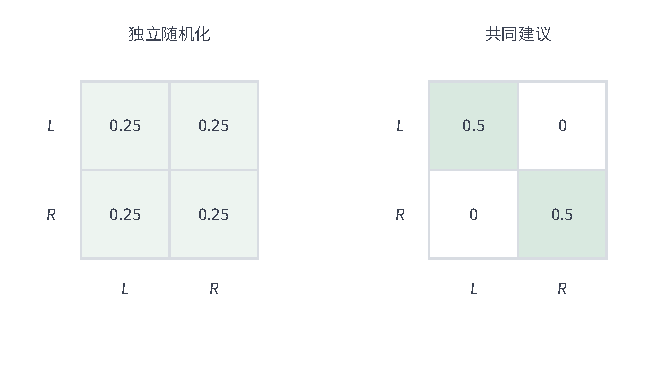
\includegraphics[width=\linewidth]{figures/01-mathematical-preliminaries/05-dynamical-systems-control-decision-and-games/tikz/game-correlated-mass/figure.pdf}
  \caption{二行动协调博弈的两个教学联合分布，共用$0$至$0.5$的概率色阶。
  行为参与者1的行动，列为参与者2的行动。左图为独立均匀策略，四格质量均为$0.25$；
  右图只推荐$(L,L)$与$(R,R)$，各占$0.5$。两者边缘概率均为$(0.5,0.5)$，
  但每人期望收益分别为$1$和$2$；相关分布并非边缘分布的乘积。}
  \label{fig:game-correlated-mass}
\end{figure}

\begin{table}[htbp]
  \centering
  \begin{tabular}{lcc}
    \toprule
    联合行动 & 独立混合概率 & 共同推荐概率\\
    \midrule
    $(L,L)$ & $1/4$ & $1/2$\\
    $(L,R)$ & $1/4$ & $0$\\
    $(R,L)$ & $1/4$ & $0$\\
    $(R,R)$ & $1/4$ & $1/2$\\
    \midrule
    每人的期望收益 & $1$ & $2$\\
    \bottomrule
  \end{tabular}
  \caption{同一边缘分布下的不同联合行动规律。教学协调博弈在相同行动时各得$2$，
  不同时各得$0$。右列是相关均衡，左列是独立混合Nash均衡；收益比较只针对这两个
  分布，纯策略协调均衡同样可以达到收益$2$。}
  \label{tab:game-independent-correlated-actions}
\end{table}

\subsection{合作分配下的偏离与稳定}
\label{sec:game-cooperative-deviation}

收益已经按贡献分配后，还须问成员愿不愿意留下来。这次允许偏离的单位可以是整个联盟，
而不只是一位参与者。这里的稳定指没有获利的退出与重组，不是策略更新对扰动的动态稳定。
% Baseline B:1838-1954
一个有效分配仍可能被某个联盟拒绝。若分配向量为\(\bm{x}\)，并满足
\[
  \sum_{i\in N}x_i=v(N),
\]
但存在联盟\(S\)使
\[
  \sum_{i\in S}x_i<v(S),
\]
那么该联盟单独合作可取得更多总收益。要求所有联盟都没有这种阻挡，并保持总收益完全
分配，得到一种对所有联盟的稳定性要求。
\begin{definition}[合作博弈的核心]
\label{def:game-cooperative-core}
对可转移效用博弈$(N,v)$，其\term{核心}（core）为分配向量$\bm x\in\mathbb R^{|N|}$的集合，
其中$\sum_{i\in N}x_i=v(N)$，并且$\sum_{i\in S}x_i\geq v(S)$对每个$S\subseteq N$成立。
\end{definition}
Shapley值不一定属于核心，核心也可能为空。
例如三人多数联盟的教学价值为$|S|\geq2$时$v(S)=1$，否则$v(S)=0$。
三人对称，Shapley值各为$1/3$；任意两人仅分到$2/3$，却能独立取得$1$，因此该分配不在核心。
更强地，三个两人联盟的不阻挡条件相加要求$2\sum_i x_i\geq3$，
有效性却要求$\sum_i x_i=1$，二者矛盾，所以核心为空。
前者由边际贡献平均和四项公理定义，后者由联盟偏离稳定性定义。

当收益不能转移时，应直接保留收益向量
\(\bm{u}(\bm{a})=(u_1(\bm{a}),\ldots,u_n(\bm{a}))\)。
第~\ref{sec:game-payoff-relations}节的Pareto条件只排除共同改进，通常形成一整个
前沿，并不选择其中哪一点。第~\ref{sec:opt-multiobjective-saddle}节中的共同下降
方向是一阶局部判据，也不能单独决定全局分配。

\begin{definition}[Nash乘积协商解]
\label{def:game-nash-bargaining-solution}
给定分歧点\(\bm{d}\in\mathbb R^n\)和可行收益集合\(U\subseteq\mathbb{R}^n\)，若下式的最大值达到，
\term{Nash协商解}（Nash bargaining solution）在参与者都不低于分歧收益的区域中
选择
\begin{equation}
  \max_{\bm{u}\in U,\ \bm{u}\geq\bm{d}}
  \prod_{i=1}^{n}(u_i-d_i),
  \label{eq:game-nash-bargaining}
\end{equation}
其中向量不等式逐坐标理解，称达到最大值的收益向量为协商解。
\end{definition}
分歧点表示谈判失败时每人的收益，因而乘积比较的是相对于
退出结果的增益，而不是原始收益本身。

\begin{theorem}[Nash乘积的存在、唯一性与Pareto性质]
\label{thm:game-nash-bargaining-properties}
设\(U\)非空、紧且凸，并存在\(\widehat{\bm{u}}\in U\)满足
\(\widehat{\bm{u}}>\bm{d}\)。则式~\eqref{eq:game-nash-bargaining}存在唯一的最优
收益向量\(\bm{u}^\star>\bm{d}\)，且\(\bm{u}^\star\)是Pareto最优的。若每位
参与者的效用与分歧收益同时作正仿射变换
\(u_i'=a_i u_i+b_i\)、\(d_i'=a_i d_i+b_i\)，其中\(a_i>0\)，变换后的解正是
\(\bm{u}^{\star\prime}=(a_i u_i^\star+b_i)_{i=1}^n\)。
\end{theorem}

\begin{proof}
个体可接受集合
\[
  K=U\cap\{\bm{u}:\bm{u}\geq\bm{d}\}
\]
非空且紧，乘积目标连续，所以最大值能够达到。严格可行点
\(\widehat{\bm{u}}\)的乘积为正，而任何至少一个坐标等于相应\(d_i\)的点乘积为
零，因此任一最优解都严格满足\(\bm{u}>\bm{d}\)。在这个正增益区域，最大化乘积
等价于最大化
\[
  F(\bm{u})=\sum_{i=1}^{n}\log(u_i-d_i).
\]
每个对数项在其坐标上严格凹，故\(F\)在正增益区域严格凹。若有两个不同最优点，凸性
保证它们的中点仍在\(U\)内，严格凹性却使中点目标严格大于两端，产生矛盾。因此最优
收益向量唯一。

若存在\(\widetilde{\bm{u}}\in U\)使
\(\widetilde{\bm{u}}\geq\bm{u}^\star\)且至少一个坐标严格更大，则所有增益保持为
正，乘积严格增加，与最优性矛盾，所以\(\bm{u}^\star\)是Pareto最优的。正仿射
变换后，每个增益变为
\(u_i'-d_i'=a_i(u_i-d_i)\)，整个乘积只乘上与候选点无关的正常数
\(\prod_i a_i\)。可行收益集合与最优点按同一坐标变换对应，因而最优选择不变。
\end{proof}

例如，两位参与者的可行收益满足
\[
  U=\{(u_1,u_2):u_1\geq0,\ u_2\geq0,\ u_1+u_2\leq6\},
  \qquad
  \bm{d}=(1,1).
\]
任何最优点都在边界\(u_1+u_2=6\)上，否则还能同时增加收益。令
\(x=u_1-1\)，则\(u_2-1=4-x\)，Nash乘积为
\[
  x(4-x)=4-(x-2)^2,
\]
故唯一解为\((u_1^\star,u_2^\star)=(3,3)\)。若只把分歧点改为\((0,1)\)，
边界上的乘积变为\(u_1(5-u_1)\)，解随之变成\((5/2,7/2)\)。这个算例说明，
协商解的“公平”相对于明确的退出收益而言，并不是脱离分歧点的绝对均分。

图~\ref{fig:game-bargaining-disagreement}将两个分歧点与对应最优收益画在同一可行
区域中。两次最优点都落在同一Pareto边界上，但分歧点改变后，乘积是在另一组增益
坐标中计算，因此最优位置也改变。唯一性来自固定可行域和固定分歧点下的严格凹目标，
不表示所有协商制度都应该选同一个收益向量。

\begin{figure*}[htbp]
  \centering
  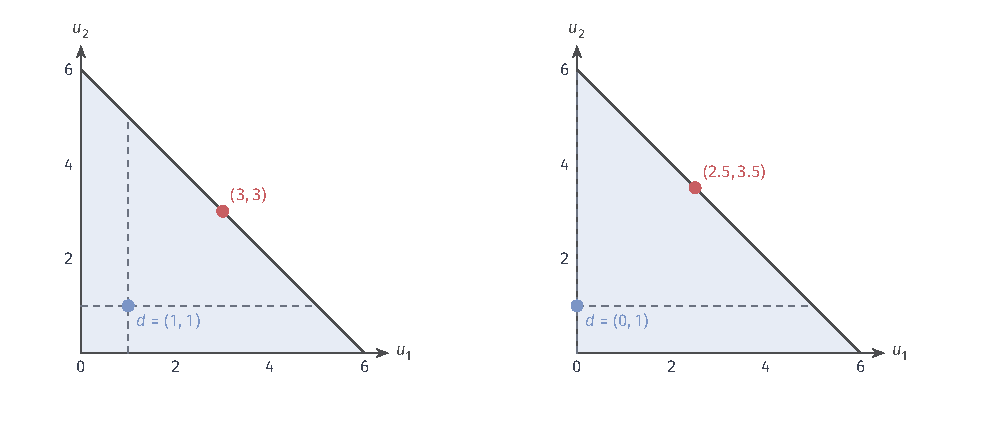
\includegraphics[width=\linewidth]{figures/01-mathematical-preliminaries/05-dynamical-systems-control-decision-and-games/tikz/game-bargaining-disagreement/figure.pdf}
  \caption{两方协商的教学可行域$u_1,u_2\geq0$、$u_1+u_2\leq6$，两图坐标一致。
  蓝点为分歧收益，红点为相对该分歧点的Nash乘积最优解。左图$\bm d=(1,1)$得到
  $(3,3)$，右图$\bm d=(0,1)$得到$(2.5,3.5)$；灰色虚线给出个体可接受的下界。
  可行总收益没有变化，变化的是退出时可得到的收益。}
  \label{fig:game-bargaining-disagreement}
\end{figure*}

没有共同严格正增益时，对数证明不适用，乘积还可能在多个零增益点同时达到最大；若
\(U\)非凸，严格凹性也不能排除不同连通部分上的多个最优点。改变分歧点会改变解，收益
若作一般非线性变换，乘积比较同样会改变。这个“协商解”与非合作博弈中的“Nash均衡”
共享提出者姓名，却解决不同问题。

至此，单方策略偏离、依建议改动和联盟退出都有了各自的比较条件。
这些条件检验一个候选结果是否会被拒绝，却没有给出参与者从初始选择走向该结果的过程。
要研究调整以后会不会回到附近、长期会不会停下来，还需要明确下一轮怎样更新。

\section{策略的多方演化与稳定}
\label{sec:game-policy-evolution}

同一个博弈可以配上不同的调整过程。双方可以同时回应上一轮，也可以轮流回应对方刚
作出的选择；可以每次求精确最优，也可以只沿当前收益增加的方向移动一小步。
这些过程共享收益函数，却不共享轨迹。因而必须先写出更新，才能讨论均衡附近的扰动
或长期极限。

\subsection{更新规则与策略序列}
\label{sec:game-update-sequences}

用\(t\)表示一局内的物理时间，用\(k=0,1,\ldots\)表示策略更新轮次。第\(k\)轮的
联合策略为\(\bm\sigma^{(k)}\)，该轮温度轨迹若需同时标明两种索引，可写成
\(x_t^{(k)}\)。本节比较相同初态、收益和信息条件下的更新；若每轮初态也变化，
就须把它纳入更新输入，不能直接套用下面的固定映射。
一般形式为
\[
  \bm\sigma^{(k+1)}
  =F_k\bigl(\bm\sigma^{(k)},\mathcal H^{(k)},\bm\xi^{(k)}\bigr),
\]
其中\(\mathcal H^{(k)}\)是更新时可用的历史信息，\(\bm\xi^{(k)}\)包括抽样或估计
噪声。即使局内策略采用随机行动，精确期望收益下的跨轮更新仍可能是确定的。
若使用累计遗憾、历史平均或动量，当前策略本身不足以决定下一步，须把这些内部量一并
放进动态系统的状态。下面先研究不显含\(k\)、无噪声的映射。

两方的同时最佳响应使用同一个旧组合：
\begin{equation}
  \sigma_1^{(k+1)}\in\operatorname{BR}_1(\sigma_2^{(k)}),
  \qquad
  \sigma_2^{(k+1)}\in\operatorname{BR}_2(\sigma_1^{(k)}).
  \label{eq:game-simultaneous-best-response}
\end{equation}
若有并列最优，这只是集合值规则，还须声明怎样选择响应。交替更新把一轮定义为两次
依次调整：
\begin{equation}
  \sigma_1^{(k+1)}\in\operatorname{BR}_1(\sigma_2^{(k)}),
  \qquad
  \sigma_2^{(k+1)}\in\operatorname{BR}_2(\sigma_1^{(k+1)}).
  \label{eq:game-alternating-best-response}
\end{equation}
第二方使用新信息，所以两式不是同一个联合映射。实际异步系统若使用延迟观测，
还要把延迟写出来。

精确响应可能代价很高。若第\(i\)方策略由
\(\bm\theta_i\in C_i\)参数化、\(C_i\)非空闭凸，且收益对该参数可微，可采用
\begin{equation}
  \bm\theta_i^{(k+1)}
  =\Pi_{C_i}\left(
    \bm\theta_i^{(k)}
    +\eta_i^{(k)}
    \nabla_{\bm\theta_i}u_i(\bm\theta^{(k)})
  \right).
  \label{eq:game-simultaneous-gradient}
\end{equation}
这是收益梯度上升；若写成本\(J_i=-u_i\)，符号改为下降。
概率单纯形上的投影保持非负与归一化，但不会自动使对方收益改善，也不保证联合映射
收缩。第~\ref{sec:game-projection-regret}节将在凸损失、梯度界和明确反馈条件下
证明它的累计保证。用估计梯度替代真梯度时，估计何时形成、是否条件无偏、方差是否
受控都是额外假设，不包含在上式的确定性分析中。

两方加热的一步模型使更新次序可以直接计算。固定\(x=0,r_1=r_2=2\)、
\(\lambda_1=\lambda_2=1\)，把每轮重新选择的一步输入写成
\(\bm u^{(k)}=(u_1^{(k)},u_2^{(k)})^\top\)，而非局内输入\(u_{i,t}\)。
由第~\ref{sec:game-best-response}节的响应公式，
\[
  B_1(u_2)=1-\frac12u_2,\qquad
  B_2(u_1)=1-\frac12u_1.
\]
同时更新从\((0,0)\)出发依次得到
\[
  (0,0),\quad (1,1),\quad (1/2,1/2),\quad(3/4,3/4),\ldots;
\]
交替更新从同一点出发，一轮结束时则依次为
\[
  (0,0),\quad(1,1/2),\quad(3/4,5/8),\quad(11/16,21/32),\ldots.
\]
两者都可能趋向\((2/3,2/3)\)，但不能凭前几个数确认收敛；下面给出误差递推。

\subsection{均衡邻域内的扰动与稳定}
\label{sec:game-local-stability}

对确定的联合映射\(F\)，先检查候选均衡\(\bm\theta^\star\)是否满足
\(F(\bm\theta^\star)=\bm\theta^\star\)。精确最佳响应若在均衡处选择当前策略，
这个条件成立；若任意打破并列最优，所选映射却可能把均衡点移走。投影梯度的不动点
只给出各方的一阶条件，只有各方收益关于自身策略凹等条件成立时，才足以推出最佳响应。
因此更新不动点与Nash均衡不能无条件等同。

在此前提下，稳定问的是初始微小偏差会不会一直小，渐近稳定还要求偏差最终趋零。
第~\ref{chap:dynamical-systems-and-state-estimation}章的定义现在应用于策略，而不是房间温度。
在内点的局部坐标中，若\(F\)连续可微，令
\(\bm e^{(k)}=\bm\theta^{(k)}-\bm\theta^\star\)，则
\[
  \bm e^{(k+1)}
  =\bm J_F(\bm\theta^\star)\bm e^{(k)}
    +o(\|\bm e^{(k)}\|).
\]
若谱半径\(\rho(\bm J_F(\bm\theta^\star))<1\)，可选一个等价向量范数，
使该矩阵的诱导范数小于\(1\)。由导数连续性，足够小邻域内的映射仍严格收缩；
取以不动点为中心的更小闭球便得到不变邻域和几何衰减。因此这是局部渐近稳定的
充分条件。若存在模大于\(1\)的特征值，光滑离散系统的线性化不稳定判据适用；
若有模等于\(1\)的特征值，一阶展开本身不作决定，须检查高阶项或其他不变量。
谱半径小于\(1\)也不要求欧氏距离每一步都下降，非正规矩阵可以先出现瞬态增长。

单纯形上的内点可先去掉一个由归一化决定的坐标，在线性切空间中应用这一判断。
边界处投影可能不可微；并列最佳响应可能发生跳变，集合值响应甚至没有普通Jacobian。
此时应直接验证距离不等式、可行方向或相应集合值条件，不能把内点判据强行套在边界上。

对加热例，令\(\bm e^{(k)}=\bm u^{(k)}-(2/3,2/3)^\top\)。同时响应恰好满足
\begin{equation}
  \bm e^{(k+1)}
  =
  \begin{pmatrix}0&-1/2\\-1/2&0\end{pmatrix}\bm e^{(k)}.
  \label{eq:game-heater-response-error}
\end{equation}
特征值为\(1/2,-1/2\)，且每轮欧氏误差恰好缩为一半。交替响应给出
\[
  \bm e^{(k+1)}
  =
  \begin{pmatrix}0&-1/2\\0&1/4\end{pmatrix}\bm e^{(k)},
\]
特征值为\(0,1/4\)。两个线性递推都对任意初值收敛，因而此处的结论不只局部成立。
它们收敛到的是固定初态的一步Nash输入，不是共同最优输入，也不意味着下一局温度
自动稳定在\(2\)。

同一成本若改用同时梯度下降，梯度向量为
\[
  \bm g(\bm u)=
  \begin{pmatrix}4u_1+2u_2-4\\2u_1+4u_2-4\end{pmatrix}.
\]
固定步长\(\eta>0\)时，误差矩阵是
\(\bm I-\eta\left(\begin{smallmatrix}4&2\\2&4\end{smallmatrix}\right)\)，
特征值为\(1-6\eta,1-2\eta\)。所以\(0<\eta<1/3\)保证全局收敛；
\(\eta=1/3\)保留一个不衰减的交替方向，更大步长会放大该方向。
即使每个人的成本关于自身行动严格凸，也不能省去步长条件。

再与式~\eqref{eq:game-two-heater-dynamics}比较。固定反馈下的状态稳定条件是
\(|0.8-k_1-k_2|<1\)，其中\(k_i\)为反馈增益；上述策略更新的条件却由响应矩阵
或梯度步长决定。一个按局内时间\(t\)判断，一个按学习轮数\(k\)判断。
若把学习与状态演化同时运行，分析对象须扩成状态与学习内部量的联合系统，本节两项
分开的计算不能替代它。

\subsection{长期更新的极限与循环}
\label{sec:game-limits-cycles}

加热例说明特定响应确实收敛，匹配硬币则说明均衡存在不足以保证这一点。
以\((p^{(k)},q^{(k)})\)表示两人选\(H\)的概率。从纯组合\((1,1)\)出发，
式~\eqref{eq:game-simultaneous-best-response}唯一地给出
\[
  (1,1)\longmapsto(1,0)\longmapsto(0,0)
  \longmapsto(0,1)\longmapsto(1,1).
\]
每一步都在最佳回应上一轮，联合序列却是四周期。若改成交替响应，则从\((1,1)\)
经一轮到\((1,0)\)，再到\((0,1)\)，此后两个组合交替，也不趋向混合均衡。
这些轨迹没有涉及并列响应点，因此循环不是由模糊的择优约定造成的。

梯度小步也不能普遍消除对抗导致的旋转。在概率正方形的内部，对收益
\(u_1=(2p-1)(2q-1)\)、\(u_2=-u_1\)同时上升，令
\(a^{(k)}=p^{(k)}-1/2\)、\(b^{(k)}=q^{(k)}-1/2\)，得到
\[
  \begin{pmatrix}a^{(k+1)}\\b^{(k+1)}\end{pmatrix}
  =
  \begin{pmatrix}1&4\eta\\-4\eta&1\end{pmatrix}
  \begin{pmatrix}a^{(k)}\\b^{(k)}\end{pmatrix}.
\]
两个特征值为\(1\pm4\eta\mathrm i\)，模为
\(\sqrt{1+16\eta^2}>1\)。在投影尚未起作用时，平方半径每轮乘上
\(1+16\eta^2\)，所以任何正的固定步长都不能使中心局部吸引。
触及边界后的轨迹还取决于投影，不能把内部递推无限延长。
若改为连续学习时间\(\tau\)的梯度流
\(\dot a=4b,\dot b=-4a\)，则
\(\frac{\mathrm d}{\mathrm d\tau}(a^2+b^2)=0\)，得到闭合圆轨道。
这里的\(\tau\)不是局内物理时间\(t\)，也不是离散轮数\(k\)。

\begin{figure*}[htbp]
  \centering
  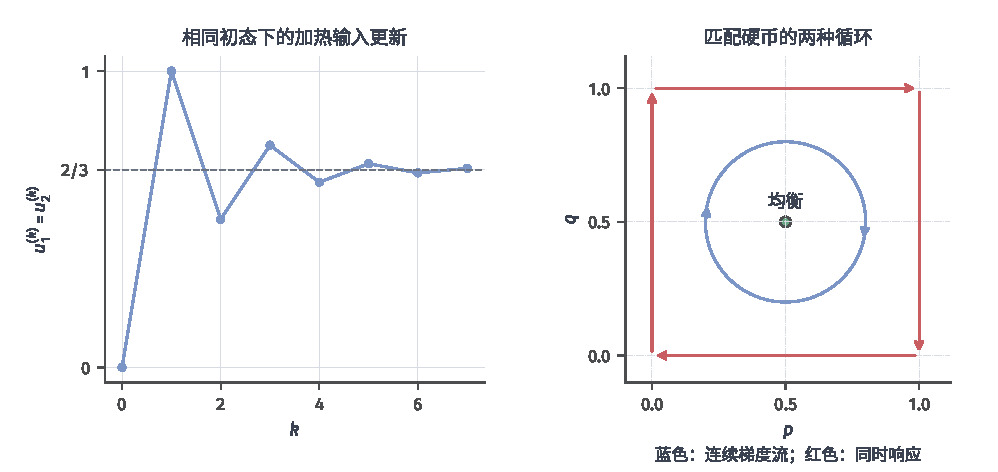
\includegraphics[width=\linewidth]{figures/01-mathematical-preliminaries/05-dynamical-systems-control-decision-and-games/matplotlib/game-update-trajectories/figure.pdf}
  \caption{两个已明确更新规则的教学轨迹。左图为相同初态下双加热器的同时最佳响应，
  从\(u_1^{(0)}=u_2^{(0)}=0\)开始，两条输入曲线重合，误差交替减半并趋向\(2/3\)。
  右图红色方形箭头是匹配硬币的离散四周期，蓝色圆是内部连续梯度流从
  \((p,q)=(0.8,0.5)\)出发的闭轨道，中心标记是Nash均衡。
  圆与方形对应不同更新，均不是最佳响应对应图中的静态集合。}
  \label{fig:game-update-trajectories}
\end{figure*}

多方演化还可以不以每个个体显式求梯度为出发点。若大量个体采用有限种行动，
收益较高的类型在下一时刻占更大比例，就得到按相对收益调整比例的
\term{复制动态}（replicator dynamics）。
在一个对称双人群体博弈中，设收益矩阵为\(\bm A\)，群体比例
\(\bm p(\tau)\in\Delta_m\)，类型\(a\)面对群体的收益为\((\bm A\bm p)_a\)，
平均收益为\(\bm p^\top\bm A\bm p\)。“对称”指交换参与者角色也交换收益，
即两方收益矩阵为\(\bm A,\bm A^\top\)，不要求\(\bm A\)本身是对称矩阵。
连续模型为
\begin{equation}
  \dot p_a
  =p_a\bigl[(\bm A\bm p)_a-\bm p^\top\bm A\bm p\bigr].
  \label{eq:game-replicator}
\end{equation}
各坐标导数之和为零，边界\(p_a=0\)上该坐标导数也为零，故单纯形保持不变。
正比例类型在静止点必须与群体平均收益相同，但未出现的类型仍可能有更高收益。
例如一个纯类型顶点总是静止点，却未必是Nash均衡；没有该类型的初始个体且没有
变异机制时，复制方程不会凭空引入它。

两方角色不同的匹配硬币应写成两个群体，而不是直接套单群体矩阵。两方复制动态为
\[
  \dot p=2p(1-p)(2q-1),\qquad
  \dot q=-2q(1-q)(2p-1).
\]
内部轨迹满足
\[
  \frac{\mathrm d}{\mathrm d\tau}
  \log\!\bigl[p(1-p)q(1-q)\bigr]=0.
\]
除中心外，每个内部水平集是围绕中心的闭曲线，向量场在其上不为零，因而形成周期运动。
这再次说明混合Nash不必吸引学习轨迹，但此处闭轨道一般不是梯度流的圆。

在对称单群体模型中，另一个问题是少量不同策略进入后能否扩张。
\begin{definition}[演化稳定策略]
\label{def:game-evolutionarily-stable}
设对称双人博弈中使用策略\(\bm p\)对阵\(\bm q\)的收益为
\(U(\bm p,\bm q)=\bm p^\top\bm A\bm q\)。
策略\(\bm p^\star\)是\term{演化稳定策略}（evolutionarily stable strategy, ESS），
若对每个\(\bm q\ne\bm p^\star\)，存在\(\bar\varepsilon(\bm q)>0\)，使所有
\(0<\varepsilon<\bar\varepsilon(\bm q)\)都满足
\[
  U(\bm p^\star,(1-\varepsilon)\bm p^\star+\varepsilon\bm q)
  >
  U(\bm q,(1-\varepsilon)\bm p^\star+\varepsilon\bm q).
\]
\end{definition}
左侧是原群体策略面对少量新策略时的收益，右侧是新策略在同一混合群体中的收益。
将两侧之差展开为
\[
  (1-\varepsilon)
  [U(\bm p^\star,\bm p^\star)-U(\bm q,\bm p^\star)]
  +\varepsilon[U(\bm p^\star,\bm q)-U(\bm q,\bm q)]
\]
可见，对每个\(\bm q\ne\bm p^\star\)，第一个括号必须为正，或在它为零时第二个
括号必须为正。这给出可直接计算的等价条件，也说明ESS必为对称Nash策略：
若第一个括号为负，再小的正入侵比例也不能满足定义。

例如\(\bm A=\left(\begin{smallmatrix}0&2\\2&0\end{smallmatrix}\right)\)，
\(\bm p^\star=(1/2,1/2)^\top\)。对任意\(\bm q=(q,1-q)^\top\)，
\[
  \begin{aligned}
    U(\bm p^\star,\bm p^\star)&=U(\bm q,\bm p^\star)=1,\\
    U(\bm p^\star,\bm q)-U(\bm q,\bm q)&=1-4q(1-q)\\
      &=(2q-1)^2.
  \end{aligned}
\]
因此\(\bm p^\star\)是ESS。此例复制动态为
\(\dot p=2p(1-p)(1-2p)\)：\(0<p<1/2\)时比例增加，\(1/2<p<1\)时减少，
所有内部初值都趋向\(1/2\)；线性化导数为\(-1\)，也证实局部吸引。
相反，两个顶点虽静止，却可被缺席类型侵入。
ESS检验少量策略入侵，动态稳定检验指定方程的扰动，Nash检验单方偏离；
这里同时成立的结论来自具体计算，不代表三种定义相同，也不涵盖有限群体随机漂移。

最后须说明“长期结果”指什么。逐轮策略是\(\bm\sigma^{(k)}\)，某个点的收敛是
\(\|\bm\sigma^{(k)}-\bm\sigma^\star\|\to0\)；接近均衡集合仅要求到该集合的距离
趋零，若集合不止一点，两者不同。有限矩阵策略的时间平均与实际行动经验分布分别为
\[
  \bar{\bm\sigma}_i^{(K)}
  =\frac1K\sum_{k=1}^K\bm\sigma_i^{(k)},\qquad
  \widehat\mu^{(K)}(\bm a)
  =\frac1K\sum_{k=1}^K\mathbb I\{\bm a^{(k)}=\bm a\}.
\]
若每轮只计算混合策略而不抽样，保留轮内独立性的对应联合平均是
\(\mu_{\mathrm{mix}}^{(K)}=K^{-1}\sum_k\bigotimes_i\bm\sigma_i^{(k)}\)，
通常不等于\(\bigotimes_i\bar{\bm\sigma}_i^{(K)}\)。
实际经验分布与这个混合分布平均之间还隔着抽样误差。
匹配硬币的四周期没有末项极限，但每满四轮，两方平均都为\((1/2,1/2)\)。
这只是该轨迹的计算结果，不能证明任意响应算法都有低遗憾。
反过来，即使已有低遗憾，也仍须说明它控制的是哪个平均对象。

\section{策略的多方累积表现}
\label{sec:game-regret-cfr}

策略没有停下来时，仍可问整个过程是否持续错过某个更好的固定选择。
遗憾把实际收益序列与同一评价序列下的替代策略比较：固定的是已经记录的对手策略，
不是假设自己改动以后对手会重新学习。若替代行为还会改变对手的后续响应，就须另建
反事实演化模型；本节基本遗憾界不比较两套重新运行的学习系统。

\subsection{固定比较策略下的累计差距}
\label{sec:game-regret-comparators}

先以损失说明符号，损失越小越好。离开当前时刻以后，回看前\(K\)轮，假设始终使用
同一个行动，它会比实际选择少付出多少损失？
\begin{definition}[外部遗憾]
\label{def:game-external-regret}
设行动集\(A\)非空且有限。同一参与者在第\(k\)轮选择\(a^{(k)}\)，面对损失函数
\(\ell^{(k)}:A\to\mathbb R\)。相对于事后最佳固定行动的
\term{外部遗憾}（external regret）为
\begin{equation}
  R_{\mathrm{ext}}^{(K)}
  =\max_{a\in A}\sum_{k=1}^K
    [\ell^{(k)}(a^{(k)})-\ell^{(k)}(a)].
  \label{eq:game-external-regret}
\end{equation}
\end{definition}
记\([z]_+=\max\{z,0\}\)。若
\([R_{\mathrm{ext}}^{(K)}]_+/K\to0\)，称该序列无外部遗憾，即平均每轮损失渐近
不高于任何固定行动。这里保留正部，是因为实际序列可能比所有固定行动都好，
使未经截断的遗憾为负；定义不要求它从负侧趋于零。
比较对象不是每轮先看到损失再重新选择的动态先知；后者通常能取得更小损失，
要对它给出累计保证，还需要变化预算或可预测性等条件。

例如两行动\(B,P\)的损失向量交替为\((0,1)\)、\((1,0)\)，共\(2m\)轮。
始终选择\(B\)的损失为\(m\)，最佳固定行动的损失也是\(m\)，外部遗憾为零；
每轮可预知损失的先知却能取得零损失，差距为\(m\)。
若每轮使用分布\(\bm w^{(k)}\)，则将实际项改为期望损失
\(\langle\bm w^{(k)},\bm\ell^{(k)}\rangle\)。
对任何固定混合分布，累计损失仍是其概率的线性函数，最小值在某个纯行动达到，
所以固定混合比较并未提高这类线性损失下的最优比较值。
但抽样行动的实际遗憾与分布的期望损失遗憾并非同一随机变量。

\begin{definition}[内部遗憾]
\label{def:game-internal-regret}
在同一行动损失序列下，\term{内部遗憾}（internal regret）允许把每次实际选择
\(a\)的轮次统一替换成另一行动\(b\)，对应差距为
\[
  R_{a\to b}^{(K)}
  =\sum_{k=1}^K\mathbb I\{a^{(k)}=a\}
    [\ell^{(k)}(a)-\ell^{(k)}(b)].
\]
对所有\((a,b)\in A\times A\)计算该量，其最大正部称为内部遗憾。
\end{definition}
控制所有这类差距，表示在知道“原本要选\(a\)”以后，也没有持续更好的统一替换。
对任意固定\(b\)，外部比较差距等于\(\sum_aR_{a\to b}^{(K)}\)；
故有限行动下无内部遗憾蕴含无外部遗憾，反向一般不成立。
这些比较分别对应相关均衡中按建议改动和粗相关均衡中的固定偏离。
改用收益\(u^{(k)}=-\ell^{(k)}\)时，遗憾写成替代收益减实际收益，正号仍表示
偏离有利，不能把两种约定混用。

\subsection{基于投影更新的累计保证}
\label{sec:game-projection-regret}

若每轮只需沿当前损失的下降方向调整，怎样控制所有轮次合起来的损失？
关键不是证明每轮都更接近当轮最优点，而是跟踪到同一个固定比较点的距离。
下面的次梯度界采用全信息或可取得真次梯度的反馈。

% Baseline B:1084-1185; learning indices normalized
第~\ref{sec:opt-projected-methods}节的投影不只用于离线优化，也能控制在线累计
损失\scite{math-zinkevich2003online}设\(C\subseteq\mathbb{R}^d\)为非空闭凸集，
直径至多为\(D\geq0\)，即对任意\(\bm{u},\bm{v}\in C\)都有
\(\lVert\bm{u}-\bm{v}\rVert_2\leq D\)。给定轮数\(K\geq1\)和步长\(\eta>0\)，
第\(k\)轮在选择
\(\bm{w}^{(k)}\in C\)后观察凸损失\(f^{(k)}\)，取次梯度
\(\bm{g}^{(k)}\in\partial f^{(k)}(\bm{w}^{(k)})\)，并假设
\(\lVert\bm{g}^{(k)}\rVert_2\leq G\)，其中\(G\geq0\)。在线投影次梯度更新为
\begin{equation}
  \bm{w}^{(k+1)}
  =
  \Pi_C\bigl(
    \bm{w}^{(k)}-\eta\bm{g}^{(k)}
  \bigr).
  \label{eq:game-online-projected-gradient}
\end{equation}

\begin{theorem}[在线投影次梯度的外部遗憾]
\label{thm:game-online-gradient-regret}
对任意比较点\(\bm{w}\in C\)，更新
\eqref{eq:game-online-projected-gradient}满足
\begin{equation}
  \sum_{k=1}^{K}
  \bigl(
    f^{(k)}(\bm{w}^{(k)})-f^{(k)}(\bm{w})
  \bigr)
  \leq
  \frac{D^2}{2\eta}
  +\frac{\eta G^2K}{2}.
  \label{eq:game-online-gradient-regret-bound}
\end{equation}
当\(D>0\)且\(G>0\)时，取\(\eta=D/(G\sqrt{K})\)，右侧为
\(DG\sqrt{K}\)。若\(D=0\)，则\(C\)只有一个点；若\(G=0\)，次梯度不等式说明
每轮差值都不大于零。两种退化情形的遗憾上界均为零，无需使用这个步长公式。
\end{theorem}

\begin{proof}
欧氏投影不会增加到任意可行点的距离，所以
\begin{align*}
  \lVert\bm{w}^{(k+1)}-\bm{w}\rVert_2^2
  &\leq
  \lVert
    \bm{w}^{(k)}-\eta\bm{g}^{(k)}-\bm{w}
  \rVert_2^2\\
  &=
  \lVert\bm{w}^{(k)}-\bm{w}\rVert_2^2
  -2\eta
  \langle
    \bm{g}^{(k)},\bm{w}^{(k)}-\bm{w}
  \rangle
  +\eta^2\lVert\bm{g}^{(k)}\rVert_2^2.
\end{align*}
凸函数的次梯度不等式给出
\[
  f^{(k)}(\bm{w}^{(k)})-f^{(k)}(\bm{w})
  \leq
  \langle
    \bm{g}^{(k)},\bm{w}^{(k)}-\bm{w}
  \rangle.
\]
把内积从距离展开式中解出并代入，得到
\[
  f^{(k)}(\bm{w}^{(k)})-f^{(k)}(\bm{w})
  \leq
  \frac{
    \lVert\bm{w}^{(k)}-\bm{w}\rVert_2^2
    -
    \lVert\bm{w}^{(k+1)}-\bm{w}\rVert_2^2
  }{2\eta}
  +\frac{\eta G^2}{2}.
\]
对\(k\)求和后，距离平方项望远镜消去，只剩初始距离上界\(D^2\)，得到
式~\eqref{eq:game-online-gradient-regret-bound}。当\(D,G>0\)时，对右侧关于
\(\eta\)配平即得\(DG\sqrt{K}\)；退化情形按定理后的说明处理。
\end{proof}

这个证明允许损失序列依赖过去行动，只要当前行动在当前损失揭晓前确定。它给出
\(O(\sqrt{K})\)累计遗憾和\(O(K^{-1/2})\)平均遗憾，却没有声称
\(\bm{w}^{(k)}\)本身收敛。把低遗憾用于博弈时，通常得到经验分布或平均策略的结论。

概率单纯形把这个通用更新接回混合策略。设行动集为
\(A=\{B,P\}\)，取\(C=\Delta(A)\)，并令第\(k\)轮两个行动的损失向量为
\(\bm{\ell}^{(k)}\)。分布\(\bm{w}\in C\)的期望损失
\[
  f^{(k)}(\bm{w})
  =
  \langle\bm{w},\bm{\ell}^{(k)}\rangle
\]
是线性函数，次梯度就是\(\bm{\ell}^{(k)}\)。若
\(\bm{w}^{(k)}=(1/2,1/2)^{\top}\)、
\(\bm{\ell}^{(k)}=(0,1)^{\top}\)且\(\eta=1/2\)，则
\[
  \Pi_{\Delta(A)}
  \left(
    \bm{w}^{(k)}-\eta\bm{\ell}^{(k)}
  \right)
  =
  (3/4,1/4)^{\top}.
\]
投影把概率从本轮损失较大的\(P\)移向\(B\)，同时保持坐标非负且和为\(1\)。
定理因而说明混合策略空间上可以构造局部无外部遗憾更新。下面的CFR在各信息集采用
遗憾匹配，而不是必须采用欧氏投影；这里的通用结果用于建立两类更新共享的无遗憾目标。

这里的\(f^{(k)}\)可由第\(k\)轮对手策略产生，损失不必跨轮相同。
固定比较点\(\bm w\)在整个求和中不变，这是望远镜论证能够直接给出外部遗憾的原因。
未知总轮数时，不能直接预设含\(K\)的固定步长；可另用递减步长或分段重启并重新累计
界。本定理只证明所声明的固定时域版本。

若只观察抽中的行动损失，通常无法直接取得完整损失向量。可构造估计量，但须声明
探索概率、条件无偏性和二阶矩界；期望界与高概率界也要分别推导。
第~\ref{chap:stochastic-processes-and-approximation}章的随机评价工具负责这些附加
误差，不可把确定性梯度界原样用于任意带噪反馈。

\subsection{基于局部遗憾的整局保证}
\label{sec:game-local-to-global-regret}

历史树的完整纯计划数可能很大，直接在它们上面运行一个更新代价高。
能否只在各信息集比较当前行动，再把局部差距合成整局保证？
信息集允许哪些偏离已在第~\ref{sec:game-extensive-information}节确定；
剩下的困难是不同位置的到达概率不同，而且改变上游策略会改变下游访问频率。

\subsubsection{信息集上的反事实收益比较}
\label{sec:game-counterfactual-comparison}

沿用第~\ref{sec:game-history-value}节的到达分解
\(\pi^{\bm\sigma}(h)=\pi_i^{\bm\sigma}(h)\pi_{-i}^{\bm\sigma}(h)\)，以及从
\(ha\)继续到终局的路径概率\(\pi^{\bm\sigma}(ha,z)\)。
若局部差距乘上当前自身到达概率，一个目前很少访问的位置几乎得不到纠正；
将来改变上游行动后，它却可能变得重要。下面暂时去掉自身前缀概率，保留对手与机会
权重，为之后比较任意完整替代策略准备可重用的局部量。

\begin{example}[同一参与者的两层决策]
\label{ex:game-two-stage-self-reach}
为单独观察自身到达权重，图~\ref{fig:game-two-stage-self-reach}给出没有对手行动和机会分支的小树。
参与者$i$在信息集$I_0$选择进入$E$或退出$Q$；退出立即得到$0$。
进入以后，他在$I_1$再次选择$L$或$R$，收益分别为$1$与$0$。
记进入概率为$p$，到达$I_1$后选择$L$的概率为$q$，则整局期望收益为$pq$。
两个信息集各只含一个历史；参与者在$I_1$记得自己选择了$E$，因此满足完全回忆。
到达$I_1$的本人前缀概率为$p$，对手与机会的到达权重为$1$。

若只把第二步改成总选$L$，当前整局收益增加$p(1-q)$。
当$p=0$时，这个增量为零，即使$q<1$，第二步仍有改进余地。
完整替代计划却可以同时改成进入并选$L$，取得收益$1$。
这说明用当前访问概率缩小第二步的学习信号，可能掩盖改变第一步以后才会用到的改进。
\end{example}

\begin{figure}[htbp]
  \centering
  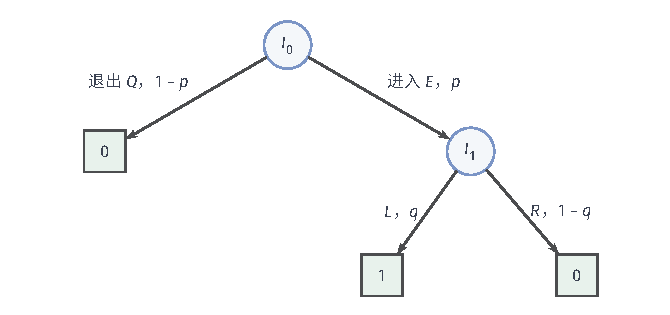
\includegraphics[width=\linewidth]{figures/01-mathematical-preliminaries/05-dynamical-systems-control-decision-and-games/tikz/game-two-stage-self-reach/figure.pdf}
  \caption{同一参与者$i$的两层决策。圆节点是其信息集，方节点中的数值是终局收益。
  第一步以概率$p$进入，第二步在已进入的条件下以概率$q$选$L$；
  因此到达收益为$1$的终局需经过两个本人行动，概率为$pq$。
  本图没有对手或机会节点，是用于区分自身到达概率与局部行动概率的教学构造。}
  \label{fig:game-two-stage-self-reach}
\end{figure}

% Baseline B:972-1018; learning indices normalized
\begin{definition}[反事实价值]
\label{def:game-counterfactual-value}
给定上述联合行为策略及到达权重，参与者\(i\)在信息集\(I\)采取行动\(a\in A(I)\)的
\term{反事实价值}（counterfactual value）定义为
\begin{equation}
  v_i^{\bm{\sigma}}(I,a)
  =
  \sum_{h\in I}
  \pi_{-i}^{\bm{\sigma}}(h)
  \sum_{z\succeq ha}
  \pi^{\bm{\sigma}}(ha,z)u_i(z).
  \label{eq:game-counterfactual-action-value}
\end{equation}
信息集当前策略的反事实价值为
\begin{equation}
  v_i^{\bm{\sigma}}(I)
  =
  \sum_{a\in A(I)}
  \sigma_i(a\mid I)
  v_i^{\bm{\sigma}}(I,a).
  \label{eq:game-counterfactual-value}
\end{equation}

\end{definition}
式~\eqref{eq:game-counterfactual-action-value}保留对手和机会到达\(I\)的权重，
却去掉参与者\(i\)自己在到达\(I\)以前的概率。它在问：假设参与者\(i\)把自己送到
这个信息集，其他方和机会以当前方式到达各节点时，当前行动价值如何。去掉自身到达权重
使一个很少被当前自身策略访问的信息集仍能积累学习信号。

在例~\ref{ex:game-two-stage-self-reach}中，去掉自身前缀概率$p$以后，
$v_i(I_1,L)=1$、$v_i(I_1,R)=0$，当前局部价值为$v_i(I_1)=q$。
选$L$的局部改进量为$1-q$，因而在$p=0$时仍保留信号。
它没有声称当前整局收益已经增加了$1-q$；比较完整替代计划时，
还要补回该计划自己到达$I_1$的概率。

在均衡牌面策略下，参与者2的信息集包含高牌质询与低牌质询两个节点。对参与者2而言，
相应反事实到达权重为
\[
  \frac12 b_H^\star=\frac12,
  \qquad
  \frac12 b_L^\star=\frac16.
\]
若把它们归一化，得到到达信息集后的信念
\[
  \mathbb{P}(H\mid B)=\frac34,\qquad
  \mathbb{P}(L\mid B)=\frac14.
\]
在这组权重下，参与者2选择应对的反事实价值为
$\frac12(-2)+\frac16(2)=-\frac23$，退让的反事实价值为
$(\frac12+\frac16)(-1)=-\frac23$。除以总权重$2/3$后，两项条件期望收益都为$-1$。
局部是否偏好一个行动由同一比例缩放保持，但跨信息集求和必须保留原权重。
后验概率用于该信息集内的条件决策，反事实价值则保留未归一化权重，以便把不同信息集的
局部偏离加回整局收益。两者只差一个到达概率因子，却服务于不同推导。

此处“反事实”不同于第~\ref{chap:causal-inference}章的因果反事实：
前者在既定博弈中去掉本人到达权重，后者固定同一单位的外生背景并替换结构方程。
前者不提供因果识别结论。尤其不能先在每个信息集随意归一化，再把不同位置的条件收益
直接相加充当整局差距。

% Baseline B:1189-1264; learning indices normalized
前两小节采用损失约定，遗憾写成实际损失减替代损失。扩展式博弈沿用收益函数，下面改用
收益约定，把遗憾写成替代收益减当前收益；令损失等于收益的相反数，就能在两种约定之间
转换，正遗憾始终表示偏离更有利。

在第\(k\)轮扩展式博弈中，联合策略记为\(\bm{\sigma}^{(k)}\)。参与者\(i\)在信息集
\(I\)把当前随机行动改成固定行动\(a\)的即时反事实遗憾为
\begin{equation}
  r_i^{(k)}(I,a)
  =
  v_i^{\bm{\sigma}^{(k)}}(I,a)
  -
  v_i^{\bm{\sigma}^{(k)}}(I).
  \label{eq:game-immediate-counterfactual-regret}
\end{equation}
累计量及其正部最大值记为
\[
  R_i^{(K)}(I,a)
  =
  \sum_{k=1}^{K}r_i^{(k)}(I,a),
  \qquad
  R_{i,+}^{(K)}(I)
  =
  \max\left\{0,\max_{a\in A(I)}R_i^{(K)}(I,a)\right\}.
\]

\term{反事实遗憾最小化}（counterfactual regret minimization, CFR）在每个信息集
运行一个局部无遗憾算法\scite{math-zinkevich2007cfr}一次完整树更新包含四步：
固定本轮联合行为策略并遍历历史树，计算各信息集的反事实行动价值；用
式~\eqref{eq:game-immediate-counterfactual-regret}累计每个行动的遗憾；用局部
遗憾匹配生成下一轮策略；同时按本人的到达概率累计平均策略所需的实现权重。这里的
“最小化”是让平均遗憾趋近于零，不是逐轮直接最小化某个静态目标。

典型的\term{遗憾匹配}（regret matching）按正累计遗憾选择下一轮行动：
\begin{equation}
  \sigma_i^{(k+1)}(a\mid I)
  =
  \begin{cases}
    \displaystyle
    \frac{[R_i^{(k)}(I,a)]_+}
         {\sum_b[R_i^{(k)}(I,b)]_+},
      &\sum_b[R_i^{(k)}(I,b)]_+>0,\\[8pt]
    \displaystyle\frac{1}{|A(I)|},
      &\text{否则}.
  \end{cases}
  \label{eq:game-regret-matching}
\end{equation}
所有\(R_i^{(0)}(I,a)\)初始化为零，首轮因此使用均匀分布。

若存在\(\Delta_I\geq0\)，使对每轮\(k=1,\ldots,K\)及任意
\(a,b\in A(I)\)都有
\[
  \left|
    v_i^{\bm{\sigma}^{(k)}}(I,a)
    -
    v_i^{\bm{\sigma}^{(k)}}(I,b)
  \right|
  \leq\Delta_I,
\]
则遗憾匹配满足
\begin{equation}
  R_{i,+}^{(K)}(I)
  \leq
  \Delta_I\sqrt{|A(I)|K}.
  \label{eq:game-local-regret-matching-bound}
\end{equation}
证明可用势函数
\(\Phi^{(k)}=\sum_a[R_i^{(k)}(I,a)]_+^2\)，其中\(\Phi^{(0)}=0\)。
对任意实数\(x,y\)，有
\([x+y]_+^2\leq[x]_+^2+2[x]_+y+y^2\)；
将它用于累计遗憾递推，每轮势函数增量中的交叉项为
\[
  2\sum_a[R_i^{(k-1)}(I,a)]_+r_i^{(k)}(I,a).
\]
当正遗憾和非零时，式~\eqref{eq:game-regret-matching}使它正比于
\(\sum_a\sigma_i^{(k)}(a\mid I)r_i^{(k)}(I,a)=0\)；正遗憾和为零时，
交叉项也不为正。平方增量至多
\(\sum_a(r_i^{(k)}(I,a))^2\leq |A(I)|\Delta_I^2\)。
归纳得到
\(\Phi^{(K)}\leq K|A(I)|\Delta_I^2\)，而每个正累计遗憾的平方不超过
\(\Phi^{(K)}\)，于是得到式~\eqref{eq:game-local-regret-matching-bound}。

% Baseline B:1268-1297; learning indices normalized
用三张牌博弈核对一次参与者2的CFR更新。假设当前策略取
\[
  b_H=b_L=\frac12,\qquad
  \sigma_2(C\mid I_2)=\sigma_2(F\mid I_2)=\frac12.
\]
参与者2到达高牌质询节点和低牌质询节点的反事实权重都为
\[
  \frac12\cdot\frac12=\frac14.
\]
第一个因子来自机会发牌，第二个因子来自参与者1质询。应对
\(C\)时，参与者2在高牌和低牌节点的收益分别为\(-2\)与\(2\)，所以
\[
  v_2(I_2,C)
  =
  \frac14(-2)+\frac14(2)=0.
\]
退让\(F\)时，参与者1在两个节点都得到\(1\)，参与者2因而都得到\(-1\)，所以
\[
  v_2(I_2,F)
  =
  \frac14(-1)+\frac14(-1)=-\frac12.
\]
当前均匀策略的反事实价值为\(-1/4\)，本轮即时遗憾因此为
\[
  r_2(I_2,C)=\frac14,\qquad
  r_2(I_2,F)=-\frac14.
\]
若此前累计遗憾为零，遗憾匹配在下一轮把全部概率放到\(C\)。这个结果只描述一次局部
更新；参与者2更常应对以后，低牌质询会变得不利，参与者1的后续更新又会改变两个节点的
权重。因而不能把首轮纯响应当成收敛策略，也不能从这一个数值步骤推出均衡保证。

\subsubsection{完全回忆下的局部遗憾汇总}
\label{sec:game-perfect-recall-regret}

局部无遗憾尚未回答完整策略能改善多少。证明须把对手与机会的到达权重留在局部量中，
再用同一个替代策略的自身到达概率汇总；完全回忆保证汇总时每条本人决策前缀不含歧义。

% Baseline B:1301-1478; learning indices normalized
整局外部遗憾允许参与者把当前行为策略替换成任意固定行为策略：
\begin{equation}
  R_i^{(K)}
  =
  \max_{\widetilde{\sigma}_i}
  \sum_{k=1}^{K}
  \left[
    u_i(\widetilde{\sigma}_i,\bm{\sigma}_{-i}^{(k)})
    -
    u_i(\bm{\sigma}^{(k)})
  \right].
  \label{eq:game-extensive-external-regret}
\end{equation}
局部反事实遗憾之所以有用，在于它们能够上界这个看似覆盖整棵树的比较。

例~\ref{ex:game-two-stage-self-reach}可以先展示一次拆分。
当前策略为$(p,q)$，完整替代策略为$(\widetilde p,\widetilde q)$时，
\begin{equation}
 \widetilde p\,\widetilde q-pq
 =(\widetilde p-p)q+\widetilde p(\widetilde q-q).
 \label{eq:game-two-stage-deviation}
\end{equation}
第一项只改$I_0$的进入概率，保留当前第二步$q$；
第二项再改$I_1$的行动，乘上的却是替代计划的进入概率$\widetilde p$。
第二步的局部改进先去掉当前自身权重$p$，在完整计划比较中再补回$\widetilde p$，
就能同时处理上游和下游都改变的情况。例如$p=q=0$、$\widetilde p=\widetilde q=1$时，
第一项为零，第二项为$1$，恰好恢复整局收益的增加。
下面把这项拆分沿所有本人信息集重复。

\begin{theorem}[CFR的反事实遗憾分解]
\label{thm:game-cfr-decomposition}
在有限完全回忆扩展式博弈中，
\begin{equation}
  R_i^{(K)}
  \leq
  \sum_{I\in\mathcal{I}_i}
  R_{i,+}^{(K)}(I).
  \label{eq:game-cfr-global-bound}
\end{equation}
\end{theorem}

\begin{proof}
固定替代行为策略\(\widetilde{\sigma}_i\)。证明先在一轮中把整局偏离逐层拆开，再对
轮次求和。为看清拆分发生在哪里，对\(h\in I\)定义当前策略在行动\(a\)后的条件续局
收益
\[
  q_i^{(k)}(h,a)
  =
  \sum_{z\succeq ha}
  \pi^{\bm{\sigma}^{(k)}}(ha,z)u_i(z),
\]
并以\(\widetilde q_i^{(k)}(h,a)\)表示对手和机会仍采用
\(\bm{\sigma}_{-i}^{(k)}\)，而参与者\(i\)从\(ha\)以后采用
\(\widetilde{\sigma}_i\)时的同一数值，即
\[
  \widetilde q_i^{(k)}(h,a)
  =
  \sum_{z\succeq ha}
  \pi^{(\widetilde{\sigma}_i,\bm{\sigma}_{-i}^{(k)})}(ha,z)
  u_i(z).
\]
当前策略从\(h\)出发的续局收益为
\(q_i^{(k)}(h)=\sum_b\sigma_i^{(k)}(b\mid I)q_i^{(k)}(h,b)\)。
在替代收益中加上再减去“只在当前行动改用替代分布、以后仍用当前策略”的收益，逐历史
得到恒等式
\begin{align}
  &\sum_{a\in A(I)}
  \widetilde{\sigma}_i(a\mid I)
  \widetilde q_i^{(k)}(h,a)
  -
  q_i^{(k)}(h)
  \notag\\
  &\quad=
  \sum_{a\in A(I)}
  \widetilde{\sigma}_i(a\mid I)
  \bigl(q_i^{(k)}(h,a)-q_i^{(k)}(h)\bigr)
  \notag\\
  &\qquad\quad+
  \sum_{a\in A(I)}
  \widetilde{\sigma}_i(a\mid I)
  \bigl(
    \widetilde q_i^{(k)}(h,a)-q_i^{(k)}(h,a)
  \bigr).
  \label{eq:game-history-deviation-identity}
\end{align}
第一项只改变当前信息集的行动，第二项只记录当前行动之后继续偏离的收益。

下面把逐历史恒等式汇总到信息集。记
\(\mathcal{C}_i(I,a)\)为采取\(a\)以后、在参与者\(i\)再次行动时首次遇到的本人
信息集集合；若在此之前终止，就没有后继信息集。令
\(\widetilde v_i^{(k)}(I)\)为到达\(I\)的对手与机会权重仍取
\(\pi_{-i}^{\bm{\sigma}^{(k)}}(h)\)，但从\(I\)起参与者\(i\)都采用
\(\widetilde{\sigma}_i\)的反事实价值，并记
\[
  D_i^{(k)}(I)
  =
  \widetilde v_i^{(k)}(I)
  -
  v_i^{\bm{\sigma}^{(k)}}(I),
  \qquad
  L_i^{(k)}(I)
  =
  \sum_a
  \widetilde{\sigma}_i(a\mid I)r_i^{(k)}(I,a).
\]
将式~\eqref{eq:game-history-deviation-identity}乘以
\(\pi_{-i}^{\bm{\sigma}^{(k)}}(h)\)并对\(h\in I\)求和，得到信息集偏离收益恒等式
\begin{equation}
  D_i^{(k)}(I)
  =
  L_i^{(k)}(I)
  +
  \sum_{a\in A(I)}
  \widetilde{\sigma}_i(a\mid I)
  \sum_{I'\in\mathcal{C}_i(I,a)}
  D_i^{(k)}(I').
  \label{eq:game-information-set-deviation-identity}
\end{equation}
这里没有漏掉从\(I\)到\(I'\)之间的概率：这段路径上参与者\(i\)不再行动，对手和
机会的路径概率与\(I\)处已有的权重相乘，正好成为\(I'\)中各历史的
\(\pi_{-i}^{\bm{\sigma}^{(k)}}\)。在遇到下一个本人信息集以前终止的路径上，两种
策略的后续行为相同，故其第二项为零。

完全回忆使本人信息集及边\((I,a)\to I'\)组成一个森林。确切地说，同一信息集
\(I'\)中的所有历史具有相同的本人既往信息集与行动序列，所以每个非根信息集都有唯一的
前驱边；对手或机会的多条历史可以汇入同一个\(I'\)，但这些历史只在
\(\pi_{-i}^{\bm{\sigma}^{(k)}}\)的求和中合并，不会把\(I'\)复制成多个后继。
记\(\widetilde{\pi}_i(I)\)为替代策略沿该唯一本人前缀的行动概率乘积；根信息集的
乘积约定为\(1\)。这正是反事实价值中故意省去的自身到达概率。

现在按一个信息集之后还可能遇到的本人信息集层数归纳。最深信息集没有后继，
式~\eqref{eq:game-information-set-deviation-identity}给出
\(D_i^{(k)}(I)=L_i^{(k)}(I)\)。假设所有深度更小的后继子树都已展开，把它们代回
同一恒等式；由于每个后继只有一个前驱，子树中的每个信息集恰好出现一次，其系数等于
沿唯一前缀的\(\widetilde{\sigma}_i\)行动概率乘积。对森林的所有根求和后便得到
\begin{equation}
  u_i(\widetilde{\sigma}_i,\bm{\sigma}_{-i}^{(k)})
  -
  u_i(\bm{\sigma}^{(k)})
  =
  \sum_{I\in\mathcal{I}_i}
  \widetilde{\pi}_i(I)
  \sum_{a\in A(I)}
  \widetilde{\sigma}_i(a\mid I)r_i^{(k)}(I,a).
  \label{eq:game-global-deviation-identity}
\end{equation}
参与者\(i\)从未行动就终止的历史在两种策略下收益相同，因而不出现在右侧。
式~\eqref{eq:game-global-deviation-identity}明确分开了两类权重：对手与机会的权重
已经包含在\(r_i^{(k)}(I,a)\)中，自身在替代策略下到达\(I\)的权重则是外部系数
\(\widetilde{\pi}_i(I)\)。

替代策略固定后，\(\widetilde{\pi}_i(I)\)和
\(\widetilde{\sigma}_i(a\mid I)\)都不随\(k\)变化。对
式~\eqref{eq:game-global-deviation-identity}求和，并使用
\(0\leq\widetilde{\pi}_i(I)\leq1\)，可得
\begin{align*}
  &\sum_{k=1}^{K}
  \left[
    u_i(\widetilde{\sigma}_i,\bm{\sigma}_{-i}^{(k)})
    -
    u_i(\bm{\sigma}^{(k)})
  \right]\\
  &\quad=
  \sum_I
  \widetilde{\pi}_i(I)
  \sum_a
  \widetilde{\sigma}_i(a\mid I)R_i^{(K)}(I,a)\\
  &\quad\leq
  \sum_I
  \widetilde{\pi}_i(I)
  \max_a R_i^{(K)}(I,a)
  \leq
  \sum_I R_{i,+}^{(K)}(I).
\end{align*}
最后一个不等式也覆盖\(\max_aR_i^{(K)}(I,a)<0\)的情形，因为此时相应正部为零。
右侧与替代策略无关，再对\(\widetilde{\sigma}_i\)取最大，就得到
式~\eqref{eq:game-cfr-global-bound}。
\end{proof}

若缺少完全回忆，同一当前信息集可能汇合不同的本人行动历史。此时局部策略无法知道应该
补回哪条自身到达路径，上述递归可能重复计算或遗漏偏离收益，局部低遗憾便不再自动控制
整局外部遗憾。

结合式~\eqref{eq:game-local-regret-matching-bound}，CFR得到
\begin{equation}
  R_i^{(K)}
  \leq
  \sum_{I\in\mathcal{I}_i}
  \Delta_I\sqrt{|A(I)|K}.
  \label{eq:game-cfr-rate}
\end{equation}
当信息集和行动数固定时，平均正外部遗憾
\([R_i^{(K)}]_+/K=O(K^{-1/2})\)，因而趋于零。

有限树与有界终局收益保证可以为各信息集选择有限的\(\Delta_I\)。
这个界针对遍历完整树、准确计算反事实价值的版本，不依赖末次策略是否单调改善。
若信息集本身改变、遗忘破坏完全回忆，或采样值存在未控制的偏差，
须重新检查分解与局部算法，不能只引用CFR名称。

\subsection{累计保证与平均策略表现}
\label{sec:game-regret-average-guarantees}

累计界要转成均衡误差，还需选对平均方式。一般和博弈保留共同轮次形成的联合分布；
两人零和博弈借助收益的分别线性，把双方的独立平均策略与鞍点差距连接起来。
历史树中还须先平均实现计划，才能恢复合法的行为策略。

\subsubsection{一般和条件下的经验分布保证}
\label{sec:game-empirical-equilibrium}

令第\(k\)轮实际联合行动为\(\bm a^{(k)}\)，经验联合分布为
\[
  \widehat\mu^{(K)}(\bm a)
  =\frac1K\sum_{k=1}^K\mathbb I\{\bm a^{(k)}=\bm a\}.
\]
若第\(i\)方的外部收益遗憾不超过\(\varepsilon_iK\)，则对任意固定行动\(a_i'\)，
直接把累计不等式除以\(K\)便得
\[
  \mathbb E_{\bm A\sim\widehat\mu^{(K)}}[u_i(\bm A)]
  \geq
  \mathbb E_{\bm A\sim\widehat\mu^{(K)}}
     [u_i(a_i',\bm A_{-i})]-\varepsilon_i.
\]
这正是第~\ref{sec:game-correlated-deviations}节的CCE不等式加上误差。
若所有参与者的平均正外部遗憾趋零，有限联合单纯形的紧性保证经验分布的每个极限点
都满足CCE条件，也保证其到CCE集合的距离趋零；未必存在唯一的极限分布。

若每个有向替换\(a_i\to b_i\)的平均内部遗憾至多\(\varepsilon_i\)，那么对任意
映射\(\phi_i:A_i\to A_i\)，有
\[
  \begin{aligned}
    &\mathbb E_{\widehat\mu^{(K)}}[
       u_i(\phi_i(A_i),\bm A_{-i})-u_i(\bm A)]\\
    &\qquad=\frac1K\sum_{a_i\in A_i}R_{a_i\to\phi_i(a_i)}^{(K)}
      \leq |A_i|\varepsilon_i.
  \end{aligned}
\]
这里的\(R\)已改写为收益约定。有限个有向替换控制了所有按建议改动的映射，所以
无内部遗憾给出经验联合分布的CE极限点。若算法直接控制所有映射的交换遗憾，
松弛就是\(\varepsilon_i\)，不必再乘\(|A_i|\)。
这个比较不会把普通外部遗憾算法自动升级为内部遗憾算法。

保留联合相关性确实必要。例如双方行动均为\(A,B\)，以第1方的行动为行、
第2方的行动为列，各格列出双方收益：
\[
  \begin{array}{c|cc}
     &A&B\\ \hline
    A&(2,2)&(0,0)\\
    B&(0,0)&(1,1)
  \end{array}
\]
若实际序列一半轮次为\((A,A)\)、一半为\((B,B)\)，每人平均得\(3/2\)，
改用固定\(A\)只能得\(1\)，改用固定\(B\)只能得\(1/2\)；按建议单独改动也无利。
经验分布是CE。两方边缘平均却都是\((1/2,1/2)\)，将它们独立相乘后，
一方对该边缘选\(A\)得\(1\)、选\(B\)得\(1/2\)，混合只得\(3/4\)，所以平均边缘
的乘积不是Nash均衡。

这些是对已记录联合序列的代数结论。若算法控制的是期望损失遗憾，而这里使用抽样行动，
还须估计两者之间的随机误差；每轮独立抽样也不消除跨轮共同变化产生的相关性。

\subsubsection{零和条件下的平均策略保证}
\label{sec:game-zero-sum-average}

矩阵博弈中，\(\bar{\bm x}^{(K)}=K^{-1}\sum_k\bm x^{(k)}\)与
\(\bar{\bm y}^{(K)}=K^{-1}\sum_k\bm y^{(k)}\)仍在各自单纯形内。
固定一方策略时，双线性收益可把另一方的平均移进或移出求和。
历史树中的行为概率却在同一条路径上相乘，逐信息集算术平均一般没有这项性质。

仍用例~\ref{ex:game-two-stage-self-reach}的小树，考虑表~\ref{tab:game-two-stage-average}中的两轮策略。
先等概率抽取一轮，再执行该轮的完整策略，终局$L$的概率为$(1+0)/2=1/2$。
若分别平均两个节点的行动概率，就会得到$\bar p=\bar q=1/2$，
从而把终局$L$的概率改成$\bar p\bar q=1/4$。
错误来自第二轮的$q^{(2)}=0$：这一轮始终退出，第二步怎样选择本来都没有作用，
普通平均却把这个未执行的安排与第一轮同等计入。

\begin{table}[htbp]
  \centering
  \setlength{\tabcolsep}{4pt}
  \begin{tabular}{cccc}
    \toprule
    轮次$k$ & $p^{(k)}$ & $q^{(k)}$ & 终局$L$概率\\
    \midrule
    $1$ & $1$ & $1$ & $1$\\
    $2$ & $0$ & $0$ & $0$\\
    \bottomrule
  \end{tabular}
  \caption{两层小树中的两轮完整策略。$p^{(k)}$表示进入概率，$q^{(k)}$表示进入后选$L$的概率，
  最后一列为$p^{(k)}q^{(k)}$。第二轮不进入，故该轮第二步的安排不影响终局分布。
  这些数值只用于比较策略平均方式，不表示CFR必然产生这样的两轮轨迹。}
  \label{tab:game-two-stage-average}
\end{table}

按本人到达权重平均第二步，则
\[
 \bar q=
 \frac{p^{(1)}q^{(1)}+p^{(2)}q^{(2)}}{p^{(1)}+p^{(2)}}=1,
 \qquad \bar p=\frac12,
\]
使$\bar p\bar q=1/2$，恢复完整策略混合的终局概率。
若两轮都不进入，分母为零，此时任意$\bar q$都与$\bar p=0$组合成相同终局分布。
这个计算依赖$I_1$有唯一本人前缀$I_0\xrightarrow{E}I_1$；
完全回忆把这一性质推广到一般信息集，才能逐层恢复平均后的实现权重。

% Baseline B:1482-1608; learning indices normalized
行为策略不能在每个信息集直接做普通算术平均。某轮中一个信息集若几乎不会被参与者自己
到达，该处局部概率不应与频繁到达轮次具有同样权重。完全回忆保证同一信息集
\(I\)中的历史具有同一条本人行动前缀，因而
\(\pi_i^{\bm{\sigma}^{(k)}}(I)\)定义为这条前缀上的本人行动概率乘积，与选取
哪个\(h\in I\)无关。记第\(k\)轮在本人序列\((I,a)\)上的实现权重为
\[
  x_i^{(k)}(I,a)
  =
  \pi_i^{\bm{\sigma}^{(k)}}(I)
  \sigma_i^{(k)}(a\mid I),
\]
并令
\(\overline{x}_i^{(K)}(I,a)=K^{-1}\sum_k x_i^{(k)}(I,a)\)以及
\(\overline{x}_i^{(K)}(I)=K^{-1}\sum_k
\pi_i^{\bm{\sigma}^{(k)}}(I)\)。CFR使用
\begin{equation}
  \overline{\sigma}_i^{(K)}(a\mid I)
  =
  \frac{
    \sum_{k=1}^{K}
    \pi_i^{\bm{\sigma}^{(k)}}(I)
    \sigma_i^{(k)}(a\mid I)
  }{
    \sum_{k=1}^{K}
    \pi_i^{\bm{\sigma}^{(k)}}(I)
  },
  \label{eq:game-cfr-average-strategy}
\end{equation}
其中分母为零时可以任意指定。式~\eqref{eq:game-cfr-average-strategy}等价于
\[
  \overline{\sigma}_i^{(K)}(a\mid I)
  =
  \frac{\overline{x}_i^{(K)}(I,a)}{\overline{x}_i^{(K)}(I)}.
\]

这个权重不是经验修正，而是实现计划平均所要求的条件概率。根本人序列的实现权重为
\(1\)。若\(I\)的唯一本人前驱序列终止于\((J,b)\)，则每一轮都有
\(\pi_i^{\bm{\sigma}^{(k)}}(I)=x_i^{(k)}(J,b)\)，对轮次平均后仍有
\(\overline{x}_i^{(K)}(I)=\overline{x}_i^{(K)}(J,b)\)。从根序列归纳，并在每个信息集应用
上面的条件概率公式，得到
\begin{equation}
  \pi_i^{\overline{\sigma}_i^{(K)}}(I)
  \overline{\sigma}_i^{(K)}(a\mid I)
  =
  \overline{x}_i^{(K)}(I,a)
  =
  \frac{1}{K}\sum_{k=1}^{K}x_i^{(k)}(I,a).
  \label{eq:game-average-realization-plan}
\end{equation}
因此，加权平均行为策略实现的正是各轮本人实现计划的算术平均。分母为零意味着所有轮次
到达该本人序列的概率都为零，此处怎样指定局部策略都不改变平均实现计划。

在两人零和博弈中，若双方累计外部遗憾分别不超过
\(\varepsilon_1K\)与\(\varepsilon_2K\)，则平均策略满足
\begin{equation}
  \max_{\sigma_1}
  u_1(\sigma_1,\overline{\sigma}_2^{(K)})
  -
  \min_{\sigma_2}
  u_1(\overline{\sigma}_1^{(K)},\sigma_2)
  \leq
  \varepsilon_1+\varepsilon_2.
  \label{eq:game-average-exploitability}
\end{equation}
下面补出这个界。记第\(k\)轮第1位参与者的收益为
\(u_1(\sigma_1^{(k)},\sigma_2^{(k)})\)，并令
\[
  \widehat u^{(K)}
  =
  \frac{1}{K}
  \sum_{k=1}^{K}
  u_1(\sigma_1^{(k)},\sigma_2^{(k)}).
\]
终止历史\(z\)的概率可以写成机会概率与双方实现权重之积，所以期望收益对双方实现计划
分别线性。结合式~\eqref{eq:game-average-realization-plan}，对任意固定策略
\(\sigma_1,\sigma_2\)有
\begin{align}
  \frac{1}{K}\sum_{k=1}^{K}
  u_1(\sigma_1,\sigma_2^{(k)})
  &=
  u_1(\sigma_1,\overline{\sigma}_2^{(K)}),
  \notag\\
  \frac{1}{K}\sum_{k=1}^{K}
  u_1(\sigma_1^{(k)},\sigma_2)
  &=
  u_1(\overline{\sigma}_1^{(K)},\sigma_2).
  \label{eq:game-average-payoff-linearity}
\end{align}

第1位参与者的外部遗憾界除以\(K\)，再用第一条等式，得到
\begin{equation}
  \max_{\sigma_1}
  u_1(\sigma_1,\overline{\sigma}_2^{(K)})
  -
  \widehat u^{(K)}
  \leq
  \varepsilon_1.
  \label{eq:game-row-average-regret}
\end{equation}
第2位参与者的收益为\(u_2=-u_1\)。把其外部遗憾界同样除以\(K\)，并用
式~\eqref{eq:game-average-payoff-linearity}的第二条等式，得到
\begin{equation}
  \widehat u^{(K)}
  -
  \min_{\sigma_2}
  u_1(\overline{\sigma}_1^{(K)},\sigma_2)
  \leq
  \varepsilon_2.
  \label{eq:game-column-average-regret}
\end{equation}
将式~\eqref{eq:game-row-average-regret}与
\eqref{eq:game-column-average-regret}相加，经验对局收益
\(\widehat u^{(K)}\)消去，正好得到
式~\eqref{eq:game-average-exploitability}。若博弈值为\(v^\star\)，其左侧还可写成
\[
  \left[
    \max_{\sigma_1}u_1(\sigma_1,\overline{\sigma}_2^{(K)})-v^\star
  \right]
  +
  \left[
    v^\star-\min_{\sigma_2}u_1(\overline{\sigma}_1^{(K)},\sigma_2)
  \right].
\]
两项分别衡量第2位和第1位参与者的平均策略可被最佳响应利用多少，且都非负；因此该和是
双方平均策略的零和鞍点间隙。本章把这个和称为\term{联合可利用度}
（joint exploitability）；若采用两项平均的口径，数值还需除以\(2\)。间隙为零时，
两者构成极小极大策略对。

一个两步单方例能看清权重的作用：首步以概率\(p\)继续，继续后以概率\(q\)选\(a\)。
两轮采用\((p^{(1)},q^{(1)})=(1,1)\)、\((p^{(2)},q^{(2)})=(0,0)\)。
两轮平均到达终局\(a\)的概率为\(1/2\)。若分别算术平均，得到\(p=q=1/2\)，
终局概率变成\(1/4\)，并未实现原平均。按自身到达概率加权则得到
\(\bar p=1/2,\bar q=(1\cdot1+0\cdot0)/(1+0)=1\)，恢复正确的\(1/2\)。
三张牌中每人只行动一次，各自信息集没有本人先前行动，权重恰好都为\(1\)；
因此这个特例可以直接平均\(b_H,b_L,c\)，不能据此推广到多步决策。

式~\eqref{eq:game-average-exploitability}保证的是两人零和博弈的平均策略，而非末项。
有限完全回忆时，合法平均和极小极大结构共同支持这项结论；一般和的联合经验分布
结论已在上一小节单独建立。

% Baseline B:1637-1664; learning indices normalized
末次策略还可能持续循环。采样CFR若只访问部分历史，还要用第
\ref{chap:stochastic-processes-and-approximation}章的无偏估计、方差和集中工具控制
采样误差，不能把完整树上的确定性分解直接当作有限样本保证。

回到三张牌例子，参与者2的信息集使用高牌质询权重\(1/2\)和低牌质询权重\(1/6\)
计算局部应对遗憾。若算法长期发现应对比退让更好，就提高\(C\)的概率；这一变化又会
降低低牌质询的收益，使参与者1减少虚张声势。双方局部更新相互改变下一轮价值，CFR保证
累计偏离受控，却不要求这两个概率逐轮单调走向\(1/3\)。

把平均遗憾转成均衡结论时，还要保留产生平均的联合样本。
表~\ref{tab:game-regret-comparison-conclusions}比较两种偏离：固定行动只提出一个
事前替代选择，内部替换可以对某种已采取行动单独修改，因此后者需要控制更多比较。
这里的保证针对经验联合分布或相应的平均策略，不对最后一轮作同样承诺。

\begin{table*}[htbp]
  \centering
  \begin{tabularx}{\linewidth}{lXXX}
    \toprule
    偏离比较 & 允许怎样改变 & 一般和下的平均结论 & 两人零和的补充\\
    \midrule
    外部遗憾 & 所有轮次统一改用一个固定行动 & 经验联合分布的粗相关偏离收益小 & 双方平均策略的鞍点差距小\\
    内部遗憾 & 将某种已选行动统一换成另一行动 & 经验联合分布的相关偏离收益小 & 仍需按具体信息结构恢复策略\\
    \bottomrule
  \end{tabularx}
  \caption{遗憾的比较类与平均结论。表中要求每位参与者都控制相应的平均遗憾；
  扩展式博弈的平均行为策略还须使用自身到达权重。末次策略收敛不由这些平均结论推出。}
  \label{tab:game-regret-comparison-conclusions}
\end{table*}

\section{本章小结}
\label{sec:game-theory-and-multi-agent-decision-summary}

多方选择使行动的后果取决于联合策略。信息集先限制每人能够实施的完整计划，
到达概率再把这些计划变成各方整局价值。完全回忆保证混合计划与行为策略的实现等价，
也为后面的局部遗憾分解提供唯一本人前缀。三张牌博弈中，是否看得见隐藏牌会改变
合法策略，不只是改变收益估计。

固定其他策略后可求最佳响应，相互响应形成Nash条件。有限混合均衡的存在由
Sperner、Brouwer、闭图近似选择和Kakutani的证明链保证，不意味着唯一、容易计算或
能够被任意学习过程找到。零和极小极大把双方保证写成一对线性规划，三张牌的
\(2/3\)由原对偶可行证书共同确认。共同建议则改变偏离时可用的信息，得到CE与CCE
各自的约束；它们不能与独立混合Nash无条件互换。

给定更新规则以后，才能检验其不动点和稳定性。双加热器的一步响应误差可以收缩，
但这与局内温差在固定反馈下的衰减是两套计算。匹配硬币同时响应会形成四周期，
同时离散梯度在中心附近会放大扰动，连续梯度或复制动态还可能沿闭轨道运行。
ESS另行检验少量新策略的入侵，不能用名称中的“稳定”代替指定更新的分析。

没有末项收敛时，累计比较仍有意义。投影次梯度用固定比较点的距离递推给出
\(O(\sqrt K)\)外部遗憾；CFR保留对手与机会的反事实权重，再沿完全回忆的信息集
森林汇总局部偏离。一般和无外部或内部遗憾控制相应的经验CCE或CE误差，
两人零和的双方遗憾则控制合法平均策略的联合可利用度。平均行为策略须由平均实现
计划恢复，不能逐位置任意平均，也不能把完整树的确定性证明当作采样保证。

合作价值回答另一类问题。Shapley值在联盟价值已定义后按加入顺序平均边际贡献，
并由四项公理唯一刻画；它既不保证成员不退出，也不把预测归因变成因果贡献。
核心检验联盟阻挡，Pareto条件排除共同改善，Nash乘积协商在声明的紧凸可行域、
共同严格增益和分歧点下选择唯一收益向量。公平分配、无获利偏离、动态稳定、
末项收敛和无遗憾各有比较对象与条件，任何一项都不能仅凭另一项的名称推出。
下一章将把这些保证放回后续机器学习任务，比较它们各自回答的问题。

